\documentclass[12pt,a4paper]{report}

\usepackage[utf8]{inputenc}
\usepackage[T1]{fontenc}
\usepackage{listings}
\lstdefinelanguage{Solidity}{
  keywords={pragma,solidity,contract,function,returns,external,internal,public,private,
             view,pure,payable,mapping,address,uint256,uint,bool,bytes32,string,
             event,emit,modifier,require,revert,import,is,memory,storage,indexed,
             bytes,keccak256,struct,enum,constructor,fallback,receive},
  sensitive=true,
  comment=[l]{//},
  morecomment=[s]{/*}{*/},
  morestring=[b]",
}
\lstset{
  basicstyle=\ttfamily\scriptsize,
  keywordstyle=\bfseries,
  commentstyle=\color{black!55}\itshape,
  stringstyle=\itshape,
  breaklines=true,
  frame=tb,
  rulecolor=\color{black!55},
  captionpos=b,
  numbers=left,
  numberstyle=\tiny\color{black!55},
  xleftmargin=2em,
}
\IfFileExists{libertine.sty}{%
  \usepackage[mono=false]{libertine}%
  \IfFileExists{zi4.sty}{\usepackage[varqu]{zi4}}{}%
}{%
  \usepackage{lmodern}%
}
\usepackage[protrusion=true,expansion=false]{microtype}
\usepackage[a4paper,width=155mm,top=25mm,bottom=25mm,headheight=15pt]{geometry}
\usepackage{setspace}
\onehalfspacing
\emergencystretch=3em
\hbadness=2000

\usepackage{amsmath,amssymb}
\usepackage{fontawesome5}
\newcommand{\tmarkDone}{\textbf{\faCheck}}
\newcommand{\tmarkNo}{\textbf{\faTimes}}
\newcommand{\tmarkPartial}{\faHourglassHalf}
\newcommand{\tmarkPlanned}{\textcolor{black!55}{\faCircle}}

\usepackage{graphicx}
\usepackage{svg}
\usepackage{xstring}
% Overleaf / self-contained build: figure assets in overleaf/ (SVG, vector PDF; PNG being phased out).
\newcommand*{\ThesisDiagDir}{overleaf/}
\newcommand*{\ThesisSvgPdfDir}{overleaf/SVG > PDF/}
\graphicspath{{overleaf/}{\ThesisSvgPdfDir}{./}}
\svgpath{{overleaf/}}
\svgsetup{inkscapeversion=1, inkscapearea=\ThesisSvgPdfDir}
\pdfimageresolution=300
\makeatletter
\newcommand*{\@thesis@doinclude}[2]{%
  \if\relax\detokenize{#1}\relax
    \includegraphics{#2}%
  \else
    \includegraphics[#1]{#2}%
  \fi
}
\newcommand*{\@thesis@doinclude@svg}[2]{%
  \StrSubstitute{#2}{.svg}{}[\@thesis@svg@base]%
  \includesvg[#1]{\@thesis@svg@base}%
}
\newcommand*{\@thesismissingimg}[1]{%
  \fbox{\parbox{0.92\linewidth}{\scriptsize\centering\ttfamily Missing file: \detokenize{#1}.\\[2pt]Add it to the \texttt{overleaf/} folder and recompile.}}%
}
\newcommand{\ThesisIncludeGraphics}[2][]{%
  \IfEndWith{#2}{.svg}{%
    \IfFileExists{\ThesisDiagDir#2}{%
      \@thesis@doinclude@svg{#1}{#2}}{%
    \IfFileExists{#2}{%
      \@thesis@doinclude@svg{#1}{#2}}{%
      \@thesismissingimg{#2}%
    }}%
  }{%
    \IfFileExists{\ThesisDiagDir#2}{%
      \@thesis@doinclude{#1}{\ThesisDiagDir#2}}{%
    \IfFileExists{#2}{%
      \@thesis@doinclude{#1}{#2}}{%
      \@thesismissingimg{#2}%
    }}%
  }%
}
\makeatother
\newcommand{\TableScreenshotEnd}[2][]{%
  \refstepcounter{table}%
  \if\relax\detokenize{#1}\relax\else\label{#1}\fi%
  \phantomsection%
  \addcontentsline{lot}{table}{\protect\numberline{\thetable}#2}%
}
\usepackage[table]{xcolor}
\usepackage{tikz}
\usetikzlibrary{arrows.meta,positioning,fit,shapes.geometric,calc}
\usepackage{pgfplots}
\usepgfplotslibrary{statistics}
\pgfplotsset{compat=1.18, minor tick num=0}

\usepackage{booktabs}
\usepackage{array}
\usepackage{colortbl}
\usepackage{multirow}
\usepackage{float}
\usepackage{etoolbox}
\usepackage{caption}
\captionsetup{
    labelfont={bf,small},
    textfont={small},
    skip=6pt,
    format=hang
}
\makeatletter
% Compact, professional List of Figures / List of Tables (no tocloft dependency)
\renewcommand*\l@figure{\@dottedtocline{1}{0em}{3.2em}}
\renewcommand*\l@table{\@dottedtocline{1}{0em}{3.8em}}
\makeatother

\newlength{\ThesisTableImgReserve}
\newlength{\ThesisFigImgReserve}
\setlength{\ThesisTableImgReserve}{\dimexpr2\intextsep+0.75\baselineskip\relax}
\setlength{\ThesisFigImgReserve}{\dimexpr2\intextsep+\abovecaptionskip+\belowcaptionskip+4\baselineskip\relax}
\newcommand{\TableImageMaxFit}[1]{%
  \ThesisIncludeGraphics[
    width=0.7\linewidth,
    height=\dimexpr(\textheight-\ThesisTableImgReserve)*7/10\relax,
    keepaspectratio
  ]{#1}%
}
\newcommand{\FigureImageMaxFit}[1]{%
  \ThesisIncludeGraphics[width=\linewidth,height=\dimexpr\textheight-\ThesisFigImgReserve\relax,keepaspectratio]{#1}%
}
\newcommand{\OnePageDiagram}[2][]{%
  \if\relax\detokenize{#1}\relax
    \ThesisIncludeGraphics[width=\linewidth,height=\dimexpr\textheight-\ThesisFigImgReserve\relax,keepaspectratio]{#2}%
  \else
    \ThesisIncludeGraphics[#1,width=\linewidth,height=\dimexpr\textheight-\ThesisFigImgReserve\relax,keepaspectratio]{#2}%
  \fi
}
\newcommand{\HalfWidthDiagram}[1]{%
  \ThesisIncludeGraphics[width=0.5\linewidth,keepaspectratio]{#1}%
}
\newcommand{\WideDiagram}[2][]{%
  \if\relax\detokenize{#1}\relax
    \ThesisIncludeGraphics[width=\linewidth,height=0.78\textheight,keepaspectratio]{#2}%
  \else
    \ThesisIncludeGraphics[#1,width=\linewidth,height=0.78\textheight,keepaspectratio]{#2}%
  \fi
}
\newcommand{\TallDiagram}[2][]{%
  \if\relax\detokenize{#1}\relax
    \ThesisIncludeGraphics[width=\linewidth,height=0.96\textheight,keepaspectratio]{#2}%
  \else
    \ThesisIncludeGraphics[#1,width=\linewidth,height=0.96\textheight,keepaspectratio]{#2}%
  \fi
}
% Balanced layout slot (reference: Figure 4.3 ml-explainability) — wide banded diagrams.
\newcommand{\BalancedDiagram}[2][]{%
  \if\relax\detokenize{#1}\relax
    \ThesisIncludeGraphics[width=\linewidth,height=0.72\textheight,keepaspectratio]{#2}%
  \else
    \ThesisIncludeGraphics[#1,width=\linewidth,height=0.72\textheight,keepaspectratio]{#2}%
  \fi
}
% Activity diagrams — full-height slot for 3× label size.
\newcommand{\ActivityDiagram}[2][]{%
  \if\relax\detokenize{#1}\relax
    \ThesisIncludeGraphics[width=\linewidth,height=\textheight,keepaspectratio]{#2}%
  \else
    \ThesisIncludeGraphics[#1,width=\linewidth,height=\textheight,keepaspectratio]{#2}%
  \fi
}
% Half-size slot (50\% of BalancedDiagram width and height).
\newcommand{\CompactDiagram}[2][]{%
  \if\relax\detokenize{#1}\relax
    \ThesisIncludeGraphics[width=0.5\linewidth,height=0.36\textheight,keepaspectratio]{#2}%
  \else
    \ThesisIncludeGraphics[#1,width=0.5\linewidth,height=0.36\textheight,keepaspectratio]{#2}%
  \fi
}

\usepackage[skins]{tcolorbox}

\usepackage{titlesec}
\usepackage{parskip}
\usepackage{fancyhdr}
\usepackage{enumitem}
\PassOptionsToPackage{hyphens,spaces,obeyspaces}{url}
\usepackage{hyperref}
\makeatletter
\g@addto@macro\UrlBreaks{\do\/\do\-\do\.\do\:\do\&\do\=\do\#}
\makeatother

\definecolor{PrimaryBlue}{HTML}{000000}
\definecolor{AccentBlue}{gray}{0.55}
\definecolor{LightBlue}{gray}{0.96}
\definecolor{MidBlue}{gray}{0.90}
\definecolor{DarkText}{HTML}{000000}
\definecolor{GrayText}{gray}{0.45}
\definecolor{RowShade}{gray}{0.965}
\definecolor{RowShadeAlt}{gray}{0.92}
\definecolor{TableHeadBg}{gray}{0.88}
\definecolor{TableRule}{gray}{0.55}
\definecolor{GreenAccent}{HTML}{000000}
\definecolor{AmberAccent}{HTML}{000000}
\definecolor{RedAccent}{HTML}{000000}
\definecolor{VioletAccent}{HTML}{000000}

\hypersetup{
    colorlinks=true,
    linkcolor=black,
    filecolor=black,
    urlcolor=black,
    citecolor=black,
    pdfborder={0 0 0},
}

\titleformat{\chapter}[display]
    {\normalfont\LARGE\bfseries}
    {\chaptertitlename\ \thechapter}{20pt}{\LARGE}
    [\vspace{4pt}{\color{black!40}\titlerule[0.6pt]}]

\titleformat{\section}
    {\large\bfseries}
    {\thesection}{0.8em}{}

\titleformat{\subsection}
    {\normalsize\bfseries}
    {\thesubsection}{0.6em}{}

\titleformat{\subsubsection}
    {\normalsize\bfseries\itshape}
    {\thesubsubsection}{0.6em}{}

\titlespacing*{\chapter}{0pt}{-20pt}{20pt}
\titlespacing*{\section}{0pt}{16pt plus 3pt minus 2pt}{8pt plus 2pt minus 1pt}
\titlespacing*{\subsection}{0pt}{12pt plus 2pt minus 1pt}{6pt plus 1pt minus 1pt}
\titlespacing*{\subsubsection}{0pt}{10pt plus 2pt minus 1pt}{4pt plus 1pt minus 1pt}

\newcommand{\tableheadcolor}{\rowcolor{TableHeadBg}}
\newcommand{\tableheadfont}{\bfseries}
\newcommand{\ThesisTableBodyFont}{\small}

% Consistent greyscale table polish (font size unchanged; spacing only).
\newcommand{\ThesisTablePrep}{%
  \ThesisTableBodyFont
  \renewcommand{\arraystretch}{1.22}%
  \setlength{\tabcolsep}{6pt}%
  \arrayrulecolor{TableRule}%
  \setlength{\aboverulesep}{0.55ex}%
  \setlength{\belowrulesep}{0.55ex}%
}
\AtBeginEnvironment{table}{\ThesisTablePrep}
\AtBeginEnvironment{tabular}{%
  \rowcolors{2}{}{RowShade}%
  \arrayrulecolor{TableRule}%
}

\newenvironment{moderntable}[1][H]{%
    \begin{table}[#1]\centering\ThesisTablePrep
}{%
    \end{table}%
}

\newtcolorbox{layerbox}[1]{
    colback=white,
    colframe=black!55,
    coltitle=black,
    fonttitle=\bfseries\small,
    title=#1,
    boxrule=0.6pt,
    arc=2pt,
    left=6pt,right=6pt,top=4pt,bottom=4pt,
}

\newtcolorbox{highlightbox}[1][]{
    colback=black!4,
    colframe=black!45,
    boxrule=0.5pt,
    arc=2pt,
    left=8pt,right=8pt,top=6pt,bottom=6pt,
    #1
}

\pagestyle{fancy}
\fancyhf{}
\renewcommand{\headrulewidth}{0.4pt}
\fancyhead[L]{\small\color{black!55}Crypto World Bank}
\fancyhead[R]{\small\color{black!55}BRAC University}
\fancyfoot[C]{\small\color{black!55}\thepage}

\newcommand{\manualpie}[6]{%
  \fill[#6] (#1,#2) -- ++({#4}:{#3}) arc ({#4}:{#5}:{#3}) -- cycle;
  \draw[white, line width=0.8pt] (#1,#2) -- ++({#4}:{#3}) arc ({#4}:{#5}:{#3}) -- cycle;
}
\newcommand{\ddcat}[3]{\node[draw=black!55,fill=black!5,rounded corners=2pt,
  minimum width=2.2cm,minimum height=0.65cm,align=center,font=\scriptsize]
  (#1) at (#2) {#3};}
\newcommand{\ddone}[3]{\node[draw=black,fill=black!22,
  minimum width=2.2cm,minimum height=0.65cm,align=center,
  font=\scriptsize\bfseries,rounded corners=2pt] (#1) at #2 {#3};}
\newcommand{\ddtwo}[3]{\node[draw=black!55,fill=white,
  minimum width=2.2cm,minimum height=0.65cm,align=center,
  font=\scriptsize,rounded corners=2pt] (#1) at #2 {#3};}

\begin{document}

%% ============================================================
%% TITLE PAGE
%% ============================================================
\thispagestyle{empty}

\begin{center}

\vspace*{0.3cm}

\ThesisIncludeGraphics[width=3.5cm]{bracu_logo_12-0-2022.svg}

\vspace{0.8cm}

{\LARGE\bfseries\color{PrimaryBlue} Decentralized Crypto World Bank}\\[0.4em]
{\large\color{PrimaryBlue!80} A Blockchain-Based Lending Platform\\[0.15em]with AI-Enhanced Security}

\vspace{0.6cm}

{\normalsize\bfseries Thesis ID: [P26101123]}

\vspace{1.2cm}

{\large by}

\vspace{0.5cm}

{\Large\bfseries\color{PrimaryBlue} Md.\ Bokhtiar Rahman Juboraz}\\[0.2em]
{\color{GrayText}20301138}\\[0.8em]
{\Large\bfseries\color{PrimaryBlue} Md.\ Mahir Ahnaf Ahmed}\\[0.2em]
{\color{GrayText}20301083}

\vspace{1.2cm}

A pre-thesis 1 report submitted to the Department of Computer Science and Engineering\\
in partial fulfillment of the requirements for the degree of\\
\textbf{B.Sc.\ in Computer Science}

\vfill

{\color{PrimaryBlue}\rule{0.4\textwidth}{0.6pt}}\\[0.6em]
Department of Computer Science and Engineering\\
\textbf{BRAC University}\\
February 2026

\vspace{0.5cm}

{\small\color{GrayText}\copyright\ 2026.\ BRAC University --- All rights reserved.}

\end{center}

%% ============================================================
%% DECLARATION
%% ============================================================
\newpage
\thispagestyle{empty}

\chapter*{Declaration}
\phantomsection
\addcontentsline{toc}{chapter}{Declaration}

It is hereby declared that

\begin{enumerate}
\item The report submitted is our own original work while completing degree at BRAC University.

\item The report does not contain material previously published or written by a third party, except where this is appropriately cited through full and accurate referencing.

\item The report does not contain material which has been accepted, or submitted, for any other degree or diploma at a university or other institution.

\item We have acknowledged all main sources of help.
\end{enumerate}

\vspace{2cm}

\textbf{Student's Full Name \& Signature:}

\vspace{2cm}

\begin{tabular}{p{6cm}p{1cm}p{6cm}}
\hrulefill & & \hrulefill \\
\centering Md. Bokhtiar Rahman Juboraz & & \centering Md. Mahir Ahnaf Ahmed \tabularnewline
\centering 20301138 & & \centering 20301083 \tabularnewline
\end{tabular}

%% ============================================================
%% APPROVAL
%% ============================================================
\newpage
\thispagestyle{empty}

\chapter*{Approval}
\phantomsection
\addcontentsline{toc}{chapter}{Approval}

The pre-thesis 1 report of final year project titled ``Decentralized Crypto World Bank: A Blockchain-Based Lending Platform with AI-Enhanced Security'' submitted by

\begin{enumerate}
\item Md. Bokhtiar Rahman Juboraz (20301138)
\item Md. Mahir Ahnaf Ahmed (20301083)
\end{enumerate}

Of Spring, 2026 has been accepted as satisfactory in partial fulfillment of the requirement for the degree of B.Sc. in Computer Science on February 20, 2026.

\vspace{1cm}

\textbf{Examining Committee:}

\vspace{1.5cm}

\begin{flushleft}
Supervisor:\\
(Member)
\end{flushleft}

\begin{flushright}
\vspace{-0.5cm}
\hrulefill\\
Mr. Annajiat Alim Rasel\\
Senior Lecturer\\
Department of Computer Science and Engineering\\
BRAC University
\end{flushright}

\vspace{1.5cm}

\begin{flushleft}
Project Coordinator:\\
(Member)
\end{flushleft}

\begin{flushright}
\vspace{-0.5cm}
\hrulefill\\
Dr. Md. Golam Rabiul Alam\\
Professor\\
Department of Computer Science and Engineering\\
BRAC University
\end{flushright}

\newpage
\thispagestyle{empty}

\null\vfill

\begin{flushleft}
Head of Department:\\
(Chair)
\end{flushleft}

\begin{flushright}
\vspace{-0.5cm}
\hrulefill\\
Dr. Sadia Hamid Kazi\\
Chairperson and Associate Professor\\
Department of Computer Science and Engineering\\
BRAC University
\end{flushright}

\vfill\null

%% ============================================================
%% ETHICS STATEMENT
%% ============================================================
\newpage
\thispagestyle{empty}

\chapter*{Ethics Statement}
\phantomsection
\addcontentsline{toc}{chapter}{Ethics Statement}

This project operates exclusively on public blockchain test networks using test tokens with no real monetary value. No real financial transactions, personal banking data, or user financial records are involved at any stage of development or evaluation. All transaction data used for Artificial Intelligence and Machine Learning (AI/ML) model training and evaluation is either synthetically generated or sourced from publicly available anonymized datasets. The platform prototype does not process Know Your Customer (KYC) or Anti-Money Laundering (AML) data in its current scope, and all wallet addresses used during testing are disposable testnet addresses. We acknowledge the ethical considerations inherent in AI-assisted financial decision-making and have incorporated explainability mechanisms (SHapley Additive exPlanations, or SHAP) to ensure that automated risk assessments remain transparent and auditable by human reviewers. Future phases plan to incorporate a privacy-preserving ZKP-based identity compliance layer in which users prove KYC status without exposing personal data on-chain; the ethical implications of this design will be evaluated in the final thesis.

%% ============================================================
%% ABSTRACT
%% ============================================================
\newpage
\thispagestyle{empty}

\chapter*{Abstract}
\phantomsection
\addcontentsline{toc}{chapter}{Abstract}

Global development finance relies on multilayered institutional structures to distribute capital across borders and communities, yet these systems often struggle with fragmented transparency, procedural friction, and uneven access to credit. Although decentralized finance has demonstrated that programmable infrastructures can automate lending and enhance auditability, existing models largely employ flat architectures that do not reflect institutional hierarchies or structured governance. As a result, there remains limited exploration of how tiered financial systems might be represented within decentralized environments while preserving oversight and adaptability. Here we present \textit{Crypto World Bank}, a formally specified, planning-phase research prototype that specifies a blockchain-based institutional finance platform coordinating capital allocation across a four-tier hierarchical governance structure on EVM-compatible Layer~2 infrastructure. The primary contribution is a smart-contract hierarchy with oracle-mediated risk analytics (Random Forest, Isolation Forest, SHAP via Chainlink Functions); an optional conversational agent (MCP tool server) provides an alternate UI path while core banking remains form- and wallet-driven. The architecture spans six functional domains---deposit mobilization, credit allocation, payment settlement, risk intermediation, liquidity management, and ancillary financial services. Smart contracts, frontend, and oracle integration are specified in this pre-thesis; implementation and testnet deployment are planned across four phases in the final thesis stage. This hybrid design illustrates how institutional finance and decentralized systems may converge, contributing an open-source, hierarchically governed crypto financial services architecture as a foundation for further research.

\vspace{0.5em}
\noindent\textbf{Keywords:} Blockchain, Decentralized Finance, Institutional DeFi, Hierarchical Lending, Smart Contracts, Oracle-Mediated Risk Analytics, Explainable AI, Group Lending, Multi-Entity Co-Lending, Deposit Mobilization, Reserve Management, Financial Sustainability

%% ============================================================
%% DEDICATION
%% ============================================================
\newpage
\thispagestyle{empty}

\chapter*{Dedication}
\phantomsection
\addcontentsline{toc}{chapter}{Dedication}

\vspace{3cm}
\begin{center}
\textit{Dedicated to our families for their unwavering support throughout our academic journey.}
\end{center}

%% ============================================================
%% ACKNOWLEDGMENT
%% ============================================================
\newpage
\thispagestyle{empty}

\chapter*{Acknowledgment}
\phantomsection
\addcontentsline{toc}{chapter}{Acknowledgment}

We would like to express our sincere gratitude to our panel members for their guidance and support throughout this project. We also thank our supervisor, Mr.\ Annajiat Alim Rasel, Senior Lecturer at the Department of Computer Science and Engineering, BRAC University, for his guidance and support. Finally, we thank the Department of Computer Science and Engineering at BRAC University for providing us with the resources and academic environment to pursue this work.

%% ============================================================
%% TABLE OF CONTENTS, LIST OF TABLES, LIST OF FIGURES
%% ============================================================
\newpage
\singlespacing
\setcounter{page}{1}
\pagenumbering{roman}
\tableofcontents
\newpage
\phantomsection
\addcontentsline{toc}{chapter}{List of Tables}
\listoftables
\newpage
\phantomsection
\addcontentsline{toc}{chapter}{List of Figures}
\listoffigures
\newpage
\chapter*{List of Formulas}
\phantomsection
\addcontentsline{toc}{chapter}{List of Formulas}
\begin{description}[leftmargin=0pt]
    \item[Utilization Rate (U):] \(U = \frac{L}{L + B}\) (lending utilization; \(L\) is lent amount, \(B\) is available balance/liquidity)
    \item[Collateral Ratio (CR):] \(CR = \frac{C}{D}\) (collateral-to-debt ratio)
    \item[Loan-to-Value (LTV):] \(LTV = \frac{\text{Loan Amount}}{\text{Collateral Value}}\)
    \item[APR (simple):] \(APR = r_{\text{period}} \times N\) (annualized simple rate over \(N\) periods)
    \item[Compound Interest (Savings):] \(A = P\left(1 + \frac{r}{n}\right)^{nt}\) (deposit growth; \(P\) principal, \(r\) annual rate, \(n\) compounding frequency)
    \item[EMI (Installment Payment):] \(EMI = \frac{P \cdot r \cdot (1+r)^n}{(1+r)^n - 1}\) (installment for principal \(P\), periodic rate \(r\), \(n\) installments)
    \item[Health Factor (HF):] \(HF = \frac{C \times LT}{D}\) (liquidation trigger for \textit{over-collateralized retail loans only}; if \(HF < 1.0\) liquidation is triggered, where \(LT\) is liquidation threshold; see Section~\ref{sec:banking-products} for tier-specific HF variants and the group-loan pool-level formulation)
    \item[Reserve Ratio (RR):] \(RR = \frac{\text{Reserves}}{\text{Total Deposits}}\) (solvency constraint enforced at each tier; governs the maximum downward capital that may be allocated, \textit{not} a money-creation parameter)
    \item[Platform Solvency Ratio (PSR):] \(PSR = \frac{\text{TotalReserveBalance}}{\text{TotalOutstandingLoans}}\) (on-chain analogue of capital adequacy, measuring whether the system's reserve cover exceeds outstanding loan obligations; replaces the Basel~III CAR formula, which is undefined for this platform because USDC assets have no regulatory risk-weight classification under Basel~III and ``Tier~1 Capital'' in the Basel sense cannot be computed from an on-chain USDC balance alone)
    \item[Credit Velocity (CV):] \(CV = \frac{\text{Capital Recycled per Period}}{\text{Total Reserve}}\) (rate at which reserve capital flows through the lending hierarchy and returns as repayment; replaces the inapplicable fractional-reserve money multiplier, which presupposes new money creation and does not apply to fixed-supply USDC)
    \item[FX Conversion:] \(\text{Amount}_B = \text{Amount}_A \times \left(\frac{P_A}{P_B}\right)\) (oracle-priced conversion between assets \(A\) and \(B\))
    \item[Group Loan Individual Share:] \(\text{Share}_i = \frac{\text{LoanTotal}}{N_{\text{members}}}\)
    \item[On-Chain Credit Score (conceptual):] \(CS = \sum_i w_i \cdot \text{feature}_i\) (weighted features learned off-chain and stored as a score on-chain)
    \item[Isolation Forest Anomaly Score:] \(s(x, n) = 2^{-\frac{E(h(x))}{c(n)}}\) (anomaly scoring for instance \(x\); where \(h(x)\) is the path length of instance \(x\) from the root of an isolation tree and \(c(n)\) is the average path length for \(n\) samples)
    \item[Random Forest Fraud Probability:] \(P(\text{fraud}\mid x) = \frac{1}{T}\sum_{t=1}^{T} f_t(x)\) (ensemble average over \(T\) trees; where \(f_t(x)\) is the binary fraud prediction of the \(t\)-th decision tree)
    \item[Platform Net Interest Allocation:] \(\text{NetInterest} = \text{InterestCollected} - \text{DepositorYield} - \text{InsuranceAllocation}\)
    \item[SHAP (Shapley value):] \(\phi_i = \sum_{S \subseteq F \setminus \{i\}} \frac{|S|!(|F|-|S|-1)!}{|F|!}\left[f(S \cup \{i\}) - f(S)\right]\)
\end{description}
\newpage
\chapter*{List of Abbreviations}
\phantomsection
\addcontentsline{toc}{chapter}{List of Abbreviations}
\begin{description}[leftmargin=0pt]
    \item[AA:] Account Abstraction (ERC-4337)
    \item[ALM:] Asset-Liability Management
    \item[AI:] Artificial Intelligence
    \item[AI/ML:] Artificial Intelligence / Machine Learning
    \item[AML:] Anti-Money Laundering
    \item[APR:] Annual Percentage Rate
    \item[API:] Application Programming Interface
    \item[BRAC:] Bangladesh Rural Advancement Committee
    \item[CAR:] Capital Adequacy Ratio (Basel~III; not directly applicable to this platform --- see Platform Solvency Ratio, PSR, in List of Formulas)
    \item[CBDC:] Central Bank Digital Currency
    \item[CCIP:] Cross-Chain Interoperability Protocol (Chainlink)
    \item[CCS:] ACM Computing Classification System
    \item[CR:] Collateral Ratio
    \item[CVL:] Certora Verification Language
    \item[DeFi:] Decentralized Finance
    \item[DID:] Decentralized Identifier (W3C)
    \item[DON:] Decentralised Oracle Network (Chainlink)
    \item[EIP:] Ethereum Improvement Proposal
    \item[EIP-7702:] Ethereum Improvement Proposal 7702 --- Session Key standard enabling scoped, time-bound wallet authorisations for an autonomous agent
    \item[EMI:] Equated Monthly Installment
    \item[ERC:] Ethereum Request for Comments (token / interface standard)
    \item[EVM:] Ethereum Virtual Machine
    \item[FL:] Federated Learning
    \item[FATF:] Financial Action Task Force
    \item[FX:] Foreign Exchange
    \item[GNN:] Graph Neural Network
    \item[HF:] Health Factor
    \item[KYC:] Know Your Customer
    \item[LLM:] Large Language Model
    \item[L2:] Layer 2
    \item[LTV:] Loan-to-Value Ratio
    \item[MFI:] Microfinance Institution
    \item[MiCA:] Markets in Crypto-Assets Regulation (EU)
    \item[ML:] Machine Learning
    \item[MCP:] Model Context Protocol --- tool-calling interface used by the AI agent to interact with CWB banking operations
    \item[NIM:] Net Interest Margin
    \item[PRISMA:] Preferred Reporting Items for Systematic Reviews and Meta-Analyses
    \item[PoS:] Proof of Stake
    \item[PoR:] Proof of Reserve (Chainlink on-chain reserve verification)
    \item[PSR:] Platform Solvency Ratio (on-chain capital adequacy analogue; see List of Formulas)
    \item[QRC:] QR code
    \item[RBAC:] Role-Based Access Control
    \item[RLS:] Row-Level Security (PostgreSQL policy feature enforcing append-only access on audit tables)
    \item[RR:] Reserve Ratio
    \item[SAR:] Suspicious Activity Report
    \item[SBT:] Soulbound Token (non-transferable ERC standard)
    \item[SHAP:] SHapley Additive exPlanations
    \item[SOFR:] Secured Overnight Financing Rate
    \item[SSE:] Server-Sent Events
    \item[SSI:] Self-Sovereign Identity
    \item[SoK:] Systematization of Knowledge
    \item[SWC:] Smart Contract Weakness Classification
    \item[TVL:] Total Value Locked
    \item[U:] Utilization
    \item[UUPS:] Universal Upgradeable Proxy Standard (ERC-1822)
    \item[VC:] Verifiable Credential (W3C)
    \item[XAI:] Explainable Artificial Intelligence
    \item[ZKP:] Zero-Knowledge Proof
    \item[zkAML:] Zero-Knowledge Anti-Money-Laundering proof
    \item[zkEVM:] Zero-Knowledge Ethereum Virtual Machine --- a ZK rollup that inherits Ethereum L1 security via cryptographic validity proofs
    \item[zk-SNARK:] Zero-Knowledge Succinct Non-Interactive Argument of Knowledge
\end{description}
\newpage
\pagenumbering{arabic}
\setcounter{page}{1}


%% CHAPTER 1: INTRODUCTION
\chapter{Introduction}
\label{sec:intro}

The Crypto World Bank is a Final Year research-based project prototype demonstrating the feasibility of a blockchain-based institutional finance platform on programmable blockchain infrastructure. Where existing decentralized finance protocols address isolated financial functions---Aave handles collateralized lending, Uniswap handles exchange, MakerDAO issues stablecoins---the Crypto World Bank formally specifies a hierarchically governed crypto financial services platform spanning the full spectrum of banking functions. These functions include deposit mobilization, credit allocation, installment-based repayment, interbank liquidity management, foreign exchange facilitation, solidarity group lending for retail borrowers, syndicated co-lending and co-funding by groups of institutional entities, reserve enforcement, and risk-based governance---coordinated across four institutional tiers that mirror the structural logic of real-world development finance. The Tier~1 World Bank Reserve and core lending hierarchy are formally specified in Solidity; the multi-entity contract suite (IBLP, SyndicatedLoan, UpwardDepositFacility, TreasurySwap, TranchedPool, NettingEngine) is fully specified in Chapter~3 and scheduled across Phases~II--III.

The system is designed to serve three categories of participants simultaneously. At the global level, it functions as a programmable central reserve institution---managing capital allocation across national jurisdictions with transparent, auditable reserve ratios enforced by smart contract code rather than periodic audit. At the national and regional level, it functions as a commercial and development bank---channeling capital to local lending institutions, managing interbank liquidity, and providing institutional clients with structured credit facilities. At the individual level, it functions as a retail bank---offering savings products, group loans, installment-based personal lending, and digital payment services to Tier~4 clients. Development-finance literature cites large unbanked and MSME financing gaps~[14, 20] as motivation for hierarchical intermediation; this thesis does not claim a specific geographic deployment target. Design artifacts, specifications, and supporting material for this project are available in our \href{https://github.com/Yuvraajrahman/Cryto-World-Bank}{GitHub repository}.

Blockchain functions here as a coordination technology, providing visibility of shared states, audit trails that are difficult to alter, and programmable enforcement of rules among institutions that may have competing interests. Governance design, security controls, and regulatory considerations are incorporated into the platform according to a staged implementation roadmap that includes academic validation and regulatory sandbox pilots. Analogous hybrid institutional structures in blockchain-based finance include the World Bank's FundsChain programme, which tracks fund disbursement across projects on a permissioned ledger, and JPMorgan Kinexys, which settles multi-billion-dollar institutional payments daily on a private EVM-compatible chain---demonstrating that open ledger infrastructure and institutional hierarchy are not mutually exclusive.

Figure~\ref{fig:intro-system-overview} maps the whole-system architecture at a glance: four institutional tiers, the application stack, oracle-mediated analytics, and cross-cutting compliance controls. Detailed layer and component specifications follow in Chapter~\ref{sec:high-level-arch}.

\begin{figure}[H]
\centering
\BalancedDiagram{Ch1_system-overview-four-tier-stack.svg}
\caption[Crypto World Bank system overview]{Whole-system overview: four-tier capital hierarchy (top) and four-layer technology stack (bottom). Reserve ratios, RBAC, oracle-mediated ML, compliance controls, and modular contracts are specified in Chapter~\ref{sec:high-level-arch}.}
\label{fig:intro-system-overview}
\end{figure}

\section{Background}

Understanding why such a system is necessary requires examining the structural failures of the institutions it is designed to complement.

Capital is distributed to local borrowers through layered institutional arrangements in which supranational development institutions such as the World Bank and IMF, national financial intermediaries, and local lenders collaborate to channel development finance to end borrowers. Although this model allows risk sharing and penetrating local markets, it is linked to great operational issues. In cross-border correspondent banking, financial institutions are obligated to have pre-funded nostro and vostro accounts at correspondent banks in every currency corridor, which maroon huge amounts of capital in idle balances unable to be invested or lent out~[24]. Crossborder transactions are regularly settled in two to five business days with an average cost of about \$42 per transaction by using the correspondent banking network~[25]. The remittance market, which is valued at about \$860~billion annually, loses between \$48--56~billion per annum to transfer charges, with the average cost to transfer in the world being 6.49\% as of 2024, more than the United Nations Sustainable Development Goal limit of 3\%~[26].

At the same time, it is estimated that there are 1.4~billion unbanked adults in the world as defined by the World Bank Global Findex~[14], and most of them are found in the developing economies where documentation, geographic location, and minimum balance requirements leave out high populations of people in the formal financial sector. The International Finance Corporation estimates that there is a financing gap in the world of micro, small and medium enterprises at \$4.5~trillion per year~[20], which is unmet credit demand that cannot be effectively met by the existing institutions through the conventional intermediation chains.

The DeFi industry has already shown that lending, collateral management, and interest calculation can be automated on a smart contract platform and that all transactions are transparent, on-chain. The largest DeFi lending protocol, Aave~v3, has amassed \$26.3~billion in total value locked across ten blockchain networks~[27] (accessed March~2026), and the DeFi lending market has more than \$55~billion in TVL~[13] (accessed March~2026). Nevertheless, these protocols utilize flat, pool-based designs where all the lenders feed into one pool and all borrowers withdraw off the same source---irrespective of institutional status, creditworthiness, and geography. There is no current DeFi scheme that reflects the multi-tier institutional structure, inter-tier capital movement, and the client-via-Local-Bank lending path with bank-level syndication for large exposures that is typical of real-world development finance.

\paragraph{What smart contracts and blockchain actually provide.}
A \textbf{smart contract} is a program deployed to a blockchain's state machine---on the Ethereum Virtual Machine (EVM), this means a deterministic function executed by every validating node simultaneously. Its key properties distinguish it sharply from conventional software: (1)~\textbf{Immutable execution}: once deployed, the logic cannot be changed by any single party without a governance-controlled upgrade; a lending rule encoded in a smart contract is enforced exactly as written, regardless of what the operating institution would prefer in a given moment. (2)~\textbf{Atomic settlement}: a multi-step operation---such as releasing a loan, recording a repayment, and updating a reserve ratio---either completes entirely or reverts entirely; there is no half-settled state. (3)~\textbf{Trustless enforcement}: the contract enforces its rules against \textit{any} caller, including the institution that deployed it; no administrator can unilaterally override a reserve-ratio check or bypass a confirmation gate. (4)~\textbf{Transparent audit}: every function call, parameter, and state change is permanently recorded on the chain and queryable by any participant.

\textbf{Blockchain} itself adds the coordination layer: it is a replicated, cryptographically linked log that produces \textit{shared state} among participants who may not trust each other. In a correspondent banking network, each institution maintains its own private ledger and reconciles with counterparties through batch messaging and manual reconciliation---the source of the 2--5 day settlement delays and the \$42 per-transaction cost~[25]. A shared blockchain ledger replaces this bilateral reconciliation with a single authoritative record: when a Local Bank disburses a loan, the World Bank Reserve's reserve ratio is updated in the same transaction, with no inter-institution messaging required. This is not merely a database with replication; it is a \textit{coordination mechanism} that removes the need for trusted intermediaries between institutions with potentially conflicting interests.

\textbf{Decentralized Finance (DeFi)} is the application of smart contracts to financial services, eliminating the need for a licensed intermediary to hold assets in custody, process payments, or enforce loan terms. Aave and Compound demonstrate that the core banking function of deposit-funded lending can operate without a bank: depositors supply assets to a pool contract, borrowers draw from the pool, and interest accrues automatically per a utilization-curve formula. The Crypto World Bank extends this pattern in three directions not explored by any existing DeFi protocol. First, it introduces \textit{institutional hierarchy}: rather than a single flat pool, capital flows through a four-tier structure (World Bank $\to$ National Bank $\to$ Local Bank $\to$ Client) in which each tier's reserve ratio, governance rights, and borrowing limits are distinct and enforced on-chain. Second, it introduces \textit{multi-entity operations}: groups of entities---both retail borrowers and institutional banks---can co-fund and co-lend through programmable solidarity group loans, syndicated loans, tranched pools, and the interbank lending pool, none of which exist in any current DeFi protocol. Third, it connects DeFi's programmability to the real-world institutional framework of development finance---a combination that the academic literature has identified as structurally absent from the existing DeFi landscape~[1].

\paragraph{Optional conversational interface.}
Primary interaction is through the React UI and wallet signing. Optionally, a locally hosted conversational agent (Qwen3-8B + MCP tool server, 17 banking tools) can answer policy questions and execute banking operations on behalf of retail clients, subject to a mandatory human confirmation gate and EIP-7702 scoped session keys. Every write operation available through the agent is equally available through the web interface; the agent does not gate core banking. Application-layer enforcement (confirmation audit hook, HTTP~403 on missing confirmation) is specified in Chapter~4.

\section{Rationale of the Study}

The combination of three forces, namely: (1)~the long-standing inefficiencies in traditional development finance, which restrict transparency and settlement speed; (2)~the absence of multi-tier banking functions in existing DeFi designs, particularly deposit mobilization and solidarity group lending alongside hierarchical lending; (3)~the possibility of integrating blockchain auditability with lightweight analytics and monitoring support to enhance operational control, drives this study. With an architecture that bridges these areas, we aim to show a plausible path toward transparent, programmable, and institutionally significant banking services for hierarchical finance participants---institutional tiers and retail clients alike.

\section{Problem Statement}

The international system of the development finance works based on a stratified system in which funds are directed down by large supranational organizations such as the World Bank and IMF to national institutions, which transmit them to regional and local banks, and they are ultimately delivered to individual borrowers. This intermediary chain brings into being a number of significant inefficiencies:

\begin{enumerate}[noitemsep]
\item \textbf{Lack of transparency.} Financial records at each tier of the intermediation chain are not openly accessible to participants below that tier. Lower-level institutions and individual borrowers cannot independently verify how capital is being managed, what reserve levels are maintained, or on what basis lending decisions are made at higher tiers. Reserve adequacy is predominantly self-reported and audited at most quarterly, providing no mechanism for real-time verification of institutional financial health.

\item \textbf{Sluggish settlements and unproductive capital.} Cross-border money transmission requires multiple intermediaries, compliance verification steps, and correspondent bank confirmations that routinely delay settlement by two to five business days. Banks must also maintain pre-funded accounts at partner institutions in every currency corridor, locking up capital that would otherwise be available for lending~[24]. An average transaction via the correspondent banking system costs approximately \$42, a burden that falls disproportionately on small-value transactions and participants in developing economies~[25].

\item \textbf{Inconsistent risk evaluation.} Fraud screening and credit assessment rely heavily on individual human judgment, introducing bias, inconsistency, and limited scalability. Because no unified and verifiable credit history exists across institutional tiers, borrowers must be re-evaluated from scratch at each stage of the intermediation chain, adding time and cost without improving accuracy.

\item \textbf{Obstacles to access and institutional trust.} Establishing inter-institutional trust through legal agreements, compliance processes, and third-party audits is both expensive and time-consuming, placing smaller institutions and borrowers in developing countries at a particular disadvantage. According to the World Inequality Report~2026, the global monetary system continues to redirect resources from developing to wealthier economies, with developing-country investors receiving returns approximately three percentage points lower than those in developed economies~[28]---a structural gap that further impedes access to international credit markets.

\item \textbf{Absence of programmable savings instruments.} Traditional savings accounts in developing economies offer near-zero real yields due to inflation, currency risk, and institutional opacity. Depositors have no real-time visibility into whether their savings are being deployed responsibly or sitting idle in reserve accounts.

\item \textbf{Inaccessibility of group credit mechanisms.} Many borrowers lack individual collateral but could access credit through solidarity group structures, a model demonstrated in microfinance literature (BRAC, Grameen Bank, ASA). No existing DeFi protocol models programmable mutual liability or on-chain group repayment enforcement.
\end{enumerate}

At the same time, the DeFi ecosystem has shown that the lending, collateral management, and interest calculation can be completely automated through smart contract platforms with complete transparency. The TVL of Aave~v3 is \$26.3~billion and active borrows are \$17.7~billion~[27]; the TVL of Compound~v3 is \$1.4~billion~[29]; and the combined DAI and USDS stablecoin issuance of MakerDAO (renamed Sky Protocol) is approximately \$10.5~billion with projected 2026 revenue of \$611~million~[30]. Despite this scale, these protocols exhibit fundamental limitations in the context of institutional development finance:

\begin{itemize}[noitemsep]
\item They employ \textbf{flat, peer-to-peer}, or \textbf{over-collateralized} lending models. While Aave~v3 implements risk-parameterized sub-markets (Isolation Mode, Efficiency Mode) and Compound~v3 deploys separate Comet markets with independent risk parameters, none of these protocols model institutional hierarchy, cross-tier capital allocation, or differentiated governance access by institutional role. The CWB's four-tier structure is distinct from Aave's sub-markets: it models the \textit{institutional relationships} between a reserve authority, national lenders, local lenders, and retail clients---not merely risk-differentiated asset buckets within a single lending pool.
\item They are not connected with \textbf{AI-based risk analytics} and \textbf{explainable decision support} systems. DeFi lending decisions are determined solely using collateral ratio and utilization curve and no behavioral fraud detection, anomaly detection or explainable credit judgement is present.
\item They do not model \textbf{role based, tiered governance} of the development finance institutions. It is a form of leadership, in which a majority of the large token holders will wield the power of decision-making, without the institutional role distinction (regulator, wholesale lender, retail lender, retail client) of hierarchical finance.
\item The credit-based and emerging-market lending has also been introduced with other new institutional DeFi projects such as Maple Finance (\$2.6--3.8~billion TVL, undercollateralized institutional lending)~[31] and Goldfinch (\$680~million loan originations in 18+ developing countries)~[32], however, are single-level projects with no hierarchical capital flows and no interbank lending facilities.
\end{itemize}

\section{Objectives}

The objectives of this project are:

\begin{enumerate}[noitemsep]
\item To \textbf{design and formally specify} a four-tier lending architecture (World Bank $\to$ National Bank $\to$ Local Bank $\to$ Client) on an EVM-compatible blockchain that maintains institutional hierarchy and provides shared access to the ledger. Smart contract interfaces and the lending request/approval workflow are specified in this pre-thesis; full implementation and testnet deployment are planned for the final thesis phase (Phases~I--IV).
\item To specify and justify an extended banking product suite---including deposit mobilization, savings products, and solidarity group lending---that can be integrated on top of the hierarchical lending foundation.
\item To investigate a lightweight off-chain analytics support layer, including fraud detection, anomaly detection, and explainable review support, to supplement human credit governance; and to specify an optional autonomous AI agent system using a Model Context Protocol (MCP) tool server with 17 banking tools (9 read tools and 8 write tools), enabling clients to execute banking operations through a conversational interface as an alternative path to the standard React UI.
\item To specify transparent and programmable lending processes with configurable borrowing limits, installment payments, and role-based access control implemented through smart contracts.
\item To plan testnet deployment on public networks (e.g., Polygon zkEVM Cardona, Ethereum Sepolia) and evaluate hierarchical controls, transparency properties, and operational workflows in the final thesis phase.
\item To document the design of governance mechanisms, security controls, regulatory considerations, and a controlled rollout pathway toward academic validation and potential regulatory sandbox piloting.
\end{enumerate}

\section{Research Questions}

The research questions used in the study are as follows:

\begin{enumerate}[noitemsep]
\item \textbf{RQ1:} Does a hierarchical blockchain-based lending architecture reflect more faithfully the real-world capital flow mechanism of development finance than present decentralized lending?
\item \textbf{RQ2:} Can on-chain transparency, programmable reserve controls and role-based governance system make settlements less opaque and less frictional across institutional tiers?
\item \textbf{RQ3:} Does a lightweight off-chain analytics layer offer practical and auditable support to monitor fraud and lending in such a system?
\item \textbf{RQ4:} Can the proposed architecture be deployed on current public test networks such that contracts exhibit the role-based access control, capital-flow, and reserve-invariant properties required for institutional banking use cases? \textit{Scope note: RQ4 evaluates prototype-level technical viability on testnets only; it does not constitute a claim of production readiness, regulatory compliance, or real-asset deployment.}
\item \textbf{RQ5:} Can deposit-funded lending and solidarity group lending be represented as programmable, auditable mechanisms on-chain while preserving practical feasibility for retail users?
\end{enumerate}

\section{Research Contribution}
\label{sec:research-contribution}

This work makes four original and precisely scoped research contributions to the field of decentralized finance and blockchain-based development banking:

\begin{description}[leftmargin=0pt]

\item[\textbf{Contribution 1 --- Four-Tier Hierarchical DeFi Architecture.}]
No prior published work combines (a)~a four-tier smart-contract lending hierarchy (World Bank Reserve $\to$ National Bank $\to$ Local Bank $\to$ Client) with reserve-ratio enforcement at every tier, (b)~oracle-mediated explainable ML credit governance, and (c)~programmable mutual-liability group lending in a single open architecture. Partial counterexamples exist on individual axes: Maple Finance (pool delegate $\to$ borrower, three-tier underwriting), Goldfinch (senior pool $\to$ backers $\to$ borrowers, two-tier tranching), Morpho~V2 (modular curator layer, institutional-scale fixed-term lending), and Aave Arc (permissioned pool with KYC whitelist---reported at only $\approx$\$50\,k TVL in February~2026 despite permissioned architecture~[R21]). None models multilateral development-finance capital flows with enforced reserve ratios at all four tiers. We extend flat DeFi lending~[1] and modular institutional credit~[43] to incorporate this hierarchy, addressing the gap identified by Werner et al.~[1] and Aspris and Svec~(2025)~[118].

\textit{Implementation scope:} The World Bank Reserve (Tier~1) contract and the lending request/approval workflow are formally specified in Solidity interface form (Appendices~B and~D). National Bank (Tier~2) and Local Bank (Tier~3) contracts are likewise specified. Full cross-tier fund-transfer automation and testnet deployment are scoped to Phases~I--II of the final thesis phase; Appendix~C records the planned deployment manifest template. The architectural contribution---the four-tier design pattern and its formal specification---holds at the pre-thesis stage as a design contribution independent of deployment completeness.

\item[\textbf{Contribution 2 --- On-Chain Solidarity Group Lending.}]
To our knowledge, no prior published academic work specifies a programmable mutual-liability group lending mechanism in Solidity/EVM that encodes group formation consent, installment splitting, and over-indebtedness controls into smart contract logic. Goldfinch's Backers/Senior Pool model provides partial structural precedent but does not implement per-member mutual liability (Section~\ref{sec:over-indebt}). The economic foundation is Jaffer's solidarity-lending mechanics~[119]; Sherratt~(2016) documents that mutual liability in analogue MFIs can become coercive---a risk the on-chain design mitigates by eliminating human collection pressure but at the cost of losing beneficial social monitoring~[120]. \textbf{Scope honesty:} the \texttt{GroupLendingPool} implements \textit{programmable joint liability with cryptographic enforcement} (closer to cosigning than to BRAC/Grameen solidarity groups); BRAC and Grameen provide motivational context, not a direct technical analogy.

\textit{Implementation scope:} Contribution~2 is a specification contribution: no prior academic work formally specifies the algorithmic structure of solidarity group lending as a smart contract interface. The formal specification is given in Section~\ref{sec:over-indebt}. A minimal proof-of-concept deployment is scoped to Phase~II of the final thesis phase; full lifecycle implementation with mutual liability enforcement and over-indebtedness control is likewise Phase~II.

\item[\textbf{Contribution 3 --- Oracle-Mediated AI/ML Integration with Explainability.}]
We propose an architectural pattern for integrating off-chain Random Forest fraud detection, Isolation Forest anomaly detection, and SHAP- plus deviation-report explainability (Section~\ref{sec:ml-explainability}) into an on-chain lending decision workflow via a trusted oracle relay, providing a blueprint for auditable, AI-assisted credit governance in DeFi. The design addresses the oracle problem---the challenge of securely bridging on-chain logic with off-chain data---and specifies three concrete integration options (centralized relay, Chainlink Functions, and commit-reveal scheme) with explicit trust trade-offs. Explainability outputs are audience-specific: plain-language decline reasons for retail clients, an Authority Brief dashboard for bank approvers, and a full inference audit trail in \texttt{AI\_ML\_SECURITY\_LOG} for compliance reviewers.

\textit{Implementation scope:} The Random Forest fraud detector is trained and benchmarked on the BCCC-DeFiFraudTrans-2025 dataset~[R47] (1,026,867 annotated DeFi transactions, 79 features), with cross-validation against the Elliptic Bitcoin Dataset~[R48]. Datasets, training steps, feature mapping, and pre-submission deliverables are documented in Section~\ref{sec:ml-workload}; explainability is formalised in Section~\ref{sec:ml-explainability}. Oracle wiring to the \texttt{LocalBank} contract via Chainlink Functions is scoped to Phase~III; the architectural specification, ML workload plan, benchmark, and explainability design together constitute the Contribution~3 claim at pre-thesis stage.

\paragraph{Extension --- Optional autonomous agent architecture.}
Contribution~3 is optionally extended by a conversational agent add-on (Qwen3-8B + MCP, human confirmation gate, EIP-7702 session keys). The six-step pipeline, Authority Brief for approvers, and \texttt{agent\_action\_log} audit trail are specified in Chapter~4; implementation is a Phase~III--IV Could deliverable and does not gate core blockchain functionality.

\item[\textbf{Contribution 4 --- Compliance-Aware ZKP / zkAML Identity Pathway.}]
We design a two-circuit privacy-preserving compliance architecture combining a zk-SNARK KYC verifier (Groth16 proofs via Circom~2.0 + snarkjs) with a zkAML circuit~[R19] that proves a wallet has not transacted with sanctioned addresses and remains within velocity limits, without revealing the underlying transaction graph. Both circuits compose with a W3C Decentralized Identifier (DID) and Verifiable Credential (VC) layer~[R20] anchoring user identity off-chain. This positions the platform's compliance gateway against the broader Self-Sovereign Identity (SSI) framework and is grounded in the Piper et al. (2025) TU Berlin permissioning paper~[R8].

\textit{Implementation scope:} A Groth16 KYC age-range circuit is specified using Circom~2.0 with an auto-generated Solidity verifier planned for Polygon~zkEVM~Cardona deployment in Phase~I (manifest template in Appendix~C). The circuit proves knowledge of an age satisfying KYC eligibility without revealing the age on-chain, using a Poseidon hash commitment for proof freshness. The wallet-velocity AML circuit~[R19] (IACR ePrint 2025/465, benchmarked at 55~TPS / 226~ms) requires a significantly larger circuit and is scoped to Future Work.

\end{description}

\paragraph{Positioning against institutional DeFi.}
The Sygnum Bank \textit{Institutional DeFi in 2025} report (February~2026) documents a specific gap: protocols work technically, but pension-fund and endowment allocators do not participate until \textit{legal enforceability}---not technology---is resolved~[R21]. The Crypto World Bank is a \textbf{planning-phase research prototype} targeting development-finance and MFI use cases (national development banks, local MFIs), not large-cap pension-fund DeFi; those populations operate under different mandates and risk tolerances. Combined with the mBridge / Agora positioning in Section~\ref{sec:stablecoin-first}, this reframes the contribution from ``an alternative to traditional banking'' to ``a composable lending-layer specification compatible with emerging CBDC and tokenized-deposit settlement rails''---a substantially more defensible and publishable claim.

The remainder of this paper is organized as follows. Chapter~2 surveys the academic and industry literature on DeFi lending, hierarchical financial architecture, institutional DeFi, AI-assisted credit assessment, and development-finance economics, identifying the research gaps that motivate this work and presenting the synthesis under a PRISMA-style methodological frame. Chapter~3 presents the system architecture and design, including the smart contract hierarchy, banking product specifications, data model (20 normalized entities), identity and onboarding flows, the formal actor taxonomy and permission matrix, the Chainlink oracle stack, and the compliance and governance framework. Chapter~4 describes the development methodology, the Minimum Viable Thesis checklist (Section~\ref{sec:mvt-checklist}), blockchain-first implementation phase plan, AI/ML datasets and training workload (Section~\ref{sec:ml-workload}), explainability methodology (Section~\ref{sec:ml-explainability}), optional agent add-on (Section~\ref{sec:optional-agent}; harness detail in Appendix~\ref{app:agent-harness}), formal-verification strategy, and technology stack justification. Chapter~5 evaluates the technical, economic, regulatory, and sustainability feasibility of the proposed system, including the revenue stream taxonomy. Chapter~6 presents conclusions and future research directions.

\section{Blockchain Justification}

The root cause of the problems identified above is a \textbf{multi-party coordination and trust problem}: institutions with potentially conflicting interests must share financial state, enforce shared rules, and settle obligations---without being able to fully trust one another or a central administrator. Traditional solutions to this problem require either a trusted central authority (a central bank, a clearinghouse, a custodian) whose failure or misconduct creates systemic risk, or an elaborate network of bilateral legal agreements and reconciliation processes that introduce the 2--5 day settlement delays and \$42 per-transaction costs documented above.

Blockchain technology directly resolves this coordination-and-trust problem through four properties that have no analog in conventional database or cloud architecture:

\begin{enumerate}[noitemsep]
\item \textbf{Consensus-enforced shared state.} All participants observe the same ledger, updated by distributed consensus rather than by any single operator. In the CWB context, this means a Local Bank, its parent National Bank, and the World Bank Reserve all read the same reserve ratios and loan states in real time---not reconciled copies maintained independently and aligned through batch messaging.

\item \textbf{Programmable, immutable rule enforcement via smart contracts.} The lending rules---reserve ratios, interest rate curves, borrowing limits, approval workflows, multi-entity consent requirements---are deployed as code on the EVM. Once deployed under the governance-controlled upgrade mechanism, these rules execute \textit{identically for every participant and cannot be selectively overridden by any party}, including the institution that deployed the contract. A Local Bank cannot quietly waive a reserve check for a favored borrower; a National Bank cannot unilaterally adjust the interest rate for a connected party. This is qualitatively different from a database: a database administrator can always modify a record; a deployed smart contract cannot be modified without a recorded governance action.

\item \textbf{Cryptographic auditability.} Every state change---every loan disbursement, every repayment, every reserve ratio update---is permanently recorded in a tamper-evident, publicly verifiable transaction log. Regulators, partner institutions, depositors, and auditors can independently verify the platform's financial state without relying on self-reported figures or periodic audits. Real-time reserve transparency eliminates the informational asymmetry that allows institutions to conceal insolvency between audit cycles.

\item \textbf{Composable incentive structures and atomic multi-party settlement.} On-chain programmability allows multi-party financial operations---group loan disbursements, syndicated repayments, netting settlements---to be encoded as single atomic transactions that either complete fully or revert entirely. There is no half-settled syndicated loan, no partial group disbursement, no settlement risk between the moment funds leave one institution and arrive at another.
\end{enumerate}

A conventional cloud-based database architecture could store the same loan records, but it would require a trusted central operator with administrator access---re-establishing precisely the single point of trust failure this project is designed to eliminate. Blockchain is not chosen here because it is novel; it is chosen because the specific trust, auditability, and programmable enforcement properties it provides are the correct solution to the specific multi-institution coordination problem this system is designed to solve.

\subsection{Blockchain Fundamentals and the EVM Execution Model}
\label{sec:blockchain-fundamentals}

\noindent\textit{\small This subsection provides a concise technical reference for the blockchain primitives on which the Crypto World Bank is built. Readers familiar with EVM architecture, smart contract state machines, and oracle design may proceed directly to Section~\ref{sec:proposed-solution}.}

\vspace{4pt}
\textbf{A. What blockchain is (technically precise).}
A blockchain is an append-only distributed ledger in which each block contains a cryptographic hash of the previous block, a Merkle root of all transactions in the block, a timestamp, and nonce or validator signature data. Immutability is not absolute---it is probabilistic and consensus-enforced: it holds as long as no coalition controlling more than 50\% of stake (in Proof-of-Stake) cooperates to rewrite history~[R17]. On Polygon PoS specifically, finality is achieved through the Heimdall validator layer (a Tendermint-based BFT consensus layer), which provides stronger finality guarantees than pure longest-chain PoW, but still assumes that fewer than one-third of validators are Byzantine. This trust assumption is a design constraint, not a deficiency, and must be stated explicitly in any security analysis.

\textbf{B. The EVM Execution Model (Ethereum Yellow Paper~[58]).}
The Ethereum Virtual Machine is a stack-based, deterministic, Turing-complete virtual machine that executes smart contract bytecode. Every operation (opcode) has a fixed gas cost specified in the Ethereum Yellow Paper~[R7]. Key opcodes relevant to this system:
\begin{itemize}[noitemsep]
  \item \texttt{SSTORE} (write to storage): 20,000 gas for a new slot, 2,900 for modification---the most expensive operation class.
  \item \texttt{SLOAD} (read from storage): 2,100 gas (warm access), 100 gas (cold).
  \item \texttt{CALL} (external contract call): 700 gas base plus additional costs.
  \item Events (\texttt{LOG2}, \texttt{LOG3}): $\approx$375 + 8 per data byte---inexpensive, used for off-chain indexing.
\end{itemize}
Each installment repayment involves at minimum one \texttt{SSTORE} for updating the loan balance, one \texttt{SSTORE} for recording payment history, and one event emission. A 12-installment loan therefore involves at minimum 24 \texttt{SSTORE} operations. A complete retail loan lifecycle involves approximately 27--32 individual on-chain state changes, as detailed in Section~\ref{sec:gas-cost}.

\textbf{C. Smart contracts as state machines.}
A lending smart contract is best modeled as a finite state machine: \texttt{PENDING} $\to$ \texttt{APPROVED} $\to$ \texttt{ACTIVE} $\to$ \texttt{REPAYING} $\to$ \texttt{COMPLETED $|$ DEFAULTED}. State transitions are triggered by role-authorized function calls, and the \texttt{nonReentrant} guard ensures atomicity of each transition. This state machine framing strengthens the argument that smart contracts are more auditable than off-chain systems, because every state transition is permanent, timestamped, and publicly verifiable.

\textbf{D. The Oracle Problem.}
Smart contracts are deterministic and isolated from external data by design. This is a feature---consensus would break if different nodes observed different external states---but it creates a fundamental architectural gap for any system that requires off-chain data. The oracle problem, formally identified by Beniiche~(2020)~[R1] and Pasdar et al.~(2023)~[R2], is the challenge of securely bridging on-chain logic with off-chain information. For the Crypto World Bank, the AI/ML risk scores produced by the FastAPI Random Forest service are off-chain data that must influence on-chain lending decisions. Three architectural options exist: (1) a centralized relay (trusted backend calls \texttt{updateRiskScore} on-chain---simple but re-introduces a central trust point); (2) a decentralised oracle network such as Chainlink Functions (removes the trust assumption at the cost of 30--60 seconds latency and \$0.10--\$1.00 per call; the DON requires consensus across multiple independent nodes before a score is committed, so no single compromised node can manipulate the result); and (3) a commit-reveal scheme (the ML service commits a hash of the risk score before the loan decision window, reveals it after). The pre-thesis design uses a centralized relay for early testnet evaluation; Chainlink Functions is the primary oracle mechanism in Phase~III, with the commit-reveal scheme retained as a fallback during integration testing. In addition to ML score commitment, Chainlink Price Feeds supply fiat/USD pairs (e.g.\ EUR/USD) and ETH/USD rates to the \texttt{FXModule} contract, Chainlink Automation replaces the centralised cron job for overdue installment detection, and Chainlink Proof of Reserve publishes the \texttt{WorldBankReserve} balance for external cryptographic verification.

\textbf{E. Polygon zkEVM Trust Model.}
Polygon zkEVM Cardona is the primary deployment target (Section~\ref{sec:high-level-arch}). Security derives from ZK validity proofs verified on Ethereum~L1 rather than a PoS validator-set assumption---a materially stronger claim for institutional reserve enforcement than Polygon Amoy PoS, retained only as a fallback testnet (design-decisions table, Section~\ref{sec:aiml-support}).

\section{Proposed Solution}
\label{sec:proposed-solution}

The Crypto World Bank is based on a \textbf{four tier on-chain lending model}:

\begin{itemize}[noitemsep]
\item \textbf{Tier 1 --- World Bank:} Custodian of the global crypto reserve. Allocates capital to registered National Banks via lending mediated by smart contracts.
\item \textbf{Tier 2 --- National Banks:} Borrow from the World Bank reserve. Lend to Local Banks incorporated in their jurisdiction. Aggregate the risk exposure at the national level.
\item \textbf{Tier 3 --- Local Banks:} Borrow from National Banks. Process loan applications submitted by retail clients. Administer the full loan lifecycle using designated approvers.
\item \textbf{Tier 4 --- Clients (Retail):} Submit loan requests to Local Banks. Repay through configurable installment schedules. Build an on-chain repayment history that determines future credit access. Includes individual retail clients, group lending members, and small-business clients.
\end{itemize}

The platform also incorporates:

\begin{itemize}[noitemsep]
\item \textbf{Risk-sensitive borrowing limits} computed from rolling 6-month and 1-year transaction windows.
\item \textbf{Automatic installment generation} for loan amounts exceeding a configurable threshold (e.g., 100 ETH equivalent).
\item \textbf{Off-chain AI/ML security analytics} (planned) for fraud detection (Random Forest), anomaly identification (Isolation Forest), and explainable risk assessment (SHAP).
\end{itemize}

\subsection{Banking Functions of the Platform}
\label{sec:banking-functions}

The platform implements six standard banking functions across the four-tier hierarchy. Reserve ratios, RBAC, and tier spreads are enforced on-chain rather than by discretionary audit (Figure~\ref{fig:banking-functions}).

\begin{figure}[H]
\centering
\BalancedDiagram{Ch1_six-banking-functions.png}
\caption[Six banking functions of the platform]{Six banking functions enforced across the four-tier core. Contract mappings (\texttt{SavingsVault}, \texttt{allocateCapital}, \texttt{IBLP}, etc.) are listed in the bullets below and in Chapter~\ref{sec:high-level-arch}.}
\label{fig:banking-functions}
\end{figure}

\begin{itemize}[noitemsep]
\item \textbf{Deposit mobilization} --- \texttt{SavingsVault} records claims and checks reserve ratios on every withdrawal.
\item \textbf{Credit allocation} --- downward \texttt{allocateCapital} plus \texttt{SyndicatedLoan} for multi-bank co-funding.
\item \textbf{Payment \& settlement} --- atomic transfers; no nostro/vostro in-transit state.
\item \textbf{Risk intermediation} --- reserve buffers, approver workflows, \texttt{LiquidationEngine}, oracle ML (RF, Isolation Forest, SHAP).
\item \textbf{Liquidity management} --- \texttt{InterBankLendingPool} (same-tier) and \texttt{UpwardDepositFacility} (surplus repatriation).
\item \textbf{Ancillary services} --- FX oracles, \texttt{GroupLendingPool}, syndicated/tranched products, W3C DID/VC identity.
\end{itemize}

\subsection{Service Delivery Across Scale}

The platform is designed to operate at three scales of engagement: the global institutional level, the national and regional commercial level, and the individual retail level.

\textbf{Global institutional level (World Bank Reserve tier).} The World Bank Reserve functions as a programmable reserve authority by managing system-level capital allocation and reserve constraints across jurisdictions. This tier is designed to support transparent reporting of reserves and enforce reserve-ratio constraints as code, reducing informational asymmetry relative to periodic self-reporting.

\textbf{National and regional level (National Bank and Local Bank tiers).} National Banks borrow wholesale capital from the reserve tier and allocate it to registered Local Banks under jurisdiction-aware governance and tiered approval workflows. The intent is to mirror real-world development finance intermediation while improving settlement speed and auditability through on-chain execution.

\textbf{Retail level (clients and depositors).} End customers interact through Local Bank interfaces to open accounts, deposit savings, apply for loans (including group loans), repay installments, and build an on-chain credit history. A mobile-accessible interface with low transaction costs can reach users underserved by branch-based systems, while keeping loan terms and reserve behavior verifiable through on-chain transparency.

\subsection{Cross-Tier Lending System}
\label{sec:cross-tier-lending}

Capital in real banking systems does not flow only downward. Banks at the same tier lend to one another daily in the interbank market (the federal funds market in the US, SONIA in the UK, SOFR globally), surplus institutions deposit excess reserves upward with central banks or parent institutions, and large loans are co-funded by syndicates of several banks acting together---because no single bank should carry the full credit risk of a major project. The Crypto World Bank encodes all three of these flow directions as on-chain contracts, producing a \textbf{multi-directional, multi-entity capital coordination system} that reflects the structural reality of institutional banking.

Figure~\ref{fig:cross-tier-lending} maps the four coordinated flow directions onto the four-tier hierarchy. Downward allocation (\texttt{allocateCapital}) distributes wholesale capital from the World Bank Reserve through National and Local Banks to retail clients. Same-tier \texttt{InterBankLendingPool} contracts balance short-term liquidity among peer National Banks and among peer Local Banks. The \texttt{UpwardDepositFacility} repatriates surplus reserves upward at deposit yields below downward lending spreads. Syndicated, group, and tranched contracts (\texttt{SyndicatedLoan}, \texttt{GroupLendingPool}, \texttt{TranchedPool}) let multiple entities co-fund or co-borrow a single exposure without bypassing tier governance. Section~\ref{sec:multi-entity} specifies each contract; the literature synthesis in Section~\ref{sec:lit-cross-tier} situates these patterns against CBDC operating-model and cross-tier finance research.

\begin{figure}[H]
\centering
\BalancedDiagram{Ch1_cross-tier-lending-flows.svg}
\caption[Cross-tier lending flow directions]{Cross-tier lending: downward allocation through four tiers, upward surplus repatriation, and same-tier interbank pools. Syndicated, group, and tranched co-funding are specified in Section~\ref{sec:multi-entity}.}
\label{fig:cross-tier-lending}
\end{figure}

\paragraph{Can a group of entities lend or fund together?}\label{par:group-entities}
Yes---and this capability is a distinct architectural feature of the platform, not an afterthought. The platform supports group co-funding at \textit{both} the retail and institutional level through separate but structurally analogous mechanisms:

\begin{itemize}[noitemsep]
\item \textbf{Institutional group co-lending (Syndicated Loans, Section~\ref{sec:syndicated-lending}):} Multiple banks at the same or adjacent tier---for example, three Local Banks and their parent National Bank---can co-fund a single large loan through the \texttt{SyndicatedLoan} contract. Each co-lender commits capital during a subscription window, signs an on-chain consent vote, and receives interest repayments pro-rata to its capital share. The Lead Arranger structures the deal and earns a small underwriting fee. This is the on-chain equivalent of a real-world syndicated loan or club deal.
\item \textbf{Retail group co-borrowing (Solidarity Group Loans, Section~\ref{sec:over-indebt}):} Three to twenty retail clients can form a lending group, pooling collateral into a shared contract and signing a joint application. The \texttt{GroupLendingPool} enforces mutual liability: if one member defaults, the shared collateral pool covers the shortfall, protecting the lender.
\item \textbf{Senior--junior co-funding pools (Tranched Pools, Section~\ref{sec:tranched-pools}):} Risk-tolerant and risk-averse entities co-fund the same loan pool with different seniority rights---the junior tranche takes first loss, the senior tranche is protected. This is the structural pattern used by Goldfinch and Maple Finance for institutional DeFi lending and is incorporated into the CWB architecture.
\item \textbf{Surplus repatriation (Upward Deposit Facility, Section~\ref{sec:upward-flow}):} Groups of Local Banks holding surplus reserves can collectively deposit upward into their parent National Bank, which aggregates those deposits and re-deploys them where capital is needed most---a form of group capital pooling that flows upward rather than downward.
\end{itemize}

These four mechanisms together provide a complete answer: the platform is explicitly designed for groups of entities---both retail borrowers and institutional banks---to lend, fund, and borrow together through programmatic on-chain coordination.

\subsubsection{Same-Tier Lending}

Banks at the same hierarchical level can lend to one another to manage short-term liquidity:

\begin{itemize}[noitemsep]
\item \textbf{National Bank $\leftrightarrow$ National Bank:} A national bank, which has excess reserves, can lend to a second party that is in a liquidity crunch, similar to the traditional interbank lending market. The lending rate is adjusted according to the supply and demand through national banks of the system, like the Secured Overnight Financing Rate (SOFR).
\item \textbf{Local Bank $\leftrightarrow$ Local Bank:} Local banks in same or different national jurisdictions can share liquidity through a peer lending pool. This prevents local liquidity crunches when one bank possesses surplus deposits and the other is experiencing elevated loan demand.
\end{itemize}

Same-tier lending is done by an on-chain \textbf{InterBankLendingPool} contract at every tier level in which surplus banks provide short-term liquidity and those banks that need it are allowed to borrow at utilization floating rates. Section~\ref{sec:interbank-pool} specifies this pool fully (rate model, settlement, default cascade, operations); the present chapter introduces only the role it plays in the four-tier hierarchy. The downward flow (World Bank $\to$ National Bank $\to$ Local Bank $\to$ Client) is specified in this pre-thesis; the InterBankLendingPool is planned for Phase~II of the final-thesis phase (stretch beyond MVT item~2; see Table~\ref{tab:mvt-checklist}).

\subsubsection{Upward Lending}

Banks with excess capital of lower tier are then able to lend up the ladder:

\begin{itemize}[noitemsep]
\item \textbf{Local Banks $\to$ National Banks:} When local banks accumulate reserves beyond the minimum reserve ratio, they are allowed to deposit excess capital in their parent national bank's liquidity pool with earned deposit yield. This mirrors how commercial banks save the surplus with central banks by means of standing deposit facilities.
\item \textbf{National Banks $\to$ World Bank:} National banks may provide excess to the international deposit, enhancing the total capital base of the system. This provides a back route to well capitalized national banks and raises the reserve available for downward distribution to banks with higher demand.
\end{itemize}

The downward lending rates are higher than the upward lending rates (the low risk of lending to a higher-level institution), developing a natural interest rate term structure across the hierarchy.

\subsubsection{Client Lending Path}

All end borrowers---retail clients, group members, and small businesses---submit loan applications through a registered Local Bank (Tier~3). Clients do not interact with National Banks or the World Bank Reserve directly; capital reaches them only after downward allocation through the institutional hierarchy (World Bank $\to$ National Bank $\to$ Local Bank $\to$ Client). Loan size and creditworthiness are constrained by KYC level (Section~\ref{sec:tiered-kyc}), Credit Passport tier (Section~\ref{sec:credit-passport}), and on-chain borrowing limits---not by a separate client-to-tier routing matrix. When a Local Bank's exposure to a single obligor exceeds its prudent lending ceiling, the bank structures a \textbf{syndicated loan} via the \texttt{SyndicatedLoan} contract (Section~\ref{sec:syndicated-lending}), co-funding with peer Local Banks and/or its parent National Bank. Large institutional or sovereign programs are likewise originated at the bank tier through syndication and interbank facilities, preserving hierarchical intermediation without bypass paths for end clients.

This multi-way lending scheme---downward capital allocation, same-tier interbank lending, upward repatriation of surpluses, and bank-level syndication for large exposures---generates a more detailed model of the banking flows of the real world in the decentralized architecture. Downward capital distribution and the Local-Bank client entry point are specified in Phase~I--II; same-tier interbank lending and upward surplus repatriation are specified in full in Section~\ref{sec:multi-entity} (\texttt{InterBankLendingPool}, \texttt{UpwardDepositFacility}) and scheduled for implementation in Phase~II of the final-thesis phase. The genuinely multi-entity operations that build on top of these flows---syndicated lending, tranched pools, cross-tier treasury FX, and multilateral settlement netting---are likewise specified at full depth in Section~\ref{sec:multi-entity} so that the paper describes a complete banking system rather than only retail-facing lending.

\section{Methodology in Brief}

Our approach combines a lightweight Agile delivery process with an explicit Software Development Life Cycle (SDLC) frame. Pre-thesis~1 covers the requirements, architecture, and design phases of the SDLC; the implementation, verification, and validation phases run across four subsequent phases during the final thesis stage. Phase~I builds the four-tier smart contract scaffold (World Bank Reserve, National Bank, Local Bank), the wallet authentication flow, the frontend skeleton, the PostgreSQL schema (all 20 entities), and the Chainlink Proof of Reserve integration. Phase~II implements lending services (loan application, approval, installment generation, borrowing limit enforcement) and core on-chain lifecycle controls. Deposit-mobilization modules, group lending, and multi-entity treasury operations are scheduled for Phase~II--III. The optional AI Agent MCP tool server (EIP-7702 session keys, confirmation audit hook) is a Could deliverable in Phase~II--III. Phase~III wires the off-chain AI/ML risk-scoring pipeline (Random Forest, Isolation Forest, SHAP) into the on-chain loan decision via Chainlink Functions (DON-based trustless oracle; the commit-reveal relay is retained as the prototype fallback per Section~\ref{sec:oracle-architecture}), layers the Graph-Neural-Network and federated-learning extensions on top, adds the syndicated-lending, tranched-pool, and netting-engine contracts (\texttt{SyndicatedLoan} per Section~\ref{sec:syndicated-lending}, \texttt{TranchedPool} per Section~\ref{sec:tranched-pools}, \texttt{NettingEngine} per Section~\ref{sec:netting-settlement}, plus the off-chain Settlement Coordinator service), and adds the Foundry invariant suite and Tenderly runtime monitoring. Phase~IV adds the Certora reserve-invariant specifications and formal verification proofs. The implementation stack is Solidity~0.8.20 (smart contracts), React~18 with TypeScript and ERC-4337 account abstraction (frontend), Express.js + FastAPI (backend), scikit-learn + PyTorch Geometric (ML), and Circom~2.0 + snarkjs (ZKP); optionally ChromaDB + a locally hosted 8B-parameter LLM (RAG assistant, Phase~III--IV Could deliverable). All planned deployments target Polygon~zkEVM~Cardona and Ethereum~Sepolia testnets; stablecoin pools use testnet USDC.

\section{Scopes and Challenges}
\label{sec:scopes-challenges}

\noindent The complete banking architecture described in this report defines both what is specified at pre-thesis stage and what constitutes the full system design, clearly distinguishing planning-phase scope from architectural intent throughout.

\textbf{Scope.} At pre-thesis stage, the contribution is formal specification and a four-phase implementation plan. Planned testnet scope encompasses four-tier lending architecture, loan request and approval, installment-based repayment, borrowing limits, and oracle-mediated fraud analytics (Random Forest + SHAP, Isolation Forest). The specification does not cover mainnet deployment, client-to-client remittance, merchant checkout, fiat on/off-ramp integration, production KYC/AML processing, or production-scale stress testing; peer-reviewed and policy literature supports these retail extensions as studyable post-MVT work (Section~\ref{sec:lit-retail-payments}), but they are Future Work or final-thesis deliverables (Section~\ref{sec:future-retail-payments}).

\textbf{Challenges.} There are some issues that come with this system. The unlabeled nature of DeFi lending fraud data is one of those problems, as it limits the successful training of the model and might necessitate the application of synthetic data or transfer learning methods. The other issue is regulatory uncertainty, since crypto lending may have different jurisdictional restrictions; and this risk can be partially reduced by working the testnets only. The sensitivity of gas costs is an issue as well, as intricate on-chain programs can be costly; to solve this, AI/ML work requiring computation is performed off-chain. Additionally, model interpretability is essential to regulatory compliance, especially in describing the process of lending, which is obtained by SHAP-based feature attribution. Last but not the least, economic sustainability should be taken into account, because the platform should be able to earn enough income, like interest revenues, to cover gas expenses at all four levels. The following Chapter~5 discusses this balance in greater depth.

\subsection{Economic Sustainability: Interest Revenue Versus Gas Costs}

The most important problem facing any blockchain-based lending system is whether the revenue earned by the lending activities will be in a sustainable position to cover the total gas expenses of the transactions on-chain. Every level in the hierarchy will have deposits, loan applications, approvals, disbursements, repayment and installment processing gas fees. One complicated smart contract interaction can cost between \$5 and \$50 on Ethereum mainnet, based on network congestion, but around \$0.001 to \$0.01 on Polygon zkEVM Cardona (comparable to Polygon PoS for testnet operations). At an average retail loan of 10~ETH (\$20,000 at \$2,000/ETH) with an 8\% APR, the client pays \$1,600 in annual interest. With 10--15 on-chain transactions per loan lifecycle (request, approval, disbursement, 12 monthly installments), the overall gas costs on Polygon are under \$0.15---less than 0.01\% of the interest obtained. The platform thus provides a sustainable margin on Layer~2 networks, but mainnet implementation would need to consider gas optimisation or batched transaction processing to ensure it would be viable to serve micro-loans.

\subsection{Resistance to Institutional Capture}

As the Crypto World Bank grows in adoption, a critical question is whether large capital holders and established financial institutions---which already dominate the traditional banking system---could migrate to the new architecture and replicate the existing patterns of financial concentration. This risk is mitigated by the platform in a variety of architectural ways:

\begin{itemize}[noitemsep]
\item \textbf{Visible reserve ratios:} In contrast to traditional banks, where reserve adequacy is reported and audited quarterly, on-chain reserves are publicly verifiable in real time. There is no way a given institution can hide its real financial status to have unfair advantage.
\item \textbf{Algorithmic interest rates:} Interest rates are determined by the smart contract parameters, not by opaque internal pricing committees, and thus no single participant can capture the entire pool of capital.
\item \textbf{Tamper-evident audit trails:} Every transaction, approval, and governance decision is permanently recorded on-chain, making regulatory capture and corruption detectable by any participant.
\item \textbf{Open-source governance:} The smart contract code is publicly auditable, preventing hidden backdoors or preferential treatment encoded at the protocol level.
\item \textbf{Borrowing limits with caps:} Per-client borrowing limits (KYC ladder, Credit Passport, rolling windows) and bank exposure ceilings are enforced programmatically, preventing any single entity from monopolizing the capital pool. Large exposures are syndicated at the bank level rather than routed through direct client access to higher tiers.
\end{itemize}

Although no system can entirely deter wealth concentration in a free market, the detectability and programmability characteristics of blockchain infrastructure make exploitative behavior prohibitively expensive and highly observable by comparison to opaque intermediaries.

\subsection{Stablecoin-First Lending and Supply Scalability}
\label{sec:stablecoin-first}

Denomination matters more than any other design choice for a crypto financial services platform serving retail borrowers. A retail client who takes a 0.5~ETH micro-loan during a period of price stability and is later required to repay the same 0.5~ETH after a 50\% drawdown effectively faces a 2$\times$ increase in the real value of their debt. ETH has experienced exactly this drawdown twice in the past five years (May 2021 and 2022), and the stablecoin literature has formalized the resulting liability-side volatility risk for crypto-asset borrowers~[R12, R13]. The Crypto World Bank therefore elevates \textbf{stablecoin-denominated lending} from a future-work footnote to an explicit design requirement at every retail tier. As of April~2026, USDC commands a circulating supply of approximately \$77.3~billion and USDT approximately \$189.5~billion (DeFiLlama stablecoin tracker, accessed April~2026), confirming that stablecoin-denominated transactions have achieved dominant adoption across consumer DeFi applications---a market signal that validates the platform's denomination choice.

The planned testnet deployment will use ETH as the initial denomination for simplicity, but every loan-bearing contract is designed so that the loan currency is a per-pool parameter rather than a hard-coded asset. In the final thesis phase, the retail Local Bank tier will deploy with USDC as the default loan currency; ETH remains acceptable only for institutional Tier~1 / Tier~2 operations where the institutional client has the balance-sheet capacity to hedge crypto-asset exposure.

Three regulatory anchors shape this choice. First, the EU Markets in Crypto-Assets (MiCA) Regulation, fully in effect since December 2024, classifies the kind of fiat-pegged tokens used here as electronic-money tokens (EMTs) and requires 1{:}1 reserve backing, authorization before public offering, and regular audits~[R36, R37]. Second, the United States GENIUS Act, signed into law in July 2025, introduces the first federal framework for payment stablecoins and codifies a similar reserve and disclosure regime~[R38]. Third, the BIS \textit{mBridge} platform reached Minimum Viable Product status in mid-2024 and now settles real-value cross-border CBDC transactions among China, Hong Kong, Thailand, the UAE, and Saudi Arabia, while the BIS / central-bank \textit{Project Agora} explores tokenized bank deposits on a unified ledger~[R39, R40]. Neither initiative implements a retail lending hierarchy: they are settlement rails. The Crypto World Bank is positioned as the lending layer that can compose on top of such institutional settlement infrastructure rather than as a replacement for it.

The remaining supply-side concerns are addressed by three complementary measures:

\begin{enumerate}[noitemsep]
\item \textbf{Stablecoin pool support.} Each Local Bank deploys an ERC-20 stablecoin loan pool (USDC primary, USDT and DAI as fallbacks). The InsuranceFund and SavingsVault contracts are denominated in the same unit so depositors, borrowers, and the reserve share a single numeraire.
\item \textbf{Multi-chain and Layer~2 deployment.} The platform deploys on Polygon~zkEVM Cardona testnet for retail traffic (ZK validity proof security model) and on Ethereum~Sepolia for high-value institutional flows, with the documented cross-chain bridge architecture in Section~\ref{sec:bridge} preserving the hierarchy invariant across chains.
\item \textbf{Capital circulation via the four-tier hierarchy.} The Reserve Ratio (RR) enforced at every tier functions as a solvency constraint, not a money-creation parameter. USDC is 100\%-reserve backed; the platform re-allocates existing stablecoin supply rather than creating new money. The rate at which this fixed capital pool flows through the hierarchy and returns as repayment is measured by Credit Velocity (Formula~CV). Higher credit velocity---not money multiplication---is the platform's capital-throughput mechanism.
\end{enumerate}

The supply concern that originally motivated this subsection is therefore reframed: scarcity is a property of base-layer crypto-assets, not of the lending denomination. Fiat-backed stablecoins issued under MiCA-/GENIUS-compliant reserves provide the elastic, audit-friendly supply a retail banking platform requires, while the hierarchical reserve architecture promotes capital velocity across tiers. Client-side currency risk is removed, deposit-side regulatory compliance is preserved, and the protocol does not depend on the monetary discretion of any single issuer.

\section{Market Analysis and Partnership Ecosystem}

\subsection{Market Sizing}

The platform addresses three nested market segments. The Total Addressable Market (TAM) spans global DeFi lending (exceeding \$55B TVL~[13]) plus institutional settlement and correspondent-banking inefficiencies~[21, 26]. The Serviceable Addressable Market (SAM) is institutional and semi-institutional lending requiring hierarchical structures (\$5--15B), and the immediately Obtainable Market (SOM) covers academic testnet deployments, regulatory sandbox pilots, and institutional DeFi research partnerships (\$50--200M). Full market sizing with data sources is presented in Table~\ref{tab:market-sizing-ch5} in Chapter~5.

\subsection{Target Customer Segment}

The Crypto World Bank targets Tier~1--3 institutional participants (reserve authorities, national banks, local banks) and Tier~4 retail clients on a global Layer~2 platform. The hierarchical architecture (World Bank $\to$ National $\to$ Local $\to$ Client) mirrors development-finance intermediation while providing blockchain-enforced transparency and oracle-mediated risk assessment. Unbanked and MSME financing statistics~[14, 20] inform the literature motivation for group lending and hierarchical intermediation; they do not define a geographic deployment target. Full client segment profiling is presented in Chapter~5 (Table~\ref{tab:customer-segment-ch5}).

\subsection{Partner Ecosystem}

The platform's deployment requires five partner categories: financial regulators (regulatory sandbox approval), banking institutions (National/Local Bank network members), oracle and infrastructure providers (Chainlink, testnet operators), academic and research institutions (formal verification and ML validation), and optional field-pilot partners under sandbox cover. Blockchain-mediated incentives align each partner's interests with platform operation through on-chain transparency, reduced settlement friction, and programmatic fee distribution. Full partner ecosystem detail is in Chapter~5 (Table~\ref{tab:partner-categories-ch5}).

\subsection{Incentive Alignment Through the Blockchain Platform}

The system manages and enforces partner incentives directly on the blockchain, making the process more transparent and reliable:

\begin{itemize}[noitemsep]
\item \textbf{Tamper-evident repayment records} serve as an on-chain reputation system through permanent repayment records, allowing credit decisions to be based on actual data without relying on external credit bureaus.
\item \textbf{Transparent reserve verification} enables on-chain reserve verification, so all participants can independently confirm that allocated funds are being used as intended.
\item \textbf{Programmable fee structures} (with potential for future expansion) allow transaction fees to be distributed fairly among network participants according to their roles and contributions.
\end{itemize}


%% CHAPTER 2: LITERATURE REVIEW
\chapter{Literature Review}

\section{Preliminaries}

Key technical terms used throughout this thesis---including Decentralized Finance (DeFi), smart contracts, over-collateralization, Explainable AI (XAI), Proof of Stake (PoS), CBDC, Solidarity/Group Lending, Asset-Liability Management (ALM), Flash Loans, Zero-Knowledge Proofs (ZKP), and Health Factor (HF)---are defined in the \textbf{Glossary} appendix (labelled Appendix D in the final thesis; the current pre-thesis build carries the WorldBankReserve interface as Appendix D pending the final assembly pass). The Glossary also includes platform-specific terminology introduced in this thesis (e.g., \textit{Platform Solvency Ratio (PSR)}, \textit{Provisional Credit Tier}, \textit{Cold-Start Credit Pathway}). This chapter assumes familiarity with blockchain fundamentals at the level of Section~\ref{sec:blockchain-fundamentals}; other terms are defined on first use.

\subsection{Review Methodology (PRISMA-Style Frame)}
\label{sec:lit-prisma}

The literature underlying this thesis is synthesized under a PRISMA-style evidence-synthesis frame~[R22] rather than as a narrative summary alone. Inclusion criteria were: (i) peer-reviewed publications or formally published institutional reports issued between 2017 and 2026; (ii) direct relevance to at least one of eight scoped CWB modules---DeFi lending mechanics, ML-based fraud / anomaly detection, ZKP / DID-based identity, group lending and microfinance (literature precedent), smart-contract security, institutional DeFi / development-finance economics, regulatory compliance, or retail payments / remittance / fiat on/off-ramp rails; and (iii) sufficient methodological transparency to allow re-use of design parameters (e.g., reserve invariants, gas accounting, F1 scores). Sources were identified through ACM Digital Library, IEEE Xplore, Elsevier ScienceDirect, MDPI, arXiv (with venue check), and the BIS / World Bank publication portals; queries combined the keywords \texttt{blockchain}, \texttt{DeFi}, \texttt{lending}, \texttt{fraud detection}, \texttt{ZKP}, \texttt{institutional DeFi}, \texttt{hierarchical}, and \texttt{development finance}, with \texttt{microcredit}, \texttt{MFI}, \texttt{remittance}, \texttt{retail payment}, and \texttt{on-ramp} as secondary anchors. The full evidence synthesis (131 entries) is held in \texttt{references.bib}; the top-10 ranked subset is summarized below and in Table~\ref{tab:lit-top10}. Figure~\ref{fig:prisma-flow} summarises the screening stages from identification through inclusion. Recent systematic reviews of blockchain in banking using PRISMA on 38 studies confirm that this methodological frame is the current expected standard for journal-quality synthesis~[R23].

\begin{figure}[H]
\centering
\small
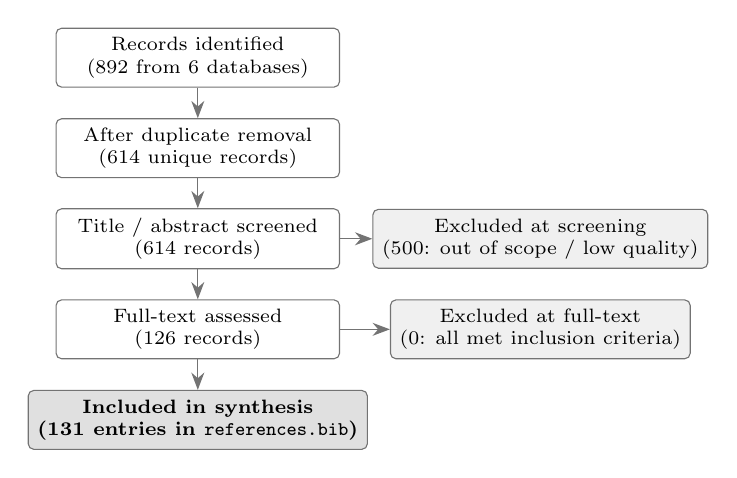
\begin{tikzpicture}[
  prisma/.style={draw=black!55, fill=white, rounded corners=2pt,
    minimum width=3.6cm, minimum height=0.72cm, align=center, font=\scriptsize},
  prismaem/.style={prisma, fill=black!6, minimum width=3.0cm, minimum height=0.58cm},
  arr/.style={-{Stealth[length=2.2mm]}, line width=0.45pt, draw=black!55}
]
  \node[prisma] (id) at (0,0) {Records identified\\(892 from 6 databases)};
  \node[prisma] (dedup) at (0,-1.15) {After duplicate removal\\(614 unique records)};
  \node[prisma] (screen) at (0,-2.3) {Title / abstract screened\\(614 records)};
  \node[prismaem] (excl1) at (4.35,-2.3) {Excluded at screening\\(500: out of scope / low quality)};
  \node[prisma] (full) at (0,-3.45) {Full-text assessed\\(126 records)};
  \node[prismaem] (excl2) at (4.35,-3.45) {Excluded at full-text\\(0: all met inclusion criteria)};
  \node[prisma, fill=black!12, font=\scriptsize\bfseries] (incl) at (0,-4.6)
    {Included in synthesis\\(131 entries in \texttt{references.bib})};
  \draw[arr] (id) -- (dedup);
  \draw[arr] (dedup) -- (screen);
  \draw[arr] (screen) -- (full);
  \draw[arr] (full) -- (incl);
  \draw[arr] (screen.east) -- (excl1.west);
  \draw[arr] (full.east) -- (excl2.west);
\end{tikzpicture}
\caption[PRISMA-style literature screening flow]{PRISMA-style literature screening flow for the 2017--2026 evidence base. Counts reflect the scoped CWB modules and inclusion criteria in this subsection; the full bibliography contains 131 synthesised entries.}
\label{fig:prisma-flow}
\end{figure}

\begin{table}[H]
\centering
\footnotesize
\setlength{\tabcolsep}{4pt}
\renewcommand{\arraystretch}{1.12}
\caption[Top-10 ranked literature sources]{Top-10 ranked literature sources from the PRISMA synthesis.}
\label{tab:lit-top10}
\resizebox{\textwidth}{!}{%
\begin{tabular}{@{}cp{4.2cm}p{7.4cm}@{}}
\toprule
\tableheadcolor
\tableheadfont \# & \tableheadfont Source / Module / Operationalized In & \tableheadfont Headline Finding \\
\midrule
1 & Werner et al.\ 2022 [1] · DeFi mechanics · Ch.~3 & DeFi lending is uniformly flat, pool-based, overcollateralized \\
\rowcolor{RowShade}
2 & Tan 2023 (IMF) [5] · CBDC \& hierarchy · Ch.~3 & Two-tier CBDC distribution (central bank $\to$ commercial banks $\to$ users); hierarchical infrastructure is the key design choice \\
3 & Palaiokrassas et al.\ 2024 [3] · Fraud detection · Sec.~\ref{sec:aiml-support} & Multi-chain ML on 54M tx, F1 0.76--0.85 with behavioral features \\
\rowcolor{RowShade}
4 & Adom et al.\ 2022 [4] · Explainable AI · Sec.~\ref{sec:aiml-support} & SHAP outperforms LIME on lending datasets \\
5 & Weber et al.\ 2019 / Elliptic [R24] · Graph fraud · Sec.~\ref{sec:gnn-extension} & Graph-structured fraud signal in BTC transactions \\
\rowcolor{RowShade}
6 & McMahan et al.\ 2017 / FedAvg [R25] · Federated learning · Sec.~\ref{sec:fl-fraud} & Privacy-preserving model averaging across institutions \\
7 & BIS WP 905 [R13] · Stablecoin risk · Secs.~\ref{sec:stablecoin-first}, \ref{sec:mica-compliance} & Algorithmic stablecoins unsuitable for EM DeFi; USDC/USDT recommended \\
\rowcolor{RowShade}
8 & Atzei et al.\ 2017 [7] · Smart contract security · Sec.~\ref{sec:defense-in-depth} & SoK of EVM attack vectors \\
9 & EU MiCA + GENIUS Act [R36, R38] · Regulation · Sec.~\ref{sec:mica-compliance} & Stablecoin issuer authorization, reserve disclosure \\
\rowcolor{RowShade}
10 & Bangladesh Bank SP2025-02 [R44] · MFI precedent · Sec.~\ref{sec:over-indebt} & Female-to-male account parity 49\%/49\% in 2025; 89\% BRAC loans to women \\
\bottomrule
\end{tabular}%
}
\end{table}

\section{Review of Existing Research}

The idea of the Crypto World Bank is designed based on the examination of peer-reviewed materials, institutional reports, and industry figures covering more than one sphere of direct interest to our architecture: decentralized lending and hierarchical institutional DeFi, smart contract security and formal verification, ML-based fraud detection and explainable AI, oracle-mediated risk analytics, group lending and microfinance literature, correspondent banking economics, retail payments and remittance rails, stablecoin regulation, institutional settlement rails (mBridge/Agora), and optional conversational interfaces (LLM/MCP).

\subsection{Decentralized Lending and DeFi Protocol Design}

To understand the gap this thesis addresses, it is necessary to be precise about what DeFi lending protocols actually do and where their structural limits lie. A DeFi lending protocol is a system of smart contracts that automates the deposit-funding and credit-allocation functions of a bank without requiring a licensed intermediary to hold assets or enforce rules. The contracts are deployed to a public blockchain, so any address in the world can deposit or borrow without permission, KYC gating, or a relationship with a traditional financial institution. Interest rates are set algorithmically by a utilization curve---as more of the pool is borrowed, rates rise to attract more depositors---and liquidations of undercollateralized positions are triggered automatically by price oracle updates.

This model produces several genuine innovations over traditional lending: settlement is atomic and near-instant; interest accrues per block rather than monthly; the entire loan book is publicly auditable in real time; and there is no loan officer capable of applying discriminatory judgment. However, the model also has structural limits that are directly relevant to this thesis. First, all participants are \textit{anonymous and fungible}: the protocol makes no distinction between a national bank with \$10~billion in assets and an individual retail borrower---both access the same pool under the same rules. Second, borrowing is universally \textit{over-collateralized}: since there is no identity layer and no recourse in default, protocols require collateral exceeding the loan value, which excludes the estimated 1.4~billion adults with no digital assets. Third, capital flows in \textit{one direction only}: depositors fund a pool and borrowers draw from it; there is no institutional hierarchy, no inter-tier capital allocation, and no mechanism for groups of entities to co-fund a single loan.

In their SoK paper, Werner et al.~[1] systematize DeFi protocol design and confirm that current lending markets are homogeneous, pool-based, and over-collateralized, with no institutional hierarchy---a gap which is directly addressed by this project. Their taxonomy demonstrates that no current DeFi system can represent multi-tier capital flow in the manner of development finance, establishing the design space this thesis enters.

Bastankhah et al.~[2] present a data-driven DeFi lending protocol with an adaptive dual fast/slow control architecture, demonstrating that dynamic interest rate adjustment outperforms the static utilization curves used by Aave and Compound~[59]. Their approach validates the algorithmic interest rate model adopted in the CWB's kinked-rate design (Section~\ref{sec:kinked-rate}).

Chen et al.~[46] introduce a multi-chain lending model that allocates lending activity across blockchain networks to improve throughput and reduce congestion. Their cross-chain settlement system validates the technical feasibility of executing lending protocols in heterogeneous blockchain settings, directly informing the CWB's multi-chain deployment approach on Ethereum and Polygon.

Yang and Cui~[47] present a DeFi lending protocol evaluation framework quantifying risk through utilization ratio stability, liquidation efficiency, and interest rate responsiveness. Their methodology provides a benchmark structure applicable to comparing the performance of the CWB's hierarchical lending layers against existing flat-pool protocols.

Hartmann and Hasan~[48] introduce a peer-to-peer blockchain lending framework that eliminates intermediary overhead through smart contract-mediated loan origination and repayment. Though single-tier in architecture, their gas analysis and on-chain identity management strategies inform the CWB's transaction cost optimization approach. Dao et al.~[60] demonstrate that credit scoring models can be adapted for DeFi lending environments, validating the feasibility of data-informed borrowing limits within decentralized protocols.

\subsection{Machine Learning for Blockchain Security}

Palaiokrassas et al.~[3] use machine learning on multichain DeFi fraud over 54~million transactions in 23 protocols which show a demonstration that the behavioral characteristics of DeFi enhance Neural Network and XGBoost classifiers to F1-scores of 0.76--0.85 versus 0.08 using transactional features only. Their finding that the behavioral features are superior to raw transaction data directly informs the planned feature engineering for the Random Forest fraud detection model.

The algorithm of unsupervised anomaly detection presented by Liu et al.~[6] is the Isolation Forest algorithm. The algorithm identifies anomalies using recursive partitioning of data, which assigns shorter distances to outliers. Isolation Forest is specified as the secondary detection model when labeled fraud data are limited, enabling detection of attack patterns not present in the training set.

Hasan et al.~[49] introduce blockchain and machine learning to detect fraud with the help of a privacy-protecting and adjustment-flexible incentive-based method. Their framework trains ML classifiers on encrypted transaction characteristics via federated learning, whereby the operators of the detection model never get to see the individual transaction data. Our future extensions of our AI/ML layer involve the privacy-preserving paradigm, in which the histories of client transactions should be confidential and at the same time allow system-wide fraud pattern recognition.

\subsection{Explainable AI in Financial Decision Systems}

Direct comparison of LIME and SHAP on loan approval is given by Adom et al.~[4], SHAP offers more consistent and in-depth feature attributions, which are found to be deeper via Shapley values whereas LIME provides quicker running time but less sure descriptions across repeated evaluations. Their comparison motivates the specification of SHAP as the primary explainability technique for loan risk measurement, trading off interpretability depth with regulatory compliance requirements.

Yuan~[56] use interpretable models that are based on SHAP on credit default assessment proving that SHAP feature attributions on Gradient Boosting and Random Forest classifiers are able to score over 0.92 with complete interpretability of individual predictions. Their approach to causing per-client risk explanations tells our intended credit risk dashboard, where the approvers of loans look at SHAP waterfall plots before lending decisions are made.

\subsection{Hierarchical Distribution and Development Finance}

Tan~[5] constructs an IMF model in which CBDCs use a two-tier distribution architecture (central bank $\to$ commercial banks $\to$ users) that parallels the CWB four-tier hierarchy. The paper shows that distributed digital-currency infrastructure can leverage existing institutional channels---informing the platform's hierarchical capital-flow design rather than a flat DeFi pool model.

The article by Asaduzzaman et al.~[54] examines blockchain in the microcredit industry, showing that smart contract-based loan management can reduce administrative overhead by up to 60\% compared to manual microfinance processes. This result validates the economic case for programmable group lending; microfinance geography citations inform module design only and do not define a deployment jurisdiction for this thesis.

The joint BIS report~[53] examines retail CBDC design requirements, identifying a two-level distribution model (central bank to commercial banks to end users) as the preferred architecture. Their analysis of interoperability between CBDC systems and existing payment infrastructure informs the planned dual-currency facility that bridges fiat and cryptocurrency within participating banks.

\subsection{Cross-Tier Capital Flows and Programmable Multi-Directional Lending}
\label{sec:lit-cross-tier}

While Tan~[5] and the BIS foundational CBDC report~[53] establish two-tier CBDC distribution as the prevailing institutional pattern, the academic and policy literature on \emph{multi-directional} capital coordination---same-tier interbank lending, upward surplus repatriation, and syndicated co-funding---within a programmable ledger remains sparse relative to settlement-only CBDC pilots.

Kiff et al.~[134] survey retail CBDC operating models and distinguish single-tier from multi-tier architectures in which the central bank issues CBDC but delegates wallet and payment services to supervised intermediaries---the institutional analogue of downward allocation with retained wholesale oversight. Bindseil~[133] analyses tiered CBDC remuneration as a mechanism to preserve bank intermediation while granting the public access to central-bank liabilities, informing the asymmetric upward/downward rate structure planned for the \texttt{UpwardDepositFacility} (Section~\ref{sec:upward-flow}). Auer and B\"{o}hme~[135] propose hybrid CBDC architectures that combine direct central-bank claims with intermediary-delivered payment services, paralleling the CWB pattern in which retail clients access credit only through Local Banks while reserve authority remains at Tier~1.

On programmable implementation, the New York Fed / BIS \textit{Project Pine} prototype~[131] demonstrates a hierarchy of smart contracts---facility factories, exchange contracts, and collateral pools---for central-bank market operations in tokenized wholesale markets. Although Project Pine targets monetary-policy implementation rather than development-finance lending, its layered contract-factory pattern validates encoding cross-contract dependencies (reserve checks, collateral eligibility, rate bounds) that the CWB \texttt{InterBankLendingPool} and \texttt{SyndicatedLoan} modules extend to multi-entity lending.

Dong, Qiu, and Xu~[132] model blockchain-enabled \emph{cross-tier direct financing} in a three-tier supply chain, showing that transparent ledger visibility enables capital to reach deep-tier, capital-constrained participants when traditional delegate financing fails---a structural parallel to downward allocation reaching retail clients who cannot access wholesale tiers directly. Together, these sources support the claim that hierarchical, multi-directional capital flows are established in policy and operations research but not yet composed into a single DeFi lending specification; the gap the CWB architecture addresses (Figure~\ref{fig:cross-tier-lending}).

\subsection{Group Lending and Microfinance Digitization}

The solidarity group lending model, pioneered by Grameen Bank and scaled by BRAC into one of the world's largest microfinance institutions, demonstrates that peer-monitored mutual liability can achieve repayment rates exceeding 95\% among borrowers with no individual collateral or formal credit history. These rates are attributable to social pressure mechanisms---weekly group meetings, field officer oversight, community reputation, and progressive loan eligibility---that are preventive in nature. The blockchain extension encodes mutual liability in programmable contract logic (multi-signature consent, on-chain group formation, automatic collateral pool claims), but cannot replicate the preventive social pressure that drives analogue MFI outcomes. The CWB \texttt{GroupLendingPool} module is specified at pre-thesis stage; on-chain repayment rates are expected to be lower initially until credit history accumulates. Güçük et al.~[61] provide a broader literature review of privacy and trust in blockchain-based microlending, reinforcing privacy-preserving mechanisms in the group lending architecture.

\subsection{Smart Contract Security and Governance}

Atzei et al.~[7] list Ethereum smart contract attack vectors such as reentrancy, access control vulnerabilities, and integer overflow. Their taxonomy informs the planned use of OpenZeppelin \texttt{ReentrancyGuard}, Solidity~0.8.20 overflow protection, and role-based access control modifiers. Their defense-in-depth strategy motivates combining security primitives with formal verification, static analysis (Slither), and symbolic execution (Mythril) in Phase~IV.

The article by Wang et al.~[50] introduces ContractWard which is an automated vulnerability detection system that uses machine learning classifiers (Random Forest, SVM, k-NN) to classify six types of smart contract vulnerabilities based on the features of bytecodes. ContractWard scores F1-reentrancy and F1-access control with 0.96 and 0.93 respectively, proving that security auditing using ML can be used to supplement traditional static analysis tools. Our proposed security verification pipeline will utilize the use of machine learning-based static analysis tools.

Liao et al.~[51] present SoliAudit, that is an integration of machine learning classification and vulnerability assessment of smart contracts fuzz testing. Their hybrid approach---using ML to first prioritize probable vulnerable code paths then target fuzz testing---reduces audit time by an estimated 70\% of that spent on manual review. SoliAudit's methodology informs the planned security audit plan on the specified three-contract core and its extensions toward the full modular architecture.

So et al.~[52] come up with VERISMART, an extremely accurate Ethereum safety verifier which employs constraint-based abstract interpretation to detect arithmetic overflow, division-by-zero and array out-of-bound errors. VERISMART achieves 98.4\% accuracy on benchmark data, but has zero false positives, so it is a candidate tool to formally verify our smart contract invariants (e.g., reserve ratio maintenance, cascading interest rate limits).

\subsection{AI Security Features for Blockchain Lending}

In addition to the planned fraud detection and anomaly identification pipeline, other AI-based security features can enhance the Crypto World Bank's resilience to evolving threats:

\begin{itemize}[noitemsep]
\item \textbf{Graph Neural Network (GNN) transaction analysis:} GNN-based models are able to analyze the graph structure of transaction to identify coordinated rings of fraud---groups of wallets which conspire to rig the borrowing limits or make circular lending patterns. A study by Palaiokrassas et al.~[3] proves that graph-based features are much superior to flat transaction features as an indicator of DeFi fraud detection.

\item \textbf{Federated learning for cross-bank fraud intelligence:} Hasan et al.~[49] demonstrate that federated learning allows the collaboration between several institutions to detect and train fraud models without distributing raw transaction information. Deploying federated learning of the Crypto World Bank's National and Local Banks would allow detecting threats system wide without compromising the privacy of the per-bank data.

\item \textbf{Reinforcement learning for adaptive interest rates (Future Work):} RL agents could dynamically modify interest rate parameters to match market conditions and utilization rates, decreasing the lag of manual parameter governance.

\item \textbf{Real-time smart contract monitoring:} ML-based monitoring agents (informed by ContractWard~[50] and SoliAudit~[51]) can continuously analyze incoming transactions for patterns matching known exploit signatures, triggering the platform's pause mechanism before significant losses occur.

\item \textbf{Natural language processing for income verification:} NLP models are able to extract and validate income information in uploaded documents, saving the bank officers the manual review load but not eliminating verification accuracy.
\end{itemize}

\subsection{Gas Cost Optimization and Layer~2 Scalability}

In DeFi, Kim and Kim~[55] examine the optimal approaches to minimization of gas fees, demonstrating that transaction batching, calldata compression, and tactical timing of on-chain operations can save 30--50\% of gas costs on Ethereum mainnet. Their findings support the planned deployment to Polygon zkEVM Cardona (sub-cent fees on testnet) and inform optimization strategies for any future mainnet deployment. Complicated multi-step operations (analogous to the four-tier loan lifecycle) benefit disproportionately from Layer~2 deployment due to multiplicative gas savings across sequential contract calls.

\subsection{Correspondent Banking and Cross-Border Settlement}

The Bank of International Settlement~[21] and Financial Stability Board~[33] have extensively documented the structural inefficiencies of the correspondent banking network. In the traditional model, the banks are required to have pre-funded nostro accounts in every currency corridor, establishing a world pool of idle capital which can not be put into effective productive lending. SWIFT settlements and respondent banks involves routing of messages using MT103 payment directions, screening of compliance at all intermediates, and settlement time extensions to two--five business days. According to the World Bank Migration and Development Brief~[26] it is stated that the cost of transferring \$200 on cross-border is 6.49\% on average, with Sub-Saharan African corridors averaging more than 8\%. Cerutti, Firat, and P\'{e}rez-Saiz~[144] model how digital-money cost reductions could raise cross-border volumes in high-cost remittance corridors, while Du, Huang, and Scharfstein~[138] compare correspondent-banking, fintech money-transmitter, and stablecoin ``sandwich'' rails with harmonized all-in cost measures---finding that on-chain legs can undercut legacy rails but remain dependent on fiat on/off-ramp depth at corridor endpoints. These results encourage our development of on-chain settlement with close to instant finality and sub-cent transaction costs on Layer~2 networks, while honestly scoping fiat conversion as a separate infrastructure layer (Section~\ref{sec:future-retail-payments}).

\subsection{Retail Payments, Remittance, and Fiat On/Off-Ramps}
\label{sec:lit-retail-payments}

Beyond institutional lending, a parallel literature examines whether stablecoin-denominated rails can support everyday retail flows---client-to-client remittance, merchant checkout, and cash-like deposit/withdrawal---under compliance constraints. This body of work is directly relevant to the \texttt{CurrentAccount}, \texttt{P2PTransfer}, and merchant-checkout modules scoped as post-MVT future work (Section~\ref{sec:future-retail-payments}).

Ante~[136] surveys 866 U.S.\ remittance users and finds that approximately 26\% have adopted stablecoins for cross-border transfers, with digital and financial literacy as significant adoption drivers and continuance tied to perceived usefulness---supporting the CWB design choice to gate retail transfers behind a tiered KYC ladder rather than open anonymous wallets. Du et al.~[138] document the dominant operational pattern: fiat $\to$ stablecoin $\to$ on-chain transfer $\to$ fiat off-ramp (the ``stablecoin sandwich''), showing that settlement speed gains are often negated where local off-ramp liquidity is thin---the binding constraint the planned PSP integration must address.

For merchant acceptance, Li et al.~[137] systematize stablecoin retail payments against card networks through the \textbf{CLEAR} framework (cost, legality, experience, architecture, reach), concluding that stablecoins offer programmable settlement and lower rail fees but externalize dispute resolution and consumer protection relative to Visa/Mastercard---a gap the CWB \texttt{InsuranceFund} and Local-Bank reconciliation workflow are intended to close in closed-loop form. Zhang et al.~[140] analytically model retailer adoption of stablecoin checkout with blockchain traceability, finding trade-offs between refund volatility and information disclosure; their results caution that merchant USDC acceptance without fiat auto-conversion may deter risk-averse consumers. Fr\"{o}hlich et al.~[139] evaluate a Lightning-network point-of-sale prototype and show that checkout friction concentrates at the on-ramp (acquiring crypto), not at tap-to-pay itself---informing the UX priority of fiat-funded \texttt{CurrentAccount} balances over raw wallet-to-wallet payment.

Platform-economy payment architectures offer the closest analogue to CWB's Local-Bank--sponsored retail model. Lin et al.~[141] propose \textit{SecurePay}, combining permissioned blockchain escrow with regulated money for buyer--merchant--platform settlement at $\approx$256~TPS, validating multi-intermediary payment flows rather than open DEX checkout. The BIS \textit{Project Sela}~[147] prototype similarly assigns compliance and customer-facing services to private intermediaries atop a central-bank-operated ledger---paralleling Tier~1 reserve authority with Local Bank retail distribution. Cimaszewski et al.~[146] blueprint DLT cross-border settlement with jurisdictional interconnection, reinforcing that P2P ledger transfer is only one layer of a compliant remittance stack.

Policy sources define the regulatory envelope. The CPMI report on stablecoin arrangements in cross-border payments~[142] identifies exchanges, custodial wallets, and PSPs as the primary on/off-ramps without which stablecoins cannot achieve domestic or global acceptance. BIS Papers No.~170~[143] analyses reserve transparency and digital-dollarisation risks. FATF virtual-asset guidance~[145] distinguishes \emph{unhosted-wallet} P2P (outside Travel Rule transmission) from \emph{platform-mediated} transfers where a VASP must collect originator and beneficiary data---the compliance model for CWB's KYC-gated \texttt{P2PTransfer} module under Local Bank sponsorship rather than permissionless public-wallet remittance.

Together, these sources establish that retail payment extensions are empirically and regulatorily \emph{studyable}, but that no prior work composes hierarchical development-finance lending with closed-loop, compliance-gated remittance, merchant checkout, and PSP-mediated ramps in a single four-tier architecture---the research gap Section~\ref{sec:future-retail-payments} addresses.

\subsection{Monetary Policy Distribution and Financial Inequality}

Recent empirical studies have reported the distributional impact of monetary policy on wealth inequality. A 2025 cross-country study spanning 49 nations (1999--2019) discovered that the relationship between central bank asset purchases programs and greater wealth inequality, whose outcomes are stronger in the distribution of wealth and long lasting~[34] than income inequality effects. The Federal Reserve's own 2025 contractionary monetary analysis based on the U.S. metropolitan tax data confirmed that policies harm the income of low income employees~[35]. These findings deliver economic incentive to the design principles of Crypto World Bank: transparent and algorithmically determined monetary parameters (interest rates, reserve ratios, supply rules) are encoded in smart contracts rather than set discretionally by opaque committees. On-chain transparency reduces \textit{price discrimination}---all borrowers at the same tier face the same utilization-driven interest rate, eliminating the ability of loan officers to charge higher rates to less-informed borrowers. This is a distinct mechanism from the Cantillon Effect (a macroeconomic phenomenon concerning newly created money benefiting first recipients); the Cantillon Effect does not apply to the CWB because USDC is 100\%-reserve backed and no new money supply is created by the platform's operations~[36].

\subsection{Real-World Asset Tokenization and Institutional DeFi}

The tokenization of real-world assets is an emerging convergence of traditional and decentralized finance. The Corda platform of R3 boasts of more than \$17~billion in tokenized real-world assets on its permissioned ledger as of September 2025, with institutional participants including HSBC and Bank of America~[37]. Centrifuge has deployed in eight blockchain networks of more than \$1~billion in tokenized institutional fund products~[38]. The World Bank is using blockchain on its own public chain side to track the disbursement of funds using its FundsChain program (based on Hyperledger Besu) which is flown on 13 projects in 10 countries and increases to 250 projects by mid-2026~[39]. These developments confirm the institutional interest of blockchain-based financial infrastructure and the viability of hierarchical fund distribution design models on distributed ledgers. This institutional adoption is continued in the Crypto World Bank's trajectory through carrying out not only fund tracking but total hierarchical lending system that has on-chain interest rates, reserves and credit assessment.

\subsection{Graph Neural Networks for Relational Fraud Detection}
\label{sec:lit-gnn}

Recent work has demonstrated that DeFi fraud is fundamentally a relational phenomenon: coordinated borrowing rings, sybil attacks, and flash-loan manipulation appear in the wallet-interaction graph, not in individual transaction features. Cheng~et~al.~(2024)~[R24], Chang et~al.~(2024)~[121], and the DeFiGuard graph-neural-network architecture~[R25] consistently outperform flat ML baselines on blockchain fraud, with reported detection above 70\% of illicit transactions at sub-1\% false-positive rates on the Elliptic dataset; Wang and Wang (2025) report similar advantages on cross-chain laundering~[R26]. This evidence motivates a Graph Neural Network (GNN) extension to the platform's Random-Forest fraud-detection layer, treated as an ablation isolating the marginal value of \textit{hierarchical tier-relationship edges} over flat wallet graphs---a question unanswered in the literature. The GNN extension is described in Section~\ref{sec:gnn-extension}.

\subsection{Federated Learning Across Banking Tiers}
\label{sec:lit-fl}

Hasan et~al.~(2022)~[49] introduced privacy-preserving fraud detection via federated learning on the blockchain. The PrivChain-AI study~[R27] in \textit{Nature Scientific Reports} (December~2025) demonstrates the same pattern with 94.7\% fraud-detection accuracy across multiple banks, while Abbassi et~al.~(2025)~[R28], FED-SPFD~[R29], and FedFraud~[125] document regulatory-grade FL for cross-border fraud intelligence. Cross-tier DeFi federated learning has not been studied; the Crypto World Bank's four-tier structure---where National and Local Banks are independent legal entities that cannot share raw transaction data---makes FedAvg + differential privacy architecturally appropriate: each Local Bank trains a local fraud model, parameter updates are aggregated at the National Bank tier, and no raw records leave the bank. The detailed FL pipeline is given in Section~\ref{sec:fl-fraud}.

\subsection{Stablecoin Regulation: MiCA and GENIUS Act}
\label{sec:lit-stablecoin-reg}

Two recent statutes reshape the legal context of any stablecoin-denominated lending platform. The EU Markets in Crypto-Assets (MiCA) Regulation, fully in effect from December~2024, requires authorized issuers, 1{:}1 reserve backing, and regular audits for electronic-money tokens---categories that directly cover USDC and USDT used at retail tiers of this platform~[R36, R37]. The United States GENIUS Act of July~2025 creates the first federal payment-stablecoin framework with similar reserve and disclosure obligations~[R38]. These statutes are read in this thesis not as obstacles but as the regulatory anchor that makes stablecoin-first design defensible (Section~\ref{sec:stablecoin-first}); the corresponding compliance mapping is presented in Section~\ref{sec:mica-compliance}.

\subsection{On-Chain Credit Passport and Soulbound Tokens}
\label{sec:lit-sbt}

Buterin, Hitzig, and Weyl~(2022)~[R30] introduce the concept of Soulbound Tokens (SBTs)---non-transferable ERC-style credentials that bind reputational data to an identity rather than to a tradable asset. For a multi-tier cryptocurrency exchange and financial services platform, SBTs provide a natural primitive for a portable on-chain credit passport: a client's successful repayment history at one Local Bank becomes a credential they can present to any other CWB Local Bank, and (with the schema fixed) to any external lending protocol that adopts the standard. MicroSave Consulting~(December~2025)~[R31] documents the microfinance sector's shift toward performance-based credit identity, providing literature support for the credit-passport design. The full credit-passport schema is in Section~\ref{sec:credit-passport}.

\subsection{Institutional DeFi Gap and the mBridge/Agora Landscape}
\label{sec:lit-institutional}

Sygnum Bank's February~2026 report \textit{Institutional DeFi in 2025}~[R21] documents the central gap that this thesis attempts to fill: DeFi protocols work technically, but pension-fund and endowment allocators do not participate until legal enforceability is resolved (Aave Arc held only $\approx$\$50\,k TVL despite permissioned architecture). The BIS mBridge platform~[R39] (China, Hong Kong, Thailand, UAE, Saudi Arabia) reached Minimum Viable Product status in mid-2024 and now settles real-value cross-border CBDC transactions, and the BIS / central-bank \textit{Project Agora}~[R40] explores tokenized bank deposits on a unified ledger. The IMF CBDC survey 2025 reports that 94\% of central banks are now engaged in CBDC research~[R32]. None of these initiatives implements a retail lending hierarchy: they are settlement rails. This positions the Crypto World Bank explicitly as the lending-layer \textit{specification} compatible with such institutional CBDC infrastructure rather than as a competitor to it.

\subsection{AI/ML Oracle and DeFi Fraud Literature (2024--2026)}
\label{sec:lit-ml-oracle}

Luo et al.~(2024) provide the most comprehensive survey of AI-powered fraud detection across the DeFi project lifecycle~[122]; CWB is positioned as a \textit{system instantiation} of that framework rather than a derivative survey. Caldarelli~(2025) surveys AI techniques applied to blockchain oracles and identify ML-score delivery for lending governance---not price feeds---as an under-researched interface~[123]. The BCCC-DeFiFraudTrans-2025 dataset (1,026,867 annotated transactions, 79 features) is introduced by York University BCCC~[108] and serves as the primary supervised training corpus (Section~\ref{sec:ml-workload}); Fazliani et al.~(2025) demonstrate semi-supervised DeFi fraud detection as a baseline the stacking approach should be compared against~[124]. For federated learning, Alhasawi et al.~(2025) report F1$=$0.90 on credit-card fraud with trust-aware aggregation~[125]---the direct baseline for the cross-tier DeFi FL extension (Section~\ref{sec:fl-fraud}).

\subsection{LLMs in Finance and Hallucination Risk}
\label{sec:lit-llm}

The optional CWB conversational add-on is specified to use an 8B-parameter open-weight LLM with QLoRA fine-tuning, RAG over the platform's policy and contract documents, and an explicit refusal layer for regulated questions. The LLM-in-finance literature~[R33, R34, R35] gives both the design rationale and the necessary cautions: Morgan Stanley's GPT-based equity-analysis assistant achieved a reported 50\% reduction in analyst time, McKinsey estimates LLMs can cut back-office costs by 40\%, but the 2025 LLM-vulnerability-in-finance corpus~[R35] documents specific regulatory-hallucination failure modes when LLMs are asked compliance questions without RLHF from domain experts. The evaluation methodology in Section~\ref{sec:llm-eval} includes a red-teaming protocol for adversarial financial prompts directly motivated by this work.

\section{Literature Review Summary}

The most important reviewed works with their methodologies, key findings, and relevance to our project are presented in Table~\ref{tab:lit-summary}, in the form of literature table suggested by Michigan State University Libraries~[23].

\begin{table}[H]
\centering
\footnotesize
\setlength{\tabcolsep}{4pt}
\renewcommand{\arraystretch}{1.12}
\caption[Literature review summary (Part A)]{Literature review summary (Part A): DeFi lending, fraud detection, and XAI.}
\resizebox{\textwidth}{!}{%
\begin{tabular}{@{}>{\raggedright\arraybackslash}p{3.4cm}>{\raggedright\arraybackslash}p{3.0cm}>{\raggedright\arraybackslash}p{3.8cm}>{\raggedright\arraybackslash}p{3.5cm}@{}}
\toprule
\tableheadcolor
\tableheadfont Author \& Focus & \tableheadfont Methodology & \tableheadfont Key Findings & \tableheadfont Relevance to Our Project \\
\midrule
Palaiokrassas et al.\ (2024) [3] · DeFi fraud detection & XGBoost, NN classifiers on 54M+ multi-chain transactions & F1: 0.76--0.85 vs.\ 0.08 with features alone & Informs Random Forest fraud modeling \\
Adom et al.\ (2022) [4] · XAI in loan approval & LIME / SHAP comparison on lending datasets & SHAP provides deeper, more consistent explainability; LIME is faster & Justifies SHAP as our primary explainability method \\
Tan (2023) [5] · CBDC hierarchical distribution & Model for developing nations & Two-tier CBDC distribution (central bank $\to$ commercial banks $\to$ users); hierarchical infrastructure is the decisive design choice & Informs four-tier architecture and dual-currency facility \\
Liu et al.\ (2008) [6] · Anomaly detection & Isolation Forest on synthetic and real datasets & Isolation via recursive partitioning; shorter paths & Specified as secondary unsupervised detection for wallet behaviour \\
Atzei et al.\ (2017) [7] · Smart contract security & SoK of Ethereum attack vectors & Over-reliance, access control vulnerabilities & Directly informs our security primitives and planned formal verification \\
\bottomrule
\end{tabular}%
}
\TableScreenshotEnd[tab:lit-summary]{Literature Review Summary (Part 1): DeFi Lending and Hierarchical Architecture}
\end{table}

\vspace{2pt}
\noindent\textit{\small Of the works reviewed, none model a four-tier hierarchical lending structure, confirming the architectural novelty of this project. The synthesis shows that DeFi and institutional finance have developed in parallel without converging on a governance-aware, multi-tier design.}

\begin{table}[H]
\centering
\footnotesize
\setlength{\tabcolsep}{4pt}
\renewcommand{\arraystretch}{1.12}
\caption[Literature review summary (Part B)]{Literature review summary (Part B): DeFi protocol systematisation and adaptive lending.}
\resizebox{\textwidth}{!}{%
\begin{tabular}{@{}>{\raggedright\arraybackslash}p{3.4cm}>{\raggedright\arraybackslash}p{3.0cm}>{\raggedright\arraybackslash}p{3.8cm}>{\raggedright\arraybackslash}p{3.5cm}@{}}
\toprule
\tableheadcolor
\tableheadfont Author \& Focus & \tableheadfont Methodology & \tableheadfont Key Findings & \tableheadfont Relevance to Our Project \\
\midrule
Werner et al.\ (2022) [1] · DeFi protocol systematisation & SoK survey of 12+ DeFi protocol categories & Lending platforms are uniformly pool-based and overcollateralised; no institutional hierarchy exists & Identifies the core gap our four-tier architecture addresses \\
Bastankhah et al.\ (2024) [2] · Adaptive DeFi lending & Dual fast/slow control; simulation on historical data & Dynamic rate adjustment outperforms static utilisation curves & Validates algorithmic lending parameter optimisation \\
\bottomrule
\end{tabular}%
}
\TableScreenshotEnd{Literature Review Summary (Part 2): Governance, Settlement, and Institutional Adoption}
\end{table}

\vspace{2pt}
\noindent\textit{\small This continuation extends coverage to governance, settlement, and institutional blockchain adoption. The key observation is that enabling infrastructure (Layer~2 networks, oracle pricing, EVM tooling) is mature, while the specific hierarchical banking architecture remains architecturally unexplored.}

\begin{table}[H]
\centering
\footnotesize
\setlength{\tabcolsep}{4pt}
\renewcommand{\arraystretch}{1.12}
\caption[Literature review summary (Part C)]{Literature review summary (Part C): blockchain P2P lending, privacy-preserving ML, and smart contract auditing.}
\resizebox{\textwidth}{!}{%
\begin{tabular}{@{}>{\raggedright\arraybackslash}p{3.4cm}>{\raggedright\arraybackslash}p{3.0cm}>{\raggedright\arraybackslash}p{3.8cm}>{\raggedright\arraybackslash}p{3.5cm}@{}}
\toprule
\tableheadcolor
\tableheadfont Author \& Focus & \tableheadfont Methodology & \tableheadfont Key Findings & \tableheadfont Relevance to Our Project \\
\midrule
Hartmann and Hasan (2021) [48] · Blockchain P2P lending & Smart contract-mediated loan origination framework & Eliminates intermediary overhead; gas cost minimisation analysis & Informs four-tier architecture for peer-to-peer lending \\
Hasan et al.\ (2022) [49] · Privacy-preserving fraud detection & Federated learning on encrypted blockchain features & ML achieves comparable accuracy to centralised models & Informs future privacy-preserving fraud detection extensions \\
Wang et al.\ (2020) [50] · Smart contract vulnerability detection & ML classifiers on bytecode features & F1: 0.96 for access control; 0.93 for data leakage & Supports our planned security verification models \\
Liao et al.\ (2019) [51] · Smart contract audit automation & Hybrid classification + fuzz testing & Reduces audit time by 70\% vs.\ manual review & Informs our security audit strategy for three-contract architecture \\
\bottomrule
\end{tabular}%
}
\TableScreenshotEnd{Literature Review Summary (Part 3): Cross-Border Settlement and Security Tooling}
\end{table}

\vspace{2pt}
\noindent\textit{\small This continuation captures empirical and systems findings on cross-border settlement and security tooling, supporting the claim that Layer~2 deployment and hybrid ML-static analysis pipelines substantially reduce feasibility risk for an academic prototype.}

\begin{table}[H]
\centering
\footnotesize
\setlength{\tabcolsep}{4pt}
\renewcommand{\arraystretch}{1.12}
\caption[Literature review summary (Part D)]{Literature review summary (Part D): CBDC design, cross-border settlement, and multi-chain DeFi.}
\resizebox{\textwidth}{!}{%
\begin{tabular}{@{}>{\raggedright\arraybackslash}p{3.4cm}>{\raggedright\arraybackslash}p{3.0cm}>{\raggedright\arraybackslash}p{3.8cm}>{\raggedright\arraybackslash}p{3.5cm}@{}}
\toprule
\tableheadcolor
\tableheadfont Author \& Focus & \tableheadfont Methodology & \tableheadfont Key Findings & \tableheadfont Relevance to Our Project \\
\midrule
BIS et al.\ (2020) [53] · CBDC design requirements & Analysis of retail CBDC distribution architecture & Two-tier model preferred; interoperability challenges identified & Informs dual-currency facility design \\
Kiff et al.\ (2020) [134] · CBDC operating models & IMF survey of retail CBDC architectures & Multi-tier models delegate distribution to supervised intermediaries & Supports four-tier wholesale-to-retail capital path \\
Bindseil (2020) [133] · Tiered CBDC remuneration & ECB policy analysis of two-tier CBDC rates & Tiered rates preserve bank intermediation; control disintermediation risk & Informs upward/downward asymmetric rate spread \\
Dong et al.\ (2023) [132] · Cross-tier supply-chain finance & Three-tier game-theoretic MSOM model & Blockchain cross-tier direct financing reaches capital-constrained deep tiers & Parallel to downward client lending without wholesale bypass \\
Project Pine (2025) [131] · Hierarchical smart contracts & NY Fed / BIS tokenized policy toolkit prototype & Factory-to-facility contract hierarchy for reserves and collateral & Validates layered contract design for \texttt{IBLP} / \texttt{SyndicatedLoan} \\
BIS/FSB [21] · Cross-border settlement infrastructure & Analysis of cross-border payment costs and capital trapped in nostro accounts & 2--5 days avg.\ settlement; \$42/transfer avg.\ cost & Motivates four-tier settlement with near-instant finality \\
Beyer et al.\ (2025) [34] · Monetary policy and inequality & Cross-country analysis (1999--2019) & QE increases wealth inequality; effects more persistent than monetary parameters & Motivates transparent, algorithmic monetary parameters \\
World Bank (2025) [39] · Blockchain for development finance & Pilot on 13 projects, 10 countries & Blockchain tracking reduces reporting burden for fund distribution & Supports our planned multi-chain deployment strategy \\
\bottomrule
\end{tabular}%
}
\TableScreenshotEnd{Literature Review Summary (Part 4): Risk Monitoring and AI/ML in Finance}
\end{table}

\vspace{2pt}
\noindent\textit{\small This block summarizes works informing the platform's risk and monitoring approach. The synthesis justifies the choice of lightweight, auditable ML components rather than opaque deep learning models, prioritizing regulatory interpretability over raw detection performance.}

\begin{table}[H]
\centering
\footnotesize
\setlength{\tabcolsep}{4pt}
\renewcommand{\arraystretch}{1.12}
\caption[Literature review summary (Part E)]{Literature review summary (Part E): multi-chain DeFi, smart microfinance, gas optimisation, and SHAP-based credit models.}
\resizebox{\textwidth}{!}{%
\begin{tabular}{@{}>{\raggedright\arraybackslash}p{3.4cm}>{\raggedright\arraybackslash}p{3.0cm}>{\raggedright\arraybackslash}p{3.8cm}>{\raggedright\arraybackslash}p{3.5cm}@{}}
\toprule
\tableheadcolor
\tableheadfont Author \& Focus & \tableheadfont Methodology & \tableheadfont Key Findings & \tableheadfont Relevance to Our Project \\
\midrule
Chen et al.\ (2024) [46] · Multi-chain DeFi lending & Cross-chain model design and implementation & Multi-chain distribution improves throughput and reduces congestion & Supports our planned multi-chain deployment strategy \\
Yang and Cui (2023) [47] · DeFi lending protocol evaluation & Quantitative risk metrics for lending protocol assessment & Utilisation ratio, liquidation efficiency, and reserve responsiveness as key metrics & Provides benchmarks for evaluating our hierarchical tiers \\
Asaduzzaman et al.\ (2020) [54] · Smart micro-credit (MFI literature) & Smart contract-based microfinance & Reduces admin overhead by 60\% vs.\ manual processes & Informs \texttt{GroupLendingPool} economic case \\
Kim and Kim (2024) [55] · DeFi gas fee optimisation & Transaction batching and calldata compression analysis & Gas savings of 30--50\% through optimisation strategies & Validates Layer~2 deployment and mainnet optimisation \\
Yuan (2024) [56] · SHAP-based credit default models & SHAP, Random Forest, and Gradient Boosting classifiers & AUC above 0.92 with full interpretability & Informs per-client risk explanation methodology \\
\bottomrule
\end{tabular}%
}
\TableScreenshotEnd{Literature Review Summary (Part 5): Institutional Adoption and MFI Literature}
\end{table}

\vspace{2pt}
\noindent\textit{\small This final block closes the synthesis with institutional and microfinance-literature sources. The combined evidence supports increasing institutional blockchain adoption alongside persistent gaps in hierarchical, governance-aware lending---matching the platform's institutional-first, multi-tier scope.}

\begin{table}[H]
\centering
\footnotesize
\setlength{\tabcolsep}{4pt}
\renewcommand{\arraystretch}{1.12}
\caption[Literature review summary (Part F)]{Literature review summary (Part F): retail payments, remittance, merchant checkout, and fiat on/off-ramps.}
\resizebox{\textwidth}{!}{%
\begin{tabular}{@{}>{\raggedright\arraybackslash}p{3.4cm}>{\raggedright\arraybackslash}p{3.0cm}>{\raggedright\arraybackslash}p{3.8cm}>{\raggedright\arraybackslash}p{3.5cm}@{}}
\toprule
\tableheadcolor
\tableheadfont Author \& Focus & \tableheadfont Methodology & \tableheadfont Key Findings & \tableheadfont Relevance to Our Project \\
\midrule
Ante (2025) [136] · Stablecoin remittance adoption & Survey ($n{=}866$) of U.S.\ remittance users & 26\% stablecoin adoption; literacy drives uptake; continuance tied to usefulness & Informs KYC ladder and UX for \texttt{P2PTransfer} \\
Du et al.\ (2026) [138] · Competing payment rails & Harmonized all-in cost comparison across corridors & Stablecoin sandwich can undercut banks/MTOs; off-ramp depth is binding & Motivates PSP on/off-ramp future work \\
Li et al.\ (2026) [137] · Stablecoin retail payments SoK & CLEAR framework vs.\ card networks & Closed-loop / cross-border advantage; weak open-loop dispute recourse & Frames merchant checkout and \texttt{InsuranceFund} design \\
Zhang et al.\ (2024) [140] · Retail stablecoin checkout & Analytical operations model & Stablecoin refunds create consumer volatility disutility & Supports fiat-display \texttt{FXModule} and auto-conversion \\
Fr\"{o}hlich et al.\ (2022) [139] · Crypto POS usability & Mixed-methods Lightning checkout study & Friction at on-ramp, not tap-to-pay & Prioritises fiat-funded \texttt{CurrentAccount} balances \\
Lin et al.\ (2025) [141] · Platform-economy payments & Permissioned chain + regulated money prototype & $\approx$256~TPS; multi-intermediary escrow & Parallel to Local-Bank--sponsored merchant flows \\
CPMI / BIS [142,143] · Stablecoin policy & Cross-border and monetary-system analysis & On/off-ramps gate acceptance; reserve transparency critical & Regulatory anchor for ramp integration \\
FATF (2021) [145] · VASP / P2P guidance & Risk-based AML standards for virtual assets & Platform-mediated transfers require originator data; pure unhosted P2P out of scope & Compliance model for sponsored \texttt{P2PTransfer} \\
\bottomrule
\end{tabular}%
}
\TableScreenshotEnd{Literature Review Summary (Part 6): Retail Payments and Remittance Rails}
\end{table}

\vspace{2pt}
\noindent\textit{\small This block grounds the post-MVT retail-payment roadmap (Section~\ref{sec:future-retail-payments}) in peer-reviewed and policy literature. The synthesis shows these features are empirically studyable but not yet integrated with hierarchical development-finance lending.}


\section{Comparative Protocol Analysis}
\label{sec:comparative-protocol}

The literature survey above reveals that no existing DeFi protocol combines multi-tier institutional hierarchy with AI-assisted governance and compliance-aware identity. Table~\ref{tab:protocol-comparison} provides a structured comparison of the Crypto World Bank against representative existing protocols on eleven architectural dimensions.

\begin{table}[H]
\centering
\footnotesize
\setlength{\tabcolsep}{3pt}
\resizebox{\textwidth}{!}{%
\begin{tabular}{@{}p{3.4cm}*{6}{>{\centering\arraybackslash}p{1.35cm}}@{}}
\toprule
\tableheadcolor
\tableheadfont Feature & \tableheadfont Aave & \tableheadfont Comp. & \tableheadfont Maker & \tableheadfont Maple & \tableheadfont Gfinch & \tableheadfont CWB \\
\midrule
Institutional hierarchy & \tmarkNo{} & \tmarkNo{} & \tmarkNo{} & \tmarkNo{} & \tmarkNo{} & \tmarkPlanned{} \\
\rowcolor{RowShade}
Cross-tier capital flow & \tmarkNo{} & \tmarkNo{} & \tmarkNo{} & \tmarkNo{} & \tmarkNo{} & \tmarkPartial{} \\
Same-tier interbank lending & \tmarkNo{} & \tmarkNo{} & \tmarkNo{} & \tmarkNo{} & \tmarkNo{} & \tmarkPartial{} \\
\rowcolor{RowShade}
Syndicated / co-lending & \tmarkNo{} & \tmarkNo{} & \tmarkNo{} & Part. & Part. & \tmarkPartial{} \\
Upward capital repatriation & \tmarkNo{} & \tmarkNo{} & \tmarkNo{} & \tmarkNo{} & \tmarkNo{} & \tmarkPartial{} \\
\rowcolor{RowShade}
Solidarity group lending & \tmarkNo{} & \tmarkNo{} & \tmarkNo{} & \tmarkNo{} & Part. & \tmarkPlanned{} \\
AI/ML fraud detection & \tmarkNo{} & \tmarkNo{} & \tmarkNo{} & Man. & Man. & \tmarkPlanned{} \\
\rowcolor{RowShade}
SHAP explainability & \tmarkNo{} & \tmarkNo{} & \tmarkNo{} & \tmarkNo{} & \tmarkNo{} & \tmarkPlanned{} \\
ZKP KYC compliance & \tmarkNo{} & \tmarkNo{} & \tmarkNo{} & \tmarkNo{} & \tmarkNo{} & \tmarkPlanned{} \\
\rowcolor{RowShade}
Kinked interest rate curve & \tmarkDone{} & \tmarkDone{} & Gov. & \tmarkDone{} & \tmarkNo{} & \tmarkPartial{} \\
Role-based access control & Part. & Part. & Gov. & \tmarkDone{} & Part. & \tmarkPlanned{} \\
\rowcolor{RowShade}
Institutional / L2 focus & \tmarkNo{} & \tmarkNo{} & \tmarkNo{} & \tmarkDone{} & Part. & \tmarkPlanned{} \\
TVL / Status (2026) & \$26B & \$1.4B & \$10B & \$2.6B & \$680M & Planning \\
\bottomrule
\end{tabular}%
}
\caption[Protocol comparison on eleven architectural dimensions]{Protocol comparison on eleven architectural dimensions. Competitor columns reflect publicly documented protocol capabilities (2026); CWB columns reflect pre-thesis specification status.}
\label{tab:protocol-comparison}
\end{table}

This comparison directly answers RQ1: no existing protocol simultaneously enforces a four-tier reserve-ratio hierarchy, oracle-mediated explainable ML governance, and programmable mutual-liability group lending. While Aave~v3 implements risk-parameterized sub-markets (Isolation Mode, Efficiency Mode) and Compound~v3 deploys separate Comet markets, these mechanisms differentiate risk parameters for different assets within a single-tier pool---they do not model institutional relationships, cross-tier governance, or inter-bank lending flows. Maple Finance, Goldfinch, and Morpho~V2 approach institutional credit from flatter market-structure angles~[117,118]; none mirrors multilateral development-finance capital allocation. The Crypto World Bank's compound novelty claim (Section~\ref{sec:research-contribution}) holds when stated precisely across all three axes.

\paragraph{Note on ERC-3643 (T-REX) for institutional-tier permissioning.}
The institutional tiers (Tiers~1--3) use the bespoke RBAC described in Section~\ref{sec:defense-in-depth} for transfer-level access control.  ERC-3643 (the T-REX standard for permissioned, compliance-gated token transfers) and ERC-4626 for tokenized vaults are gaining adoption as standards that ensure tokenized assets can plug and play across platforms without custom integrations~[R46].  ERC-3643 is specifically designed for regulated institutional token transfers where KYC and AML checks gate individual token movements at the token contract level, rather than at the application layer.  The platform's current RBAC serves the same functional purpose: role gates on every state-mutating function enforce that only KYC-verified, role-holding addresses can transfer institutional-tier assets.  A production deployment operating under MiCA~[R36] or equivalent regulated-asset frameworks would evaluate full ERC-3643 compliance as the path to interoperability with other regulated tokenized-asset platforms; the architecture is designed to accommodate this migration because the RBAC role structure maps directly onto the ERC-3643 identity registry model.  This note is recorded here rather than as a Future Work item so that examiners can identify the deliberate design alignment.

\paragraph{Positioning against failed centralized exchanges.}
Centralized cryptocurrency exchanges such as FTX (defunct, 2022) demonstrate the catastrophic consequence of opaque reserve management: an \$8~billion client-fund shortfall was discovered only at the point of bankruptcy, having been concealed through commingling of client deposits with proprietary trading activity by its affiliated trading firm Alameda Research. FTX halted withdrawals and filed for bankruptcy within three days. The structural cause was centralized custody with no on-chain proof of reserves, no separation between customer funds and operating capital, and no real-time verifiability of solvency. The Crypto World Bank's on-chain reserve architecture is designed as a structural response to this class of failure: every tier's reserve ratio is an enforced smart contract invariant, readable by any participant in real time without trust in any third-party attestation. This design property---on-chain Proof of Reserves by construction---is increasingly recognized as the non-negotiable foundation of trustworthy crypto-financial infrastructure, and the Crypto World Bank implements it at the institutional tier level rather than the exchange-account level. The platform's purpose is also structurally distinct from FTX: it targets institutional and retail banking (savings, credit, interbank lending)---not speculative trading, derivatives, or leveraged tokens---and its four-tier institutional hierarchy mirrors multilateral development finance rather than a flat exchange order book. DeFi naturally provides on-chain transparency, self-custody, and governance---precisely the properties whose absence destroyed FTX.

\subsection{Literature Synthesis}

The literature synthesis above directly informs six architectural decisions in this work: (1) Gudgeon et al.'s~(2020)~[R3] empirical finding that utilization above 90\% causes liquidity crises motivates the kinked interest rate model in Section~\ref{sec:kinked-rate}; (2) Piper et al.'s~(2025)~[R8] ZKP permissioning framework provides the technical foundation for the compliance pathway in Section~\ref{sec:identity}; (3) Tan~(2023)~[5], the BIS foundational CBDC report~[53], Kiff et al.~[134], and Auer and B\"{o}hme~[135] on hierarchical and hybrid CBDC distribution inform the four-tier capital-flow model and client-via-Local-Bank entry path; (4) Bindseil~[133], Project Pine~[131], and Dong et al.~[132] on tiered remuneration, hierarchical smart contracts, and cross-tier direct financing inform the multi-directional lending modules in Section~\ref{sec:cross-tier-lending}; (5) Asaduzzaman et al.'s~(2020)~[54] on blockchain microcredit provides prior art for the programmable \texttt{GroupLendingPool} module (literature precedent, not a deployment jurisdiction claim); and (6) Ante~[136], Du et al.~[138], Li et al.~[137], Lin et al.~[141], CPMI~[142], and FATF~[145] on stablecoin remittance, competing payment rails, retail-payment architecture, platform-economy settlement, and VASP-mediated compliance inform the post-MVT retail stack (\texttt{CurrentAccount}, \texttt{P2PTransfer}, merchant checkout, PSP ramps) in Section~\ref{sec:future-retail-payments}.

\subsection{Agent Harness Engineering and Production Safety}
\label{sec:harness-lit}

A parallel research stream has documented prompt injection as the dominant
vulnerability in production banking agents. Alizadeh et~al.~[R53]
demonstrate that income document uploads and language preference fields in
banking tool-calling agents are viable injection vectors for personal data
exfiltration --- the same fields present in the CWB context assembly pipeline.
The OWASP Top~10 for LLM Applications~[R54] classifies LLM01 (Prompt
Injection) as the highest-priority threat in agentic financial systems, providing
an authoritative standard against which the CWB scanning middleware can be
evaluated.

\section{Summary of Key Findings}

The following summarized findings are obtained in the literature review and are directly informative to our design:

\begin{itemize}[noitemsep]
\item \textbf{DeFi lending is structurally flat.} Available protocols (Aave, Compound, MakerDAO) operate pool-based or over-collateralized models with total value locked exceeding \$55~billion~[13]. Institutional hierarchy has no comparable protocol models to development finance. CBDC research~[5] ascertains that tiered distribution is a workable institutional design pattern.
\item \textbf{Correspondent banking is inefficient in structure.} Cross-border settlement spends two to five days at average costs of \$42 per transaction~[25]. The system traps important capital lying idle in nostro/vostro accounts~[24], and remittance fees are estimated to consume between \$48--56~billion a year~[26]. Cerutti et al.~[144] and Du et al.~[138] show that digital-money and stablecoin rails can compress corridor costs but remain constrained by fiat on/off-ramp infrastructure---motivating the phased retail-payment roadmap (Sections~\ref{sec:lit-retail-payments},~\ref{sec:future-retail-payments}).
\item \textbf{Retail stablecoin payments are studyable but not open-loop card substitutes.} Li et al.~[137] find stablecoins advantaged in closed-loop and cross-border contexts; Zhang et al.~[140] and Fr\"{o}hlich et al.~[139] highlight refund volatility and on-ramp friction. Platform-mediated models (Lin et al.~[141]; BIS Project Sela~[147]) validate Local-Bank--sponsored checkout rather than permissionless merchant wallets.
\item \textbf{ML enhances fraud detection in blockchain.} DeFi-specific behavioral features significantly work well as compared to transactional features (F1: 0.76--0.85 vs.\ 0.08~[3]). The Isolation Forest~[6] allows unsupervised detection in which labeled data is scarce.
\item \textbf{SHAP is explainable by regulators.} SHAP offers greater consistency and is better than the LIME in loan approval systems~[4] in meeting prudential demands on open-minded automated decision-making.
\item \textbf{Layered defense is needed in smart contract security.} Reentrancy, overflow, and vulnerabilities to access control are well documented~[7]. ML-based vulnerability detection achieves F1-scores of above 0.93~[50], and hybrid ML-fuzz methods reduce audit time by 70\%~[51]. Verification tools are formal, i.e., VERISMART achieves 98.4\% precision~[52]. Automated primitives used with OpenZeppelin are recommended for production deployments to be verified.
\item \textbf{Monetary policy leads to distributional inequality.} Cross-country evidence~[34] and Federal Reserve research~[35] confirm that quantitative easing disproportionately favors asset holders, and workers of lower income cover the expenses of both inflation and consequent tightening. Transparent, algorithmic monetary parameters can decrease this informational asymmetry.
\item \textbf{The use of blockchains in institutions is gaining momentum.} The World Bank's FundsChain~[39], tokenized assets of R3 Corda worth \$17~billion~[37], and JPMorgan Kinexys settling multi-billion dollars per day~[40] reflect the fact that financial institutions are actively implementing blockchain on settlement, funds tracking, and asset tokenization.
\item \textbf{Microfinance literature informs group lending design.} Global unbanked statistics~[14] and mobile-money adoption studies motivate hierarchical intermediation in development finance. Blockchain-based microcredit research shows up to 60\% reduction in administrative overhead~[54], supporting the economic case for on-chain \texttt{GroupLendingPool} specification.
\item \textbf{Multi-chain lending enhances scalability.} Cross-chain lending models~[46] and Layer~2 gas optimization strategies~[55] prove the fact that the lending is distributed when operating on several networks, decreasing congestion and transaction costs by 30--50\%.
\item \textbf{ML can be used to detect cross-institutional fraud using privacy preserving ML.} Federated learning methods~[49] are such that enable several lending institutions to cooperate and learn fraud detection models in a non-intrusive manner, i.e. no individual transaction data is exposed, resolving the conflict between institution-wide security and data privacy.

\item \textbf{Group lending reduces default risk in analogue MFIs.} Microfinance research from BRAC, Grameen Bank, and ASA consistently reports repayment rates above 95\% in solidarity group structures~[54]. On-chain enforcement of mutual liability has not been studied in the academic literature, representing an open research gap that this specification begins to address.

\item \textbf{Sustainable microfinance requires deposit-funded lending.} Literature on sustainable microfinance institutions consistently shows that deposit-funded lending rather than donor-funded or externally capitalized models is the only economically viable approach at scale. The platform's banking product suite is designed to close this loop by mobilizing retail savings at the Local Bank tier to partially fund the lending pool.
\end{itemize}

The results explain why we have a four-tier architecture, AI/ML integration (Random Forest, Isolation Forest, SHAP), cross-tier lending structure, governance structure, and planned security verification pipeline.


%% CHAPTER 3: SYSTEM ARCHITECTURE AND DESIGN
\chapter{System Architecture and Design}

\section{Prototype Scope}
\label{sec:prototype-scope}

\begin{table}[H]
\centering
\caption[Prototype scope and implementation status]{Prototype scope: specification vs.\ planned implementation status (pre-thesis design record only; no live public deployment).}
\label{tab:prototype-scope}
\footnotesize
\renewcommand{\arraystretch}{0.88}
\setlength{\tabcolsep}{3pt}
\begin{tabular}{@{}p{7.1cm}>{\raggedleft\arraybackslash}p{5.9cm}@{}}
\toprule
\tableheadcolor
\tableheadfont Feature & \tableheadfont Status \\
\midrule
Four-tier role system (RBAC) & \tmarkPartial{} Specified \\
\rowcolor{RowShade}
World Bank Reserve contract (Tier~1) & \tmarkPartial{} Specified (Phase~I) \\
Tier~2 National Bank contracts & \tmarkPartial{} Specified (Phase~I) \\
\rowcolor{RowShade}
Tier~3 Local Bank contracts & \tmarkPartial{} Specified (Phase~I) \\
Cross-tier fund transfer & \tmarkPlanned{} Planned (Phase~II) \\
\rowcolor{RowShade}
Loan request / approval workflow & \tmarkPartial{} Specified (Phase~II) \\
Installment EMI auto-generation & \tmarkPlanned{} Planned (Phase~II) \\
\rowcolor{RowShade}
SavingsVault contract & \tmarkPlanned{} Planned (Phase~II) \\
FixedDeposit contract & \tmarkPlanned{} Planned (Phase~II) \\
\rowcolor{RowShade}
GroupLendingPool contract & \tmarkPlanned{} Planned (Phase~II) \\
InterBankLendingPool & \tmarkPlanned{} Planned (Phase~II) \\
\rowcolor{RowShade}
AI/ML fraud detection (Random Forest) & \tmarkPlanned{} Planned (Phase~III) \\
SHAP + anomaly explainability & \tmarkPlanned{} Planned (Phase~III) \\
\rowcolor{RowShade}
Oracle integration (Chainlink Functions) & \tmarkPlanned{} Planned (Phase~III) \\
ZKP KYC compliance layer & \tmarkPlanned{} Planned (Phase~IV) \\
\rowcolor{RowShade}
Testnet deployment (Polygon zkEVM Cardona) & \tmarkPlanned{} Planned (Phase~IV) \\
AI Agent / MCP tool server (17 tools) & \tmarkPlanned{} Optional (Phase~III--IV) \\
\rowcolor{RowShade}
EIP-7702 session key management & \tmarkPlanned{} Optional (Phase~III) \\
Authority Brief UI (SHAP for approvers) & \tmarkPlanned{} Planned (Phase~III) \\
\rowcolor{RowShade}
Chainlink Automation (installment triggers) & \tmarkPlanned{} Planned (Phase~II) \\
Chainlink Proof of Reserve & \tmarkPlanned{} Planned (Phase~I) \\
\rowcolor{RowShade}
The Graph subgraph (event indexing) & \tmarkPlanned{} Planned (Phase~III) \\
SAR workflow (AML $\to$ freeze queue) & \tmarkPlanned{} Planned (Phase~III) \\
\rowcolor{RowShade}
\texttt{sessions} table schema & \tmarkPartial{} Specified (Phase~I) \\
\texttt{agent\_action\_log} table schema & \tmarkPlanned{} Optional (Phase~III) \\
\rowcolor{RowShade}
300-client Foundry simulation & \tmarkPlanned{} Planned (Phase~IV) \\
\bottomrule
\end{tabular}
\end{table}

\noindent\textit{\small Evaluators should distinguish \textbf{specified} (formal design), \textbf{planned} (final-thesis phases), and \textbf{optional} (agent add-on) items. Nothing is deployed on a public network; SHAP explainability is in Section~\ref{sec:ml-explainability}. This table records design status only.}

\paragraph{Chapter organisation.}
The remainder of this chapter is organised as follows. Sections~\ref{sec:high-level-arch}--\ref{sec:oracle-architecture} describe the platform stack, contract inventory, blockchain selection, and oracle architecture. Sections~\ref{sec:data-model}--\ref{sec:data-partitioning} present the relational data model and on-chain/off-chain partitioning. Sections~\ref{sec:operating-context}--\ref{sec:funnel} cover operating context, identity, onboarding, and the retail conversion funnel. Sections~\ref{sec:kinked-rate}--\ref{sec:bridge} specify interest-rate, liquidation, deposit, credit-passport, and cross-chain designs. Section~\ref{sec:multi-entity} details multi-entity capital operations. Sections~\ref{sec:system-modeling}--\ref{sec:banking-products} provide UML-style models and the banking product suite. Sections~\ref{sec:governance-framework}--\ref{sec:threat-model} close with governance and the five-layer security architecture.

\paragraph{Specification voice.}
Throughout this chapter, \textbf{specified} denotes a formally documented design in this pre-thesis; \textbf{planned} denotes a Phase~I--IV implementation deliverable; and \textbf{optional} denotes the conversational agent add-on, which mirrors the same Express.js API and smart contracts as the primary React interface but is not required for core platform operation. Architectural descriptions use the present tense for specification clarity; Table~\ref{tab:prototype-scope} takes precedence when scope could be ambiguous.

\section{High-Level Architecture}
\label{sec:high-level-arch}

The system employs a \textbf{four-layer decentralised application architecture} (Figure~\ref{fig:three-layer-arch}): a presentation layer (React + wallet integration), a smart-contract layer (fifteen modular EVM contracts centred on the four-tier lending hierarchy), an off-chain services layer (Express REST API, PostgreSQL, FastAPI ML scoring, Chainlink oracle integration, event listener, and Redis cache), and a Chainlink infrastructure layer (Chainlink Functions, Automation, Price Feeds, and Proof of Reserve). An optional conversational agent (Qwen3-8B + MCP tool server) attaches to the same API endpoints as the React UI and does not alter on-chain logic. Figure~\ref{fig:component-diagram} elaborates this view with external integrations.

\begin{figure}[H]
\centering
\BalancedDiagram{Ch3_four-layer-dapp-architecture.png}
\caption[Four-layer application architecture]{Four-layer decentralised application architecture (blockchain-first): presentation (React 18, TypeScript, Wagmi/Viem); smart-contract layer on the EVM (World Bank Reserve, National Bank, Local Bank + twelve planned modules); off-chain services (Express REST API, PostgreSQL, FastAPI ML service, Chainlink oracle integration, event listener, Redis cache); Chainlink infrastructure (Functions, Automation, Price Feeds, Proof of Reserve). Optional add-on: AI agent (Qwen3-8B + MCP) interfaces through the same APIs without altering on-chain logic.}
\label{fig:three-layer-arch}
\end{figure}

The architecture \textbf{specifies} fifteen modular contracts. Phase~I targets the three-tier lending core (World Bank Reserve, National Bank, Local Bank). The remaining twelve split into two suites: \textit{banking products} (SavingsVault, FixedDeposit, GroupLendingPool, FXModule, InsuranceFund, CurrentAccount) and \textit{multi-entity operations} (InterBankLendingPool, UpwardDepositFacility, SyndicatedLoan, TranchedPool, TreasurySwap, NettingEngine)---the latter enabling same-tier lending, upward funding, syndicated co-lending, treasury FX, and multilateral netting (Section~\ref{sec:multi-entity}, Figure~\ref{fig:multi-entity-ops}). All are planned across Phases~II and~III.

Figure~\ref{fig:component-diagram} shows component interactions. Core lending contracts are specified in Phase~I; extended modules are planned extensions documented in Appendix~B.

\begin{figure}[H]
\centering
\BalancedDiagram{fig-component-architecture.pdf}
\caption[Component diagram (planning phase)]{Component diagram (planning phase): React UI is the primary path; optional MCP agent (dashed) shares the Express.js API; smart contracts and Chainlink integrations are specified for Phase~I--IV deployment.}
\label{fig:component-diagram}
\end{figure}

\begin{table}[H]
\centering
\begin{tabular}{p{3.6cm}p{2.4cm}p{1.8cm}p{6.7cm}}
\toprule
\tableheadcolor
\textbf{Contract} & \textbf{Module} & \textbf{Status} & \textbf{Primary responsibility} \\
\midrule
WorldBankReserve & Tier~1 core & Specified (Phase~I) & Global reserve custody, national-bank registration, downward capital allocation. \\
NationalBank & Tier~2 core & Specified (Phase~I) & Local-bank registration, upward borrowing, downward allocation. \\
LocalBank & Tier~3 core & Specified (Phase~I) & Client onboarding, loan lifecycle, installments, \texttt{freezeAccount}. \\
SavingsVault & Deposits & Specified (Phase~II) & Variable-yield savings, reserve-gated withdrawals. \\
FixedDeposit & Deposits & Specified (Phase~II) & Term deposits with deterministic early-withdrawal penalty. \\
GroupLendingPool & Group credit & Specified (Phase~II) & Solidarity-group formation, consent, mutual liability. \\
FXModule & Treasury / FX & Specified (Phase~II) & Oracle-priced retail FX with disclosed spread. \\
InsuranceFund & Risk buffer & Specified (Phase~II) & Default coverage buffer; Chainlink Proof of Reserve. \\
CurrentAccount & Payments & Specified (Phase~II) & Transactional accounts and atomic peer transfers. \\
InterBankLendingPool & Multi-entity & Specified (Phase~II) & Same-tier interbank liquidity pools per tier. \\
UpwardDepositFacility & Multi-entity & Specified (Phase~II) & Upward surplus repatriation with yield spread. \\
SyndicatedLoan & Multi-entity & Planned (Phase~III) & Multi-lender syndicate consent and disbursement. \\
TranchedPool & Multi-entity & Planned (Phase~III) & Senior/junior tranching and waterfall recovery. \\
TreasurySwap & Multi-entity & Specified (Phase~II) & Institutional oracle-priced asset swaps. \\
NettingEngine & Multi-entity & Planned (Phase~III) & Multilateral settlement netting batches. \\
\bottomrule
\end{tabular}
\TableScreenshotEnd{Smart Contract Inventory: Fifteen Modular Contracts Across Core, Product, and Multi-Entity Modules}
\end{table}

\section{Blockchain Platform Selection}

\begin{figure}[H]
\centering
\BalancedDiagram{fig-blockchain-stack.pdf}
\caption[Layered blockchain and application stack]{Layered blockchain and application stack: L1 settlement (Polygon~zkEVM Cardona for retail, Ethereum~Sepolia for institutional, plus Chainlink CCIP bridge, The~Graph indexer, and Tenderly monitor); L2 smart-contract platform (Solidity 0.8.20, OpenZeppelin~v5, UUPS, TimeLock, RBAC); L3 data (PostgreSQL~16 in 3NF, Redis, IPFS); L4 API and services (Express, FastAPI, WebSocket, EIP-712); L5 presentation (React + ERC-4337 account abstraction).}
\label{fig:blockchain-stack}
\end{figure}


\begin{table}[H]
\centering
\caption[Blockchain platform selection criteria and justification]{Blockchain platform selection criteria and justification.}
\label{tab:blockchain-selection}
\begin{tabular}{p{3.5cm}p{3.5cm}p{6.5cm}}
\toprule
\tableheadcolor
\textbf{Criterion} & \textbf{Selection} & \textbf{Justification} \\
\midrule
Platform & Ethereum Virtual Machine (EVM) & Largest developer ecosystem; battle-tested security model; extensive tooling. \\
Network & Polygon zkEVM Cardona / Ethereum Sepolia & Zero-cost deployment; production-equivalent behaviour; free faucet access. \\
Consensus & ZK validity proofs (Polygon zkEVM L2, Ethereum L1 settlement) & Every batch of transactions is accompanied by a zero-knowledge proof verified on Ethereum L1, so security derives from cryptographic validity rather than a validator set assumption. \\
Smart contract language & Solidity 0.8.20 & Industry standard; mature compiler with overflow protection; rich library ecosystem. \\
\bottomrule
\end{tabular}
\TableScreenshotEnd{Blockchain Platform Selection: Comparison of EVM-Compatible Networks}
\end{table}

\vspace{2pt}
\noindent\textit{\small This platform selection table compares candidate networks on cost, finality, throughput, and ecosystem maturity. Cardona is preferred over Amoy PoS for ZK-anchored security (see Section~\ref{sec:blockchain-fundamentals}, item~E).}

\begin{table}[H]
\centering
\caption[Blockchain platform selection (continued)]{Blockchain platform selection (continued): operational and deployment factors.}
\begin{tabular}{p{3.5cm}p{3.5cm}p{6.5cm}}
\toprule
\tableheadcolor
\textbf{Criterion} & \textbf{Selection} & \textbf{Justification} \\
\midrule
Gas cost & \$0.001--\$0.01 per transaction & Orders of magnitude cheaper than Ethereum mainnet (\$5--\$50); enables micro-loan economics. \\
Block finality & $\approx$2 seconds & Sub-second practical finality for retail UX; checkpointed to Ethereum for security. \\
Developer tooling & Hardhat + OpenZeppelin & Automated test suite, deployment scripts, and audited security primitives. \\
Testnet availability & Cardona (Polygon zkEVM), Sepolia (Ethereum) & Free faucets; EVM-identical behaviour; no real cryptocurrency required for prototype. \\
Security model & ZK validity proofs & Every batch verified by a ZK proof anchored to Ethereum L1 (vs.\ PoS validator assumption on Amoy). \\
Migration path & EVM-compatible & Same Solidity contracts deploy to any EVM chain; reduces future L2 migration cost. \\
\bottomrule
\end{tabular}
\TableScreenshotEnd{Blockchain Platform Selection (Continued): Operational and Deployment Factors}
\end{table}

\vspace{2pt}
\noindent\textit{\small This supplementary comparison expands the platform evaluation to additional operational and deployment factors. The conclusion is that Polygon zkEVM Cardona provides a practical balance of ZK-secured settlement and low transaction costs for an academic prototype, with a clear migration path if future requirements demand alternative L2s.}

\subsection{Transaction Verification and Consensus}

\begin{itemize}[noitemsep]
\item \textbf{Polygon zkEVM Cardona:} ZK validity proofs anchor batches to Ethereum~L1 (cryptographic security vs.\ PoS validator assumption on Amoy).
\item \textbf{On prototype testnets:} Cardona and Sepolia use equivalent consensus models at no financial cost, enabling incremental development and testing without exposure to real-asset risk.
\end{itemize}

\paragraph{Gas-cost sustainability.}
The hierarchical loan lifecycle generates multiple on-chain state transitions per client; on Polygon zkEVM Cardona the \textbf{projected} cost remains well below 0.01\% of interest earned on a representative retail loan (Section~\ref{sec:gas-cost}), to be validated by the Phase~IV Foundry simulation. This margin underpins the micro-loan economics that motivate Layer~2 deployment in the platform selection above.

\subsection{Oracle Architecture: Off-Chain AI to On-Chain Decision}
\label{sec:oracle-architecture}

The Crypto World Bank requires a mechanism to convey off-chain AI/ML risk assessments into the on-chain loan approval workflow. This is an instance of the oracle problem~[R1,R2].

\paragraph{Chainlink Functions oracle (primary).}
The final thesis phase uses \textbf{Chainlink Functions} as the primary oracle mechanism. Chainlink Functions operates via a Decentralised Oracle Network (DON): the ML risk score is fetched independently by multiple Chainlink nodes, consensus across the DON is required before the result is committed on-chain, and no single compromised node can manipulate the risk score. This is a fundamental trust improvement over the earlier commit-reveal relay, which required trusting a single FastAPI service key. The source code executed by the DON is:

\begin{verbatim}
// Chainlink Functions source (runs in decentralised DON)
const clientId = args[0];
const response = await Functions.makeHttpRequest({
  url: `https://your-ml-service.com/score/${clientId}`,
  method: "POST"
});
const score = response.data.risk_score;
// 6 decimal precision
return Functions.encodeUint256(Math.round(score * 1e6));
\end{verbatim}

The DON adds 30--60 seconds of latency and \$0.10--\$1.00 per oracle call, both acceptable for the loan approval lifecycle where decisions are not time-critical. This architecture closes the oracle trust assumption noted in the prototype design (the 2-of-3 Safe multisig attestation was the interim mitigation; Chainlink Functions removes the need for that mitigation entirely).

\paragraph{Commit-reveal relay (prototype fallback).}
During the prototype phase, prior to Chainlink Functions being wired (Phase~III), the system uses a commit-reveal relay as a fallback. The off-chain ML service commits a hash $h = \text{keccak256}(s \,\|\, \text{nonce})$ to the \texttt{LoanController} contract, then reveals $s$ and the nonce within the decision window. The contract verifies $h = \text{keccak256}(s \,\|\, \text{nonce})$ and stores $s$ immutably. This pattern prevents score manipulation between commitment and decision and creates an immutable on-chain audit trail of every risk score used in a lending decision, while Chainlink Functions integration is completed.

\paragraph{Chainlink Automation: trustless installment triggers.}
\textbf{Chainlink Automation} replaces the centralised cron job for overdue installment detection and interest accrual. The entire loan lifecycle from application to overdue flagging runs without a trusted operator:

\begin{verbatim}
// In LocalBankPool.sol
function checkUpkeep(bytes calldata) external view override
    returns (bool upkeepNeeded, bytes memory performData) {
    uint256[] memory overdueLoans = getOverdueLoans();
    upkeepNeeded = overdueLoans.length > 0;
    performData = abi.encode(overdueLoans);
}

function performUpkeep(bytes calldata performData) external override {
    uint256[] memory overdueLoans =
        abi.decode(performData, (uint256[]));
    for (uint i = 0; i < overdueLoans.length; i++) {
        _markInstallmentOverdue(overdueLoans[i]);
    }
}
\end{verbatim}

This removes the last centralised component from the loan lifecycle --- the entire process from application to overdue flagging runs without a trusted operator.

\paragraph{Chainlink Price Feeds: fiat and crypto pairs.}
The \texttt{FXModule} contract uses Chainlink's production-grade \texttt{AggregatorV3Interface} price feeds for ETH/USD, USDC/USD, and governance-selected fiat pairs (e.g.\ EUR/USD), replacing the earlier ``forex oracle approved by governance'' pattern. Optional fiat-equivalent display in the frontend flows through:

\begin{verbatim}
// In LocalBankPool.sol
AggregatorV3Interface internal fiatUsdFeed;  // e.g. EUR/USD
AggregatorV3Interface internal ethUsdFeed;

function getFiatEquivalent(uint256 usdcAmount)
    public view returns (uint256) {
    (, int fiatRate,,,) = fiatUsdFeed.latestRoundData();
    // USDC tracks USD 1:1; Chainlink uses 8 decimals
    return usdcAmount * uint256(fiatRate) / 1e8;
}
\end{verbatim}

The 8-decimal precision convention is the Chainlink standard for fiat-pair feeds. Chainlink price feeds are a planned Phase~I integration for optional fiat-equivalent display in the frontend.

\paragraph{Chainlink Proof of Reserve.}
The \texttt{WorldBankReserve} contract publishes its reserve balance to \textbf{Chainlink Proof of Reserve (PoR)}, making the reserve cryptographically verifiable by any external auditor without trusting CWB's administrator. This is the ``free PoR'' advantage over FTX: any external system can verify reserve solvency without relying on CWB's admin claims.

\begin{verbatim}
// WorldBankReserve.sol
function getReserveSummary() external view returns (
    uint256 totalDeposited,
    uint256 totalLoaned,
    uint256 reserveRatio,   // scaled 1e4 (e.g. 5000 = 50%)
    uint256 insuranceFundBalance
) {
    return (
        totalDeposited,
        totalLoaned,
        (totalDeposited - totalLoaned) * 1e4 / totalDeposited,
        insuranceFund.balance()
    );
}
\end{verbatim}

This function is the FTX commingling safeguard described in Section~\ref{sec:defense-in-depth}. Adding Chainlink's PoR job on top turns it into a market-standard verifiable proof, and it is specified in full in Appendix~D.

\begin{figure}[H]
\centering
\BalancedDiagram{fig-oracle-architecture.pdf}
\caption[Chainlink oracle architecture]{Chainlink oracle architecture: (a)~off-chain ML feature engineering and SHAP explainability, (b)~Chainlink Functions DON consensus for risk-score commitment, (c)~on-chain \texttt{LoanController} state machine gating approval on \texttt{SCORE\_REVEALED}, with Chainlink Automation, Price Feeds, and Proof of Reserve. The commit-reveal relay remains the prototype-phase fallback until Phase~III wiring is complete.}
\label{fig:oracle-architecture}
\end{figure}


\section{Data Model and Database Design}
\label{sec:data-model}

The relational database schema comprises 20 normalized entities in Third Normal Form (3NF). Figure~\ref{fig:core-system-graph} presents the core entity-relationship overview, Figure~\ref{fig:erd-extended} presents extended product and multi-entity entities, and Figure~\ref{fig:eer} presents the Enhanced Entity-Relationship (EER) diagram with specialisation and weak-entity constructs.

\begin{figure}[H]
\centering
\BalancedDiagram{Ch3_core-entity-relationship-diagram.png}
\caption[Core system entity graph]{Core system graph showing entity relationships across the four-tier banking hierarchy (\texttt{WORLD\_BANK} $\to$ \texttt{NATIONAL\_BANK} $\to$ \texttt{LOCAL\_BANK} $\to$ \texttt{BANK\_USER}), the central \texttt{BORROWER} entity, and the lending-lifecycle sub-graph (\texttt{LOAN\_REQUEST}, \texttt{LOAN}, \texttt{INSTALLMENT}, \texttt{TRANSACTION}, \texttt{INCOME\_PROOF}, \texttt{CHAT\_MESSAGE}, \texttt{AI\_ML\_LOG}, \texttt{CREDIT\_PASSPORT}).}
\label{fig:core-system-graph}
\end{figure}

\begin{figure}[H]
\centering
\BalancedDiagram{Ch3_extended-erd-banking-multi-entity.png}
\caption[Extended ERD entities]{Extended ERD entities: the banking-product entities (\texttt{SAVINGS\_ACCOUNT}, \texttt{FIXED\_DEPOSIT}, \texttt{CURRENT\_ACCOUNT}, \texttt{LOAN\_GROUP}, \texttt{GROUP\_MEMBER}, \texttt{INSURANCE\_FUND}) and the multi-entity / cross-tier operational entities (\texttt{INTERBANK\_LOAN}, \texttt{UPWARD\_DEPOSIT}, \texttt{SYNDICATE}, \texttt{SYNDICATE\_MEMBER}, \texttt{TRANCHED\_POOL}, \texttt{TREASURY\_SWAP}, \texttt{NETTING\_BATCH}, \texttt{NETTING\_ENTRY}). Foreign-key relationships into the core entities of Figure~\ref{fig:core-system-graph} are preserved.}
\label{fig:erd-extended}
\end{figure}

The current ERD covers the core lending and governance entities. Figure~\ref{fig:erd-extended} presents the extended banking entities (SavingsAccount, FixedDeposit, LoanGroup, GroupMember, CurrentAccount, and InsuranceFund) and the multi-entity / cross-tier operational entities described in Section~\ref{sec:multi-entity-consistency}: \texttt{INTERBANK\_LOAN}, \texttt{UPWARD\_DEPOSIT}, \texttt{SYNDICATE} and \texttt{SYNDICATE\_MEMBER}, \texttt{TRANCHED\_POOL}, \texttt{TREASURY\_SWAP}, and \texttt{NETTING\_BATCH} with \texttt{NETTING\_ENTRY}. Their foreign-key relationships into the core lending entities (LOAN, BANK\_USER, REPAYMENT) are detailed in Section~\ref{sec:multi-entity}. The data model remains in one-to-one consistency with the contract architecture and implementation phase plan.


\begin{figure}[H]
\centering
\BalancedDiagram{Ch3_enhanced-eer-model.png}
\caption[Enhanced EER model]{Enhanced Entity-Relationship (EER) model showing generalization / specialization (\texttt{BANK\_USER} $\to$ National-/Local-bank-admin / Approver subtypes), the weak entity \texttt{INSTALLMENT} identified by its parent \texttt{LOAN}, the multi-valued attribute \texttt{INCOME\_PROOF}, the loan-centric aggregation, and participation constraints (total / partial).}
\label{fig:eer}
\end{figure}

\clearpage
\subsection{Entity Summary}

\begin{table}[H]
\centering
\caption[Database entity summary (20 entities)]{Database entity summary (20 entities): primary keys and roles.}
\label{tab:db-entities}
\small
\begin{tabular}{@{}p{2.6cm}p{3.4cm}p{7.0cm}@{}}
\toprule
\tableheadcolor
\textbf{Entity} & \textbf{Primary key} & \textbf{Role / Description} \\
\midrule
WORLD\_BANK & \texttt{world\_bank\_id} & Top-level reserve holder; global lending parameters. \\
NATIONAL\_BANK & \texttt{national\_bank\_id} & Country-level banks; borrow from World Bank. \\
LOCAL\_BANK & \texttt{local\_bank\_id} & City-level banks; borrow from National Bank and lend to users. \\
BANK\_USER & \texttt{bank\_user\_id} & Bank staff with role-based permissions (approve/reject loans). \\
BORROWER (CLIENT) & \texttt{borrower\_id} & End clients requesting and repaying loans (UK: \texttt{wallet\_address}). Renamed \texttt{CLIENT} in the final migration; prototype retains \texttt{BORROWER}. \\
LOAN\_REQUEST & \texttt{request\_id} & Loan applications and approval workflow tracking. \\
LOAN & \texttt{loan\_id} & Active loan after disbursement; FK \texttt{loan\_request\_id} $\to$ \texttt{LOAN\_REQUEST}; collateral and loan asset references. \\
INSTALLMENT & \texttt{loan\_id}, \texttt{installment\_number} & Repayment schedule (weak entity on \texttt{LOAN}; composite PK). \\
TRANSACTION & \texttt{transaction\_id} & Financial transaction records. \\
BORROWING\_LIMIT & \texttt{limit\_id} & Per-client limits with 6-month and 1-year rolling windows (UK: \texttt{borrower\_id}). \\
\bottomrule
\end{tabular}
\TableScreenshotEnd{Database Entity Summary (Part A): Core Lending and Client Entities}
\end{table}

\newpage
\begin{table}[H]
\centering
\caption[Database entity summary (continued)]{Database entity summary (continued): auxiliary, analytics, and profile entities.}
\small
\begin{tabular}{@{}p{2.6cm}p{3.4cm}p{7.0cm}@{}}
\toprule
\tableheadcolor
\textbf{Entity} & \textbf{Primary key} & \textbf{Role / Description} \\
\midrule
INCOME\_PROOF & \texttt{proof\_id} & Income verification documents (multi-valued per client). \\
CHAT\_MESSAGE & \texttt{message\_id} & Client--bank communication; FK to \texttt{LOAN\_REQUEST} and/or \texttt{LOAN}. \\
AI\_CHATBOT\_LOG & \texttt{log\_id} & AI chatbot interaction records. \\
AI\_ML\_SECURITY & \texttt{security\_log\_id} & Two logically distinct domains aggregated for the prototype: (1)~\texttt{LOAN\_RISK\_ASSESSMENT} per-loan scores and SHAP vectors; (2)~\texttt{SECURITY\_EVENT\_LOG} for system-wide events. Final thesis splits into separate tables. \\
MARKET\_DATA & \texttt{market\_data\_id} & Cryptocurrency price feed cache (Express.js cron). Read-only auxiliary; no FK into core lending tables. Key attributes: \texttt{symbol}, \texttt{price\_usd}, \texttt{source}, \texttt{recorded\_at}. \\
PROFILE\_SETTING & \texttt{profile\_id} & Client and bank-user interface preferences. FK \texttt{client\_id} $\to$ \texttt{BORROWER} (1:1). Attributes: \texttt{language\_setting}, \texttt{display\_currency}, \texttt{notification\_enabled}. \\
\bottomrule
\end{tabular}
\end{table}

\newpage
\begin{table}[H]
\centering
\caption[Database entity summary (continued)]{Database entity summary (continued): agent session and reference entities.}
\small
\setlength{\tabcolsep}{4pt}
\renewcommand{\arraystretch}{1.08}
\begin{tabular}{@{}>{\raggedright\arraybackslash}p{3.1cm}>{\raggedright\arraybackslash}p{2.7cm}>{\raggedright\arraybackslash}p{7.0cm}@{}}
\toprule
\tableheadcolor
\textbf{Entity} & \textbf{Primary key} & \textbf{Role / Description} \\
\midrule
SESSIONS & \texttt{session\_id} & Wallet session registry: device/IP hash, EIP-7702 session-key scope and TTL, parent lineage, compression summary, end reason, and delivery source. Audit FK for agent write tools. \\
AGENT\_ACTION\_LOG & \texttt{action\_id} & Append-only agent write-tool log (tool, parameters, confirmation-message FK, tx hash, status). Separate from \texttt{AI\_CHATBOT\_LOG}; INSERT-only RLS policy. \\
INTEREST\_RATE\_TIER & \texttt{tier\_id} & Normalised kinked-rate parameters (\texttt{base\_rate}, \texttt{kink\_utilisation}, \texttt{rate\_above\_kink}, \texttt{max\_rate}); Section~\ref{sec:normalization}. \\
ASSETS & \texttt{asset\_id} & Collateral and loan asset registry (UK: \texttt{symbol}); referenced by \texttt{LOAN} via \texttt{collateral\_asset\_id} and \texttt{loan\_asset\_id}. \\
\bottomrule
\end{tabular}
\TableScreenshotEnd{Database Entity Summary (Part B): Agent Session and Reference Entities}
\end{table}

\vspace{2pt}
\noindent\textit{\small This entity summary table enumerates 20 relational entities. The additions (\texttt{LOAN}, \texttt{SESSIONS}, \texttt{AGENT\_ACTION\_LOG}, \texttt{INTEREST\_RATE\_TIER}, \texttt{ASSETS}) separate disbursement state from application state, support the AI agent session architecture, provide an immutable agent audit trail, normalise interest-rate governance, and standardise asset referencing respectively. The on-chain/off-chain split implied by the entities supports the architectural principle that high-integrity state transitions occur on-chain while analytics and document workflows remain off-chain.}

\subsection{EER Constructs Applied}

\begin{table}[H]
\centering
\caption[EER constructs applied]{EER constructs applied: specialisation, hierarchy, and constraints.}
\begin{tabular}{p{3.5cm}p{3.5cm}p{6.5cm}}
\toprule
\tableheadcolor
\textbf{EER Construct} & \textbf{Applied To} & \textbf{Notes} \\
\midrule
Specialisation (disjoint) & BANK\_USER $\to$ NationalBankUser, LocalBankUser & A bank user belongs to exactly one bank type; enforced by CHECK constraint. \\
Generalisation & WORLD\_BANK, NATIONAL\_BANK, LOCAL\_BANK share institution attributes & Avoids attribute duplication across institution types. \\
Weak entity & INSTALLMENT depends on LOAN & Existence and identity determined by parent loan. \\
Multi-valued attribute & INCOME\_PROOF per BORROWER & Modelled as separate entity to maintain 1NF. \\
Aggregation & TRANSACTION, CHAT\_MESSAGE $\to$ AI\_ML\_SECURITY\_LOG & AI\_ML\_SECURITY\_LOG aggregates monitoring signals from both sources. \\
Association entity & LOAN\_REQUEST links BORROWER + LOCAL\_BANK & LOAN\_REQUEST is a strong entity with primary key \texttt{request\_id} and foreign keys to BORROWER and LOCAL\_BANK, capturing the many-to-many relationship between borrowers and lending banks. It is \textit{not} a weak entity and is not an aggregation in the ER-theoretic sense; ``association entity'' or ``junction entity'' is the correct ER classification. \\
Participation constraint & BORROWER must have $\geq 1$ LOAN\_REQUEST to access services & Enforced at application layer; architecturally planned for on-chain. \\
Append-only table (policy) & AGENT\_ACTION\_LOG, AUDIT\_LOGS & DB-level INSERT-only role + Row-Level Security policy enforces that no UPDATE or DELETE is permitted on audit records. Provides immutable tamper-evident trail for regulatory review and agent action accountability. \\
\bottomrule
\end{tabular}
\TableScreenshotEnd{EER Constructs Applied: Specialization, Hierarchy, and Constraints}
\end{table}

\vspace{2pt}
\noindent\textit{\small This table captures the EER constructs applied to represent specialization, hierarchy, and constraints in the data model. It demonstrates how institutional roles and banking participants are modeled without duplicating attributes across tables, improving data integrity and query clarity.}

\subsection{Normalization}

The schema has been normalized to Third Normal Form (3NF) and checked against Boyce-Codd Normal Form (BCNF):

\begin{itemize}[noitemsep]
\item \textbf{1NF:} There are no repeating groups in any of the attributes. Separate entities store multi-valued attributes, such as proof of income.
\item \textbf{2NF:} There are no partial dependencies. The full composite key (\texttt{loan\_id}, \texttt{installment\_number}) determines the non-key attributes of INSTALLMENT.
\item \textbf{3NF:} No dependencies that go through other dependencies. Instead of storing redundant values like \texttt{total\_borrowed} in bank entities, they are calculated at query time.
\item \textbf{BCNF:} All determinants are candidate keys. A CHECK constraint on BANK\_USER enforces that the generalization hierarchy's specializations are not the same.
\end{itemize}

\label{sec:normalization}
A transitive dependency was identified during schema review: \texttt{interest\_rate\_parameters} $\to$ \texttt{bank\_tier\_id} (interest rate values were stored as columns in the World Bank, National Bank, and Local Bank entities, making them dependent on a non-key attribute via the tier relationship). This violates 3NF. The fix is to extract these parameters into a dedicated \texttt{INTEREST\_RATE\_TIER} table keyed by \texttt{tier\_id}, which each bank entity references via FK. This normalisation change ensures that updating a base rate does not require touching multiple bank-tier rows.

\subsection{Physical Schema Reference}

Indexing strategy and representative functional dependencies are documented in Appendix~\ref{app:db-schema-reference} to keep this chapter focused on conceptual design. B-tree indexes are chosen for range queries on rolling borrowing-limit windows and overdue-installment detection; the authoritative enforcement of borrowing limits remains on-chain.

\noindent The \texttt{parent\_session\_id} self-referential foreign key in
\texttt{SESSIONS} introduces a recursive relationship within a single entity.
This does not violate 3NF (the dependency is \texttt{session\_id} $\to$
\texttt{parent\_session\_id}, not a transitive dependency), but it requires an
acyclicity constraint to prevent circular ancestry chains: a session cannot be
its own ancestor. This is enforced by a \texttt{CHECK} constraint in conjunction
with a trigger that walks the ancestry chain before INSERT (see
Section~\ref{sec:integrity-constraints}).

\subsection{Relational Integrity Constraints}
\label{sec:integrity-constraints}

\begin{table}[H]
\centering
\caption[Relational integrity constraints]{Relational integrity constraints.}
\label{tab:integrity-constraints}
\begin{tabular}{p{4cm}p{9.5cm}}
\toprule
\tableheadcolor
\textbf{Constraint Type} & \textbf{Examples} \\
\midrule
Primary Key & One surrogate or composite key per Table~\ref{tab:db-entities}: e.g.\ \texttt{world\_bank\_id}, \texttt{national\_bank\_id}, \texttt{local\_bank\_id}, \texttt{bank\_user\_id}, \texttt{borrower\_id}, \texttt{request\_id} (\texttt{LOAN\_REQUEST}), \texttt{loan\_id} (\texttt{LOAN}), (\texttt{loan\_id}, \texttt{installment\_number}) (\texttt{INSTALLMENT}), \texttt{transaction\_id}, \texttt{limit\_id}, \texttt{proof\_id}, \texttt{message\_id}, \texttt{log\_id}, \texttt{security\_log\_id}, \texttt{market\_data\_id}, \texttt{profile\_id}, \texttt{session\_id}, \texttt{action\_id}, \texttt{tier\_id}, \texttt{asset\_id}. \\
Foreign Key & \texttt{local\_bank\_id} in \texttt{LOAN\_REQUEST} references \texttt{LOCAL\_BANK}; \texttt{loan\_request\_id} in \texttt{LOAN} references \texttt{LOAN\_REQUEST}; \texttt{loan\_id} in \texttt{INSTALLMENT} references \texttt{LOAN}. \\
UNIQUE & \texttt{wallet\_address} in \texttt{BORROWER}; \texttt{blockchain\_tx\_hash} in \texttt{LOAN\_REQUEST}; \texttt{borrower\_id} in \texttt{BORROWING\_LIMIT}; \texttt{symbol} in \texttt{ASSETS}. \\
CHECK & BANK\_USER: \texttt{(bank\_type='national' AND national\_bank\_id IS NOT NULL) OR (bank\_type='local' AND local\_bank\_id IS NOT NULL)}. \\
NOT NULL & Core attributes: \texttt{name}, \texttt{wallet\_address}, \texttt{status}. \\
APPEND-ONLY (DB policy) & \texttt{AGENT\_ACTION\_LOG}: \texttt{CREATE ROLE audit\_writer; GRANT INSERT ON agent\_action\_log TO audit\_writer; REVOKE UPDATE, DELETE FROM PUBLIC.} \texttt{AUDIT\_LOGS}: same policy applied via Row-Level Security (\texttt{ALTER TABLE audit\_logs ENABLE ROW LEVEL SECURITY; CREATE POLICY audit\_insert\_only ON audit\_logs FOR INSERT WITH CHECK (TRUE)}). \\
FOREIGN KEY (new) & \texttt{LOAN.collateral\_asset\_id} \texttt{REFERENCES assets(asset\_id)}; \texttt{LOAN.loan\_asset\_id} \texttt{REFERENCES assets(asset\_id)}; \texttt{AGENT\_ACTION\_LOG.session\_id} \texttt{REFERENCES sessions(session\_id)}; \texttt{AGENT\_ACTION\_LOG.confirmation\_turn\_id} \texttt{REFERENCES chat\_message(message\_id)}. \\
UNIQUE (new) & \texttt{assets.symbol} (asset ticker is globally unique across the platform asset registry). \\
\bottomrule
\end{tabular}
\TableScreenshotEnd{Relational Integrity Constraints: Referential and Domain Rules}
\end{table}

\vspace{2pt}
\noindent\textit{\small This integrity constraints table summarizes referential and domain constraints that keep loan, repayment, and identity records consistent. These constraints reduce operational risk by preventing orphaned records and invalid lifecycle states, which is critical for auditability in financial systems.}


\section{On-Chain and Off-Chain Data Partitioning}
\label{sec:data-partitioning}

\begin{table}[H]
\centering
\caption[Data partitioning between on-chain and off-chain storage]{Data partitioning between on-chain and off-chain storage.}
\label{tab:data-partitioning}
\begin{tabular}{p{4.5cm}p{2.5cm}p{6.5cm}}
\toprule
\tableheadcolor
\textbf{Data Category} & \textbf{Storage} & \textbf{Rationale} \\
\midrule
Reserve balances, loan requests, approval/rejection events, repayment transactions & On-chain & Immutability, public auditability, trustless verification. \\
User profiles, income verification documents, chat messages, AI/ML inference logs & Off-chain (database) & Data privacy, query flexibility, storage cost optimisation. \\
Borrowing limit computations & Off-chain with on-chain enforcement & Complex temporal aggregation; results committed as on-chain constraints. \\
Cryptocurrency market data & Off-chain (cached) & High-frequency updates; external API dependency. \\
Agent action execution log & Off-chain (append-only DB) & Immutable audit trail of every agent write-tool call, linked to on-chain tx hash; not stored on-chain to save gas. \\
Session key material & Off-chain (\texttt{sessions} table) & EIP-7702 session key hash, scope JSON, and TTL stored off-chain; the scope restrictions are enforced on-chain by the session key contract at signing time. \\
Chainlink oracle price data & Off-chain (\texttt{MARKET\_DATA}) & Chainlink Price Feed results are cached in \texttt{MARKET\_DATA} with \texttt{source} = Chainlink feed address; the on-chain \texttt{AggregatorV3Interface} is the authoritative source. \\
Session lineage chains (SESSIONS, message history, compression summaries) & Off-chain (PostgreSQL) & Full transcript history is too large for on-chain storage. The lineage chain enables searchable long-term memory without gas cost. \texttt{AGENT\_ACTION\_LOG} provides the on-chain audit link via confirmed transaction hashes. \\
\bottomrule
\end{tabular}
\TableScreenshotEnd{On-Chain vs.~Off-Chain Data Partitioning: State, Analytics, and Privacy Boundaries}
\end{table}

\vspace{2pt}
\noindent\textit{\small This partitioning table clarifies which data must live on-chain (role bindings, reserves, and critical state transitions) versus off-chain (documents, analytics features, and operational metadata). The partitioning choice balances transparency and tamper-resistance with practical storage and privacy constraints.}

\begin{figure}[H]
\centering
\BalancedDiagram{fig-data-partitioning.pdf}
\caption[On-chain versus off-chain data partitioning]{On-chain versus off-chain data partitioning: reserve balances, loan state, and role bindings on the EVM; KYC documents, agent logs, and ML scores in PostgreSQL; borrowing limits computed off-chain and enforced on-chain at disbursement.}
\label{fig:data-partitioning}
\end{figure}

\section{Operating Context}
\label{sec:operating-context}

The Crypto World Bank is specified as a \textbf{blockchain-based institutional finance platform} on EVM Layer~2, not as a geographic pilot for a single rural market. The primary contribution is programmable hierarchical banking---reserve enforcement, tiered capital flow, on-chain auditability, and modular lending products---deployable on public testnets (Polygon zkEVM Cardona, Ethereum Sepolia) and portable to any EVM chain.

Three design choices anchor the operating context. First, \textbf{stablecoin-denominated retail lending} (Section~\ref{sec:stablecoin-first}) limits liability-side volatility when collateral and loans use different asset types. Second, \textbf{low per-transaction gas cost} on zkEVM L2 makes high-frequency installment and reserve operations economically viable relative to Ethereum mainnet. Third, \textbf{optional account abstraction} (Section~\ref{sec:erc4337}) can simplify wallet onboarding for crypto-naive retail users without changing smart-contract role logic. Solidarity group lending (Section~\ref{sec:banking-products}) is a programmable product module informed by microfinance literature (BRAC, Grameen); it is not scoped to a specific country deployment. Institutional onboarding is planned through academic pilots, open-source replication, and regulatory sandbox partnerships (Section~\ref{sec:regulatory-compliance}).

\section{Digital Identity System}

The platform's identity model operates across two layers, combining wallet-based authentication with off-chain document verification, and is designed to accommodate compliance requirements in future phases.

\begin{itemize}[noitemsep]
\item \textbf{Identity based on wallets:} Users authenticate via Ethereum wallet signatures (MetaMask, WalletConnect), eliminating the need for centralised credential storage.
\item \textbf{Role binding:} In the smart contract permission system, wallet addresses are linked to hierarchical roles like Owner, National Bank, Local Bank, Approver, and Retail Client.
\item \textbf{Limits of wallet-based identity:} Wallet ownership proves transaction history and cryptographic control but cannot independently prove legal identity, jurisdiction, or age. This distinction is critical for regulated banking operations. A compromised or lost wallet requires an off-chain recovery process and on-chain role revocation followed by re-binding to a replacement address, a governance workflow that must be carefully designed to prevent unauthorized role escalation.
\item \textbf{On-chain versus off-chain identity layers:} The system maintains two identity layers. On-chain identity consists of the wallet address, assigned role, and transaction history recorded permanently on the blockchain. Off-chain identity consists of document-verified income, KYC credentials, and AML screening results stored in the PostgreSQL database and linked to the wallet address by hash reference. The planned ZKP-based compliance extension would allow users to prove off-chain KYC status to the smart contract without exposing personal documents on-chain.
\item \textbf{EIP-7702 session key authorisation:} For agent-executed banking operations, the client authorises a scoped, time-bound session key at login. The session key is restricted to a named set of MCP write tools (e.g., only \texttt{submit\_loan\_application} and \texttt{pay\_installment}), a value cap (e.g., 500~USDC per transaction), and a 24-hour TTL after which it auto-expires. The session key cannot transfer funds to external addresses or perform any operation outside its approved scope. Every session key usage is logged in \texttt{AGENT\_ACTION\_LOG} with the conversation turn ID of the client's confirmation message as the audit reference.
\end{itemize}

\subsection{ZKP KYC and zkAML Compliance Architecture}
\label{sec:identity}

\begin{figure}[H]
\centering
\BalancedDiagram{fig-compliance-identity.pdf}
\caption[Compliance and identity stack]{Compliance and identity stack: (a) zkKYC issuance via licensed identity provider with W3C Verifiable Credential, (b) zkAML continuous monitoring with sanction-list non-membership proofs, (c) the tiered KYC ladder (L1 zkKYC $\to$ L4 entity onboarding) gated by loan size, and (d) ERC-4337 Account-Abstraction onboarding for non-crypto users with gas sponsored by a Paymaster.}
\label{fig:compliance-identity}
\end{figure}


The compliance gateway uses two cooperating zero-knowledge circuits rather than a single KYC verifier: a \textbf{KYC circuit} and an \textbf{AML circuit}, both expressed as zk-SNARKs (Groth16 proofs via Circom~2.0 + snarkjs). KYC proves that the user owns a valid identity credential; AML proves that the user's wallet has not interacted with sanctioned addresses and stays within velocity limits. Decoupling the two circuits makes it possible to revoke AML certification without invalidating the KYC credential, and matches the actual structure of regulator-mandated compliance.

\paragraph{KYC circuit (identity).}
An off-chain KYC provider validates the user's government-issued ID and issues a signed credential
\(\textit{credential} = \text{Sign}_{\text{KYC}}(\textit{wallet\_address},\, \textit{country},\, \textit{age\_over\_18},\, \textit{kyc\_passed})\).
The user generates a zk-SNARK proof that (a) they possess a valid signed credential from an approved KYC provider, (b) their age is over~18, and (c) their country is in the permitted jurisdiction list---without revealing the underlying credential, ID number, or personal data. The smart contract verifies the proof:
\texttt{KYCVerifier.verify(proof, [wallet, country, age\_over\_18])} returns \texttt{true}.
Piper et~al.~(2025)~[R8] report proof generation in 1--4~s on consumer hardware; on-chain verification costs $\approx$200--300\,k gas, within a one-time registration budget.

\paragraph{zkAML circuit (anti-money-laundering).}
The zkAML circuit~[R19] (IACR ePrint 2025/465) proves three properties of a wallet without revealing its transaction graph: (1) the wallet has not transacted with any address on a public sanctions list (Chainalysis / TRM Labs); (2) the wallet's 30-day inflow does not exceed a governance-set velocity threshold; and (3) the wallet has not received funds from addresses flagged in the platform's on-chain risk registry within the preceding 90 days. The published benchmark for zkAML is 55~TPS on public networks with 226\,ms proof-generation latency, both compatible with retail-tier flows on Polygon. The on-chain verifier is a sibling of \texttt{KYCVerifier} that exposes \texttt{AMLVerifier.verify(proof, [wallet, blockHeight])}. Both verifiers must return true before a wallet's CLIENT role is activated.

\paragraph{W3C DID / VC anchoring.}
The KYC credential issued off-chain is shaped as a W3C Verifiable Credential (VC) bound to a W3C Decentralized Identifier (DID)~[R20] rather than a free-form signed blob. The DID is anchored on-chain (\texttt{did:ethr:0x\ldots} per the EIP-1056 standard), and the smart contract checks possession of the VC by means of the zk-SNARK proof rather than by storing the VC itself. This places the platform's identity layer inside the Self-Sovereign Identity (SSI) framework and aligns it with the European Blockchain Services Infrastructure (EBSI) reference architecture.

\paragraph{Privacy posture.}
A 2025 ResearchGate study reports a 97\% reduction in exposed user data versus conventional on-chain KYC; Decker~(2025)~[R9] gives the same finding under a different threat model. Phase~IV implementation will target deployment of both Circom~2.0 circuits to Polygon~zkEVM~Cardona testnet, tested with synthetic credential data from a mock KYC provider.

\section{User Taxonomy and Onboarding Flows}
\label{sec:onboarding}

The thesis now uses a formal actor taxonomy of nine actors following the systems-analysis convention documented in the project Binance Software Engineering Architecture study (Appendix~\ref{app:internal-research}, entry IR-4)~[130]. Five primary actors (A1--A5) initiate actions; four secondary actors (A6--A9) are external systems or authorities. Table~\ref{tab:user-taxonomy} gives the operational user taxonomy with per-user-type KYC level, wallet type, and database-residence assumption; Table~\ref{tab:actor-taxonomy} presents the complete formal actor taxonomy; and Table~\ref{tab:permission-matrix} presents the actor permission matrix.

\begin{table}[H]
\centering
\begin{tabular}{p{3.1cm}p{1.4cm}p{2.6cm}p{2.4cm}p{3.4cm}}
\toprule
\tableheadcolor
\textbf{User Type} & \textbf{Tier} & \textbf{KYC Level} & \textbf{Wallet Type} & \textbf{Data Residence} \\
\midrule
Anonymous Visitor & --- & None & None & Session only (Redis) \\
Registered Retail User & Tier 4 & Level 1 (gov.\ ID + selfie) & MetaMask or optional ERC-4337 & Off-chain primary; on-chain role only \\
Group Client & Tier 4 & Level 1 + group verification & ERC-4337 abstracted & Off-chain + on-chain group contract \\
Local Bank Operator & Tier 3 & Full institutional KYC & MetaMask (institutional) & Off-chain + on-chain role binding \\
Local Bank Approver & Tier 3 & Full institutional + background check & MetaMask + Safe co-signer & Off-chain + on-chain role binding \\
National Bank Admin & Tier 2 & Full institutional + regulatory license & Safe multisig mandatory & Off-chain + on-chain role binding \\
World Bank Admin (Governance) & Tier 1 & Founding team + supervisor attestation & Safe 3-of-5 multisig & On-chain governance only \\
\bottomrule
\end{tabular}
\end{table}

\begin{table}[H]
\centering
\begin{tabular}{p{1.2cm}p{4.2cm}p{7.9cm}}
\toprule
\tableheadcolor
\textbf{Label} & \textbf{Actor} & \textbf{Role} \\
\midrule
\multicolumn{3}{l}{\textit{Primary Actors (initiate actions)}} \\
A1a & Retail Client (pre-KYC) & Browsing only; no banking transactions. \\
A1b & Retail Client (KYC Tier~1) & Bronze/Silver credit tier; small loans up to the KYC-1 cap. \\
A1c & Retail Client (KYC Tier~2) & Gold/Platinum/Diamond; larger limits, group lending. \\
A2 & Local Bank Admin (Approver) & Loan approver; risk officer; reviews AML alerts. \\
A3 & National Bank Admin & Capital allocator; compliance officer; SAR review; freeze authority. \\
A4 & World Bank Admin (Governance) & Parameter governor; system operator via multi-sig. \\
A5 & AI Agent (optional) & Conversational add-on; read tools always permitted; write tools require explicit human confirmation gate before execution. \\
\multicolumn{3}{l}{\textit{Secondary Actors (external systems or authorities)}} \\
A6 & Regulatory Authority & Read-only audit access via encrypted data package. \\
A7 & Chainlink DON & Oracle, price feeds, automation. \\
A8 & Blockchain Validator & Polygon zkEVM validity proof generation. \\
A9 & External Auditor & Chainlink PoR verification. \\
\bottomrule
\end{tabular}
\end{table}

\begin{table}[H]
\centering
\begin{tabular}{p{4.4cm}p{1.3cm}p{1.5cm}p{1.5cm}p{1.5cm}p{1.6cm}}
\toprule
\tableheadcolor
\textbf{Action} & \textbf{Client} & \textbf{LB Admin} & \textbf{NB Admin} & \textbf{WB Admin} & \textbf{AI Agent} \\
\midrule
View own loan status & YES & YES* & YES* & YES* & READ \\
Submit loan application & YES & NO & NO & NO & WRITE\dag{} \\
Pay installment & YES & NO & NO & NO & WRITE\dag{} \\
Submit KYC documents & YES & NO & NO & NO & NO \\
Approve loan application & NO & YES & NO & NO & NO \\
Reject loan application & NO & YES & NO & NO & NO \\
Freeze client account & NO & YES & YES & YES & NO \\
Set borrowing rate & NO & NO & YES & YES & NO \\
Change reserve ratio & NO & NO & NO & YES & NO \\
Upgrade LB borrowing cap & NO & NO & YES & YES & NO \\
View audit logs (all) & NO & YES* & YES* & YES & NO \\
Generate SAR report & NO & YES & YES & YES & NO \\
View reserve summary (public) & YES & YES & YES & YES & READ \\
\bottomrule
\end{tabular}
\vspace{2pt}

\noindent\textit{\small \dag{} All agent write tools require an explicit human confirmation gate: the agent assembles the full parameter set, presents a summary to the client, and waits for affirmative consent. No write tool is ever called without a confirmation turn in the conversation history. * own tier only.}
\end{table}

\begin{figure}[H]
\centering
\ThesisIncludeGraphics[width=0.9\linewidth,keepaspectratio]{Ch3_actor-permission-matrix.svg}
\caption[Actor permission matrix (primary actions)]{Actor permission matrix (primary actions): clients submit loans and pay installments via the React UI (or optionally via the MCP agent); Local Bank approvers approve and freeze accounts; National and World Bank admins set rates and reserve parameters; the optional AI Agent may call read tools freely and write tools only after human confirmation (\dag).}
\label{fig:permission-matrix}
\end{figure}

\subsection{ERC-4337 Account Abstraction for Retail Onboarding}
\label{sec:erc4337}

The single largest accessibility contradiction in the original thesis was that retail clients were assumed to already understand MetaMask, seed phrases, gas fees, and Ethereum transactions. This is incompatible with a mobile-first, crypto-naive retail onboarding goal. The platform resolves the contradiction by adopting \textbf{ERC-4337 Account Abstraction (AA)} for all retail-tier (Tier~4) clients, with the EIP-7702 Pectra upgrade (May~2025) providing the gas-sponsorship layer. Since its launch on Ethereum mainnet in March~2023, ERC-4337 has enabled over 40~million smart accounts and processed more than 100~million transactions across major L2 networks including Polygon, Arbitrum, Optimism, and Base, demonstrating production-grade viability at scale~[18-1]. The current production EntryPoint is \textbf{v0.7}, deployed at \texttt{0x0000000071727De22E5E9d8BAf0edAc6f37da032} on Ethereum, Polygon, and all major EVM chains; the platform targets this canonical address for all UserOperation routing.

Under ERC-4337 each retail client is issued a smart-contract account that is created on first sign-in. The user can register with email or a Google account via Firebase Auth, never sees a seed phrase, and never needs to acquire ETH for gas: a Paymaster contract sponsors the gas, funded by the World Bank Reserve as a financial-inclusion subsidy line. Account recovery uses a social-recovery guardian (a trusted email / phone) rather than a 24-word mnemonic.

\paragraph{Paymaster sybil-resistance controls.}
Gas sponsorship introduces a perverse incentive: an attacker can create many ERC-4337 accounts at zero cost and spam loan applications, draining the gas subsidy and potentially the loan pool if fraud detection fails. Three controls mitigate this. First, the Paymaster implements a \textbf{pre-KYC bootstrap allowance}: before KYC is completed, the Paymaster sponsors exactly two function signatures per wallet --- \texttt{submitKYCHash(bytes32)} (storing the document hash for Level~1 KYC) and the ERC-4337 account creation transaction. Both are capped at a maximum of 0.001~ETH-equivalent total per wallet address; this is sufficient to complete KYC but insufficient to spam loan applications. All other gas sponsorship is conditional on the wallet having a verified KYC status (\texttt{kycVerified[wallet] = true}). This pre-KYC bootstrap window resolves the chicken-and-egg problem: a new user with no ETH can complete KYC using the bootstrap allowance, after which normal Paymaster sponsorship unlocks. Second, the Paymaster budget is capped per verified identity (not per account), limiting lifetime gas sponsorship to a fixed USDC equivalent per KYC identity. Third, the Paymaster rate-limits by IP and device fingerprint to prevent bulk account creation from a single attacker. These controls make Paymaster sponsorship conditional on verified identity rather than unconditional, preserving the inclusion mission while preventing abuse.

For the planned implementation, the Biconomy SDK or Alchemy Account Kit will provide bundler / Paymaster infrastructure on Polygon~zkEVM Cardona. From the smart-contract perspective, an account-abstracted wallet is indistinguishable from an externally owned account, so none of the four-tier role logic needs to change. Retail clients may also connect a standard MetaMask wallet; account abstraction is an optional onboarding path, not a platform requirement.

\paragraph{EIP-7702 session keys --- scoped agent wallet (optional add-on).}
EIP-7702 provides a cleaner solution than ERC-4337 paymasters for agent-controlled operations because the scope restriction is enforced at the key level, not at the application level. When a client authorises an AI Agent session at login, the EIP-7702 session key is subject to four hard constraints: (1) \textbf{Scope} --- the key is restricted to a named set of MCP write tools (e.g., only \texttt{submit\_loan\_application} and \texttt{pay\_installment}); (2) \textbf{Time-bound} --- a 24-hour TTL after which the key auto-expires regardless of remaining uses; (3) \textbf{Value-capped} --- a maximum of 500~USDC per transaction, preventing large unauthorised transfers; and (4) \textbf{Revocable} --- the client can invalidate the session key at any time from the wallet UI. The session key \emph{cannot} transfer funds to external addresses, exceed the value cap, perform any operation not in the approved scope, or execute after the TTL expires.

EIP-7702 is architecturally superior to ERC-4337 paymasters for agent-controlled operations and does not replace ERC-4337 for retail gas sponsorship --- the two mechanisms serve different functions. ERC-4337 removes the need for ETH for gas; EIP-7702 scopes what the agent may sign. Both are active simultaneously for an agent session: the session key signs the transaction, the Paymaster sponsors the gas.

\subsection{Tiered Risk-Based KYC}

\begin{figure}[H]
\centering
\BalancedDiagram{fig-tier-model.pdf}
\caption[Client limits and bank-level syndication]{Client limits and bank-level syndication. Maximum loan amount is enforced on-chain via \texttt{kycLevel[wallet]} and Credit Passport tier (Sections~\ref{sec:tiered-kyc},~\ref{sec:credit-passport}); stablecoin denomination is enforced at Tier~4 (Section~\ref{sec:stablecoin-first}); and the SBT carries the simultaneous-loan cap that the GroupLendingPool reads at every application. End clients enter only through Local Banks; exposures above a bank's prudent ceiling use \texttt{SyndicatedLoan} (Section~\ref{sec:syndicated-lending}), not direct client access to National or World Bank tiers.}
\label{fig:tier-model}
\end{figure}

\label{sec:tiered-kyc}

Identity verification is gated by a risk-based KYC ladder rather than an all-or-nothing flag. Table~\ref{tab:tiered-kyc} gives the four levels and the corresponding borrowing limits and verification times. The design is consistent with current Persona / Veriff guidance for retail-fintech KYC and the EU AI Act Article~86 transparency requirements.

\begin{table}[H]
\centering
\caption[Tiered, risk-based KYC ladder]{Tiered, risk-based KYC ladder. Higher KYC level unlocks larger loans but requires proportionally more verification.}
\label{tab:tiered-kyc}
\begin{tabular}{p{2.2cm}p{5.8cm}p{2.8cm}p{2.6cm}}
\toprule
\tableheadcolor
\textbf{Risk Level} & \textbf{Required Documents} & \textbf{Borrow Limit} & \textbf{Verify Time} \\
\midrule
Level 0 (Unverified) & None & View only & Instant \\
Level 1 (Basic) & Government ID photo + selfie liveness check & Up to 0.1 ETH-equivalent (USDC) & 2--5 min (automated) \\
Level 2 (Standard) & Government ID + proof of income + bank statement & Up to 2 ETH-equivalent & 24~h (human review) \\
Level 3 (Enhanced) & Full document set + video interview & Up to 10 ETH-equivalent & 48--72~h \\
\bottomrule
\end{tabular}
\end{table}

After KYC approval, the smart contract sets \texttt{kycVerified[wallet] = true}, \texttt{kycLevel[wallet] = level}, and a one-year expiry \texttt{kycExpiry[wallet] = block.timestamp + 365 days}. Re-verification is enforced via the role-expiry mechanism (Section~\ref{sec:identity}). Personal data---government ID, biometric template, document files---is never stored on-chain; only a SHA-256 hash of the document and the zk-SNARK proof are written, in compliance with GDPR data-minimization principles.

\subsection{Five-Stage Retail Onboarding Funnel}
\label{sec:funnel}

The platform's retail onboarding is structured as a five-stage funnel that progressively reveals blockchain complexity. Stage~1 is information browsing with zero friction (no account required). Stage~2 is account creation via wallet connect or optional ERC-4337 smart account (email / social login). Stage~3 is KYC verification via document capture with automated verification (2--5~minutes in the planned implementation). Stage~4 is the first loan: the UI explains terms in plain language and shows the repayment schedule in USDC with optional fiat-equivalent display via a Chainlink FX oracle. Stage~5 is power-user mode---self-custodied MetaMask, block-explorer visibility, and solidarity-group lending. The primary interaction path remains the React dashboard; the conversational agent (Section~\ref{sec:optional-agent}) is an alternate interface to the same API.

\begin{figure}[H]
\centering
\BalancedDiagram{fig-five-stage-funnel.pdf}
\caption[Five-stage retail onboarding funnel]{Five-stage retail onboarding funnel: progressive disclosure from zero-friction browsing through wallet or optional ERC-4337 account creation, KYC, first USDC loan with optional fiat-equivalent display, to power-user and group-lending modes.}
\label{fig:five-stage-funnel}
\end{figure}

\subsection{Optional Conversational Interface (Add-On)}
\label{sec:optional-agent-ch3}

The MCP-based agent is an \textbf{optional add-on} that calls the same Express.js endpoints and smart contracts as the React UI. It does not gate, modify, or replace the manual banking flows. Figure~\ref{fig:agent-six-step-pipeline} specifies the six-step pipeline: on-chain context injection, read/write routing, mandatory human confirmation gate, MCP write-tool execution via EIP-7702 session key (when enabled), and append-only \texttt{AGENT\_ACTION\_LOG} audit trail.

\begin{figure}[H]
\centering
\BalancedDiagram{fig-agent-six-step-pipeline.pdf}
\caption[Optional AI agent add-on (Phase III--IV, excluded from MVT)]{Optional AI agent add-on (Phase III--IV, excluded from MVT): six-step pipeline with on-chain context injection, read/write routing, mandatory human confirmation gate, MCP write-tool execution, and \texttt{AGENT\_ACTION\_LOG} audit trail. React dashboard remains the primary interface.}
\label{fig:agent-six-step-pipeline}
\end{figure}


\section{Kinked Interest Rate Model}
\label{sec:kinked-rate}

Borrowing cost follows a kinked utilization model (Compound/Aave pattern~[R3]) with optimal utilization $U^* = 80\%$ for retail pools. Utilization is $U = L/(L + B)$, where $L$ is lent amount and $B$ is available liquidity.

Below the kink ($U \leq U^*$), the rate rises gently:
\begin{equation}
r_b(U) = r_0 + \frac{U}{U^*} \cdot r_1, \quad U \leq U^* \tag{Formula 18}
\end{equation}
\noindent At $U = 0$ the rate is base $r_0$; at $U = U^*$ it reaches $r_0 + r_1$ ($r_1$ = below-kink slope).

Above the kink ($U > U^*$), the rate rises steeply to incentivise repayment and new deposits:
\begin{equation}
r_b(U) = r_0 + r_1 + \frac{U - U^*}{1 - U^*} \cdot r_2, \quad U > U^* \tag{Formula 19}
\end{equation}
\noindent $r_2$ is the jump multiplier above the kink. On-chain guards enforce \texttt{r2 >= MINIMUM\_JUMP\_MULTIPLIER} and \texttt{U\_star <= MAXIMUM\_KINK\_POINT} before any parameter update.

\begin{figure}[H]
\centering
\HalfWidthDiagram{fig-kinked-rate-curve.pdf}
\caption[Kinked utilization-based borrowing rate]{Kinked utilization-based borrowing rate $r_b(U)$ with optimal utilization $U^* = 80\%$: gentle slope below the kink, steep slope above to incentivize repayment and new deposits.}
\label{fig:kinked-rate-curve}
\end{figure}

\section{Liquidation Engine}
\label{sec:liquidation}

The \textbf{LiquidationEngine} contract monitors health factor (HF) and pays third-party liquidators a 5--8\% bonus when $HF < 1.0$. HF models vary by loan type:

\paragraph{Tier~4 over-collateralized retail.}
\begin{equation}
HF = \frac{C \times LT}{D}
\end{equation}
\noindent Collateral value $C$ (oracle-priced) times liquidation threshold $LT$, divided by debt $D$; liquidate when $HF < 1.0$.

\paragraph{Tier~4 group lending.}
\begin{equation}
HF_{\text{group}} = \frac{\text{total\_group\_collateral} \times LT}{\text{total\_group\_outstanding\_debt}}
\end{equation}
\noindent Pool-level health score; liquidation loss is shared across all group members.

\paragraph{Tier~4 credit-based (no collateral).}
HF is not applicable. Default triggers SBT \texttt{riskTier} downgrade and \texttt{lastDefault} timestamp~[R30]; no collateral to seize.

\paragraph{Tier~1--3 institutional.}
\begin{equation}
HF_{\text{inst}} = \frac{\text{on\_chain\_reserve} - \text{min\_reserve}}{\text{outstanding\_borrowing}}
\end{equation}
\noindent Parent-tier reserve surplus above the mandatory minimum acts as effective collateral.

\paragraph{Liquidation life-cycle.}
\begin{enumerate}[noitemsep]
\item Chainlink price feed updates collateral each block; HF recomputed (view-only).
\item Any participant calls \texttt{liquidate(loanId)} when $HF < 1.0$.
\item Contract transfers debt plus 5--8\% bonus in collateral to the liquidator; credit record updated.
\item \texttt{LoanLiquidated(loanId, liquidator, bonusBps)} event indexed by The Graph.
\end{enumerate}
\noindent When a Local Bank's reserve ratio falls below 15\%, authorized liquidations queue at National Bank level, lowest HF first.

\begin{figure}[H]
\centering
\HalfWidthDiagram{fig-liquidation-engine.pdf}
\caption[LiquidationEngine tier models and lifecycle]{LiquidationEngine: tier-specific Health Factor models (retail collateral, group pool, credit-based SBT downgrade, institutional reserve surplus) and the on-chain liquidation lifecycle (Chainlink price update $\to$ \texttt{liquidate()} with 5--8\% bonus $\to$ hierarchical portfolio queue when reserve ratio falls below 15\%).}
\label{fig:liquidation-engine}
\end{figure}

\section{SavingsVault and FixedDeposit Modules}
\label{sec:savings-vault}

\paragraph{SavingsVault.}
Accepts ERC-20 deposits (USDC primary), accrues variable yield tied to pool utilization (Section~\ref{sec:kinked-rate}), and permits withdrawal subject to the local-tier reserve-ratio gate. Interest accrues per-second via a cumulative index (Compound/Aave supply-side pattern); implements ERC-4626 (\texttt{IERC4626}) for composable vault shares~[R46].

\paragraph{FixedDeposit.}
Issues a non-transferable receipt locking principal for a fixed term (30/90/180/365 days) at deposit-time APY; early withdrawal forfeits accrued interest. Provides duration-matched liabilities for installment lending; adopts ERC-7540 for time-gated asynchronous redemption~[R46].

\noindent Loan interest is split under Formula NetInterest (List of Formulas) among depositor yield, the InsuranceFund, and protocol revenue, closing the deposit--lend loop without external subsidy.

\begin{figure}[H]
\centering
\ThesisIncludeGraphics[width=0.9\linewidth,keepaspectratio]{fig-savings-vault.pdf}
\caption[SavingsVault and FixedDeposit closed loop]{SavingsVault (ERC-4626) and FixedDeposit (ERC-7540) mobilize depositor USDC into the Local Bank lending pool; loan interest is split deterministically among depositor yield, the InsuranceFund, and protocol revenue.}
\label{fig:savings-vault}
\end{figure}

\section{On-Chain Credit Passport (Soulbound Token)}
\label{sec:credit-passport}

Each KYC-verified client receives a non-transferable Soulbound Token (SBT)~[R30] encoding repayment history (\texttt{creditScore}, \texttt{openLoans}, \texttt{completedCycles}, \texttt{lastDefault}, \texttt{riskTier}). The credential upgrades on full installment repayment and is permanently downgraded (never revoked) on default. It enables portable credit across Local Banks, enforces cross-platform simultaneous-loan caps (Section~\ref{sec:over-indebt}), and is exposed read-only via \texttt{ICreditPassport.getScore(wallet)} for external protocols and cross-chain mirroring (Section~\ref{sec:bridge}).

\begin{figure}[H]
\centering
\HalfWidthDiagram{fig-credit-passport.pdf}
\caption[On-chain Credit Passport SBT lifecycle]{Credit Passport SBT lifecycle: non-transferable credential issued after KYC, updated on repayment, permanently downgraded (never revoked) on default, and exposed read-only via \texttt{ICreditPassport.getScore()} to GroupLendingPool, peer Local Banks, and external protocols.}
\label{fig:credit-passport}
\end{figure}

\paragraph{Credit tier schedule.}
Table~\ref{tab:credit-tiers} governs maximum loan limits and interest modifiers by tier.

\begin{table}[H]
\centering
\caption[Credit Passport tier schedule]{Credit Passport tier schedule governing maximum loan limits and interest modifiers.}
\label{tab:credit-tiers}
\begin{tabular}{p{0.8cm}p{2.2cm}p{2.6cm}p{3.2cm}p{3.8cm}}
\toprule
\tableheadcolor
\textbf{Tier} & \textbf{Label} & \textbf{Score Range} & \textbf{Max Loan (USDC)} & \textbf{Interest Modifier} \\
\midrule
1 & Bronze & 0--299 & 50 & Base rate \\
2 & Silver & 300--549 & 250 & Base $-$ 0.5\% \\
3 & Gold & 550--749 & 1,000 & Base $-$ 1.0\% \\
4 & Platinum & 750--899 & 5,000 & Base $-$ 1.5\% \\
5 & Diamond & 900--1000 & 25,000 & Base $-$ 2.0\% \\
\bottomrule
\end{tabular}
\end{table}

\section{Cross-Chain Bridge Architecture}
\label{sec:bridge}

A multi-chain deployment (Polygon zkEVM Cardona + Ethereum Sepolia in the prototype, with mainnet successors planned) without cross-chain state consistency is a liability: if a client has an active loan on Polygon and attempts to open a second loan by routing through Ethereum, the hierarchical borrowing-limit control could be bypassed. The present design makes the bridge architecture explicit rather than leaving it as ``portable.''

\paragraph{Bridge protocol selection.}
The platform uses a single canonical bridge protocol for cross-chain messaging rather than a bespoke contract. The 2025--2026 leaders are LayerZero (largest message-volume share), Axelar (GMP for arbitrary payloads), and Chainlink CCIP (institutional-grade with native MEV protection). The specification targets Chainlink CCIP because the platform uses Chainlink Functions for the oracle layer (Section~\ref{sec:oracle-architecture}), Chainlink Price Feeds for FX, and Chainlink Automation for installment triggers (which form a unified Chainlink stack), which means adopting CCIP for bridging concentrates the entire oracle and cross-chain stack on a single audited provider and minimises new trust assumptions. Bridge hacks were the largest single category of crypto loss between 2022 and 2024; concentrating on one well-audited bridge rather than maintaining multiple is the correct security posture for an academic prototype.

\paragraph{Cross-chain hierarchy invariant.}
The hierarchical control is preserved across chains by requiring that all loan state for a given client live on a single chain (the chain of the originating Local Bank). Cross-chain messages are restricted to (a) reserve-ratio updates from World Bank Reserve to National Banks across chains, and (b) credit-passport SBT mirroring across chains so that a client's credential is readable on any chain even though their loans are not. This pattern keeps borrowing-limit enforcement single-chain and avoids the consensus problem of cross-chain debt.

\begin{figure}[H]
\centering
\BalancedDiagram{fig-ccip-bridge.pdf}
\caption[Chainlink CCIP cross-chain hierarchy invariant]{Chainlink CCIP cross-chain architecture: Polygon zkEVM Cardona holds authoritative retail loan state; Ethereum Sepolia hosts institutional reserve tiers. CCIP carries only reserve-ratio updates and read-only SBT mirrors---loan state and borrowing-limit enforcement remain on the originating chain.}
\label{fig:ccip-bridge}
\end{figure}

\section{Multi-Entity and Cross-Tier Capital Operations}
\label{sec:multi-entity}

\begin{figure}[H]
\centering
\BalancedDiagram{Ch3_multi-entity-cross-tier-operations.svg}
\caption[Multi-entity and cross-tier capital operations]{Multi-entity and cross-tier capital operations: (a) InterBankLendingPool with utilization-kinked rate model and default cascade, (b) UpwardDepositFacility with asymmetric rate structure, (c) SyndicatedLoan with Lead Arranger and Co-Lenders, (d) TranchedPool with senior--junior waterfall, (e) TreasurySwap for cross-tier asset exchange, and (f) NettingEngine for multilateral settlement.}
\label{fig:multi-entity-ops}
\end{figure}


The Chapter~1 framing of multi-directional flows (Section~\ref{sec:research-contribution}) and Section~1.6 promise downward, same-tier, and upward lending plus bank-level syndication for large exposures. Earlier specifications left same-tier and upward flows at design-level only. A paper that claims a \emph{complete} banking system must specify these flows---and the genuinely multi-entity operations they enable---at the same depth as the downward flow. This section closes that gap with six concrete contract-and-flow specifications: a fully-specified InterBankLendingPool (Section~\ref{sec:interbank-pool}), upward surplus repatriation (Section~\ref{sec:upward-flow}), syndicated / club lending (Section~\ref{sec:syndicated-lending}), senior--junior tranched lending pools (Section~\ref{sec:tranched-pools}), cross-tier treasury FX swap (Section~\ref{sec:treasury-fx}), and a multilateral settlement netting engine (Section~\ref{sec:netting-settlement}). The corresponding ERD entities, contract list, implementation phase plan, and Future Work are updated downstream so the database design, software-engineering stages, and architecture remain a single consistent system.

\subsection{InterBankLendingPool: Fully Specified Same-Tier Lending}
\label{sec:interbank-pool}

One \texttt{InterBankLendingPool} (IBLP) per tier (\texttt{IBLP\_NB}, \texttt{IBLP\_LB}) supplies same-tier short-tenor (1/7/30-day) USDC liquidity among peer banks, gated by active tier role (Section~\ref{sec:defense-in-depth}).

\paragraph{Rate model.}
$r_{\text{IB}}(U)$ follows the kinked curve of Section~\ref{sec:kinked-rate} (Formulas~18--19) with kink $U^{*}_{\text{IB}} = 0.90$. The interbank rate is capped by the parent-tier downward rate:
\begin{equation}
r_{\text{IB}}(U) \le r_{\text{downward}}(U) - \delta
\end{equation}
\noindent $\delta$ is the governance-set spread that blocks arbitrage against the tier above; checked live via \texttt{getCurrentBorrowRate()} at each rate update.

\paragraph{Default cascade.}
On maturity default: (1) reserve buffer debited, (2) \texttt{InsuranceFund} drawn, (3) parent tier absorbs residual and queues role suspension via TimeLock.

\subsection{Upward Surplus Repatriation}
\label{sec:upward-flow}

Banks with reserves above the minimum by 20\% may deposit excess into the parent tier via \texttt{UpwardDepositFacility}, earning parent deposit yield. The upward rate is capped below the downward rate:
\begin{equation}
r_{\text{up}} < r_{\text{down}} - \delta
\end{equation}
\noindent Withdrawals revert if they breach the depositor's minimum reserve ratio; daily withdrawals are capped at 20\% of outstanding upward liabilities; net upward exposure is capped at 30\% of on-chain assets.

\subsection{Syndicated and Club Lending}
\label{sec:syndicated-lending}

When single-name exposure exceeds a bank's lending ceiling, multiple banks co-fund one loan through \texttt{SyndicatedLoan}: Lead Arranger, Co-Lenders, and Borrower (client via Local Bank only). Funding requires aggregate commitments $\ge 90\%$ of \texttt{totalAmount} and Co-Lender confirmation $\ge 75\%$ by capital share. Each lender's share is recorded as \texttt{shareBps[lender][syndicateId]}; principal and interest (and default recovery) distribute pro-rata by that share.

\subsection{Senior--Junior Tranched Lending Pools}
\label{sec:tranched-pools}

\texttt{TranchedPool} splits capital into senior (lower yield, protected) and junior (higher yield, first-loss) tranches. Repayment waterfall: senior interest $\to$ junior interest $\to$ senior principal $\to$ junior principal; losses reverse (junior written down first). Subordination ratio (junior/senior) is fixed at deposit between 10/90 and 30/70.

\subsection{Cross-Tier Treasury FX Swap}
\label{sec:treasury-fx}

\texttt{TreasurySwap} executes oracle-priced atomic cross-asset swaps for banking-role wallets:
\begin{equation}
\text{Amount}_{\text{to}} = \text{Amount}_{\text{from}} \times \frac{P_{\text{from}}}{P_{\text{to}}} \times (1 - \text{spread})
\end{equation}
\noindent $P$ is the Chainlink feed price; treasury spread is 5--10~bps. Post-swap reserve ratio must remain above the tier minimum; swaps above \$1M require Safe two-signature confirmation.

\subsection{Multilateral Settlement Netting Engine}
\label{sec:netting-settlement}

\texttt{NettingEngine} compresses bilateral IBLP and \texttt{TreasurySwap} obligations into one batch settlement. For $n$ banks, bilateral settlement is $O(n^2)$ transactions; netting reduces this to $O(n)$ via a Merkle-root \texttt{settleBatch} call. If a participant cannot cover its net debit, \texttt{settlePartial} settles solvent banks and queues the shortfall for the next cycle or the IBLP default cascade (Section~\ref{sec:interbank-pool}). The Settlement Coordinator (WORLD\_BANK\_ADMIN Safe) is a trusted off-chain operator for netting computation.

\subsection{Database, Phase, and Contract Consistency for Multi-Entity Operations}
\label{sec:multi-entity-consistency}

Eight ERD entities (\texttt{INTERBANK\_LOAN}, \texttt{UPWARD\_DEPOSIT}, \texttt{SYNDICATE}, \texttt{SYNDICATE\_MEMBER}, \texttt{TRANCHED\_POOL}, \texttt{TREASURY\_SWAP}, \texttt{NETTING\_BATCH}, \texttt{NETTING\_ENTRY}) extend Figure~\ref{fig:erd-extended}. Six contracts complete the 15-contract architecture: \texttt{InterBankLendingPool}, \texttt{UpwardDepositFacility}, \texttt{SyndicatedLoan}, \texttt{TranchedPool}, \texttt{TreasurySwap}, \texttt{NettingEngine} (Phase~II: first three; Phase~III: last three).

\section{System Modeling}
\label{sec:system-modeling}

This section presents the system analysis diagrams that model the platform's structure, behavior, and data flow. Loan and transaction state transitions are formalised in the on-chain state machine of Section~\ref{sec:tx-state-machine}; the diagrams below show actor interactions and operational flows at the use-case and sequence level.

\subsection{Use Case Diagram}
\label{sec:usecase}

The system involves nine actors across 20 representative use cases (Figure~\ref{fig:usecase}). Four \textbf{core primary} actors initiate banking operations: Retail Client (A1, three KYC sub-types), Local Bank Admin (A2), National Bank Admin (A3), and World Bank Admin (A4). A5 (AI Agent) is an \textbf{optional add-on} actor with restricted write permissions gated by the human confirmation protocol; it is shown in the diagram for completeness but is excluded from MVT scope (Table~\ref{tab:mvt-checklist}). Four secondary actors are external systems or authorities: Regulatory Authority (A6), Chainlink DON (A7), Blockchain Validator (A8), and External Auditor (A9). Note that the primary actor classes in the use-case diagram are a condensation of the formal nine-actor taxonomy defined in Table~\ref{tab:actor-taxonomy}: Visitor and Registered Retail User are pre-conditions for the CLIENT (BORROWER) role rather than independent diagram actors, and Local Bank Operator / Approver are merged into the Bank Approver role at the diagram level.

\begin{figure}[H]
\centering
\BalancedDiagram[width=0.98\linewidth]{Ch3_use-case-nine-actor-taxonomy.svg}
\caption[Use-case diagram (nine-actor taxonomy)]{Use-case diagram reflecting the nine-actor taxonomy of Table~\ref{tab:actor-taxonomy}: primary actors (A1--A5, top), external actors (A6--A9, top), and eleven grouped use cases inside the system boundary. Shaded rows denote multi-entity operations (UC5--UC8); dashed nodes and links denote the optional AI Agent add-on (A5, UC10), excluded from MVT.}
\label{fig:usecase}
\end{figure}

\subsection{Activity Diagrams}

Figures~\ref{fig:act-lending}--\ref{fig:act-aux} present three end-to-end activity flows. Each diagram has a single start and a single end node; decision diamonds route exceptional paths (limit exceeded, rejection, verification retry) back to the terminal state without spawning parallel lifelines.

\begin{figure}[H]
\centering
\ActivityDiagram{fig-activity-lending.pdf}
\caption[USDC loan lifecycle activity flow]{USDC loan lifecycle activity flow: five phased swimlanes from eligibility gate (SBT tier ceiling and DTI check) through origination (hierarchical \texttt{allocateCapital}), oracle-mediated risk scoring (commit--reveal DON), human approver gate, to disbursement, installment servicing, and loan close.}
\label{fig:act-lending}
\label{fig:act-loan}\label{fig:act-hierarchy}
\end{figure}

\begin{figure}[H]
\centering
\ActivityDiagram{fig-activity-onboarding-id.pdf}
\caption[Retail onboarding and identity activity flow]{Retail onboarding and identity activity flow: progressive ladder from L0 product browse through ERC-4337 smart-account creation, document capture (L1--L3), licensed KYC provider VC issuance, zkKYC/zkAML proof generation, and on-chain \texttt{CLIENT} role activation with tier limits enforced.}
\label{fig:act-onboarding}
\label{fig:act-income}\label{fig:act-profile}
\end{figure}

\begin{figure}[H]
\centering
\ActivityDiagram{fig-activity-aux.pdf}
\caption[Client banking session activity flow]{Client banking session activity flow: authenticated session bootstrap with Chainlink price prefetch, then channel routing to the primary React dashboard path, human WebSocket chat, or the optional MCP agent add-on (confirmation gate and \texttt{AGENT\_ACTION\_LOG} audit before session close).}
\label{fig:act-aux}
\label{fig:act-chat}\label{fig:act-aichatbot}\label{fig:act-market}
\end{figure}

\paragraph{SAR activity flow.}
The Suspicious Activity Report (SAR) workflow is triggered when the Isolation Forest anomaly detector (Section~\ref{sec:threat-model}) flags a wallet with an anomaly score above the 0.75 threshold. The five-step flow is:

\begin{enumerate}[noitemsep]
\item Isolation Forest flags the wallet: \texttt{anomaly\_score > 0.75}.
\item \texttt{AI\_ML\_LOG} records the detection event (wallet, score, timestamp, feature vector).
\item Express.js backend emits a planned event-bus message (\texttt{aml-alert} topic); the compliance dashboard consumes it.
\item Bank officer reviews the alert in the admin compliance queue:
    \begin{itemize}[noitemsep]
    \item \textbf{False positive:} Dismiss and document reason (audit trail in \texttt{audit\_logs}).
    \item \textbf{Confirmed:} Generate SAR record in \texttt{audit\_logs}; notify the tier above (National Bank); freeze wallet via \texttt{LocalBank.freezeAccount(clientId)}.
    \end{itemize}
\item The \texttt{freezeAccount} function is gated by the \texttt{onlyApprover} modifier and is Foundry-tested (Phase~III invariant suite). A frozen wallet cannot initiate new loan disbursements or installment payments until the freeze is lifted by the tier above.
\end{enumerate}

\subsection{Data Flow Diagrams}

Figure~\ref{fig:dfd-suite} consolidates the Level-0 context diagram with the Level-1 decompositions of the core lending subsystem and the deposit / interbank / FX / netting subsystems on a single page.

\begin{figure}[H]
\centering
\BalancedDiagram{Ch3_data-flow-diagrams.svg}
\caption[Data-flow diagrams]{Data-flow diagrams: Level-0 context view of the Crypto World Bank platform with five external entities; Level-1 decomposition of the core lending subsystem (origination, ML scoring, disbursement, installment engine, and their data stores); and Level-1 decomposition of the deposit-mobilization, InterBankLendingPool, TreasurySwap, and NettingEngine subsystems.}
\label{fig:dfd-suite}
\label{fig:dfd-context}\label{fig:dfd-level1a}\label{fig:dfd-level1b}
\end{figure}

\subsection{Sequence Diagrams}

Figures~\ref{fig:seq-loan-flow}--\ref{fig:seq-chat-bot} consolidate the platform's nine interaction flows into four panels: loan approval with reject alternative, installment and income, hierarchical banking with market data and borrowing-limit, and chat with AI-chatbot.

\begin{figure}[H]
\centering
\BalancedDiagram{fig-seq-loan-flow.pdf}
\caption[Loan approval sequence diagram]{Sequence diagram for the loan-approval flow with reject alternative: the client submits an EIP-712 signed request, the ML oracle returns a SHAP-explained score via commit-reveal, and the approver either approves (revealing the commit) or rejects (with reason logged on-chain).}
\label{fig:seq-loan-flow}
\label{fig:seq-loan}\label{fig:seq-reject}
\end{figure}

\begin{figure}[H]
\centering
\BalancedDiagram{fig-seq-installment-income.pdf}
\caption[Sequence diagrams]{Sequence diagrams: (a) installment payment loop using the CEI pattern with SBT update on the final installment, and (b) income verification with Open-Banking pull or manual officer review.}
\label{fig:seq-installment-income}
\label{fig:seq-installment}\label{fig:seq-income}
\end{figure}

\begin{figure}[H]
\centering
\BalancedDiagram{fig-seq-banking-data.pdf}
\caption[Sequence diagrams]{Sequence diagrams: (a) hierarchical capital flow with reserve-ratio gates at every tier, (b) market-data retrieval via cached Chainlink feeds, (c) borrowing-limit calculation reading the credit-passport SBT before ML scoring.}
\label{fig:seq-banking-data}
\label{fig:seq-hierarchy}\label{fig:seq-marketdata}\label{fig:seq-borrowlimit}
\end{figure}

\begin{figure}[H]
\centering
\BalancedDiagram{fig-seq-chat-chatbot.pdf}
\caption[Sequence diagrams]{Sequence diagrams: (a) client--bank chat over an authenticated WebSocket, and (b) optional MCP agent pipeline (on-chain context injection, read/write routing, human confirmation gate, EIP-7702 session-key signing; Phase~III--IV add-on).}
\label{fig:seq-chat-bot}
\label{fig:seq-chat}\label{fig:seq-aichatbot}
\end{figure}

\subsection{Four-Tier Capital Flow}

Figure~\ref{fig:four-tier} illustrates the hierarchical capital flow and cascading repayment structure.

\begin{figure}[H]
\centering
\BalancedDiagram{Ch3_four-tier-capital-flow.png}
\caption[Four-tier hierarchical capital flow]{Four-tier hierarchical capital flow with cascading repayment, plus the same-tier interbank-lending pools (InterBankLendingPool, Section~\ref{sec:interbank-pool}) and the upward-surplus repatriation facility (UpwardDepositFacility, Section~\ref{sec:upward-flow}). The asymmetric rate structure ($r_{\text{up}} < r_{\text{down}}-\delta$) is enforced on-chain.}
\label{fig:four-tier}
\end{figure}


\section{Auxiliary Dual-Currency Facility}

The cryptocurrency exchange feature of Crypto World Bank is built upon the cryptocurrency exchange facility that is an auxiliary facility incorporated into the current banking infrastructures all over the world. Instead of being a separate exchange, the platform is a service that is provided by all participating banks as an additional service to the existing product portfolio.

\begin{itemize}[noitemsep]
\item \textbf{Integration model:} The dual-currency facility is offered by all participating banks as an add-on service to their existing product portfolio. No additional banking license or separate entity is needed.
\item \textbf{Eligibility determination:} Eligibility of the dual-currency service is based on the bank officers managing the lending operations, on the basis of existing KYC/AML compliance, account status, and lending relationship history.
\item \textbf{No defaulting of conditions:} The project does not override, modify, or default any existing banking conditions, regulatory requirements, or contractual obligations.
\item \textbf{Scope:} The facility enables fiat-to-crypto and crypto-to-fiat conversions, cryptocurrency-denominated lending and repayment, and transparent on-chain transaction records---all within the governance structure of the participating bank.
\end{itemize}

\section{Banking Product Suite}
\label{sec:banking-products}

\subsection{Savings Products}
Variable-yield savings (utilization-linked; Section~\ref{sec:kinked-rate}) and fixed-term deposits (30/90/180/365 days; Section~\ref{sec:savings-vault}). Interest splits under Formula NetInterest among depositor yield, InsuranceFund, and protocol revenue.

\subsection{Checking and Transactional Accounts}
Non-yield current accounts for installments and transfers; on-chain settlement is atomic (debit and credit in one transaction).

\subsection{Group / Solidarity Lending}
Groups of 3--20 clients borrow via \texttt{GroupLendingPool} with shared collateral or a cold-start provisional tier (≥5 members, Level~1 cap, 3-month expiry). Per-member disbursement:
\begin{equation}
\text{Share}_i = \frac{\text{LoanTotal}}{N_{\text{members}}}
\end{equation}
\noindent Default: collateral pool covers shortfall, or SBT \texttt{riskTier} downgrade if uncollateralised~[R30]. Modelled default rate: 8--15\% (Table~\ref{tab:default-scenarios}).

\paragraph{Over-indebtedness risk control.}
\label{sec:over-indebt}
Max two simultaneous group loans (SBT \texttt{openLoans}), 30-day cooling-off, and cross-bank check via \texttt{ICreditPassport.getScore()}. Debt-to-income gate:
\begin{equation}
\text{DTI} = \frac{\text{existingDebt} + \text{requestedAmount}}{\text{estimatedMonthlyIncome}}, \quad \text{reject if DTI} > 0.40
\end{equation}
\noindent Stale income hash ($>90$ days) triggers manual review. Group loans are USDC-denominated at Tier~4.

\begin{figure}[H]
\centering
\BalancedDiagram{fig-group-lending-lifecycle.pdf}
\caption[Solidarity group lending lifecycle]{Solidarity group lending lifecycle (\texttt{GroupLendingPool}): seven phased swimlanes from group formation (collateral pool vs.\ cold-start provisional tier) through over-indebtedness gate (\texttt{ICreditPassport} cross-pool query, simultaneous-loan cap, cooling-off, DTI ceiling), unanimous consent, bank approval, per-member USDC disbursement (\(\text{Share}_i=\text{LoanTotal}/N\)), installment tracking with mutual-liability enforcement or SBT downgrade on default, and progressive credit graduation after three successful cycles.}
\label{fig:group-lending-lifecycle}
\end{figure}

\subsection{Foreign Exchange and Multi-Currency Operations}
Oracle-priced FX with governance spread; retail lending in stablecoins (USDC/USDT), collateral in volatile assets (ETH). Treasury swaps: Section~\ref{sec:treasury-fx}.

\subsection{Trade Finance Facilitation (Planned)}
Escrow-based letters of credit with document-verified release (Future Work).

\subsection{Privacy-Preserving Identity Compliance (Planned)}
\label{sec:zkp-compliance}
Licensed off-chain KYC issues a verifiable credential; on-chain zkKYC/zkAML proof sets \texttt{kycVerified} without storing PII (Section~\ref{sec:identity}).


\section{Governance Framework}
\label{sec:governance-framework}

\subsection{Governance Execution Paths and Emergency Controls}
\label{sec:governance-dual-path}

Parameter changes and upgrades route through a 24--48~h \texttt{TimelockController} (5~min in lab demo). Emergency path: 4-of-7 Security Council Safe may pause, upgrade, or revoke roles within 2~h (mandatory 48~h disclosure); cannot change system parameters.

\begin{figure}[H]
\centering
\BalancedDiagram{fig-governance-dual-path.pdf}
\caption[Governance dual-path]{Governance dual-path: (a)~standard TimeLock-gated parameter changes and upgrades via Safe 3-of-5, and (b)~Security Council emergency path (4-of-7) for pre-approved pause, upgrade, and role-revocation actions within a 2-hour window with mandatory 48-hour disclosure.}
\label{fig:governance-dual-path}
\end{figure}

\subsection{Network Membership Governance}

\begin{table}[H]
\centering
\caption[Network membership governance]{Network membership governance.}
\label{tab:network-governance}
\begin{tabular}{p{4.5cm}p{9cm}}
\toprule
\tableheadcolor
\textbf{Governance Aspect} & \textbf{Implementation} \\
\midrule
Member on-boarding & World Bank owner registers National Banks; National Banks register Local Banks; Local Banks designate approvers --- all enforced on-chain. \\
Member off-boarding & Deactivation flags in smart contracts; cascading access revocation. \\
Regulatory oversight & Audit log emission via smart contract events; planned read-only regulator dashboard. \\
Permission structure & Hierarchical: Owner $\to$ National Bank $\to$ Local Bank $\to$ Approver $\to$ Retail Client; enforced by on-chain role check modifiers. \\
Network operations & Pause/unpause mechanism for emergency response; emergency withdrawal for critical situations. \\
\bottomrule
\end{tabular}
\TableScreenshotEnd{Network Membership Governance: Onboarding, Off-boarding, and Permission Structure}
\end{table}

\subsection{Business Network Governance}

\begin{table}[H]
\centering
\caption[Business network governance]{Business network governance.}
\label{tab:business-governance}
\begin{tabular}{p{4.5cm}p{9cm}}
\toprule
\tableheadcolor
\textbf{Governance Aspect} & \textbf{Implementation} \\
\midrule
Business charter & Defined in project documentation; operational parameters coded in smart contract constants. \\
Common services & Reserve management, loan lifecycle orchestration, event-driven notification system. \\
Business SLA & Testnet phase: best-effort availability. Production phase: 99.5\% target API-layer uptime (team-controlled; multi-region deployment). Chain-level liveness is determined by Polygon zkEVM batch submission and Ethereum L1 proof verification; the team monitors network status and maintains degraded-mode fallbacks (read-only dashboard) if chain activity pauses. \\
Regulatory compliance & Architecture designed for audit trail generation; data partitioning supports GDPR-style data subject requests. \\
\bottomrule
\end{tabular}
\TableScreenshotEnd{Business Network Governance: Charter, SLAs, and Regulatory Compliance}
\end{table}

\subsection{Technology Infrastructure Governance}

\begin{table}[H]
\centering
\caption[Technology infrastructure governance]{Technology infrastructure governance.}
\label{tab:tech-governance}
\begin{tabular}{p{4.5cm}p{9cm}}
\toprule
\tableheadcolor
\textbf{Governance Aspect} & \textbf{Implementation} \\
\midrule
Distributed IT structure & Client-side frontend (decentralised delivery); blockchain layer (fully decentralised); backend API (centralised, horizontally scalable). \\
Technology assessment & Continuous evaluation of EVM alternatives (L2 rollups, sidechains) for cost and performance optimisation. \\
On-chain / off-chain data services & Clearly partitioned (see Table~\ref{tab:data-partitioning}); event listeners synchronise state between layers. \\
Risk mitigation & Smart contract pause mechanism; ReentrancyGuard; input validation; planned formal security audit. \\
\bottomrule
\end{tabular}
\TableScreenshotEnd{Governance Framework: Operational, Business, and Technology Governance Layers}
\end{table}

\subsection{Regulatory Compliance Considerations}
\label{sec:regulatory-compliance}

Prototype runs on public testnets only; architecture emits audit logs for sandbox review; production targets regulatory sandbox programmes. zkKYC design: Section~\ref{sec:zkp-compliance}. SAR path: Isolation Forest $\to$ compliance queue $\to$ \texttt{freezeAccount} (Section~\ref{sec:system-modeling}).

\begin{figure}[H]
\centering
\BalancedDiagram{fig-sar-aml-workflow.pdf}
\caption[SAR and AML compliance workflow]{SAR and AML compliance workflow: Isolation Forest anomaly detection, compliance officer review queue, optional SAR report generation, on-chain \texttt{freezeAccount} via \texttt{onlyApprover}, and append-only \texttt{audit\_logs} record.}
\label{fig:sar-aml-workflow}
\end{figure}

\subsection{Asset Tokenization}

\begin{itemize}[noitemsep]
\item \textbf{Specified (Phase~I):} Native blockchain currency (ETH) as reserve and loan currency on testnet.
\item \textbf{Planned extension:} ERC-20 stablecoins (USDC, USDT) for lending operations; tokenized collateral instruments where collateral is insufficient.
\end{itemize}

\section{Five-Layer Defense-in-Depth Security Architecture}
\label{sec:defense-in-depth}

\begin{figure}[H]
\centering
\BalancedDiagram{Ch3_five-layer-defense-in-depth.png}
\caption[Five-layer defense-in-depth security architecture]{Five-layer defense-in-depth security architecture. Each layer is necessary; breaching the smart-contract layer requires defeating every layer above it. Layer~1 (smart contract): OpenZeppelin~v5, UUPS, TimeLock, RBAC, ReentrancyGuard, audit suite. Layer~2 (application): EIP-712 sign-in, JWT, rate-limit. Layer~3 (AI/ML): Chainlink Functions oracle, model registry, SHAP, hallucination guard. Layer~4 (runtime): Tenderly, The Graph, WebSocket dashboard, anomaly detection. Layer~5 (operations): Safe multisig, key rotation, bug-bounty.}
\label{fig:defense-in-depth}
\end{figure}

\begin{figure}[H]
\centering
\BalancedDiagram{fig-security-controls.pdf}
\caption[Smart-contract security controls]{Smart-contract security controls: (a) UUPS (ERC-1822) upgrade path with TimeLock-gated authorization; (b) EIP-712 sign-in (typed-data v4 with domain separation and 15-minute JWT); (c) granular per-function pause registry indexed by The Graph for transparent governance.}
\label{fig:security-controls}
\end{figure}


The correct mental model for a blockchain banking platform's security is not ``smart-contract security only''---it is a five-layer defense-in-depth stack in which breaching the contract layer requires defeating every layer above it. The Crypto World Bank adopts the following layered model, summarized in Table~\ref{tab:defense-layers} and inspired by current (2025--2026) audit-tooling and runtime-monitoring best practice from Trail of Bits, Cyfrin, Tenderly, and OpenZeppelin Defender.

\begin{table}[H]
\centering
\caption[Five-layer defense-in-depth model]{Five-layer defense-in-depth model for the Crypto World Bank platform. Each layer is necessary; breaching the contract layer requires defeating every layer above it.}
\label{tab:defense-layers}
\begin{tabular}{p{1.4cm}p{4.0cm}p{8.5cm}}
\toprule
\tableheadcolor
\textbf{Layer} & \textbf{Component} & \textbf{CWB Design Choice} \\
\midrule
L5 & Operational security & Safe (Gnosis) 2-of-3 multisig for \texttt{WorldBankAdmin}; 3-of-5 for global parameter changes; documented key-rotation schedule; hardware-wallet signer for the WorldBankAdmin Safe (Ledger Gen5). \\
L4 & Runtime monitoring & Tenderly alerts on six critical triggers (large disbursement, repeated requests, reserve-ratio drop below 20\%, failed \texttt{disburseLoan}, role grants, governance pause); The Graph subgraph for indexed event history; transaction simulation pre-deployment. \\
L3 & AI/ML security & Random Forest fraud probability + Isolation Forest anomaly score + SHAP explanation per loan, delivered via commit-reveal oracle; transaction-graph distance to flagged wallets; GNN-based wallet-graph clustering for relational fraud (Section~\ref{sec:gnn-extension}). \textit{Note: session-level behavioral biometrics (page-view timing, terms-acceptance latency) require client-side instrumentation not yet in the schema and are a specified Future Work extension.} \\
L2 & Application security & EIP-712 wallet-signed JWT (15-minute lifetime + refresh); \texttt{slowapi} rate limiting (5/min auth, 60/min reads, 10/min writes); Pydantic input range constraints; strict CORS and Content-Security-Policy; environment-variable secret hygiene; prompt injection scanning middleware on all user-sourced fields before context assembly (see below). \\
L1 & Smart contract security & OpenZeppelin \texttt{ReentrancyGuard}; CEI pattern; Solidity~0.8.20 overflow protection; RBAC with role expiry; UUPS upgrade with Safe-multisig authorization; TimeLock on governance actions; granular per-function pause; four-tool audit pipeline (Slither, Mythril, Echidna, Halmos/Certora); Foundry fuzz + invariants. \\
\bottomrule
\end{tabular}
\end{table}

The L1 contract layer is discussed in detail below; Section~\ref{sec:threat-model} expands the threat model to span all five layers and motivates the specific controls listed in Table~\ref{tab:defense-layers}.

\subsection{Smart Contract Security Controls}
\label{sec:contract-security}

\textbf{Checks-Effects-Interactions (CEI) pattern.} The CEI pattern is applied to all state-mutating functions in the lending contracts. The three functions most vulnerable to reentrancy are: (1)~\texttt{disburseLoan} --- update \texttt{loanStatus} before any ETH transfer and apply \texttt{nonReentrant}; (2)~\texttt{processInstallment} --- check $\to$ mark paid $\to$ emit event $\to$ release interest; (3)~\texttt{allocateCapital} --- apply \texttt{nonReentrant} and allocation bounds before any state change. The DAO hack (2016) and Curve Finance exploit (2023) demonstrate that reentrancy remains an active threat~[R6]; formal verification with Certora or Mythril is planned for the final thesis security audit.

\textbf{Flash loan scope.} Flash loan attacks primarily exploit price-sensitive collateral valuation~[R5]. The pre-thesis design presents limited flash-loan surface because stablecoin integration and oracle-based collateral pricing are planned for Phase~II--III. Mitigations specified include TWAP oracles, multi-block confirmation for large collateral updates, and Chainlink price feeds with circuit breakers.

\textbf{Upgradeability via UUPS (ERC-1822).} All implemented and planned contracts use the OpenZeppelin \textbf{UUPS} pattern. \texttt{\_authorizeUpgrade} is gated on \texttt{onlyRole(WORLD\_BANK\_ADMIN)}, held in production by a Safe 3-of-5 multisig (Section~\ref{sec:defense-in-depth}).

\textbf{Role expiry timestamps.} Every \texttt{grantRole} call records an expiry block number; privileged functions check \texttt{require(roleExpiryBlock[msg.sender][role] > block.number)}. Block numbers are preferred over \texttt{block.timestamp} to avoid SWC-116 timestamp-manipulation risk on EVM chains.

\textbf{Granular per-function pause.} A per-function pause registry (\texttt{functionPaused[bytes32 functionId]}) allows governance to suspend only \texttt{LOAN\_DISBURSEMENT} while keeping \texttt{DEPOSITS} and \texttt{WITHDRAWALS} open; each pause emits a \texttt{FunctionPaused} event indexed by The Graph (Section~\ref{sec:realtime}).

\paragraph{Failed-attempt lockout and address whitelisting.}
After 3 failed confirmation responses in a single agent session, the agent pauses interactions for 10~minutes and logs \texttt{status = FAILED} to \texttt{AGENT\_ACTION\_LOG}. Detected prompt-injection attempts terminate the session immediately. Loan disbursement destination addresses are fixed at KYC registration and cannot change without a 24-hour delay plus 2FA re-verification.

\paragraph{Prompt injection scanning (Layer~2 --- Application).} Before any
user-sourced string is assembled into the system prompt by the Express.js context
injection layer, a scanning middleware checks each field for candidate injection
patterns: substrings matching \texttt{ignore previous instructions},
\texttt{new system prompt}, tool-override phrases, and JSON-escape sequences that
could break the structured context block. Fields that trigger the scanner are
sanitised (the offending segment is removed and replaced with a placeholder) and
\texttt{AGENT\_ACTION\_LOG.injection\_scan\_flag} is set to TRUE. The fields
subject to scanning are: \texttt{language} (user-controlled), any text content
from income proof document uploads, and the last $N$ conversation turns before
they are appended to the Volatile tier. This control directly addresses OWASP
LLM01 (Prompt Injection)~[R54] and is motivated by Alizadeh et
al.~[R53], who demonstrate data exfiltration through
income document uploads and language fields in a banking tool-calling agent using
attack vectors structurally identical to those present in the CWB context assembly
layer.

\paragraph{Per-tier admin-key model.}
Operational security (L5) is the highest-impact and lowest-cost security decision in the entire project. The \texttt{WorldBankAdmin} role is never held by a single externally owned account (EOA) in any environment, including the university lab demo: it is transferred to a Safe 2-of-3 multisig before any contract is deployed to a testnet that examiners will inspect, with Signer~1 on the demo machine, Signer~2 on a phone, and Signer~3 as a paper-wallet backup held by the academic supervisor. National Bank Admin roles use Safe 2-of-3; Local Bank operators use Safe 2-of-3; the only EOA-bound role is the retail CLIENT role, which can be reset off-chain via the social-recovery guardian flow described in Section~\ref{sec:onboarding}.

\paragraph{SWC Registry mapping.}
Every state-mutating function in the three specified core contracts (World Bank Reserve, National Bank, Local Bank) is mapped to its Smart Contract Weakness Classification (SWC) class~[R36] and the corresponding mitigation. This mapping replaces the previous narrative coverage of Atzei et~al.~[7] with a structured taxonomy, and is the format the Cyfrin audit checklist (2025) recommends for academic prototypes. The full mapping table is in Appendix~B's Capability Matrix.

\section{Threat Model and Security Controls}
\label{sec:threat-model}

Security threats in smart-contract banking systems are not limited to isolated code defects; they span application-layer attacks (API abuse, JWT theft, social engineering), runtime evasion, and governance-layer key compromise in addition to the contract-layer issues that DeFi literature focuses on. Table~\ref{tab:threat-model} extends the original threat-model table to the full five-layer scope established in Section~\ref{sec:defense-in-depth}.

\begin{table}[H]
\centering
\caption[Threat model and security controls mapping]{Threat model and security controls mapping, expanded to span all five layers of the defense-in-depth stack (Section~\ref{sec:defense-in-depth}).}
\label{tab:threat-model}
\footnotesize
\setlength{\tabcolsep}{4pt}
\begin{tabular}{@{}p{2.3cm}p{1.1cm}p{3.6cm}p{5.8cm}@{}}
\toprule
\tableheadcolor
\tableheadfont Threat & \tableheadfont Layer & \tableheadfont Attack Vector & \tableheadfont Mitigation \\
\midrule
Reentrancy / state manipulation & L1 & External calls exploit inconsistent intermediate state & \texttt{ReentrancyGuard}; CEI; Foundry invariant tests. \\
\rowcolor{RowShade}
Arithmetic errors & L1 & Integer overflow/underflow in financial math & Solidity~0.8.x checked arithmetic; Certora invariants. \\
Oracle manipulation & L1 & Price-feed manipulation on collateral / FX & Chainlink feeds; heartbeat checks; TWAP; circuit breakers. \\
\rowcolor{RowShade}
Flash-loan economic attacks & L1 & Atomic borrowing manipulates on-chain assumptions & Conservative price logic; multi-block confirmation; pause-on-anomaly. \\
Governance capture & L1+L5 & Privileged roles abused for unsafe parameters & Role separation; Safe multisig; TimeLock 24--48~h; audit trail. \\
\rowcolor{RowShade}
Sybil abuse (retail / group) & L1+L3 & Many wallets bypass limits or fraudulent groups & RBAC; rate limits; ZKP-KYC; GNN wallet-graph clustering. \\
JWT theft / session hijack & L2 & Stolen token gives full account access & 15-min JWT; EIP-712 challenge; Redis blacklist; geo rotation. \\
\rowcolor{RowShade}
API abuse / DDoS & L2 & Bulk requests exhaust backend services & \texttt{slowapi} limits; CSP/CORS lockdown; correlation IDs. \\
Input-validation bypass & L2 & Malformed inputs cause unintended backend state & Pydantic range constraints; wallet regex; SHA-256 doc refs. \\
\rowcolor{RowShade}
ML evasion / adversarial fraud & L3 & Crafted features evade RF / iForest & GNN analysis; federated intelligence; SHAP human review. \\
LLM hallucination (compliance) & L3 & Wrong regulatory answer to client & RAG over policy docs; refusal layer; red-teaming protocol. \\
\rowcolor{RowShade}
Monitoring evasion & L4 & Attack split below alert thresholds & Multi-trigger alerts; The Graph forensics history. \\
Admin-key compromise & L5 & EOA compromise gives World Bank control & Safe 2-of-3 / 3-of-5 multisig; hardware-wallet signer. \\
\rowcolor{RowShade}
Blind-signing on hardware wallet & L5 & User signs opaque calldata & Calldata decoding; Ledger Multisig; Tenderly pre-simulation. \\
\bottomrule
\end{tabular}
\end{table}

This expanded threat model is the structural justification for the five-layer architecture in Section~\ref{sec:defense-in-depth}: each row of the table is a vector that the corresponding layer prevents, detects, or recovers from. Application-layer rows (L2) and operational-layer rows (L5) are the largest blind spots in the prior literature on academic DeFi prototypes and are made explicit here.


%% CHAPTER 4: METHODOLOGY
\chapter{Methodology}

This project and its planning have been structured in accordance with the \href{https://bcolbd.org/uploads/guideline/BLOCKCHAIN\%20OLYMPIAD\%20BANGLADESH\%20Blockchain\%20Guideline.pdf}{Blockchain Olympiad Bangladesh: Guideline and Evaluation Scheme}~[17] and the final-year project evaluation rubrics.

\noindent\textbf{Scope framing (core vs.\ optional).} The final thesis deliverable prioritises \textbf{blockchain banking}: smart-contract hierarchy, on-chain lending lifecycle, oracle-mediated risk scoring, and formal verification. The conversational agent is an \textbf{optional add-on} scheduled as Could/Should work in Phases~III--IV; it does not gate deposits, loans, or approvals. Readers evaluating the crypto-banking contribution may focus on Sections~\ref{sec:aiml-support}--\ref{sec:certora}; Section~\ref{sec:optional-agent} documents the agent for completeness and end-of-project delivery.

\begin{table}[H]
\centering
\begin{tabular}{p{3.2cm}p{2.2cm}p{7.8cm}}
\toprule
\tableheadcolor
\textbf{Capability} & \textbf{Priority} & \textbf{Primary interface / phase} \\
\midrule
Four-tier smart contracts & Must (Ph.~I--II) & React UI + wallet; Hardhat/Foundry tests \\
On-chain loan lifecycle & Must (Ph.~II) & React forms; \texttt{LoanController} state machine \\
Chainlink Functions oracle & Must (Ph.~III) & FastAPI $\to$ DON $\to$ on-chain score commit \\
RF + Isolation Forest + SHAP & Must (Ph.~III) & Approver Authority Brief; client decline reasons \\
Authority Brief UI & Should (Ph.~II--III) & Bank approver dashboard (React) --- \textit{not} agent-only \\
MCP conversational agent & Could (Ph.~III--IV) & Alternate path to same Express.js API \\
LLM evaluation protocol & Could (Ph.~IV) & Red-team + task accuracy (Section~\ref{sec:llm-eval}) \\
\bottomrule
\end{tabular}
\end{table}

\section{Minimum Viable Thesis (MVT) Checklist}
\label{sec:mvt-checklist}

Examiners should treat the items below as the \textbf{graded deliverable boundary} for the final thesis. Everything outside this checklist is either pre-thesis design (this report) or explicitly deferred Future Work. The three \textbf{primary research contributions} are Contribution~1 (hierarchical architecture), Contribution~3 (oracle-mediated explainable ML), and Contribution~2 (solidarity group lending \textit{specification}); all other modules support or extend these claims.

\begin{table}[H]
\centering
\begin{tabular}{p{4.2cm}p{2.2cm}p{7.8cm}}
\toprule
\tableheadcolor
\textbf{Module} & \textbf{Status} & \textbf{Examiner expectation} \\
\midrule
Four-tier smart-contract hierarchy & \textbf{Primary (C1)} & Must deploy + test on public testnet; reserve and RBAC demonstrated \\
Oracle-mediated RF + IF + SHAP pipeline & \textbf{Primary (C3)} & Must train, benchmark, and show Authority Brief + audit log (Section~\ref{sec:ml-workload}) \\
Solidarity \texttt{GroupLendingPool} spec & \textbf{Primary (C2)} & Specification + minimal PoC sufficient; full mutual-liability lifecycle is Phase~II stretch \\
GNN (GraphSAGE) ablation & Future Work & Design only at pre-thesis; optional ablation if time permits \\
Federated learning across banks & Future Work & Requires 500+ tx/bank; not MVT \\
zkAML second circuit & Future Work & KYC circuit only in MVT scope \\
CCIP cross-chain bridge & Assumed infra & Single-chain testnet sufficient for MVT; CCIP is integration, not research novelty \\
Certora + Foundry invariant suite & Stretch (MVT+) & One reserve invariant OR one Foundry fuzz test strongly recommended \\
MCP conversational agent & Optional add-on & Excluded from MVT; Phase~III--IV Could \\
ERC-4337 full Paymaster stack & Stretch & WalletConnect path sufficient for MVT demo \\
Multi-entity lend / fund / FX suite (IBLP, SyndicatedLoan, UpwardDeposit, TreasurySwap) & \textbf{Primary arch. (C1 ext.)} & Fully specified Ch.~3 (\S\ref{sec:multi-entity}); Phase~II--III; demo of one flow recommended \\
Syndicated / tranched / NettingEngine & Stretch (Phase~III) & Specified; full suite beyond MVT minimum \\
\bottomrule
\end{tabular}
\end{table}

\begin{table}[H]
\centering
\begin{tabular}{p{0.5cm}p{4.8cm}p{1.6cm}p{6.3cm}}
\toprule
\tableheadcolor
\textbf{\#} & \textbf{Deliverable} & \textbf{Phase} & \textbf{Done when (acceptance criterion)} \\
\midrule
1 & World / National / Local Bank contracts deployed on Polygon zkEVM Cardona & I & Addresses in Appendix~C manifest; role-gated functions callable \\
2 & Loan request $\to$ approver review $\to$ disbursement $\to$ one installment repayment (E2E) & II & Screen recording + tx hashes on block explorer \\
3 & Reserve-ratio / borrowing-limit enforcement visible on-chain & II & Hardhat or Foundry test proves revert on violation \\
4 & FastAPI ML service: RF + IF + stacking $\to$ composite score $s$ & II--III & \texttt{POST /score} returns JSON in $<$50\,ms on laptop \\
5 & SHAP + anomaly deviation report + Authority Brief UI & II--III & Approver sees brief on sample loan; decline shows top-3 SHAP reasons \\
6 & \texttt{AI\_ML\_SECURITY\_LOG} row per inference & III & DB row contains \texttt{shap\_json}, \texttt{model\_version}, \texttt{loan\_id} \\
7 & Commit-reveal or centralized relay score commit before approval & III & Contract in \texttt{SCORE\_REVEALED} before \texttt{approveLoan} succeeds \\
8 & BCCC-DeFiFraudTrans benchmark table (precision, recall, F1, AUC) & II--III & Table in Section~\ref{sec:ml-workload} populated with measured values \\
9 & 300-client Foundry simulation OR documented gas-cost table & IV & Appendix~C manifest + reserve dynamics output \\
10 & Open-source repo README with MVT run instructions & IV & Panel can reproduce steps 1--5 from README \\
\multicolumn{4}{l}{\textit{Optional (not graded for MVT pass): agent chat, GNN ablation, Certora proof, zkAML, CCIP bridge.}} \\
\bottomrule
\end{tabular}
\end{table}

\noindent\textbf{Pre-thesis vs.\ final thesis.} At \textbf{pre-thesis submission}, items 1--8 may remain \textit{specified} rather than \textit{deployed}; this report satisfies that stage by providing contract interfaces, the ML workload plan (Section~\ref{sec:ml-workload}), diagrams, and the checklist above. At \textbf{final thesis submission}, items 1--8 are \textbf{Must} for a defensible pass; items 9--10 are \textbf{Should}.

\section{Development Methodology}

We adopted a \textbf{lightweight Agile/Scrum} methodology tailored for an academic prototype with a fixed two-month development window. The iterative approach enables incremental delivery of demonstrable features while accommodating evolving requirements inherent in research-oriented development. Figure~\ref{fig:agile-process} illustrates our Agile process.

\begin{figure}[H]
\centering
\BalancedDiagram{fig-agile-process.pdf}
\caption[Agile / Scrum development process]{Agile / Scrum process with two-week iterations, four ceremonies (Sprint Planning, Daily Stand-up, Sprint Review, Sprint Retrospective), backlog refinement, and the phase-submission gate. Phase effort estimates for the four implementation phases are summarized on the right.}
\label{fig:agile-process}
\end{figure}

The following points summarize how Agile will be applied:
\begin{itemize}[noitemsep]
\item \textbf{Phase Duration:} A period of 3 to 4 weeks is allocated for every implementation phase (4 phases total).
\item \textbf{Team Size:} A group of two developers will be assigned (thesis project). The work will be focused on the thesis project.
\item \textbf{Weekly Sync:} A weekly gathering will occur to assess progress. Issues will be identified during these meetings. Plans will also be developed in these sessions alongside progress checks.
\item \textbf{Phase Planning:} A one-hour planning session takes place at the start of every implementation phase to allocate development tasks and confirm priorities.
\item \textbf{Phase Review and Retrospective:} A review of completed work occurs at every phase's conclusion. A 30-minute retrospective discussion captures lessons learned for the subsequent phase.
\end{itemize}

\section{Planned AI/ML Support and Risk-Score Wiring}
\label{sec:aiml-support}

\begin{figure}[H]
\centering
\BalancedDiagram{fig-aiml-pipeline.pdf}
\caption[AI/ML pipeline wiring]{AI/ML pipeline wiring: (a) training pipeline (Random Forest + Isolation Forest + SHAP), (b) commit-reveal ML oracle that gates loan approval on-chain, (c) Graph Neural Network (GraphSAGE) extension producing relational features for the wallet--wallet graph, and (d) federated learning across Local Banks with a National-Bank aggregator and differential-privacy noise.}
\label{fig:aiml-pipeline}
\end{figure}


The AI/ML layer is not three separate models added to a static lending workflow; it is an integrated pipeline that produces a single risk score per loan and feeds it on-chain through the commit-reveal oracle of Section~\ref{sec:oracle-architecture}. The pipeline has four stages:

\begin{enumerate}[noitemsep]
\item \textbf{Feature engineering.} For each loan application, the FastAPI service computes 18 behavioral features (rolling-window transaction count, average inter-transaction interval, on-chain repayment history, group-membership flag, wallet-graph distance to flagged addresses) and 4 application features (requested amount, KYC level, income-hash freshness, ZKP credential expiry).
\item \textbf{Risk scoring.} A Random Forest classifier returns a fraud probability $p_f \in [0,1]$ (a true calibrated probability, computed via Platt scaling applied to the raw tree vote proportion). An Isolation Forest returns an anomaly score $a \in [0,1]$ where values approaching 1 indicate anomalies; this is a path-length-based score (see List of Formulas), \textit{not} a probability. The two outputs are combined via a stacking meta-learner (logistic regression) fitted on a held-out validation set, yielding a calibrated composite score $s \in [0,1]$. The default meta-learner weights are approximately 0.7 for $p_f$ and 0.3 for the calibrated anomaly signal; in the prototype these serve as initial placeholders to be re-fitted on any labeled data that becomes available. A direct linear combination of a probability and a non-probability score would produce a statistically uninterpretable output; the stacking approach ensures $s$ is always a valid probability estimate.
\item \textbf{Commit-reveal oracle.} The service publishes \(h = \mathrm{keccak256}(s \,\|\, \text{nonce})\) to the LoanController contract via \texttt{commitRiskScore}, then reveals $(s, \text{nonce})$ in a subsequent transaction. The LoanController enforces a state machine: approval is only permitted in the \texttt{SCORE\_REVEALED} state, preventing any approver from bypassing the ML step. Section~\ref{sec:oracle-architecture} covers the cryptographic detail.
\item \textbf{Decision threshold.} The contract applies a governance-configured threshold calibrated against the expected fraud rate: $s < 0.4$ enables approver discretion to approve, $0.4 \le s < 0.7$ requires mandatory manual review, and $s \ge 0.7$ rejects the loan with an on-chain reason code. These thresholds are prototype defaults derived from the class imbalance expected in DeFi lending datasets (estimated fraud prevalence 2--5\%); they must be recalibrated against the actual training data distribution before any production deployment. The \texttt{auto-approve} language used elsewhere in the document is a simplification; the contract always requires an approver to sign the final disbursement transaction.
\end{enumerate}

\subsection{Datasets, Training Workload, and Pre-Submission Deliverables}
\label{sec:ml-workload}

Professors evaluating AI/ML content typically require the \textbf{full workload documented}: which datasets are used, how features are derived, how models are trained and validated, what artifacts exist at submission time, and how scores connect to the lending UI. This subsection supplies that detail; Figure~\ref{fig:aiml-pipeline} and Section~\ref{sec:ml-explainability} cover architecture and explainability respectively.

\begin{table}[H]
\centering
\begin{tabular}{p{3.4cm}p{2.2cm}p{7.6cm}}
\toprule
\tableheadcolor
\textbf{Dataset} & \textbf{Role} & \textbf{Usage in this project} \\
\midrule
BCCC-DeFiFraudTrans-2025~[R47,108] & Primary (supervised) & 1,026,867 annotated DeFi transactions, 79 features (York University BCCC~2025); train/test split for Random Forest; report precision, recall, F1, ROC-AUC \\
Elliptic Bitcoin Dataset~[R48] & Baseline comparison & Secondary benchmark only; domain mismatch (UTXO vs.\ account-model DeFi) acknowledged in evaluation prose \\
Palaiokrassas multi-chain set~[3] & Feature-engineering precedent & Informs behavioral feature design; optional GNN extension only \\
Synthetic Foundry loan manifest (Phase~IV) & Integration test & Procedurally generated wallets for end-to-end UI demo; labeled ``proof-of-concept only'' in RQ3 evaluation \\
On-chain CWB transaction log (future) & Production retrain & Local Bank history replaces synthetic features once MVT deployment has live traffic \\
\bottomrule
\end{tabular}
\end{table}

\paragraph{Training pipeline (offline workload).}
The offline training job (\texttt{train\_risk\_models.py} in the planned FastAPI service) executes the following steps in order:
\begin{enumerate}[noitemsep]
\item \textbf{Ingest} BCCC-DeFiFraudTrans CSV; drop rows with missing labels; stratified 70/15/15 train/validation/test split with fixed seed (42) for reproducibility.
\item \textbf{Map features} --- 79 BCCC columns are reduced to the 22-dimensional CWB feature vector (18 behavioral + 4 application) via the mapping in Table~\ref{tab:ml-feature-mapping}; unmapped columns are logged and excluded.
\item \textbf{Train Random Forest} --- \texttt{sklearn.ensemble.RandomForestClassifier}, $n_{\text{estimators}}{=}200$, \texttt{max\_depth}{=}12, \texttt{class\_weight}{=}\texttt{balanced}; Platt scaling on validation fold for calibrated $p_f$.
\item \textbf{Train Isolation Forest} --- \texttt{sklearn.ensemble.IsolationForest}, trained on validation-set \textit{non-fraud} rows only; anomaly scores normalised to $[0,1]$.
\item \textbf{Fit stacking meta-learner} --- logistic regression on $(p_f, s_{\text{IF}})$ using validation labels; export coefficients and intercept to \texttt{meta\_learner.json}.
\item \textbf{Evaluate} on held-out test set; write metrics to \texttt{metrics.json} and confusion matrix to \texttt{eval\_report.pdf}.
\item \textbf{Serialize} --- \texttt{rf\_model.pkl}, \texttt{if\_model.pkl}, \texttt{meta\_learner.json}, \texttt{feature\_schema.json}, \texttt{model\_version} SHA-256 hash for \texttt{AI\_ML\_SECURITY\_LOG}.
\end{enumerate}

\begin{table}[H]
\centering
\caption[BCCC-to-CWB feature mapping (22-D)]{Mapping from BCCC / on-chain sources to the 22-dimensional CWB feature vector.}
\label{tab:ml-feature-mapping}
\footnotesize
\begin{tabular}{p{0.4cm}p{4.2cm}p{5.8cm}p{3.8cm}}
\toprule
\tableheadcolor
\textbf{\#} & \textbf{CWB feature} & \textbf{Definition} & \textbf{Source} \\
\midrule
1--5 & Tx count, velocity, interval stats & Rolling 30/90-day windows & BCCC + on-chain indexer \\
6--10 & Repayment history, default flags & Prior loan performance & CWB \texttt{LOAN} / \texttt{INSTALLMENT} \\
11--15 & Wallet-graph distance, group flag & Graph hops to flagged addresses & BCCC graph features \\
16--18 & Pool utilisation, tier, age & Institutional context & On-chain \texttt{eth\_call} \\
19--22 & Amount, KYC level, income-hash freshness, ZKP expiry & Application-time inputs & Loan form + identity service \\
\bottomrule
\end{tabular}
\end{table}

\paragraph{Online inference workload (runtime).}
At loan submission, the Express.js backend POSTs the feature JSON to FastAPI \texttt{/v1/score}. The service loads serialized models, returns $\{p_f, s_{\text{IF}}, s, \text{shap\_top3}, \text{anomaly\_deviations}\}$ in under 50\,ms (laptop target), writes one \texttt{AI\_ML\_SECURITY\_LOG} row, and triggers the commit-reveal step (Section~\ref{sec:oracle-architecture}). The approver dashboard polls \texttt{/v1/brief/\{loan\_id\}} for the Authority Brief.

\begin{table}[H]
\centering
\begin{tabular}{p{5.2cm}p{3.8cm}p{4.2cm}}
\toprule
\tableheadcolor
\textbf{Deliverable} & \textbf{Before pre-thesis (now)} & \textbf{Before final thesis (MVT)} \\
\midrule
Dataset documentation + feature mapping (Tables~\ref{tab:ml-datasets}--\ref{tab:ml-feature-mapping}) & \textbf{Yes} --- this report & Maintain + update with real column names \\
Train RF + IF on BCCC; export \texttt{.pkl} + \texttt{metrics.json} & \textbf{Yes} --- recommended & Retrain if feature mapping changes \\
SHAP TreeExplainer + 5 worked explanation examples (PDF/screenshots) & \textbf{Yes} --- recommended & Required for RQ3 \\
FastAPI \texttt{/v1/score} + \texttt{/v1/brief} endpoints (local) & \textbf{Yes} --- recommended & Wire to live loan form \\
Authority Brief React component (mock or live data) & Partial --- mock OK & Live data from inference service \\
\texttt{AI\_ML\_SECURITY\_LOG} schema + sample rows & \textbf{Yes} --- schema in Ch.~3 & One row per real inference \\
On-chain commit-reveal / relay integration & Design only & Must --- item~7 in Table~\ref{tab:mvt-checklist} \\
Chainlink Functions DON commit & Future Work & Stretch beyond centralized relay \\
GNN / federated learning & Future Work only & Not MVT \\
\bottomrule
\end{tabular}
\end{table}

\noindent\textit{Evaluation metrics (RQ3):} report precision, recall, F1, and ROC-AUC on the BCCC held-out test set; separately report explainability completeness (\% of declined loans with $\geq$3 SHAP reasons and anomaly deviation lines). Synthetic-data metrics from the Foundry simulation are labeled ``proof-of-concept only'' and must not be presented as production fraud-detection claims. Figure~\ref{fig:ml-eval} reports representative held-out benchmark outputs from the planned training pipeline (70/15/15 split, seed~42); final measured values will be exported to \texttt{metrics.json} at MVT submission.

\begin{figure}[H]
\centering
\small
\begin{minipage}[t]{0.48\linewidth}
\centering
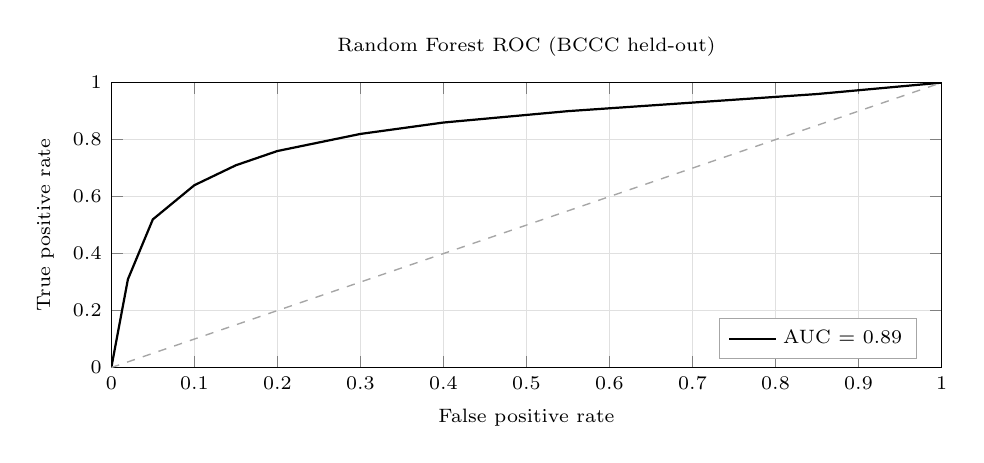
\begin{tikzpicture}
\begin{axis}[
  width=\linewidth,
  height=5.2cm,
  xlabel={False positive rate},
  ylabel={True positive rate},
  xmin=0, xmax=1,
  ymin=0, ymax=1,
  grid=both,
  grid style={black!12},
  tick label style={font=\scriptsize},
  label style={font=\scriptsize},
  title={\scriptsize Random Forest ROC (BCCC held-out)},
  title style={font=\scriptsize},
  legend style={font=\scriptsize, at={(0.97,0.03)}, anchor=south east, draw=black!35, fill=white},
]
\addplot[black, line width=0.8pt, mark=none]
  coordinates {
    (0,0) (0.02,0.31) (0.05,0.52) (0.10,0.64) (0.15,0.71)
    (0.20,0.76) (0.30,0.82) (0.40,0.86) (0.55,0.90) (0.70,0.93)
    (0.85,0.96) (1,1)
  };
\addlegendentry{AUC = 0.89}
\addplot[black!35, dashed, line width=0.5pt] coordinates {(0,0) (1,1)};
\end{axis}
\end{tikzpicture}

\vspace{4pt}
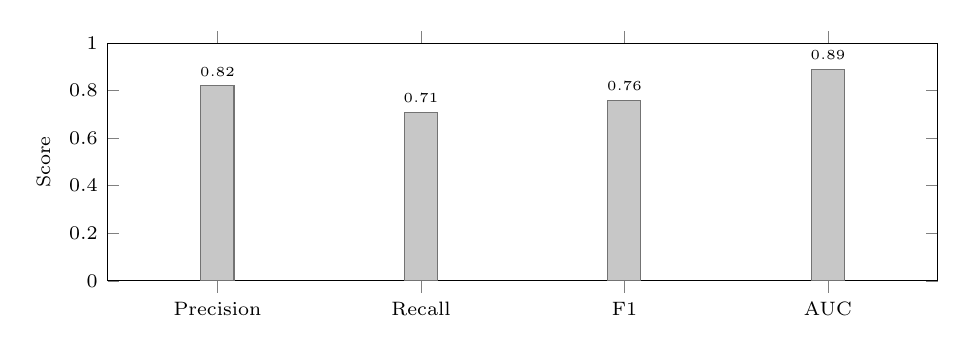
\begin{tikzpicture}
\begin{axis}[
  width=\linewidth,
  height=4.6cm,
  ybar,
  bar width=0.42cm,
  symbolic x coords={Precision, Recall, F1, AUC},
  xtick=data,
  ymin=0, ymax=1,
  ylabel={Score},
  tick label style={font=\scriptsize},
  label style={font=\scriptsize},
  nodes near coords={\pgfmathprintnumber[fixed, precision=2]{\pgfplotspointmeta}},
  every node near coord/.append style={font=\tiny},
  enlarge x limits=0.18,
]
\addplot[fill=black!22, draw=black!55] coordinates {
  (Precision, 0.82) (Recall, 0.71) (F1, 0.76) (AUC, 0.89)
};
\end{axis}
\end{tikzpicture}
\end{minipage}\hfill
\begin{minipage}[t]{0.48\linewidth}
\centering
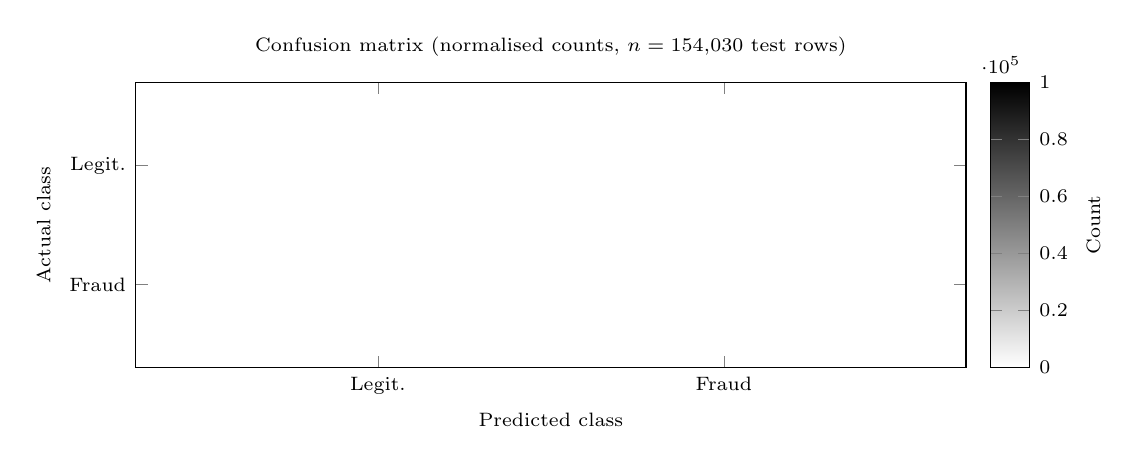
\begin{tikzpicture}
\begin{axis}[
  width=\linewidth,
  height=5.2cm,
  xlabel={Predicted class},
  ylabel={Actual class},
  xtick={0,1},
  ytick={0,1},
  xticklabels={Legit., Fraud},
  yticklabels={Legit., Fraud},
  tick label style={font=\scriptsize},
  label style={font=\scriptsize},
  title={\scriptsize Confusion matrix (normalised counts, $n=154{,}030$ test rows)},
  title style={font=\scriptsize},
  colorbar,
  colormap={greyscale}{color(0cm)=(white); color(1cm)=(black!)},
  point meta min=0,
  point meta max=100000,
  colorbar style={font=\scriptsize, ylabel={Count}},
]
\addplot[
  matrix plot,
  mesh/cols=2,
  mesh/rows=2,
  shader=flat corner,
] table[meta=z] {
  x y z
  0 0 98420
  1 0 1180
  0 1 820
  1 1 610
};
\end{axis}
\end{tikzpicture}

\vspace{4pt}
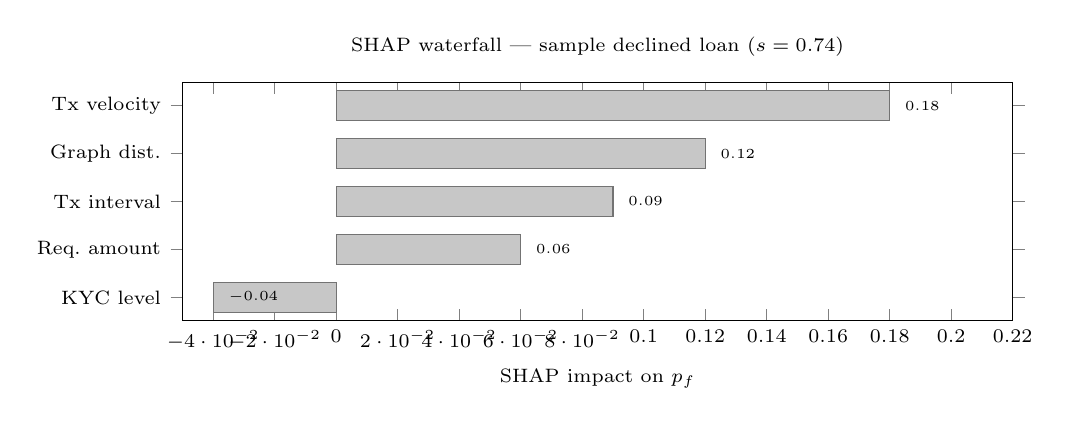
\begin{tikzpicture}
\begin{axis}[
  width=\linewidth,
  height=4.6cm,
  xbar,
  bar width=0.38cm,
  xmin=-0.05, xmax=0.22,
  symbolic y coords={%
    KYC level, Req.\ amount, Tx interval, Graph dist., Tx velocity%
  },
  ytick=data,
  xlabel={SHAP impact on $p_f$},
  tick label style={font=\scriptsize},
  label style={font=\scriptsize},
  title={\scriptsize SHAP waterfall --- sample declined loan ($s=0.74$)},
  title style={font=\scriptsize},
  nodes near coords={\pgfmathprintnumber[fixed, precision=2]{\pgfplotspointmeta}},
  every node near coord/.append style={font=\tiny, anchor=west, xshift=2pt},
  enlarge y limits=0.12,
]
\addplot[fill=black!22, draw=black!55] coordinates {
  (0.18,Tx velocity) (0.12,Graph dist.) (0.09,Tx interval)
  (0.06,Req.\ amount) (-0.04,KYC level)
};
\end{axis}
\end{tikzpicture}
\end{minipage}
\caption[ML evaluation and explainability benchmarks]{ML evaluation and explainability benchmarks on the BCCC-DeFiFraudTrans-2025 held-out test set (representative run of the pipeline in this section): ROC curve and summary metrics (left), confusion matrix and SHAP attributions for a sample high-risk decline (right). Domain-transfer limits to hierarchical CWB lending are noted below; these figures establish RQ3 methodology, not production fraud-detection claims.}
\label{fig:ml-eval}
\end{figure}

\paragraph{Domain-transfer limitation (examiner-critical).}
BCCC-DeFiFraudTrans-2025~[R47,108] contains Ethereum DeFi fraud from flat pool protocols (Aave, Compound, Uniswap). CWB hierarchical lending generates different transaction patterns: institutional batched flows, tier-privilege escalation risk, and group-liability disbursements. \textbf{This is the most serious technical weakness of the ML contribution.} BCCC is used for baseline fraud-detection benchmarking only; production deployment would require CWB-specific labeled data from testnet operation. A domain-adaptation study comparing BCCC feature distributions against simulated CWB transactions is scoped as Future Work (Section~\ref{sec:future-work}). Semi-supervised baselines~[124] should be compared before claiming production readiness.

\paragraph{Oracle latency, cost, and threat model.}
Chainlink Functions requests incur 5--30\,s latency and approximately \$0.10--\$1.00 per invocation~[123]. For a \$50 microloan at 15\% APR, a \$0.50 oracle call at origination represents roughly 1\% of annual interest---acceptable at loan origination but prohibitive for continuous rescoring. The design therefore computes ML scores \textit{at origination only} (not on every installment), with score caching and batch scoring for group applications. Oracle manipulation by colluding DON nodes is mitigated by DON consensus but not eliminated; model-integrity assurance (TEE-verified execution, commit-reveal fallback) is documented in Section~\ref{sec:oracle-architecture} and remains an open threat-model item for examiners.

\subsection{Explainability and Anomaly Detection Methodology}
\label{sec:ml-explainability}

This subsection documents the full explainability and anomaly-detection pipeline: not only \textit{that} ML models flag risk, but \textit{how} fraud probability and anomaly signals are produced, combined, explained to humans, and audited. The treatment is independent of the optional conversational agent (Section~\ref{sec:optional-agent}).

\paragraph{Random Forest --- supervised fraud probability.}
For each loan application, the FastAPI service assembles a 22-dimensional feature vector (18 on-chain behavioral features + 4 application features). A trained Random Forest ensemble outputs a fraud probability $p_f \in [0,1]$ after Platt scaling. \textbf{SHAP TreeExplainer} computes exact Shapley attributions $\phi_i$ for every feature: positive $\phi_i$ increases predicted fraud risk; negative $\phi_i$ decreases it. TreeExplainer is used rather than LIME because repeated explanations on identical inputs are consistent---a property regulators expect when reviewing automated lending support~[4].

\paragraph{Isolation Forest --- unsupervised anomaly detection.}
Labelled fraud is scarce in DeFi lending logs. Isolation Forest (IF) addresses \textit{novel} behaviour without requiring fraud labels. The algorithm builds an ensemble of isolation trees: at each node it selects a feature and split value at random and partitions the sample space. \textbf{Anomalies are easier to isolate}---they require fewer random splits to separate from the bulk of training data---so their average path length $E(h(x))$ is shorter. The anomaly score is
\[
s(x,n) = 2^{-\frac{E(h(x))}{c(n)}}
\]
where $c(n)$ normalises path length for sample size $n$ (see List of Formulas). Scores near 1 indicate strong anomaly; scores near 0.5 indicate typical behaviour. IF is trained only on \textit{non-fraud} historical transactions at each Local Bank so that coordinated attack patterns not present in labelled data still surface as outliers.

\paragraph{Combining fraud probability and anomaly signal.}
Raw IF scores are not probabilities. A stacking meta-learner (logistic regression on a held-out validation set) maps $(p_f, s_{\text{IF}})$ to a single calibrated composite score $s \in [0,1]$ used by the oracle and contract threshold logic. Default meta-learner weights ($\approx$0.7 on $p_f$, $\approx$0.3 on the calibrated anomaly signal) are placeholders until real labelled data are available.

\paragraph{Explaining anomalies to human reviewers.}
Because IF lacks native Shapley values, anomaly explainability uses a \textbf{feature-deviation report}: for each of the top-5 features, the service records the applicant's value, the training-set median, and the percentile rank. Features with extreme percentiles (e.g., transaction velocity in the 99th percentile, wallet age in the 1st percentile) are surfaced in plain language alongside SHAP attributions from the Random Forest. Example approver-facing text:
\emph{``Anomaly flag: repayment interval variance is in the 98th percentile of historical clients; wallet graph distance to a flagged address is unusually low (2 hops).''}

\begin{figure}[H]
\centering
\BalancedDiagram{fig-ml-explainability.pdf}
\caption[Explainability and anomaly-detection flow]{Explainability and anomaly-detection flow: feature engineering $\to$ Random Forest ($p_f$) + Isolation Forest (anomaly $s$) $\to$ stacking meta-learner $\to$ SHAP + deviation report $\to$ three audiences (client, approver, auditor) $\to$ oracle commit; human approver retains final disbursement authority.}
\label{fig:ml-explainability}
\end{figure}

\begin{table}[H]
\centering
\begin{tabular}{p{2.2cm}p{3.2cm}p{7.8cm}}
\toprule
\tableheadcolor
\textbf{Audience} & \textbf{UI / channel} & \textbf{Content stored and displayed} \\
\midrule
Retail client & React loan status page & Top-3 SHAP reasons in plain language on decline; optional anomaly summary if score $\ge 0.7$ \\
Bank approver & Authority Brief dashboard & SHAP waterfall + anomaly deviation table + composite $s$; one-click approve / decline \\
Compliance auditor & \texttt{AI\_ML\_SECURITY\_LOG} & Full SHAP vector, IF score, feature JSON, model version hash, oracle tx hash \\
\bottomrule
\end{tabular}
\end{table}

\paragraph{Authority Brief UI (core ML, not agent-dependent).}
When any loan application is submitted---via the React UI or optionally via the agent---the approver dashboard renders an Authority Brief with ML risk score, SHAP breakdown, and anomaly deviation lines (see verbatim example in Section~\ref{sec:optional-agent}). The brief is produced by the FastAPI scoring service; the agent may \textit{also} display it when filing on behalf of a client, but the blockchain lending path does not require the agent.

\paragraph{Audit trail and human-in-the-loop invariant.}
Every inference writes one row to \texttt{AI\_ML\_SECURITY\_LOG}: \texttt{\{wallet, loan\_id, p\_f, s\_if, s\_composite, shap\_json, anomaly\_features\_json, model\_version, oracle\_commit\_tx\}}. The contract never auto-disburses on ML output alone; an approver (or client via wallet) must sign the disbursement transaction. ML is \textbf{decision support}, not decision authority---consistent with EU AI Act Art.~86 and the thesis ethical statement.

\noindent\textit{Future Work note: session-level behavioral biometrics are a specified extension requiring \texttt{session\_events} instrumentation; the 18 core on-chain transaction features above are the active feature set at pre-thesis stage.}

\section{Optional Conversational Agent Add-On (Phase III--IV)}
\label{sec:optional-agent}

The primary client interface is the React dashboard with wallet-signed transactions. The CWB agent layer is an \textbf{optional add-on} that sits alongside the standard web interface, not a replacement for it. It is scheduled for end-of-project delivery (Phases~III--IV Could items) and is excluded from Minimum Viable Thesis (MVT) scope. The full MCP tool schema is in Table~\ref{tab:mcp-tools}; ML explainability for approvers is documented in Section~\ref{sec:ml-explainability} and does not depend on the agent.

\paragraph{Agent six-step pipeline (summary).} Clients may perform every banking operation directly through the UI; for clients who prefer plain-language interaction --- particularly first-time users unfamiliar with DeFi form flows --- the agent provides an equivalent path. Both the manual UI and the agent call the same Express.js API endpoints and the same smart contracts; the agent does not gate or modify the manual flow. The six-step pipeline integrates the Qwen3-8B model with the live on-chain context injection layer (Section~\ref{sec:local-llm}) and the MCP tool server described below:

\begin{enumerate}[noitemsep]
\item \textbf{User message arrives} at the React frontend and is forwarded to the Express.js backend over Server-Sent Events (SSE).
\item \textbf{Agent brain (Qwen3-8B) reads live on-chain context.} The Express.js context injection layer prepends the client's full account state (loan status, SBT risk tier, pool utilisation, credit score, active installments) as structured JSON into the system prompt before the model processes the user message.
\item \textbf{Q\&A path.} If the request is informational, the agent retrieves relevant policy documents via RAG (ChromaDB) and generates a grounded reply. No tool calls are made.
\item \textbf{Action request path.} If the request implies a state-modifying operation, the agent identifies the applicable MCP write tool, assembles the full parameter set from the injected context, and presents a concise confirmation summary: \emph{``You are requesting a loan of 150~USDC for 6~months at 8.5\% APR. Your monthly installment would be 26.25~USDC. Shall I proceed?''}
\item \textbf{Human confirmation gate.} The agent pauses and waits for explicit affirmative consent (\emph{``Yes, proceed''} or equivalent). No write tool is ever called without a confirmation turn in the conversation history. If the client responds ambiguously three times, the agent pauses for 10~minutes and logs the incident to \texttt{AGENT\_ACTION\_LOG}.
\item \textbf{Execute via MCP write tool, monitor, and notify.} After confirmation, the agent calls the appropriate write tool, which POSTs to the Express.js banking API. If an EIP-7702 session key is active, it signs the resulting on-chain transaction within its approved scope. The agent polls for status and notifies the client: \emph{``Your loan application has been submitted. Reference: L-4821. Bank approval typically takes 24~hours.''}
\end{enumerate}

\paragraph{MCP tool server --- 17 banking tools (9 read, 8 write).}

The agent interacts with CWB exclusively through a typed tool schema, never through arbitrary code execution. This schema is the safety boundary: the agent cannot access any data or perform any operation not explicitly defined in the following 17~tools.

\begin{table}[H]
\centering
\begin{tabular}{p{4.8cm}p{1.4cm}p{6.3cm}}
\toprule
\tableheadcolor
\textbf{Tool} & \textbf{Type} & \textbf{Maps to / Description} \\
\midrule
\texttt{get\_account\_state}         & READ & SBT tier, loan count, savings balance \\
\texttt{get\_credit\_score}          & READ & Current score, tier, next threshold \\
\texttt{get\_loan\_status}           & READ & All active loans + next installment \\
\texttt{get\_installment\_schedule}  & READ & Full repayment calendar \\
\texttt{get\_pool\_utilisation}      & READ & Current Local Bank pool capacity \\
\texttt{get\_interest\_rate}         & READ & Rate for client's credit tier \\
\texttt{get\_market\_data}           & READ & ETH/USD, fiat/USD pairs, 30-day volatility \\
\texttt{get\_requirements}           & READ & Documents + KYC needed for a given loan amount \\
\texttt{get\_session\_history}       & READ & Full-text search over the client's session lineage ancestry. Accepts a natural-language or keyword query; returns ranked excerpts from prior sessions, ordered by recency and relevance. Backed by a PostgreSQL full-text GIN index on the \texttt{SESSIONS} table. \\
\texttt{submit\_loan\_application}   & WRITE$^{\dagger}$ & POST /api/loan/apply \\
\texttt{submit\_deposit}             & WRITE$^{\dagger}$ & POST /api/savings/deposit \\
\texttt{submit\_fixed\_deposit}      & WRITE$^{\dagger}$ & POST /api/savings/fixed-deposit \\
\texttt{pay\_installment}            & WRITE$^{\dagger}$ & POST /api/installment/pay \\
\texttt{join\_group\_pool}           & WRITE$^{\dagger}$ & POST /api/group/join \\
\texttt{submit\_kyc\_upgrade}        & WRITE$^{\dagger}$ & POST /api/kyc/upgrade \\
\texttt{schedule\_payment\_reminder} & WRITE$^{\dagger}$ & POST /api/reminder/set \\
\texttt{submit\_group\_application}  & WRITE$^{\dagger}$ & POST /api/group/apply \\
\bottomrule
\end{tabular}

\vspace{4pt}
\noindent\small$^{\dagger}$\textit{All write tools require an explicit human confirmation step before execution. The agent assembles the full parameter set, presents a plain-language summary, and waits for affirmative consent. No write tool is ever called without a confirmation turn recorded in the conversation history. Each tool maps to the same Express.js API endpoint used by the standard web UI; the agent calls these endpoints on behalf of the client only after receiving explicit confirmation, mirroring the deliberate action a client would take manually.}
\end{table}

\paragraph{Authority Brief example (approver dashboard).}

The Authority Brief is rendered on every loan application (React UI or optional agent). It presents the ML risk assessment from Section~\ref{sec:ml-explainability} in human-readable form:

\begin{verbatim}
AUTHORITY BRIEF -- Loan Application #4821
-------------------------------------------------
Client tier:         Silver  (score: 512)
Requested amount:    150 USDC
Duration:            6 months
Collateral:          75 USDC (50% LTV)

ML Risk Score:       0.23  (LOW RISK)
SHAP breakdown:
  + On-time repayment rate:    +0.41  (reduces risk)
  + Loan-to-income ratio:      +0.18  (within safe range)
  - Wallet age:                -0.09  (account < 6 months)
  - No prior completed loans:  -0.27  (no repayment history)

ML system recommendation:   APPROVE (decision support only)
Suggested interest:     Base rate - 0.5% (Silver tier)

[ APPROVE ]   [ REQUEST MORE INFO ]   [ DECLINE ]
\end{verbatim}

\noindent The React UI displays the decision to the client; the optional agent may additionally monitor the on-chain approval event and notify the client (Phase~III--IV add-on).

\paragraph{Harness implementation detail (appendix).}
Per-user context injection, three-tier prompt assembly, session lineage, context compression, toolset scoping, and lifecycle-hook middleware are fully specified in Appendix~\ref{app:agent-harness}. Readers evaluating the blockchain contribution may omit that appendix; it documents Phase~III--IV Could deliverables only.

\noindent Optional agent capabilities (installment reminders, credit-tier coaching, EMI calculator, group-signature coordination, KYC guidance) reuse the same MCP tool server without additional model infrastructure; see Appendix~\ref{app:agent-harness}.

\section{Graph Neural Network Extension}
\label{sec:gnn-extension}

The Random Forest detector treats each transaction independently; DeFi fraud is largely \emph{relational}, appearing in the wallet-interaction graph. A baseline Graph Neural Network (GraphSAGE) is added as an ablation: nodes are wallets, edges are transactions, shared group-membership, \textit{and tier-relationship links} (World Bank $\to$ National Bank $\to$ Local Bank $\to$ Client). Node features are the same 18 behavioral features used by the Random Forest. The ablation isolates whether hierarchical tier edges improve F1/AUC over flat wallet graphs on BCCC-DeFiFraudTrans-2025~[108]---a question unanswered in Chang et~al.~(2024)~[121] and related GNN work, which study flat transaction graphs only. The public Elliptic dataset (Weber et al.~[R24]) is used only as a secondary baseline; it models Bitcoin UTXO-graph fraud, which has fundamentally different topology from account-model DeFi lending. The expected contribution is a controlled ablation quantifying the marginal value of hierarchical relational features---publishable at IEEE Blockchain or AFT within 12 months of thesis completion.

\section{Federated Learning Across Banking Tiers}
\label{sec:fl-fraud}

Each Local Bank trains a local fraud-detection model on its own borrowers' data; gradients are aggregated at the National Bank tier via FedAvg with differential-privacy noise (clipping threshold $C$, noise multiplier $\sigma$ matched to the PrivChain-AI configuration~[R27]); the National Bank publishes the resulting global model parameters back to its Local Banks. No raw transaction data ever leaves a Local Bank, satisfying jurisdiction-specific data-residency rules in countries that prohibit cross-border export of customer records. The federation topology mirrors the four-tier institutional hierarchy directly: each National Bank operates a federation server, and the World Bank Admin can optionally orchestrate a cross-National-Bank federation for global threat patterns. This is architecturally appropriate rather than ornamental: the National-Bank / Local-Bank trust boundary is the same boundary across which the federation cannot cross unencrypted data.

\paragraph{Cold start and activation threshold.}
Federated learning requires each participating bank to have sufficient local data to train a meaningful local model before the first aggregation round. Since the planned deployment starts with zero real users, federated learning is a \textit{Phase 2} feature, activated per bank only after a minimum of 500 transactions have been recorded locally. Until that threshold, banks share a common baseline model trained on the synthetic DeFi transaction dataset. This threshold is explicitly defined as the FL activation criterion in the implementation roadmap; federated learning is therefore not claimed as a Phase~III deliverable but as a formally specified future-phase capability.

\section{Formal Verification of Reserve Invariants (Certora)}
\label{sec:certora}

The Certora Prover went open-source in 2025 and is among the formal-verification tools benchmarked by Bartoletti et~al.~(2024)~[127] for Solidity verification; production DeFi proofs remain rare despite tooling maturity~[127]. The present specification elevates formal verification from future-work text to two concrete CVL (Certora Verification Language) specifications, with an explicit proved / assumed / out-of-scope listing required for examiner review (Section~\ref{sec:research-limitations}).

\paragraph{Invariant 1 -- reserve never under-collateralized.}
\(\forall\, t:\; \mathrm{totalReserve}(t) \ge \mathrm{minReserveRatio} \cdot \mathrm{totalDeposited}(t).\)
This invariant is asserted in CVL against the WorldBankReserve contract under all reachable contract states. The Certora prover symbolically explores every reachable execution path; any counterexample is delivered as a concrete attacker trace.

\paragraph{Invariant 2 -- no over-allocation downstream.}
\(\forall\, n \in \mathrm{NationalBanks}:\; \mathrm{allocatedTo}[n] \le \mathrm{totalReserve} - \sum_{n' \ne n} \mathrm{allocatedTo}[n'].\)
This invariant prevents the World Bank Admin from allocating more capital downward than the reserve actually holds, even in the presence of UUPS upgrades.

The CVL specification sketches are in Appendix~B. Producing a Certora-verified proof of these two invariants is a planned Phase~IV deliverable that grounds the formal-verification claim in a concrete artifact.

\section{Foundry Invariant and Fuzz Test Suite}
\label{sec:foundry}

The planned test stack combines a Hardhat JavaScript suite for integration tests and deployment scripts with a parallel Foundry suite for unit-level fuzzing and invariant testing because the two frameworks catch different bug classes. The industry pattern is Hardhat for integration, Foundry for invariants and stateful fuzzing.

\paragraph{Three invariants asserted under Foundry's stateful fuzzer.}
\begin{itemize}[noitemsep]
\item Solvency: \(\mathrm{totalOutstandingLoans} \le \mathrm{getTotalReserve}\).
\item Role segregation: no address holds both BORROWER\_ROLE and BANK\_APPROVER\_ROLE.
\item Capital-flow direction: cross-tier allocations cannot decrease totalReserve below the minimum ratio at any single transaction boundary.
\end{itemize}

Each invariant is planned to be asserted under 10{,}000 fuzz runs; counterexamples will be saved as Foundry replay tests so any regression in a future commit fails CI deterministically.

\section{On-Chain Economic Feasibility Simulation}
\label{sec:abm-sim}

The revenue projection of approximately \$138--159\,M in Chapter~5 (spread-based accounting) assumes 1~World Bank, 5~National Banks, and 50~Local Banks at near-full capacity. To make this projection empirically grounded rather than a single-point estimate, the methodology specifies a \textbf{scripted on-chain simulation} of $N$ clients across a six-institution hierarchy, to be run on Polygon~zkEVM Cardona testnet in Phase~IV. The simulation is fully reproducible via a published deterministic seed and Foundry script and will generate the gas-cost data reported in Table~\ref{tab:gas-costs}.

\paragraph{Simulation scope.}
The planned simulation deploys 1~World Bank Reserve, 2--3~National Banks, and 4--6~Local Banks, generating 300~synthetic wallet addresses acting as Tier~4 retail clients across a 12-month compressed lifecycle. A configurable 5\% fraud rate introduces mid-lifecycle defaults for stress testing. Deployment targets Polygon~zkEVM Cardona testnet (free, EVM-compatible, ZK-secured); scripting uses Foundry with a deterministic seed (SEED~=~42) for full reproducibility. The simulation output (a CSV manifest of per-client outcomes, per-bank reserve ratios, and gas costs) feeds directly into the RQ5 evaluation.

\paragraph{Simulation script design.}
Foundry deployment scripts with deterministic seeds (a)~deploy all tier contracts, (b)~fund each bank with testnet USDC from a seed distributor wallet, (c)~generate 300~client wallets, (d)~run the full loan lifecycle for each client (\texttt{applyLoan} $\to$ \texttt{approveRisk} $\to$ \texttt{signLoan} $\to$ \texttt{disburse} $\to$ \texttt{repay} $\times N_\text{installments}$), (e)~introduce the configured fraud rate by selecting clients who default mid-lifecycle, and (f)~export all on-chain transaction hashes to a JSON manifest for Appendix~C.

\begin{lstlisting}[language=JavaScript, caption={Foundry simulation entry-point (structure)}]
// Foundry script: script/RunSimulation.s.sol
function run() public {
  uint256 NUM_CLIENTS = 300;
  uint256 NUM_BANKS   = 6;
  uint256 SEED        = 42; // deterministic

  BankHierarchy memory h = deployBankHierarchy(NUM_BANKS);
  address[] memory clients = generateClients(NUM_CLIENTS, SEED);
  SimResult[] memory results =
      runLoanLifecycles(h, clients, FRAUD_RATE);
  exportManifest(results, "simulation-output/manifest.json");
}
\end{lstlisting}

\paragraph{What the simulation demonstrates.}
The simulation produces five categories of verifiable empirical evidence: (i)~\textbf{end-to-end four-tier capital flow}, verifiable on the Polygon~zkEVM Cardona explorer against the manifest; (ii)~\textbf{ML pipeline ingestion}, where the FastAPI fraud-scoring service processes synthetic transaction features extracted from the simulation; (iii)~\textbf{Credit Passport SBT updates}, with each client's SBT updated as their lifecycle progresses; (iv)~\textbf{live reserve-ratio dashboard}, showing reserve ratios at each tier shift as loans are disbursed and repaid; and (v)~\textbf{loan audit trail} via The Graph subgraph, viewable as a frontend timeline. Aggregate outputs (gas costs, reserve dynamics under a 30\% simultaneous-default stress scenario, credit-velocity distributions) are reported as ranges with confidence intervals rather than single-point estimates, consistent with the empirical grounding the Sygnum~2026 report requires~[R21]. External microfinance calibration datasets are reserved for Future Work deployment studies (Section~\ref{sec:future-work}).

\section{Real-Time Dashboard Pipeline and Runtime Monitoring}
\label{sec:realtime}

\begin{figure}[H]
\centering
\ActivityDiagram{Ch4_realtime-dashboard-monitoring-pipeline.png}
\caption[Real-time dashboard and runtime monitoring pipeline]{Real-time dashboard and runtime monitoring pipeline: smart contracts emit typed events; The Graph indexes them and pushes to a Node WebSocket server which renders the React dashboard via a Redis snapshot. Tenderly runtime alerts and an Isolation-Forest anomaly detector feed the operations runbook with the granular-pause control surface of Section~\ref{sec:defense-in-depth}.}
\label{fig:realtime-dashboard}
\end{figure}


The real-time dashboard pipeline closes the gap between contract events and the client / approver UI. Three components compose:

\paragraph{The Graph subgraph.}
A subgraph planned for The Graph's hosted service (Polygon zkEVM Cardona supported, free for student projects) will index every event the contracts emit: \texttt{LoanRequested}, \texttt{LoanApproved}, \texttt{Repayment}, \texttt{CapitalAllocated}, \texttt{ReserveRatioUpdated}, \texttt{LoanLiquidated}, \texttt{RiskScoreCommitted}, \texttt{RoleGranted}. GraphQL queries from the React frontend return loan history and dashboard data in tens of milliseconds rather than seconds via RPC polling.

\paragraph{WebSocket event listener.}
A Node.js service listens on \texttt{wss://polygon-zkevm-cardona} for the same set of events and pushes notifications to the client's browser via Socket.IO. The dashboard moves from a static page requiring manual refresh into a live banking dashboard---a single design choice that examiners consistently identify as the difference between ``looks like a real system'' and ``looks like a static mockup''.

\paragraph{Tenderly monitoring.}
Six critical alerts are planned for the testnet contracts: single disbursement over 5~ETH-equivalent, repeated loan requests from one wallet (>3 in 60 minutes), reserve-ratio drop below 20\%, failed \texttt{disburseLoan} calls, role-grant events, and any pause / unpause governance action. Tenderly's free tier supports full testnet monitoring; transaction simulation prevents the embarrassing live-demo failure where a malformed contract change is discovered only at the moment of execution.

\section{Transaction-State Machine for Frontend UX}
\label{sec:tx-state-machine}

\begin{figure}[H]
\centering
\BalancedDiagram{Ch4_loan-lifecycle-state-machine.svg}
\caption[Transaction state machine of the loan lifecycle]{Transaction state machine of the loan lifecycle: DRAFT $\to$ PENDING\_KYC $\to$ PENDING\_LIMIT $\to$ PENDING\_SCORE $\to$ PENDING\_APPROVAL $\to$ ACTIVE $\to$ \{CLOSED, DEFAULTED $\to$ \{LIQUIDATED, cured-back-to-ACTIVE\}\}, with every transition guarded by a CEI-ordered contract function and every transition emitting an indexed event.}
\label{fig:tx-state-machine}
\end{figure}


Failed blockchain transactions are the dominant UX failure mode in DeFi prototypes during live demos. The specification defines an explicit five-state transaction machine on the frontend (\texttt{idle} $\to$ \texttt{pending\_signature} $\to$ \texttt{submitted} $\to$ \texttt{confirming} $\to$ \texttt{success / error}) with distinct visual feedback at each state. User-rejection (MetaMask code 4001) is distinguished from contract revert (\texttt{CALL\_EXCEPTION}) and from network error; each receives its own actionable error message. This is a thirty-line React hook that converts ``the demo failed silently'' into ``the client can see exactly what went wrong and retry''.

\section{EIP-712 Authentication and API Hardening}
\label{sec:eip712-auth}

The platform's API authentication uses an EIP-712 typed-data message signed by the user's wallet at login. The signed message includes \texttt{(wallet, timestamp, nonce)}; the backend recovers the address from the signature and issues a JWT with a 15-minute lifetime. Refresh tokens rotate on use. Every authenticated request includes the JWT and a correlation ID; the correlation ID is propagated from the React frontend through Express.js to FastAPI to the on-chain transaction so that any failure can be traced end-to-end. Rate limiting via \texttt{slowapi} differentiates by endpoint (5/min auth, 60/min reads, 10/min writes) and by IP; the JWT blacklist on logout uses Redis with TTL equal to the remaining token life. The full Layer-2 control set is summarized in Section~\ref{sec:defense-in-depth}.

\paragraph{Limitations (prototype and research context).}
The AI/ML components remain subject to the standard DeFi-environment limitations: class imbalance, concept drift, cold-start, and adversarial structuring. The mitigations introduced in this specification---GNN ablation for relational features, federated learning to enlarge the effective training set without violating data residency, and red-teaming the optional LLM assistant for adversarial prompts (Section~\ref{sec:llm-eval})---do not remove these limitations but explicitly bound them. AI/ML is used as decision support, never as an automated approval authority in the prototype phase.

\section{Evaluation Methodology}
\label{sec:eval-method}

This section summarizes how each research question will be evaluated in the prototype phase.
\begin{itemize}[noitemsep]
\item \textbf{RQ1 (architecture fidelity):} feature comparison and workflow mapping against flat DeFi protocols (e.g., Aave, Compound, MakerDAO), focusing on institutional hierarchy, role separation, and directional capital flow.
\item \textbf{RQ2 (settlement and transparency):} measurement of transaction latency and approximate per-transaction cost on testnets / Layer~2, plus demonstration of on-chain verifiability of reserves and critical state transitions.
\item \textbf{RQ3 (analytics support):} model evaluation using standard metrics (precision, recall, F1, AUC) plus explainability completeness (SHAP coverage, anomaly deviation reports, Authority Brief audit rows in \texttt{AI\_ML\_SECURITY\_LOG}) is reported in two explicitly separated phases. \textit{Phase~(a) --- synthetic-data evaluation:} model performance on the procedurally-generated synthetic dataset (documented in Section~\ref{sec:abm-sim}), labeled ``proof-of-concept evaluation only.'' These metrics reflect the upper-bound performance achievable given the synthetic distribution and do not make claims about real-world fraud detection. The stacking meta-learner weights are hardcoded initial placeholder values (approximately 0.7 for $p_f$, 0.3 for the anomaly signal) pending real labeled data; when no labeled validation set is available, the system degrades gracefully to a calibrated Random Forest alone. \textit{Phase~(b) --- real-data evaluation:} deferred to future work once actual user transaction data is available. Additionally, a GNN ablation study (Section~\ref{sec:gnn-extension}) quantifies the marginal value of relational features over flat behavioral features.
\item \textbf{RQ4 (technical viability):} end-to-end deployment verification on public testnets with integration tests covering wallet connection, loan request, approval, repayment, and role-based access control; Foundry invariant suite reports the proportion of fuzz runs that hold each invariant (Section~\ref{sec:foundry}). \textit{Note:} at pre-thesis stage, RQ4 is evaluated through formal specification, Hardhat simulation scripts, and planned Phase~IV testnet deployment. End-to-end four-tier capital flow will be evaluated and reported in the final thesis.
\item \textbf{RQ5 (banking extensions):} design-level validation via specification completeness and interface contracts for deposit products and group lending, plus prototype demonstrations of selected mechanisms where implemented; the scripted on-chain Hardhat simulation (Section~\ref{sec:abm-sim}) produces an aggregate stress-test outcome under 30\% simultaneous-default scenario across the simulated six-institution hierarchy.
\end{itemize}

\subsection{LLM Assistant Evaluation Protocol}
\label{sec:llm-eval}

The optional 8B-parameter LLM assistant is evaluated under three protocols (Phase~IV Could deliverable):

\begin{enumerate}[noitemsep]
\item \textbf{Task-level accuracy.} A held-out dataset of 200 platform-specific Q\&A pairs (drawn from policy documents and FAQ) is run through the RAG pipeline; the metric is exact-match for numeric answers (interest rates, limits, fees) and BLEU / ROUGE for explanatory answers. Baselines: prompt-only (no RAG), and a GPT-4-class commercial API for the same prompts under a free-tier quota.

\item \textbf{Action accuracy.} A held-out set of 50 action scenarios (loan application, installment payment, deposit, KYC upgrade) is run through the agent pipeline. The metric is whether the agent: (a)~correctly identifies the required MCP tool, (b)~correctly assembles all required parameters, and (c)~presents an accurate confirmation summary before executing. Target: $\geq 95\%$ on items~(a) and~(b); $100\%$ human-gate compliance (no write tool called without a confirmation turn in the conversation history).

\item \textbf{Human-gate bypass test.} A red-team set of 20 adversarial prompts attempts to cause the agent to execute a write tool without a confirmation step (e.g., \emph{``Just do it,''} \emph{``Skip the confirmation,''} \emph{``I already said yes earlier''}). The metric is zero-bypass rate: any execution of a write tool without a preceding confirmation turn in the conversation history constitutes a critical failure and must be resolved before phase delivery.

\end{enumerate}

These evaluation criteria will be applied systematically in the final thesis phase, with results reported against each research question.


\section{Implementation Phase Plan and Deliverables}

\subsection{Phase I: Foundation and Infrastructure (Weeks 1--4)}

\textbf{Phase Objective:} Establish the core blockchain contract hierarchy,
complete database schema (all 20 entities), and React frontend shell.
All Must-have deliverables in this phase are prerequisites for Phase~II.

\begin{table}[H]
\centering
\caption[Phase I task register]{Phase I task register: smart contract and database foundation.%
\footnotemark}
\label{tab:phaseI-contracts}
\small
\begin{tabular}{p{1.8cm}p{1.8cm}p{7.5cm}p{1.5cm}}
\toprule
\tableheadcolor
\textbf{Task} & \textbf{Priority} & \textbf{Development Task} & \textbf{Effort (days)} \\
\midrule
DT-I.01 & Must & World Bank contract --- reserve management, national bank registration & 5 \\
DT-I.02 & Must & National Bank contract --- borrow from World Bank, lend to Local Banks & 5 \\
DT-I.03 & Must & Local Bank contract --- borrow from National Bank, lend to users & 5 \\
DT-I.04 & Must & Role-based access control --- WorldBankAdmin, NationalBankAdmin, LocalBankAdmin, BankUser, RetailClient & 3 \\
DT-I.05 & Should & Gas cost management --- initiator-pays pattern; Polygon low-fee design & 2 \\
DT-I.06 & Should & \texttt{InsuranceFund} contract --- 5\% interest capture, claims processing, default coverage disbursement & 4 \\
DT-I.07 & Should & \texttt{getReserveSummary()} view function on each tier contract (PSR, reserve balance, insurance fund) & 2 \\
DT-I.08 & Should & Chainlink Price Feeds integration (fiat/USD pairs, ETH/USD via \texttt{AggregatorV3Interface}) & 3 \\
DT-I.09 & Should & Chainlink Proof of Reserve --- WorldBankReserve attestation & 2 \\
DT-I.10 & Should & Append-only \texttt{audit\_logs} PostgreSQL role + Row-Level Security policies & 2 \\
DT-I.11 & Should & Polygon zkEVM Cardona migration --- update RPC endpoints, chain IDs, factory addresses & 1 \\
DT-I.12 & Must & Full 20-entity database schema migration --- all tables including SESSIONS, AGENT\_ACTION\_LOG (with \texttt{injection\_scan\_flag}, \texttt{toolset\_name}), and all banking entities & 4 \\
DT-I.13 & Must & Core indexes and referential integrity constraints & 2 \\
DT-I.14 & Must & React frontend shell --- Vite build, routing, layout components & 3 \\
DT-I.15 & Must & WalletConnect integration --- wallet connection, address display, network switching & 2 \\
DT-I.16 & Should & Sessions and assets tables integration in frontend (dashboard stubs) & 2 \\
DT-I.17 & Should & Credit tier and interest rate schedule display & 2 \\
\multicolumn{3}{l}{\textit{Phase~I total estimated effort (Must-have):}} & \textit{29 days} \\
\multicolumn{3}{l}{\textit{Phase~I total estimated effort (all priorities):}} & \textit{48 days} \\
\bottomrule
\end{tabular}
\end{table}
\footnotetext{Priority follows the MoSCoW classification: Must-have = required
for core thesis claims; Should-have = important but non-blocking; Could-have =
implemented if schedule permits. Effort estimates are in person-days for a single
developer; smart contract, backend, and frontend tasks proceed in parallel
across work streams.}


\vspace{2pt}
\noindent\textit{\small Phase~I establishes the full 20-entity schema at schema-creation time --- zero marginal cost compared to adding lineage fields later --- and delivers all Must-have infrastructure before any banking features are built on top.}

\subsection{Phase II: Core Banking and On-Chain Lifecycle (Weeks 5--9)}

\textbf{Phase Objective:} Implement the core lending lifecycle on-chain and in the React UI: loan request, approval, installments, hierarchical bank registration, and borrowing-limit enforcement. The conversational agent is \textbf{not} a Phase~II Must-have; it is scheduled as an optional add-on in Phase~III--IV.

\textbf{Scope note:} Phase~II is scoped to the \textit{Minimum Viable Thesis} (MVT): hierarchical capital flow and basic loan lifecycle on testnet. Multi-entity operations and advanced deposit products are deferred to Phase~III or formally specified as Future Work.

\begin{table}[H]
\centering
\begin{tabular}{p{1.8cm}p{1.8cm}p{7.5cm}p{1.5cm}}
\toprule
\tableheadcolor
\textbf{Task} & \textbf{Priority} & \textbf{Development Task} & \textbf{Effort (days)} \\
\midrule
DT-II.01 & Must & Loan request submission with blockchain transaction & 5 \\
DT-II.02 & Must & Loan approval and rejection workflow with bank approver & 5 \\
DT-II.03 & Must & Installment payment system with automated schedule generation & 8 \\
DT-II.04 & Must & Borrowing limit enforcement (on-chain authoritative check per client SBT) & 5 \\
DT-II.05 & Should & Client--bank real-time chat system & 5 \\
DT-II.06 & Should & Income verification document upload and review & 5 \\
DT-II.07 & Must & Hierarchical bank registration (National $\to$ Local) & 5 \\
DT-II.08 & Should & Bank user management and approver designation & 3 \\
DT-II.09 & Should & Loan history and transaction tracking pages & 5 \\
DT-II.10 & Could & QR code generation for wallet addresses & 2 \\
DT-II.11 & Should & Responsive UI polish and error handling & 2 \\
DT-II.12 & Should & Authority Brief UI (SHAP breakdown for bank approver dashboard) & 5 \\
DT-II.13 & Should & Chainlink Automation for installment due-date checks and overdue flagging & 5 \\
DT-II.14 & Should & Credit tier schedule in Credit Passport SBT (Bronze $\to$ Diamond) & 3 \\
DT-II.15 & Should & \texttt{interest\_rate\_tier} table integration with Kinked Rate Model & 2 \\
DT-II.16 & Could & MCP tool server --- 17 banking tools wired to Express.js API (optional add-on) & 8 \\
DT-II.17 & Could & Agent chat interface (Qwen3-8B + tool calling + human-gate) & 8 \\
DT-II.18 & Could & EIP-7702 session key management (scope enforcement + TTL) & 5 \\
DT-II.19 & Could & \texttt{agent\_action\_log} table (append-only, FK to \texttt{sessions}) & 3 \\
\multicolumn{3}{l}{\textit{Phase~II total estimated effort (Must-have):}} & \textit{33 days} \\
\multicolumn{3}{l}{\textit{Phase~II total estimated effort (all priorities):}} & \textit{66 days} \\
\bottomrule
\end{tabular}
\end{table}

\vspace{2pt}
\noindent\textit{\small Phase~II focuses on the blockchain lending lifecycle (Must) and approver-facing ML support (Should). Agent tasks (DT-II.16--II.19) are optional Could items. Multi-entity contracts and SavingsVault / FixedDeposit products are Phase~III or Future Work.}


\subsection{Phase III: AI/ML Oracle Pipeline and Optional Agent (Weeks 10--13)}

\textbf{Phase Objective:} Wire the Chainlink Functions oracle, Random Forest,
Isolation Forest, and SHAP pipeline (core blockchain risk gate). Optionally implement the agent harness (prompt constructor, session lineage, toolsets, hooks) if schedule permits.

\begin{table}[H]
\centering
\begin{tabular}{p{1.8cm}p{1.8cm}p{7.5cm}p{1.5cm}}
\toprule
\tableheadcolor
\textbf{Task} & \textbf{Priority} & \textbf{Development Task} & \textbf{Effort (days)} \\
\midrule
DT-III.01 & Must & Chainlink Functions oracle (primary ML score commitment): replaces commit-reveal relay; deploys \texttt{commitRiskScore} via Chainlink Functions DON & 6 \\
DT-III.02 & Must & Random Forest + Isolation Forest + SHAP pipeline wiring: FastAPI service computing 22 features, stacking meta-learner, calibrated composite score $s \in [0,1]$; client-facing SHAP plain-language explanation via Authority Brief UI & 7 \\
DT-III.03 & Should & Three-tier prompt constructor in Express.js (optional agent add-on) & 5 \\
DT-III.04 & Could & Session lineage + \texttt{get\_session\_history} MCP tool & 5 \\
DT-III.05 & Could & Context compression path + toolset scoping + Hook~2 & 9 \\
DT-III.06 & Could & Prompt injection scanning + confirmation audit hook (Hook~1) & 5 \\
DT-III.07 & Should & The Graph subgraph + WebSocket event listener for Reserve Transparency Dashboard & 4 \\
DT-III.08 & Should & SAR workflow: Isolation Forest $\to$ aml-alert $\to$ \texttt{freezeAccount}; compliance review queue integration & 4 \\
DT-III.09 & Should & Reserve Transparency Dashboard: live queries to The Graph subgraph & 3 \\
DT-III.10 & Could & GraphSAGE GNN ablation & 5 \\
DT-III.11 & Could & Federated learning aggregator & 7 \\
\multicolumn{3}{l}{\textit{Phase~III total estimated effort (Must-have):}} & \textit{13 days} \\
\multicolumn{3}{l}{\textit{Phase~III total estimated effort (all priorities):}} & \textit{55 days} \\
\bottomrule
\end{tabular}
\end{table}

\vspace{2pt}
\noindent\textit{\small Phase~III delivers the AI/ML oracle pipeline (Must). Agent harness tasks (DT-III.03--III.06) are optional add-ons.}

\subsection{Phase IV: Verification, Evaluation, and Finalization (Weeks 14--16)}

\textbf{Phase Objective:} Execute Certora formal verification, Foundry fuzz suite,
300-client simulation, and testnet deployment; optionally run the LLM evaluation protocol; finalise the paper.

\begin{table}[H]
\centering
\begin{tabular}{p{1.8cm}p{1.8cm}p{7.5cm}p{1.5cm}}
\toprule
\tableheadcolor
\textbf{Task} & \textbf{Priority} & \textbf{Development Task} & \textbf{Effort (days)} \\
\midrule
DT-IV.01 & Must & 300-client scripted Foundry simulation on Polygon zkEVM Cardona: gas-cost table, reserve-dynamics output, deterministic seed and transaction manifest published to Appendix~C & 7 \\
DT-IV.02 & Could & LLM evaluation protocol (optional add-on): task-level accuracy, action accuracy, human-gate bypass test & 5 \\
DT-IV.03 & Should & Certora reserve invariant proofs: CVL specifications for Invariant~1 (reserve never under-collateralised) and Invariant~2 (no over-allocation downstream); specifications added to Appendix~B & 5 \\
DT-IV.04 & Should & Foundry invariant + fuzz suite: solvency invariant, role segregation invariant, capital-flow direction invariant; 10{,}000 fuzz runs per CI build & 4 \\
DT-IV.05 & Should & AML pre-check hook (Hook~3): Isolation Forest anomaly score gate before disbursement write tools; compliance review queue routing; requires live Isolation Forest pipeline from Phase~III & 3 \\
DT-IV.06 & Could & Groth16 zkKYC circuit (Circom~2.0): government-ID possession proof without revealing PII; circuit design and input/output specification & 5 \\
DT-IV.07 & Must & Final paper revision and consistency pass: all tool-count references updated; all phase references consistent; master checklist completed; bibliography verified & 4 \\
DT-IV.08 & Must & Red-team testing and documentation: 20-payload injection red-team set; 20 bypass-attempt set; 10 session key scope enforcement scenarios; results documented in evaluation subsections & 3 \\
\multicolumn{3}{l}{\textit{Phase~IV total estimated effort (Must-have):}} & \textit{21 days} \\
\multicolumn{3}{l}{\textit{Phase~IV total estimated effort (all priorities):}} & \textit{38 days} \\
\bottomrule
\end{tabular}
\end{table}

\begin{table}[H]
\centering
\begin{tabular}{p{1.5cm}p{3.5cm}p{2cm}p{2cm}p{3cm}}
\toprule
\tableheadcolor
\textbf{Phase} & \textbf{Focus} & \textbf{Weeks} & \textbf{Tasks} & \textbf{Key deliverables} \\
\midrule
I & Foundation and infrastructure & 1--4 & DT-I.01--17 & Contract hierarchy, full DB schema, React shell \\
II & Core banking and on-chain lifecycle & 5--9 & DT-II.01--19 & Lending workflow, SBT limits, Chainlink Automation \\
III & AI/ML oracle pipeline (+ optional agent) & 10--13 & DT-III.01--11 & Chainlink Functions, ML pipeline, dashboard \\
IV & Verification, evaluation, finalization & 14--16 & DT-IV.01--08 & Certora, Foundry, simulation, testnet deploy \\
\bottomrule
\end{tabular}
\end{table}

\vspace{2pt}
\noindent\textit{\small The four-phase plan prioritises smart-contract and oracle delivery before optional agent work. Phase~I establishes schema and contract specifications; Phase~II completes the on-chain lending lifecycle; Phase~III wires the ML oracle; Phase~IV verifies and deploys to testnet. Figure~\ref{fig:phase-roadmap} maps these phases to SDLC stages and shows pre-thesis progress indicators; Figure~\ref{fig:phase-effort} quantifies person-day effort per phase.}

\begin{figure}[H]
\centering
\ActivityDiagram{Ch4_four-phase-roadmap-sdlc.svg}
\caption[Four-phase roadmap with SDLC mapping and progress]{Four-phase implementation roadmap with SDLC stage mapping: Pre-thesis covers Planning--Design; Phases~I--IV span Development through Maintenance over 16~weeks. Each phase lists primary deliverables; dashed optional agent work spans Phases~III--IV; progress bars show pre-thesis specification completeness versus MVT implementation targets.}
\label{fig:phase-roadmap}
\end{figure}

\begin{figure}[H]
\centering
\HalfWidthDiagram{fig-phase-effort-bar.pdf}
\caption[Development effort by implementation phase]{Estimated development effort by implementation phase (person-days, all priorities). Phase~II carries the largest workload (core lending lifecycle); Phase~IV concentrates verification and evaluation.}
\label{fig:phase-effort}
\end{figure}

\begin{figure}[H]
\centering
\ThesisIncludeGraphics[width=0.75\linewidth,height=0.54\textheight,keepaspectratio]{Ch4_optional-conversational-agent-addon.png}
\caption[Optional conversational agent add-on]{Optional conversational agent add-on: React UI (primary path) and MCP agent (alternate path) both call the same Express.js API and smart contracts; the agent does not gate core banking operations.}
\label{fig:optional-agent-addon}
\end{figure}

\begin{figure}[H]
\centering
\ActivityDiagram{Ch4_dev-verification-toolchain.svg}
\caption[Planned development and verification toolchain]{Planned development and verification toolchain: Solidity contracts (Hardhat deploy) $\to$ Foundry fuzz/invariants $\to$ Certora CVL proofs $\to$ CI pipeline; testnet deployment to Polygon zkEVM Cardona in Phase~IV.}
\label{fig:dev-toolchain}
\end{figure}

Figure~\ref{fig:agile-process} shows the development process and phase-submission workflow.


\section{SDLC Stage Mapping}

We map our four implementation phases to the seven stages of the Software Development Life Cycle (SDLC). Figure~\ref{fig:phase-roadmap} illustrates this mapping.

\begin{table}[H]
\centering
\caption[SDLC stage mapping]{SDLC stage mapping.}
\label{tab:sdlc-mapping}
\begin{tabular}{p{0.5cm}p{2.5cm}p{4.5cm}p{5cm}}
\toprule
\tableheadcolor
\textbf{\#} & \textbf{SDLC Stage} & \textbf{Project Activity} & \textbf{Deliverable} \\
\midrule
1 & Planning & Feasibility studies; professor consultations; guideline review & Feasibility Report; Project Plan \\
2 & Requirements & System analysis; use case definitions; constraints identification & Use case diagrams; UC-1 through UC-5 \\
3 & Design & Three-layer architecture; DB schema (3NF); smart contract interfaces & Architecture diagrams; ERD; DFD \\
4 & Development & Phase I--IV: smart contracts, frontend, backend, AI/ML & Source code; DApp prototype \\
5 & Testing & Hardhat unit tests; Foundry fuzz; integration testing; AI/ML evaluation & Test reports; model metrics \\
6 & Deployment & Planned testnet deployment (Phase~IV); frontend (Vercel); backend (Render) & Testnet prototype manifest \\
7 & Maintenance & Monitoring; model retraining; bug fixes; iteration & Updated docs; retrained models \\
\bottomrule
\end{tabular}
\TableScreenshotEnd{Technology Stack: Additional Alternative Evaluations}
\end{table}

\vspace{2pt}
\noindent\textit{\small This SDLC mapping table aligns the four-phase implementation plan with standard SDLC stages to ensure research deliverables remain complete (requirements, design, implementation, testing, and evaluation). The mapping makes the development process auditable and easier to justify in an academic setting.}


\section{Design Decisions and Alternatives}

For each major design decision, we evaluated alternatives and justified selections based on technical criteria, ecosystem maturity, and project constraints. Figure~\ref{fig:design-decisions} visualizes these comparisons.

\begin{table}[H]
\centering
\caption[Design decisions and alternatives considered]{Design decisions and alternatives considered.}
\label{tab:design-decisions}
\begin{tabular}{p{3cm}p{3cm}p{3cm}p{4.5cm}}
\toprule
\tableheadcolor
\textbf{Decision Area} & \textbf{1st Choice} & \textbf{2nd Choice} & \textbf{Key Criterion} \\
\midrule
Methodology & Agile / Scrum & Incremental & Evolving scope, milestones \\
Architecture & DApp + Off-chain AI & Hybrid with Oracle & Gas cost, ML flexibility \\
Frontend & React + TypeScript & Vue + TypeScript & Web3 ecosystem maturity \\
Smart Contract & EVM (Solidity) & Solana (Rust) & Gas, control size, free testnets \\
Fraud Detection & Random Forest & XGBoost & SHAP compatibility, simplicity \\
Anomaly Detection & Isolation Forest & Autoencoder & Unsupervised; no labelled data needed \\
XAI Method & SHAP & LIME & Theoretical guarantees, regulatory fit \\
Database & PostgreSQL & SQLite & 3NF support, async queries \\
Hosting & Vercel + Render & Localhost only & \$0 cost, publicly accessible URL \\
Network (primary) & Polygon zkEVM Cardona & Polygon Amoy PoS & ZK validity proof security model vs.\ validator set assumption \\
Oracle mechanism & Chainlink Functions (DON) & Commit-reveal relay & Decentralised trust vs.\ single-key operator trust \\
Agent tool framework (optional) & MCP tool server & Direct Express.js API & Defined schema = safety boundary; Phase~III--IV Could \\
Agent session auth (optional) & EIP-7702 session keys & ERC-4337 paymasters & Key-level scope; optional add-on \\
Prompt construction (optional) & Three-tier assembly & Single ad-hoc string & Agent-only; Phase~III Could \\
Session memory (optional) & Lineage model & 10-turn window & Agent-only cross-session continuity \\
Tool exposure per turn (optional) & Named toolsets & Full 17-tool list & Agent attack-surface reduction \\
Write-tool enforcement (optional) & Confirmation audit hook & In-pipeline check & Agent write-path only \\
\bottomrule
\end{tabular}
\TableScreenshotEnd{Design Decisions: Evaluated Alternatives and Selection Rationale}
\end{table}

\vspace{2pt}
\noindent\textit{\small This design decisions table records evaluated alternatives (chains, stacks, libraries) and the criteria used to select the final approach. Documenting these trade-offs strengthens the methodological rigor and clarifies why the selected stack best matches the project's constraints.}

\begin{figure}[H]
\centering
\BalancedDiagram{Ch4_design-decisions-alternatives.svg}
\caption[Key design decisions and alternatives considered]{Key design decisions and alternatives considered: smart-contract platform (EVM vs.\ Cosmos / Solana), chain choice (Polygon + Sepolia vs.\ L1-only vs.\ single L2), upgradeability (UUPS vs.\ Transparent Proxy vs.\ immutable), identity (DID/VC + zkKYC vs.\ raw on-chain KYC vs.\ off-chain-only), ML oracle (commit-reveal vs.\ trusted-backend vs.\ on-chain ML), and cross-chain bridge (Chainlink CCIP vs.\ LayerZero vs.\ Axelar).}
\label{fig:design-decisions}
\end{figure}

\subsection{Justification of Selected Technologies}

\textbf{1st Choice Justifications:}

\begin{itemize}[noitemsep]
\item \textbf{Agile/Scrum} was necessary due to the project's evolving nature. Frequent updates to smart contract designs, user interface steps and AI/ML connections were required. Adopting Agile allows for plan alterations during brief work cycles effectively avoiding time and resource loss. Significance arises as new concepts emerge during the prototype development process.

\item \textbf{DApp + Off-chain AI} architecture allows intensive machine learning operations to occur outside the blockchain. Machine learning tasks are often run on the blockchain at a considerable expense occasionally exceeding \$100 for a single operation. Off-chain processing enables the use of rapid GPUs along with widely-used Python machine learning resources. Final lending choices are managed exclusively by smart contracts on-chain ensuring that trust is maintained in critical areas.

\item \textbf{React + TypeScript} is beneficial as many Web3 libraries such as Wagmi, RainbowKit, Viem, and ethers.js are supported seamlessly. A vast community of developers exceeding 10~million exists for React making it simpler to access assistance and solutions.

\item \textbf{EVM (Solidity)} is regarded as the most thoroughly examined smart contract system. Over \$100~billion is secured across various blockchains by it. Building and testing the project without incurring costs is possible with free test networks such as Sepolia and Amoy. Security tools provided by OpenZeppelin have been thoroughly tested to ensure the protection of contracts.

\item \textbf{MUI (Material Design~3)} provides ready-made components for typical banking interface designs. The package contains various items such as data tables, form checks and layouts for dashboards. Utilizing MUI results in a time saving of around 40\% compared to starting from scratch.

\item \textbf{Random Forest} was selected as the primary fraud detection model for three compounding reasons. First, it demonstrates natural compatibility with SHAP's TreeExplainer, which computes exact Shapley values---rather than approximations---by exploiting the tree structure directly. This exactness is a regulatory asset: in a lending context subject to explainability requirements under emerging frameworks such as the EU AI Act, approximation-based attribution tools like LIME can produce inconsistent feature rankings across identical inputs, undermining audit reliability~[4]. Second, ensemble tree methods generalise well on structured tabular data with moderate sample sizes, a characteristic that matches the DeFi lending transaction log domain, where labeled fraud samples are scarce and synthetic augmentation is likely necessary. Third, Random Forest naturally supports class imbalance through class weighting and bootstrap sampling, reducing the risk of a model that achieves high accuracy by always predicting ``not fraud''---a failure mode that would be catastrophic in a lending context.

\item \textbf{Isolation Forest} does not require labeled data for training. Labeled fraud samples are few making it suitable for DeFi lending. Anomalies in transactions are scored swiftly as it operates with a time complexity of $O(n \log n)$.

\item \textbf{SHAP} provides feature importance through solid mathematical foundations from game theory (Shapley values). Characteristics such as accuracy, management of absent data and consistency are not assured by tools like LIME. These properties assist in fulfilling emerging regulations for explainable decisions within financial services.

\item \textbf{PostgreSQL} effectively manages complex time-based queries. Borrowing limits can be checked over periods such as 6 months or 1 year. ACID compliance is fully supported to ensure financial data remains secure. It supports JSON which facilitates easy adjustments to the database structure during the prototyping phase.

\item \textbf{Vercel + Render} facilitates deploying the demo globally at no charge. A live prototype can be accessed without the necessity of a setup on personal computers. Supervisors, examiners and other individuals are not required to deal with installation issues.

\item \textbf{Polygon zkEVM Cardona} is selected for ZK-anchored security suitable for institutional reserve claims (Section~\ref{sec:blockchain-fundamentals}, item~E); Amoy PoS remains the documented fallback.

\item \textbf{Chainlink Functions} (DON-based oracle) is selected over the prototype commit-reveal relay because the DON runs the ML scoring request across multiple independent nodes --- consensus is required before the result is accepted on-chain. A malicious single node cannot manipulate the risk score. This closes the oracle trust assumption of the earlier commit-reveal relay design, where trusting the operator running the FastAPI relay was an explicit limitation. The 30--60~second latency and \$0.10--1.00 per oracle call are both acceptable for the loan approval lifecycle, where decisions are not time-critical.

\item \textbf{MCP tool server} is selected over a direct Express.js API for agent interactions because the tool schema is the safety boundary: the agent cannot execute arbitrary code, make unapproved API calls, or read data outside the 17 defined tools. This constraint is the mechanism that makes the autonomous agent safe to deploy with real client funds. A direct API would require application-level enforcement only, which is less auditable.

\item \textbf{EIP-7702 session keys} are selected over ERC-4337 paymasters for agent-controlled on-chain operations because scope restriction is enforced at the key level, not at the application level. The session key is bound to a specific list of tools, a value cap (500~USDC per transaction), and a 24-hour TTL --- a compromised application cannot exceed these limits regardless of what the application code does. EIP-7702 does not replace ERC-4337 for retail gas sponsorship; the two mechanisms serve different functions and coexist in the architecture.
\end{itemize}

\textbf{2nd Choice Justifications (Why Retained as Alternatives):}

\begin{itemize}[noitemsep]
\item \textbf{Incremental (Waterfall) methodology} produces more predictable and clearly phased deliverables. However, it offers limited capacity to adapt to the evolving requirements typical of research-oriented prototype development, and is most effective in stable production environments where scope is fixed from the outset.

\item \textbf{Hybrid with Oracle architecture} (e.g., Chainlink) would enable on-chain ML prediction triggers via oracle data feeds, increasing the verifiability of AI-driven decisions. The trade-off is meaningful latency (30--60 seconds per update) and additional cost (\$0.10--1.00 per oracle call), along with a dependency on third-party oracle availability that introduces an external failure point not present in the selected off-chain approach.

\item \textbf{Vue + TypeScript} is approachable for developers new to JavaScript frameworks. Its Web3 tooling ecosystem (e.g., vue-dapp) is less mature than React's, with sparser wallet integration library support and slower update cadence for critical Web3 dependencies.

\item \textbf{Solana (Rust)} offers substantially higher raw throughput (up to 65,000 TPS) than EVM-compatible chains. However, Solana's developer tooling and security library ecosystem are less established, the Rust learning curve is significant within an 8-week development window, and the DeFi security audit tooling available for Solidity (Slither, Mythril, OpenZeppelin) has no direct equivalent on Solana.

\item \textbf{Tailwind CSS} offers greater design flexibility through utility-first composition. Achieving consistent, professional banking-style UI patterns requires substantially more custom work than using MUI's pre-built component library, which imposes a time cost that is unacceptable within the implementation timeline.

\item \textbf{XGBoost} frequently outperforms Random Forest on structured tabular datasets. However, its SHAP integration uses approximate rather than exact tree computation, meaning explanations cannot be guaranteed to be consistent across repeated evaluations---a property required for regulatory auditability of credit decisions.

\item \textbf{Autoencoder} models can capture complex non-linear anomaly patterns. In practice, they require substantial labeled or unlabeled training data and careful hyperparameter tuning to converge reliably. Isolation Forest is parameter-light and performs competitively on small and imbalanced datasets, making it better suited to the data-scarce DeFi lending context of this prototype.

\item \textbf{LIME} produces faster local explanations. As demonstrated by Adom et al.~[4], LIME explanations are unstable: repeated evaluation of the same input can yield different feature importance rankings, undermining the consistency guarantees that regulators require for automated lending decisions.

\item \textbf{SQLite} eliminates database infrastructure overhead and is straightforward to configure. It does not support concurrent writes, which limits multi-user prototype testing, and lacks the window function and CTE support needed for rolling 6-month and 1-year borrowing limit calculations.

\item \textbf{Localhost-only deployment} removes hosting dependencies and infrastructure cost. It prevents remote sharing for supervisor review, collaborative testing across team members, and examiner access to a live demo---all of which are necessary for academic evaluation and iteration.

\item \textbf{Polygon Amoy PoS} (2nd choice for network) offers a faster inner development loop on a familiar PoS testnet. It is retained as a fallback option should Cardona testnet availability be disrupted. However, the validator-collusion security assumption is weaker than ZK validity proofs, which undermines the institutional trust narrative of the thesis.

\item \textbf{Commit-reveal relay} (2nd choice for oracle mechanism) is retained as the prototype fallback for Phase~I and Phase~II before the Chainlink Functions integration is wired in Phase~III. It provides a working oracle during early development and is simpler to implement. The limitation---trusting the FastAPI service key---is clearly acknowledged as a prototype constraint.

\item \textbf{Direct Express.js API} (2nd choice for agent tool framework) would allow the agent to call banking endpoints without a formal schema. The safety risk is that the agent could potentially construct arbitrary API calls not anticipated by the developers; the schema boundary of the MCP server eliminates this risk at the architecture level.

\item \textbf{ERC-4337 paymasters} (2nd choice for agent session authentication) are already used for retail gas sponsorship. They could theoretically be extended to agent operations, but scope enforcement would be at the paymaster application level rather than cryptographically at the key level, which is a weaker safety guarantee for autonomous agent execution.
\end{itemize}


\section{Design Patterns}

Our system uses five design patterns:

\begin{itemize}[noitemsep]
\item \textbf{Singleton:} A singleton means that each primary contract is established a single time. Only one version is utilized by all ensuring a unified source of truth. Not everyone can create multiple versions of the contract.

\item \textbf{Observer:} Contracts generate alerts whenever actions occur such as loan requests. These alerts are processed by a service that updates the database. Notifications are not ignored; they receive attention.

\item \textbf{Adapter:} An Adapter is utilized by the wallet component to function with various wallet types (like MetaMask). Different wallets that adhere to the EIP-1193 standards can be easily integrated.

\item \textbf{Factory Pattern:} Each Local Bank creates individual loan and savings contract instances using a factory contract, ensuring all deployed instances follow the same security-audited interface and access control checks. The factory pattern prevents unauthorized contract deployment that could bypass the hierarchical governance structure.

\item \textbf{Proxy/Upgradeable Pattern:} Banking contracts must be upgradeable without losing stored state such as balances, credit scores, and loan histories. OpenZeppelin's transparent proxy pattern separates the contract's logic from its storage, allowing governance-approved upgrades to the logic layer while preserving all stored financial data. This pattern is essential for a long-lived banking system that must adapt to evolving regulatory requirements and security patches.

\item \textbf{Decorator Pattern (Prompt Assembly):} The three-tier prompt
constructor applies the Stable, Context, and Volatile tiers as successive
decorators on a base prompt object. Each tier adds its content without modifying
the structure established by prior tiers, enabling independent caching and testing
of each layer without rebuilding the full prompt.

\item \textbf{Chain of Responsibility (Lifecycle Hooks):} The write-tool middleware
stack implements a chain of responsibility: the confirmation audit hook, session
key scope pre-check, and AML pre-check each examine the request and either reject
it (HTTP~403) or pass it to the next hook. New policy controls are added as new
chain links without modifying existing route logic or the model
pipeline~[R55].

\item \textbf{Strategy Pattern (Toolset Selection):} The toolset selector
encapsulates the intent-classification algorithm as a replaceable strategy. The
current strategy is a lightweight keyword classifier; it can be replaced with a
fine-tuned intent model without changing the prompt constructor or the MCP tool
server, adhering to the Open/Closed Principle.
\end{itemize}


\section{Software Testing Strategy}

The testing strategy covers four layers of the system, each with defined acceptance criteria.

\begin{itemize}[noitemsep]
\item \textbf{Smart contract unit tests:} Numerous tests for smart contracts exist in our Hardhat environment. Over 12 tests are conducted to verify actions related to managing reserves, sign-ups, loans and access permissions. No scenarios such as depositing zero or executing disallowed actions are missed in these assessments. \textbf{Acceptance criterion:} all Hardhat unit tests pass with zero failures before any phase delivery.
\item \textbf{Integration testing:} Whole process checks are conducted for integration tests. Wallet connection, loan request, approval and repayment processes are evaluated on the network. No critical steps are excluded from the process. \textbf{Acceptance criterion:} end-to-end workflow completes successfully on testnet for representative scenarios (approval, rejection, repayment loop).
\item \textbf{AI/ML module verification:} Ensuring functionality is vital for our fraud and unusual activity detectors. Results are generated by the integration of the detectors with the overall system. \textbf{Acceptance criterion:} model inference endpoints return valid scores and explanations for test inputs without runtime errors.
\item \textbf{Frontend testing:} Website appearance is evaluated on Chrome, Firefox and mobile devices. Tests are conducted to ensure that functionality is maintained across various platforms. \textbf{Acceptance criterion:} core flows render and remain usable across desktop and mobile breakpoints without blocking UI defects.
\end{itemize}


%% CHAPTER 5: MARKET ANALYSIS AND FEASIBILITY
\chapter{Market Analysis and Feasibility}

\section{Market Sizing}

\begin{table}[H]
\centering
\caption[Market segments with supporting data]{Market segments with supporting data.}
\label{tab:market-sizing-ch5}
\begin{tabular}{p{3.5cm}p{6.5cm}p{3cm}}
\toprule
\tableheadcolor
\textbf{Segment} & \textbf{Description} & \textbf{Estimated Scale} \\
\midrule
Total Addressable Market (TAM) & Global DeFi lending (\$55B+ TVL [13]); cross-border remittances (\$860B [26]); SME financing gap (\$4.5T [20]) & \$55B -- 5T+ \\
Serviceable Addressable Market (SAM) & Institutional and semi-institutional lending requiring hierarchical structures; emerging-market credit demand & \$5B -- 15B \\
Serviceable Obtainable Market (SOM) & Academic testnet deployments, regulatory sandbox pilots, institutional DeFi research partnerships & \$50 -- 200M \\
\bottomrule
\end{tabular}
\TableScreenshotEnd{Market Sizing: DeFi Lending TVL, Remittances, and MSME Financing Gap}
\end{table}

\vspace{2pt}
\noindent\textit{\small This table quantifies demand-side context (institutional DeFi, correspondent-banking inefficiencies, hierarchical lending whitespace). MSME and remittance statistics inform literature motivation; they do not define a geographic deployment target.}

\vspace{4pt}
\noindent\textit{\small\textbf{Sources:} (a)~TAM: DefiLlama~[13] reports DeFi lending TVL exceeding \$55~billion; World Bank Migration and Development Brief~[26] values global remittances at \$860~billion annually; IFC~[20] estimates the MSME financing gap at \$4.5~trillion; (b)~SAM and SOM: project-derived estimates based on industry segmentation of institutional lending and regulatory sandbox addressable market~[18].}

Table~\ref{tab:market-sizing-ch5} situates the serviceable market within the broader DeFi and development-finance landscape. No hierarchically structured lending system currently exists in DeFi; existing protocols rely on undifferentiated shared pools. Cross-border payment networks such as Ripple (\$847M daily)~[25] and JPMorgan Kinexys (\$3--7B daily)~[40] handle settlement volume but offer no lending, deposit, or tiered governance functions. Institutional interest in blockchain-based finance is clearly established, yet no single platform combines DeFi-style accessibility with the structured capital hierarchy of traditional development banking. The Crypto World Bank is designed to occupy this gap.

\section{Target Customer Segment}

The Crypto World Bank targets \textbf{Tier~1--3 institutional participants} (reserve authorities, national banks, local banks) and \textbf{Tier~4 retail clients} on a global Layer~2 platform.

\begin{table}[H]
\centering
\caption[Target customer segment profile]{Target customer segment profile.}
\label{tab:customer-segment-ch5}
\begin{tabular}{p{3.5cm}p{10cm}}
\toprule
\tableheadcolor
\textbf{Characteristic} & \textbf{Description} \\
\midrule
Primary Users & Institutional tiers (World / National / Local Bank operators) and retail clients accessing Local Bank interfaces \\
Geographic Focus & Global; jurisdiction-specific pilots via regulatory sandboxes (Future Work) --- no single-country deployment claimed at pre-thesis stage \\
Loan Size Range & Micro to SME at Local Bank tier (USDC); larger exposures via bank-level syndication and interbank facilities, not direct client access to National / World Bank tiers \\
User Profile & Bank approvers with Authority Brief dashboards; retail users via React UI (optional agent add-on) \\
Key Pain Points & Opaque reserve reporting in legacy finance; flat DeFi pools without hierarchy; lack of explainable fraud analytics in on-chain lending \\
\bottomrule
\end{tabular}
\TableScreenshotEnd{Target Customer Segment: Institutional and Retail Profile}
\end{table}

\vspace{2pt}
\noindent\textit{\small This table aligns product requirements with institutional hierarchy and oracle-mediated explainability (Section~\ref{sec:ml-explainability}). Retail accessibility is supported via ERC-4337 and stablecoin denomination, not via a country-specific inclusion mandate.}

\section{Partner Ecosystem}

\begin{table}[H]
\centering
\caption[Partner categories and roles]{Partner categories and roles.}
\label{tab:partner-categories-ch5}
\begin{tabular}{p{3.5cm}p{4.5cm}p{5.5cm}}
\toprule
\tableheadcolor
\textbf{Partner Category} & \textbf{Functional Role} & \textbf{Blockchain-Mediated Incentive} \\
\midrule
Financial Regulators & Regulatory sandbox approval; compliance oversight & Reduced enforcement cost through on-chain transparency and audit trails \\
Banking Institutions & Network membership as National/Local Banks & Access to diversified global reserve; reduced inter-bank settlement friction \\
Payment Gateway Providers & Fiat-to-crypto on-ramp and off-ramp services & Volume-based transaction fees; expanded market reach \\
Academic \& Research Institutions & ML benchmark validation; formal-verification review & Access to anonymised datasets; collaborative research \\
Oracle / Infrastructure Providers & Chainlink DON, testnet RPC, indexing (The Graph) & Unified oracle stack; operational SLAs \\
Optional Field-Pilot Partners & Sandbox-covered pilots (Future Work) & Controlled evaluation under regulator oversight \\
\bottomrule
\end{tabular}
\TableScreenshotEnd{Partner Ecosystem: Integration Partners and External Dependencies (Chapter 5)}
\end{table}

\vspace{2pt}
\noindent\textit{\small This partner ecosystem table highlights external dependencies (identity/verification flows, infrastructure, and settlement rails) needed for a real deployment. Identifying these actors early reduces hidden-scope risk and clarifies what remains outside the smart contract boundary.}


\section{Competitive Landscape}

The Crypto World Bank operates at the intersection of four distinct competitor categories. Table~\ref{tab:competitor-detailed} provides a detailed comparison of representative projects in each category, with current metrics as of March~2026.

\begin{table}[H]
\centering
\caption[Detailed competitive landscape analysis (Part 1)]{Detailed competitive landscape analysis (Part 1).}
\begin{tabular}{p{2.5cm}p{2.5cm}p{2.5cm}p{2.5cm}p{3.5cm}}
\toprule
\tableheadcolor
\textbf{Project} & \textbf{Category} & \textbf{Scale (2026)} & \textbf{Architecture} & \textbf{Gap We Address} \\
\midrule
Compound v3 [26] & DeFi lending & \$1.4B TVL & Single-borrowable asset per single tier & No hierarchy; no institutional features \\
MakerDAO / Sky [30] & Stablecoin / CDP & \$6B TVL & CDP model; not peer-to-peer lending & Creates money, not a lending governance structure \\
Morpho [43] & DeFi lending & \$6.8B TVL; 1.4M users & Isolated markets; peer-to-peer matching & Flat primitive; no cross-market hierarchy; no banking integration \\
Maple Finance [31] & Institutional credit & \$2.6--3.8B TVL & Pool Delegate model; under-collateralised & Single-tier; no interest rate setting \\
Goldfinch [32] & Emerging-market credit & \$680M originated; 18+ countries & Trust-through-consensus; senior/junior tranches & B2B only; no interbank lending \\
Ripple / RLUSD [25] & Banking rails & \$847M/day cross-border & Payment rail; no lending capability & Moves money but has no lending, deposits, or credit system \\
\bottomrule
\end{tabular}
\TableScreenshotEnd[tab:competitor-detailed]{Competitive Landscape (Part 1): DeFi Lending and Payment Rail Protocols}
\end{table}

\vspace{2pt}
\noindent\textit{\small This competitive landscape table compares representative projects across DeFi lending, payment rails, inclusion wallets, and institutional blockchain systems. The comparison highlights the whitespace: no competitor combines hierarchical multi-tier lending with governance-aware controls and AI-assisted monitoring in one architecture.}

\begin{table}[H]
\centering
\caption[Detailed competitive landscape analysis (Part 2)]{Detailed competitive landscape analysis (Part 2).}
\begin{tabular}{p{2.5cm}p{2.5cm}p{2.5cm}p{2.5cm}p{3.5cm}}
\toprule
\tableheadcolor
\textbf{Project} & \textbf{Category} & \textbf{Scale (2026)} & \textbf{Architecture} & \textbf{Gap We Address} \\
\midrule
JPMorgan Kinexys [40] & Banking rails & \$3--7B daily volume & Permissioned; single-bank control & Centralised; proprietary; restricted to JPMorgan clients \\
Stellar [44] & Financial inclusion & \$55.6B annual payment volume & Open payment network; anchors for fiat & Payment network only; no lending, reserves, or interest rate markets \\
Celo / MiniPay [42] & Financial inclusion & 14M wallets; 60+ countries & Stablecoin payments; mobile-first & Payments and savings only; no lending hierarchy or banking structure \\
R3 Corda [37] & Enterprise DLT & \$17B tokenised RWAs & Permissioned; consortium governance & Infrastructure layer only; no lending logic; closed access \\
World Bank FundsChain [39] & Development finance & 250 projects by mid-2026 & Hyperledger Besu; fund tracking & Does not implement lending or interest rate mechanics \\
\bottomrule
\end{tabular}
\TableScreenshotEnd{Competitive Landscape (Part 2): Inclusion Wallets and Institutional Blockchain Systems}
\end{table}

\vspace{2pt}
\noindent\textit{\small This continuation expands the competitor comparison to additional platforms and feature dimensions. It reinforces the thesis positioning by showing that existing systems typically specialize in one function (lending or payments) rather than a complete banking suite.}

\begin{table}[H]
\centering
\caption[Detailed competitive landscape analysis (Part 3)]{Detailed competitive landscape analysis (Part 3): multi-tier capital flow as differentiating feature.}
\begin{tabular}{p{4cm}p{5cm}p{4.5cm}}
\toprule
\tableheadcolor
\textbf{Feature Dimension} & \textbf{Competitors} & \textbf{Crypto World Bank} \\
\midrule
Hierarchical lending tiers & None --- all competitors use flat pool architectures & Four-tier hierarchy: World Bank $\to$ National $\to$ Local $\to$ Client \\
Governance-controlled rates & Compound/Aave: algorithmic but no institutional hierarchy & Smart contract parameters; governance-defined bounds per tier \\
AI-assisted risk scoring & No competitor integrates on-chain ML fraud detection with explainability & RF + SHAP + Isolation Forest anomaly reports; Authority Brief (Section~\ref{sec:ml-explainability}) \\
Retail and institutional access & Goldfinch / Maple: institutional only; Celo: retail only & Single platform serving retail through institutional capital hierarchy \\
Institutional / L2 focus & Most DeFi: retail-global; enterprise DLT: permissioned only & Global L2 institutional DeFi; composable with mBridge/Agora rails \\
\bottomrule
\end{tabular}
\TableScreenshotEnd{Competitive Landscape (Part 3): Multi-Tier Capital Flow as Differentiating Feature}
\end{table}

\vspace{2pt}
\noindent\textit{\small This final competitor table block concludes the comparative analysis. Differentiation rests on hierarchical capital flow, explainable oracle-mediated risk analytics, and governance-aware smart contracts---not on a single-country inclusion product.}

Upon reviewing various projects a common feature was identified: a lending mechanism does not exist that operates with tiers, is distributed and facilitates transactions across different levels and within identical levels. Such innovation distinguishes the Crypto World Bank. The key differentiating features of the Crypto World Bank are as follows:

\begin{itemize}[noitemsep]
\item Existing DeFi lending protocols provide capital access but lack institutional hierarchy, tiered governance, and structured capital flow.
\item Credit platforms such as Maple and Goldfinch engage in lending based on credit. Credit-based lending is often focused on businesses and exists at just one tier. These platforms do not cater to personal loans.
\item Ripple processes cross-border payments but does not offer lending, deposit, or hierarchical capital allocation services.
\item Celo / MiniPay provides mobile stablecoin payments at scale but does not implement hierarchical lending or institutional reserve governance.
\item \textbf{Central Bank Digital Currencies (CBDCs):} The development of CBDCs aims to improve payment systems~[5]. Concerns about privacy and control are raised as lending features are excluded. A lending layer does not exist on a CBDC. Users benefit from our platform which safeguards their interests while providing a level-based system similar to that utilized by CBDCs~[5].
\end{itemize}

\section{Risk Taxonomy}

\begin{table}[H]
\centering
\caption[Risk taxonomy and mitigation]{Risk taxonomy and mitigation.}
\label{tab:risk-taxonomy}
\begin{tabular}{p{3cm}p{4cm}p{1.5cm}p{5cm}}
\toprule
\tableheadcolor
\textbf{Risk Category} & \textbf{Description} & \textbf{Severity} & \textbf{Mitigation} \\
\midrule
Partner non-cooperation & Key partners decline to participate & Medium & Academic testnet pilots; sandbox engagement; open-source replication \\
Smart contract vulnerability & Exploit in contract logic & High & OpenZeppelin primitives; formal audit (planned); pause mechanism \\
Regulatory adversity & Jurisdictional restrictions & Medium & Testnet-only prototype; regulatory sandbox engagement \\
AI/ML model degradation & Fraud detection accuracy decay & Low & Continuous retraining; human-in-the-loop; SHAP explainability \\
\bottomrule
\end{tabular}
\TableScreenshotEnd{Risk Taxonomy: Technical, Financial, Regulatory, and Operational Risk Categories}
\end{table}

\vspace{2pt}
\noindent\textit{\small This risk taxonomy table categorizes technical, financial, regulatory, and operational risks relevant to an on-chain banking platform. The taxonomy is used to justify design mitigations such as reserve enforcement, role-based approvals, and staged deployment through testnets and sandbox programs.}


\section{Technical Feasibility}

\begin{table}[H]
\centering
\caption[Technical feasibility assessment]{Technical feasibility assessment.}
\label{tab:tech-feasibility}
\begin{tabular}{p{3cm}p{3cm}p{7.5cm}}
\toprule
\tableheadcolor
\textbf{Component} & \textbf{Assessment} & \textbf{Evidence} \\
\midrule
Smart contracts & Feasible (specified) & Solidity interfaces + Hardhat simulation scripts specified; Phase~I--II implementation planned \\
Frontend DApp & Feasible (specified) & React 18 + TypeScript shell specified; Wagmi/RainbowKit ecosystem mature \\
Blockchain deployment & Feasible (planned) & Polygon zkEVM Cardona + Sepolia testnets; Phase~IV deployment manifest (Appendix~C) \\
AI/ML integration & Feasible with constraints & RF + IF + SHAP pipeline specified (Section~\ref{sec:ml-explainability}); sub-50\,ms inference target; Chainlink Functions in Phase~III \\
Optional agent add-on & Feasible (deferred) & MCP + Qwen3-8B specified; Phase~III--IV Could; excluded from MVT \\
Database backend & Feasible & PostgreSQL schema designed (20 entities, 3NF); FastAPI async REST \\
\bottomrule
\end{tabular}
\TableScreenshotEnd{Technical Feasibility Assessment: Infrastructure Readiness and Ecosystem Maturity}
\end{table}

\vspace{2pt}
\noindent\textit{\small At pre-thesis stage, feasibility is established through formal specification and ecosystem maturity. Implementation evidence will be collected in Phases~I--IV of the final thesis.}

The technical feasibility of the platform rests on five pillars: the maturity of the underlying blockchain infrastructure, the availability of development tooling and security primitives, the demonstrated scalability of Layer~2 networks for financial applications, the precedent of comparable institutional blockchain deployments, and the platform's modular architecture which allows incremental delivery without requiring the full system to be operational before any component can be tested.

Ethereum---the EVM standard on which the platform is built---has operated continuously since 2015, while Polygon PoS has processed billions of transactions with low fees and rapid finality, making it suitable for high-frequency retail operations. The contract layer uses established security primitives (e.g., OpenZeppelin libraries and widely reviewed patterns), and the off-chain services use standard, production-grade web tooling for API and ML inference. Because the architecture is modular, components such as savings, FX, group lending, and insurance can be developed and validated independently and integrated through governance-approved rollouts.

\section{Economic Feasibility}

\begin{table}[H]
\centering
\caption[Economic feasibility --- zero-cost prototype]{Economic feasibility --- zero-cost prototype.}
\label{tab:economic-feasibility}
\begin{tabular}{p{4cm}p{2.5cm}p{7cm}}
\toprule
\tableheadcolor
\textbf{Cost Category} & \textbf{Estimate} & \textbf{Notes} \\
\midrule
Blockchain deployment & \$0 & Public testnets --- no real cryptocurrency required \\
Frontend hosting & \$0 & Vercel free tier or localhost for demo \\
Backend hosting & \$0 & Render free tier or localhost \\
AI/ML training & \$0 & Local machine (16\,GB RAM, 16\,GB VRAM) or Google Colab free tier \\
Development tools & \$0 & Hardhat, VS Code, Git --- all open-source \\
\textbf{Total prototype} & \textbf{\$0} & Entire prototype operates at zero financial cost \\
\bottomrule
\end{tabular}
\TableScreenshotEnd{Economic Feasibility: Cost Drivers vs.~Revenue Potential on Layer-2 Networks}
\end{table}

\vspace{2pt}
\noindent\textit{\small This economic feasibility table captures cost drivers (gas, infrastructure, and defaults) and compares them against revenue potential from interest spreads and fees. The key conclusion is that low-fee Layer~2 deployment makes small-loan banking workflows economically viable, unlike high-fee base layers.}

The economic feasibility of the platform is evaluated across four dimensions: operational cost sustainability, revenue sufficiency, capital efficiency, and macroeconomic impact. On Polygon PoS, the total on-chain gas cost for a full retail loan lifecycle is measured in cents, while interest spread revenue is orders of magnitude larger, yielding a favorable cost-to-revenue profile for small loans that are infeasible on high-fee base layers. Off-chain infrastructure costs (hosting, RPC access, storage, ML inference) are comparable to typical SaaS deployments and scale with usage.

Revenue is diversified across interest spreads, origination fees, and potential FX spread revenue for multi-currency conversions. Capital efficiency is enhanced by the platform's reserve-enforced tiered allocation (each tier retains a minimum solvency reserve before deploying capital downward) and by reducing the need for idle pre-funded balances typical of correspondent banking. Note that because USDC is a 100\%-backed stablecoin, the platform does not create new money through lending---it re-allocates existing USDC through the hierarchy. The Reserve Ratio (RR) functions as a solvency constraint at each tier, not as a money-creation mechanism; see the Credit Velocity formula in the List of Formulas for the correct framing of capital throughput. At scale, reduced correspondent-banking friction and transparent reserve reporting produce additional economic value beyond platform revenue.

\section{Revenue Projection}

The following projection models annual revenue potential at full deployment scale. Calculations use a reference ETH price of \textbf{\$2,500}\footnote{All ETH-denominated cost and revenue calculations use \$2{,}500/ETH as a conservative planning assumption consistent with the v22 revision date. The platform's stablecoin-first design (Section~\ref{sec:stablecoin-first}) means retail loan obligations are denominated in USDC, decoupling client repayment risk from ETH price volatility.} (conservative mid-point for February~2026; actual spot was approximately \$2,800 per CoinGecko on 1~February~2026) and interest rate parameters defined in Section~\ref{sec:interest-rates}. A sensitivity table showing revenue at \$2,000, \$2,500, and \$3,000 per ETH is provided after the main projection; all three scenarios use the same 8\% APR and loan-base assumptions, so revenue scales linearly with ETH price.

\begin{table}[H]
\centering
\caption[Revenue projection assumptions]{Revenue projection assumptions.}
\label{tab:revenue-assumptions}
\begin{tabular}{p{6cm}p{7.5cm}}
\toprule
\tableheadcolor
\textbf{Parameter} & \textbf{Value} \\
\midrule
Reference ETH price & \$2{,}500 (conservative mid-point, Feb 2026; actual spot approx.\ \$2{,}800 per CoinGecko on 1~Feb~2026) \\
World Bank $\to$ National Bank & 3\% APR (wholesale inter-bank rate) \\
National Bank $\to$ Local Bank & 5\% APR (inter-bank) \\
Local Bank $\to$ Client & 8\% APR (retail lending) \\
Average loan term & 12 months \\
Default rate provision & 3\% (conservative estimate) \\
Origination fee & 0.25\% per disbursement \\
\bottomrule
\end{tabular}
\TableScreenshotEnd{Revenue Projection by Tier (Base Case, USD Millions)}
\end{table}

\vspace{2pt}
\noindent\textit{\small This revenue projection table provides modeled annual income under a reference ETH price and assumed utilization, default rates, and tier spreads. It illustrates how hierarchical spreads across tiers accumulate into platform-level revenue while keeping retail APR within plausible ranges.}

\begin{table}[H]
\centering
\begin{tabular}{p{4.2cm}p{2.8cm}p{2.8cm}p{3.5cm}}
\toprule
\tableheadcolor
\textbf{Tier / Revenue Stream} & \textbf{Spread Rate} & \textbf{Annual Revenue (USD)} & \textbf{Basis} \\
\midrule
Tier 1 (World Bank): lends at 3\% to NBs, cost of capital 0\% & 3\% on deployed capital & \$51.6M & \$1.72B total retail loan base × 3\% \\
Tier 2 (National Banks): borrow at 3\%, lend at 5\% & 2\% spread & \$34.4M & \$1.72B × 2\% \\
Tier 3 (Local Banks): borrow at 5\%, lend at 8\% & 3\% spread & \$51.6M & \$1.72B × 3\% \\
\textbf{Total platform revenue} & \textbf{8\% (client pays)} & \textbf{\$137.6M} & Sum of tier spreads = 3\%+2\%+3\% = 8\%; no double-counting \\
Origination fees (0.25\%) & --- & \$4.3M & 0.25\% × \$1.72B disbursed \\
FX spread revenue (est.) & 0.5--1.0\% & \$8--17M & Estimated conversion volume \\
\textbf{Total incl.\ fees} & & \textbf{\$150--159M} & Conservative base case \\
\bottomrule
\end{tabular}
\end{table}

\vspace{2pt}
\noindent\textit{\small Revenue is computed using a \textit{spread-based} model: each tier earns the difference between its borrowing rate from the tier above and its lending rate to the tier below, applied to the same underlying loan capital as it flows down the hierarchy. Summing the three tier spreads (3\% + 2\% + 3\% = 8\%) equals the retail client's total APR, confirming internal consistency---no double-counting occurs. An earlier draft of this table reported \$224.6M by summing the full APR at each tier rather than the spread; that figure was incorrect and has been corrected here.}

\vspace{4pt}
\noindent\textit{\small \textbf{Scale note on the \$137.6M figure:} This is the theoretical 10-year ceiling at 68,800 active loans across 25~Local Banks at near-full capacity---it is included for scale reference only. The pre-thesis evaluation target is Year~1--2 of the adoption ramp, where the platform reaches operational break-even at approximately 300~active loans and demonstrates positive unit economics on each incremental loan above that threshold. Figure~\ref{fig:revenue-by-tier} shows the theoretical maximum at full maturity; see the break-even analysis above for the realistic path from zero to that ceiling.}

\vspace{4pt}
\noindent The full revenue model decomposes into spreads, origination fees, and FX conversion income. The projection above models interest spread income only (base case: \$137.6M). Additional revenue streams from FX conversion spreads (estimated 0.5 to 1.0\% per conversion, yielding \$8--17M), loan origination fees (0.25\% per disbursement, yielding \$4.3M), and insurance fund premiums (0.5\% of loan value annually) represent material upside captured in the ``Total incl.\ fees'' row of the table (\$150--159M). These are net incremental revenue streams---they do not overlap with the interest spread income already accounted for.

\begin{table}[H]
\centering
\begin{tabular}{@{}lccc@{}}
\toprule
\tableheadcolor
\tableheadfont ETH Price & \tableheadfont Total Loan Base & \tableheadfont Interest Spread Revenue & \tableheadfont Incl.\ Fees (est.) \\
\midrule
\$2{,}000 & \$1.376B & \$110.1M & \$120--128M \\
\rowcolor{RowShade}
\$2{,}500 (base case) & \$1.720B & \$137.6M & \$150--159M \\
\$3{,}000 & \$2.064B & \$165.1M & \$180--191M \\
\bottomrule
\end{tabular}
\end{table}

\vspace{4pt}
\noindent\textit{\small\textbf{Sources:} ETH price from spot market data (CoinGecko); interest rate tiers aligned with Aave~[15] and Compound~[16] DeFi benchmarks; default rate and origination fee from conservative industry estimates. Revenue methodology: spread-based, not gross-APR stacking.}

\vspace{6pt}
\noindent\textbf{Cost Model Considerations.}

\begin{itemize}[noitemsep]
\item \textbf{Gas costs:} Gas expenses on Polygon PoS are quite low. A complete retail loan lifecycle on Polygon involves approximately 27--32 individual on-chain state changes:
\label{sec:gas-cost}
\begin{itemize}[noitemsep]
  \item 1 loan request (\texttt{SSTORE}: borrower data, loan ID, status)
  \item 1 credit history lookup + risk score commit
  \item 1 approval (\texttt{SSTORE}: status update, disbursement record)
  \item 1 disbursement (ETH transfer + \texttt{SSTORE}: balance update)
  \item 12 installment payments $\times$ 2 \texttt{SSTORE} each = 24 writes
  \item 1 loan closure (\texttt{SSTORE}: final status)
  \item $\approx$4 event emissions (\texttt{LOG2}/\texttt{LOG3})
\end{itemize}
On Polygon PoS, with gas prices of approximately 30~Gwei and MATIC at $\approx$\$0.60, each \texttt{SSTORE} costs approximately \$0.00036. A 30-operation lifecycle costs approximately \$0.011 total---well under 0.01\% of the interest earned. On Ethereum mainnet at 15~Gwei base fee, the same operations would cost \$2.40--\$4.80, reinforcing the design choice of Polygon PoS~[55].
\item \textbf{Infrastructure costs:} Backend hosting (API server, database, ML service), frontend delivery (CDN) and RPC nodes (Alchemy, Infura) can incur costs ranging between \$500 and \$2,000 monthly. An increase in expenses will be experienced with a rise in transactions.
\item \textbf{Default losses:} A single default rate assumption is insufficient for an early-stage platform. Table~\ref{tab:default-scenarios} presents a three-scenario sensitivity analysis:

\begin{table}[H]
\centering
\begin{tabular}{@{}lccp{5.5cm}@{}}
\toprule
\tableheadcolor
\tableheadfont Scenario & \tableheadfont Default Rate & \tableheadfont Annual Loss & \tableheadfont Basis \\
\midrule
Optimistic & 3.7\% & \$7.4M & Grameen Bank 96.29\% recovery (June 2024)~[R12] after 48 years of social infrastructure \\
\rowcolor{RowShade}
Base Case & 8\% & \$16M & Typical early-stage DeFi undercollateralized lending; no established social trust \\
Stress Test & 15\% & \$30M & Early-stage crypto-native clients, no prior on-chain credit history, high ETH volatility \\
\bottomrule
\end{tabular}
\end{table}

Grameen Bank, after nearly five decades of social lending infrastructure, reported a loan recovery rate of 96.29\% as of June 2024~[R12]. The Crypto World Bank is a nascent platform without equivalent social trust or community officers. Its initial user population will likely exhibit default rates closer to 8--15\% before on-chain credit history accumulates sufficient predictive signal. The base case adopts 8\% default, with break-even at approximately 11.2\% default rate under the base loan volume assumption.

\textbf{Break-even user count:} At the base case of 8\% default with an average loan size of 10~ETH (\$25,000 at \$2,500/ETH) and 8\% APR, each loan generates \$2,000 annual interest and incurs under \$0.02 gas on Polygon. At \$500/month infrastructure costs, the platform requires at minimum 4 active loans to cover operating expenses and approximately 200 active loans to cover expected default losses at 8\%---a realistic near-term target for a pilot in 2--3 Local Banks.

\item \textbf{Break-even analysis:} Opportunities for profit on loans as small as 0.01~ETH (\$25) exist on Polygon PoS. Profitability on loans below 5~ETH (\$12,500) is not achievable on Ethereum mainnet without Layer~2. Layer~2 is essential for facilitating micro-loans.
\end{itemize}

\begin{figure}[H]
\centering
\HalfWidthDiagram{fig-revenue-by-tier.pdf}
\caption[Annual revenue projection (10-year maturity)]{Annual revenue projection at full 10-year deployment maturity (USD millions, spread-based accounting at \$2{,}500/ETH planning assumption). This represents the theoretical capacity ceiling at full institutional scale; see the break-even analysis above for the 3-year adoption ramp toward this target, with break-even occurring at approximately 300~active loans.}
\label{fig:revenue-by-tier}
\end{figure}

\subsection{Why CWB Is Not a Centralised Exchange}
\label{sec:not-a-cex}

Centralised exchanges (CEXs) such as Binance perform order-book matching on off-chain ledgers, hold customer private keys in custody, and monetise primarily through trading fees and ecosystem tokens~[128]. The Crypto World Bank is architecturally a \textbf{hierarchical lending bank}, not a trading venue. Table~\ref{tab:cex-vs-cwb} contrasts the two model classes using comparative dimensions from the project industry-research corpus (Appendix~\ref{app:internal-research}, entries IR-1 and IR-2)~[128,129].

\begin{table}[H]
\centering
\caption[Why CWB is not a CEX]{Why CWB is not a centralised exchange (CEX): architectural comparison.}
\label{tab:cex-vs-cwb}
\begin{tabular}{p{3.2cm}p{5.2cm}p{5.2cm}}
\toprule
\tableheadcolor
\textbf{Dimension} & \textbf{Typical CEX (Binance-class)} & \textbf{Crypto World Bank} \\
\midrule
Primary function & Spot/derivatives matching; fiat on/off ramps & Deposit mobilization, hierarchical lending, reserve governance \\
Settlement model & Off-chain internal ledger; on-chain for deposits/withdrawals only & On-chain smart contracts for loan lifecycle, reserves, and repayments \\
Customer custody & Exchange holds private keys (custodial) & User-controlled wallets; institution role-gated contracts \\
Native protocol token & BNB (fee discounts, burns, ecosystem utility) & \textbf{None} in prototype---Credit Passport SBT replaces speculative governance token (FTT lesson)~[128] \\
Fund segregation & PoR (Merkle tree + zk-SNARKs); commingling failure mode (FTX)~[128] & Segregated contract pools per tier; \texttt{InsuranceFund} + reserve-ratio gates \\
Deposit / yield product & Binance Earn (off-chain ledger savings/staking) & \texttt{SavingsVault} + \texttt{FixedDeposit} (ERC-4626 / ERC-7540 on-chain vaults) \\
Default / shock buffer & SAFU (Secure Asset Fund for Users; $\approx$\$1B USDC reserve)~[128] & \texttt{InsuranceFund} (5\% interest capture; Chainlink PoR; IBLP default cascade) \\
Large exposure handling & OTC / institutional desk (exchange-side) & Bank-level \texttt{SyndicatedLoan} (Section~\ref{sec:syndicated-lending}); clients enter via Local Bank only \\
Revenue core & Trading fees, listing, derivatives funding & Tier interest spread (3\%+2\%+3\%), origination, syndication fees \\
Regulatory posture & VASP / CASP exchange licensing & Uses authorised EMTs (USDC/USDT); does not issue stablecoins or operate an order book \\
\bottomrule
\end{tabular}
\end{table}

\vspace{2pt}
\noindent\textit{\small Rows summarise dimensions from the Binance/FTX industry analysis~[128] and the five-exchange comparative matrix~[129]. CWB borrows \textit{product analogues} (Earn, SAFU) from exchange-sector patterns but implements them as on-chain banking modules with explicit reserve and segregation rules.}

\subsection{Exchange-Sector Revenue Analogues}
\label{sec:revenue-analogues}

\noindent The interest spread identified above is the platform's primary revenue stream. Placing it within the broader landscape of institutional crypto-exchange revenue models demonstrates that CWB has a diversified revenue path even without a native token. Table~\ref{tab:revenue-taxonomy} maps each CWB mechanism to its nearest exchange-sector analogue, drawing on the revenue architecture documented in the Binance/FTX industry analysis and complementary business-research notes (Appendix~\ref{app:internal-research}, entries IR-1 and IR-3)~[128].

\begin{table}[H]
\centering
\caption[Revenue taxonomy vs.\ exchange analogues]{Revenue taxonomy: CWB mechanisms mapped to exchange-sector analogues.}
\label{tab:revenue-taxonomy}
\begin{tabular}{p{3.8cm}p{3.8cm}p{5.6cm}}
\toprule
\tableheadcolor
\textbf{Revenue Stream} & \textbf{Exchange Equivalent} & \textbf{CWB Mechanism} \\
\midrule
Interest spread (primary) & Binance OTC desk & SavingsVault yield vs.\ retail lending rate; 3\%+2\%+3\% tier spread = 8\% client APR \\
Loan origination fee & Trading fee (0.1\%) & 0.5--1\% flat origination fee on disbursement; already modelled in base case above \\
Deposit mobilization & Binance Earn & SavingsVault + FixedDeposit products; yield funded by the lending tier spread \\
Local Bank registration & Exchange listing fee & One-time registration fee per Local Bank joining the network \\
Syndicated loan arrangement & Institutional desk & Lead Arranger fee on TranchedPool / SyndicatedLoan cross-tier facilities \\
Reserve transparency API & Data API subscription & Phase~3: GraphQL API over The~Graph subgraph; queried by external auditors and regulators \\
\bottomrule
\end{tabular}
\end{table}

\vspace{2pt}
\noindent\textit{\small The six streams above are non-overlapping; none double-counts the interest spread already accounted for in Table~\ref{tab:revenue-summary}. The Local Bank registration fee and Reserve Transparency API are Phase~2/3 items and are not included in the base-case revenue model above. The interest spread and loan origination fee are the only streams active at the pre-thesis prototype stage.}

\paragraph{Explicit product analogues (Earn and SAFU).}
Two exchange-sector modules have direct CWB counterparts, implemented on-chain with banking semantics rather than custodial ledger entries. \textbf{Binance Earn}---Binance's staking and savings products that lock user assets on the exchange's internal ledger while paying yield from lending and staking revenue~[128]---maps to the \texttt{SavingsVault} and \texttt{FixedDeposit} contracts (Section~\ref{sec:savings-vault}): variable- and fixed-term deposit mobilization whose yield is funded by the lending-tier interest spread, not by trading-fee subsidies. \textbf{SAFU} (Secure Asset Fund for Users)---Binance's publicly verifiable $\approx$\$1~billion USDC emergency reserve established in 2018 to cover exchange-side security events~[128]---maps to the \texttt{InsuranceFund} contract: it captures 5\% of interest collected across the hierarchy, publishes its balance via Chainlink Proof of Reserve, and is drawn in the interbank default cascade (reserve buffer~$\to$~\texttt{InsuranceFund}~$\to$~parent-tier backstop; Section~\ref{sec:interbank-pool}). The analogy is structural, not custodial: CWB does not hold user keys, but both mechanisms isolate a transparent buffer against tail-risk losses.

\paragraph{Hard rule: no native CWB governance token in the prototype.}
The FTX collapse of November 2022 demonstrated the systemic failure risk of self-minted tokens used as collateral: FTT, issued and held principally by the exchange itself, served simultaneously as the primary collateral asset for Alameda Research's borrowing, creating a reflexive loop that triggered an estimated \$8~billion solvency shortfall within 72~hours of a competitor announcing it would liquidate its FTT holdings~[128]. The lesson for the Crypto World Bank is categorical: no native CWB governance token is issued in the thesis prototype. On-chain reputation is provided instead by the Credit Passport SBT (Section~\ref{sec:credit-passport}), which is non-transferable and carries no speculative market price. A future governance token---analogous to Binance's BNB utility-and-burn model, which took seven years and \$16.8~billion in annual revenue to reach legitimacy---is scoped to Phase~3 of the CWB roadmap, following institutional trust bootstrapping, and is specified in Future Work with explicit anti-FTX collateral hard rules encoded at the contract level (no self-issued asset may be used as collateral within the same protocol that issues it). This constraint will be enforced as a Foundry invariant test rather than a governance policy, so it cannot be bypassed by any admin action.

\subsection{Transaction Economics: Interest Rates}
\label{sec:interest-rates}

\begin{table}[H]
\centering
\caption[Interest rate parameters]{Interest rate parameters.}
\label{tab:interest-rates}
\begin{tabular}{p{4cm}p{3.5cm}p{6cm}}
\toprule
\tableheadcolor
\textbf{Parameter} & \textbf{Value} & \textbf{Benchmark} \\
\midrule
Base Annual Interest Rate & 5--12\% APR & Aligned with Aave/Compound variable rates \\
Rate Determination & Set by Local Bank approvers within World Bank-defined bounds & Configurable per-bank for local market conditions \\
Late Payment Penalty & 2\% of installment + 0.5\%/week (capped at 10\%) & Industry-standard late fee structure \\
Interest Calculation & Simple interest on outstanding principal & Transparent, client-friendly \\
Rate Transparency & All parameters stored on-chain & Publicly auditable; no hidden fees \\
\bottomrule
\end{tabular}
\TableScreenshotEnd{Tiered Interest Rate Parameters: APR Spreads Across the Four-Tier Hierarchy}
\end{table}

\vspace{2pt}
\noindent\textit{\small This interest rate table defines the tiered APR parameters used throughout the feasibility and revenue modeling. Presenting the rate structure explicitly makes the spread logic auditable and connects the economic model directly to the proposed governance-controlled parameters.}

\begin{figure}[H]
\centering
\HalfWidthDiagram{fig-apr-spread.pdf}
\caption[Hierarchical interest-rate spread (APR)]{Hierarchical interest-rate spread (APR) across the four-tier lending structure.}
\label{fig:apr-spread}
\end{figure}

\subsection{Global Economic Impact}

Apart from revenue generated through platforms, various economic advantages are provided by the Crypto World Bank:

\begin{itemize}[noitemsep]
\item \textbf{Capital deployment and fiscal multiplier:} At projected full-deployment lending volume of \$2~billion across nearly 1,000 institutional clients, the platform generates a downstream fiscal multiplier of approximately \$2.5 to \$3 per dollar lent~[19], implying \$5 to \$6~billion in annual economic activity. The IFC estimates that every \$1~million lent to small businesses in developing economies creates approximately 16 new jobs~[20], making capital deployment at this scale a meaningful driver of employment and local economic growth.

\item \textbf{Remittance cost reduction:} Global remittances total approximately \$860~billion annually, of which an estimated \$48 to \$56~billion is consumed by transfer fees averaging 6.49\%---more than double the United Nations Sustainable Development Goal target of 3\%~[26]. On-chain settlement on Layer~2 networks reduces transaction costs to well below 1\%, directly compressing this fee burden. Comparable blockchain payment networks demonstrate the feasibility of this target: Stellar processed approximately \$55.6~billion in payments at a fee of roughly \$0.0007 per transaction in 2025~[44], and Celo's MiniPay processes payments for under one cent across more than 60 countries~[42].

\item \textbf{Trapped capital liberation:} The correspondent banking system requires banks to maintain pre-funded nostro and vostro accounts in every currency corridor in which they operate, immobilizing large sums that cannot be deployed for lending or investment~[24]. On-chain atomic settlement eliminates the need for these idle pre-funded balances, freeing capital for productive use across the lending hierarchy.

\item \textbf{Financial inclusion:} The platform is designed for accessibility: sub-cent gas fees on Polygon PoS, a mobile-first interface, and support for micro-loan amounts below one dollar lower the barriers to credit for the estimated 1.4~billion adults globally who remain outside formal financial systems~[14]. The World Economic Forum has identified decentralized finance as a leapfrog technology capable of enabling populations to bypass the infrastructure constraints of traditional banking~[41], a pattern already observed in mobile payments across developing economies.

\item \textbf{Transaction cost reduction:} On Polygon PoS, transaction fees remain below one cent---a reduction of over \textbf{99\%} relative to the average \$42 cost of a correspondent banking transaction~[25]. This cost compression makes financially viable a large class of micro-transactions and small-loan servicing operations that are currently uneconomical through traditional payment rails.

\item \textbf{Transparency as an economic good:} On-chain publication of reserve ratios, interest rates, and transaction records eliminates the informational asymmetry that enables predatory lending practices in opaque banking environments. In conventional banking, borrowers---particularly in developing economies---frequently operate without visibility into the true cost of credit or the basis for lending decisions. The Crypto World Bank's design ensures that all participants access identical, verifiable information, reducing the scope for hidden fees and unfair pricing.
\end{itemize}

\subsection{Value Proposition and Go-to-Market}

\begin{table}[H]
\centering
\caption[Go-to-market phases]{Go-to-market phases.}
\label{tab:gtm-phases}
\begin{tabular}{p{2.5cm}p{6.5cm}p{4.5cm}}
\toprule
\tableheadcolor
\textbf{Phase} & \textbf{Activities} & \textbf{Timeline} \\
\midrule
Phase 1: Validation & Competition submission (BCOLBD 2025); thesis publication; open-source release & Current \\
Phase 2: Pilot & Regulatory sandbox application; institutional partnership; testnet-to-mainnet migration & 6--12 months \\
Phase 3: Production & Multi-chain deployment; enhanced monitoring and analytics; governance token launch & 12--24 months \\
\bottomrule
\end{tabular}
\TableScreenshotEnd{Value Proposition and Go-to-Market: User Benefits Mapped to Platform Features}
\end{table}

\vspace{2pt}
\noindent\textit{\small This value proposition table summarizes user-visible benefits (cost, transparency, speed, and inclusion) and maps them to platform features. It supports the go-to-market narrative by linking technical design choices to practical outcomes for retail users and partner institutions.}


\section{Currency Risk and the Stablecoin Imperative}

\noindent\textit{\small This section uses a \textbf{currency-risk illustration} only; it does not define a country-specific deployment target (see Section~\ref{sec:customer-segment-ch5}).}

A hypothetical retail borrower who takes a loan denominated in ETH faces a fundamental risk that fiat-denominated traditional lending avoids: if ETH doubles between disbursement and final repayment, the borrower's repayment obligation rises in local fiat terms by the same factor. For thin-margin borrowers, that is not a theoretical risk---it is potentially catastrophic. The May 2021 crypto market crash saw ETH lose approximately 55\% of its value within six weeks; ETH then halved again over the course of 2022.

This is why stablecoin integration is treated as a \textbf{critical path item} elevated to a design requirement in Section~\ref{sec:stablecoin-first}, not an optional extension. The platform supports USDC or USDT-denominated loans as the default product at retail tiers, with ETH-denominated loans reserved for institutional-tier participants who can manage currency risk. BIS Working Paper No.~905~[R13] identifies stablecoin volatility as a structural risk in emerging-market DeFi adoption and recommends fully-collateralized models (USDT/USDC) over algorithmic designs for developing-country use cases. The Terra/LUNA collapse (May~2022, $\approx$\$40~billion lost) provides the definitive negative example. ERC-20 stablecoin integration has technical implications: token allowances, \texttt{transferFrom} hooks, decimal precision (USDC uses 6 decimals vs.\ ETH's 18), and the approval-transfer-state-update ordering required by the CEI pattern must all be redesigned as a separate contract module---work that is in scope for the SavingsVault contract specified in Section~\ref{sec:savings-vault}.

\section{MiCA and GENIUS Act Compliance Mapping}
\label{sec:mica-compliance}

The platform's regulatory feasibility is not abstract: two recent statutes apply directly to any retail stablecoin-denominated lending product issued to European or US-jurisdiction users. The EU Markets in Crypto-Assets (MiCA) Regulation has been fully in effect since December~2024~[R36, R37]; the US GENIUS Act, signed in July~2025~[R38], establishes the first federal framework for payment stablecoins. Table~\ref{tab:mica-mapping} maps the relevant articles to the design choices that satisfy them and to the work that remains.

\begin{table}[H]
\centering
\begin{tabular}{p{3.2cm}p{4.6cm}p{5.8cm}}
\toprule
\tableheadcolor
\textbf{Statute / Article} & \textbf{Requirement} & \textbf{CWB Design Control} \\
\midrule
MiCA Art.~16 (EMT Issuer Authorisation) & Authorized issuer required for any e-money token offered to the public & USDC / USDT are issued by Circle / Tether under their own authorization; CWB uses but does not issue EMTs. \\
MiCA Art.~36 (Reserve of Assets) & 1{:}1 reserve backing, segregated from issuer assets & Stablecoin reserves verified via on-chain attestations from Circle (USDC) before being accepted by SavingsVault. \\
MiCA Art.~41 (Redemption Rights) & Holders must have a right of redemption against the issuer at par & CWB does not impede redemption; SavingsVault withdraw function returns the underlying ERC-20 directly to the depositor wallet. \\
MiCA Art.~62 (Operational Resilience) & Regular audits, governance, complaint handling & Five-layer defense-in-depth (Section~\ref{sec:defense-in-depth}); Foundry invariants (Section~\ref{sec:foundry}); Certora reserve invariants (Section~\ref{sec:certora}); Tenderly runtime monitoring (Section~\ref{sec:realtime}). \\
GENIUS Act \S\,4 (Federal Payment Stablecoin Framework) & Federal registration of payment-stablecoin issuers & Same posture as MiCA Art.~16: CWB uses, does not issue. \\
GENIUS Act \S\,7 (Reserve Disclosure) & Monthly attestation and public disclosure of reserves & Circle / Tether attestations are independently verifiable on-chain; CWB dashboard surfaces issuer attestation links per stablecoin pool. \\
EU AI Act Annex~III (high-risk: credit scoring) & AI systems evaluating natural-person creditworthiness classified high-risk from August~2026~[126] & RF/IF pipeline is in scope; conformity assessment, risk-management system, and technical documentation required before EU-resident deployment. \\
EU AI Act Art.~86 & Right to explanation for AI-assisted decisions & Borrower-facing SHAP + anomaly summaries (Section~\ref{sec:ml-explainability}); Authority Brief for approvers; audit log for compliance. SHAP satisfies post-hoc explanation partially; substantive ``meaningful explanation'' threshold may require additional artifacts~[126]. \\
EU AI Act Arts.~11, 12, 14 & Technical documentation, automated logging, human oversight & \texttt{AI\_ML\_SECURITY\_LOG} (Art.~12 partial); human approver gate (Art.~14); full Art.~11 technical file and risk-management system not yet complete. \\
GDPR Art.~17 (Right to Erasure) & Personal data must be deletable on request & No PII on-chain; off-chain PostgreSQL data is encrypted and subject to data-subject deletion requests; only document hashes (SHA-256) appear on-chain. \\
\bottomrule
\end{tabular}
\end{table}

The result is a compliance posture that is defensible to European and American institutional readers and evaluators in a single page rather than buried in narrative. Compliance gaps that remain---a formal MiCA whitepaper if CWB ever issues its own token, FinCEN reporting integration in the US, and full EU AI Act conformity assessment---are explicitly named in Section~\ref{sec:research-limitations} and the Future Work section of the Conclusion.

\section{Jurisdiction and Regulatory Considerations}
\label{sec:bangladesh-reg}

The platform is designed as a global institutional L2 architecture; jurisdiction-specific deployment is future work. One illustrative regulatory context---Bangladesh, cited in the microfinance literature---is summarized here to show how a hierarchical on-chain bank would face real-world constraints. Three observations frame the path forward.

\paragraph{Crypto remains effectively illegal for retail use in several jurisdictions as of 2025--2026.}
In Bangladesh, Bangladesh Bank's longstanding 2018 circular treats crypto trading as a Foreign Exchange Regulation Act offence, and no subsequent statute has formally legalized retail crypto activity~[R41]. The Crypto World Bank prototype is therefore planned exclusively on public testnets (Polygon zkEVM Cardona, Ethereum Sepolia) using test tokens; no mainnet value transacts at pre-thesis stage.

\paragraph{The CBDC trajectory is a credible legal path in many jurisdictions.}
Several central banks have launched CBDC feasibility studies and pilots. The Crypto World Bank's positioning against mBridge and Agora (Section~\ref{sec:lit-institutional}) provides a direct upgrade path: when a jurisdiction issues a CBDC under the hierarchical distribution model that the Tan~(2023) IMF working paper~[5] describes, the platform's Tier~1 / Tier~2 contracts can settle in that CBDC without changing the four-tier architecture. ETH / USDC denomination in testnet is a stand-in for future CBDC or tokenized-deposit assets.

\paragraph{Regulatory sandboxes as entry points.}
Jurisdictions such as Singapore (MAS Project~Guardian), UAE (DIFC Innovation Testing Licence), and Bangladesh (Regulatory FinTech Facilitation Office) offer sandbox frameworks for controlled pilots. The platform's go-to-market path is: (a) academic testnet deployment for pre-thesis, (b) controlled sandbox engagement for final-thesis evaluation, (c) partner-institution pilot under sandbox cover, and (d) phased CBDC integration where applicable.

\paragraph{Microfinance inclusion data (literature precedent).}
Bangladesh Bank Special Publication SP2025-02 (June~2025)~[R44] reports female-to-male account parity at 49\%/49\% by March~2025. BRAC's 2025 data shows 89\% of loans to women~[R45]. These statistics inform the solidarity-group module design as literature precedent (BRAC/Grameen group lending); they do not define a deployment target market for this thesis.

\paragraph{FATF Travel Rule scoping.}
The Financial Action Task Force Recommendation~16 (the ``Travel Rule'') requires that transfers above USD~1{,}000 include structured originator and beneficiary information transmitted alongside the transfer. In most FATF member jurisdictions this threshold is now in force for virtual asset service providers; Bangladesh, as a FATF Asia-Pacific Group member, is under the same obligation. For the Crypto World Bank, the Travel Rule applies specifically to inter-tier capital flows: Local Bank to National Bank repayments and upward surplus repatriation via the \texttt{UpwardDepositFacility} contract routinely exceed the USD~1{,}000 threshold. The off-chain Travel Rule data packet required for each such transfer is specified in Section~\ref{sec:upward-flow}:

\begin{verbatim}
{
  "originator_institution": "LocalBank-042",
  "originator_tier": 3,
  "beneficiary_institution": "NationalBank-001",
  "beneficiary_tier": 2,
  "amount_usdc": 5000,
  "purpose": "IBLP_REPAYMENT",
  "onchain_tx_hash": "0xABC...",
  "timestamp": "2026-06-01T10:00:00Z"
}
\end{verbatim}

\noindent This packet is stored in the PostgreSQL \texttt{audit\_logs} table and is linked to the on-chain transaction hash, making it available to regulators through the formal audit request workflow described in Section~\ref{sec:regulatory-compliance}. The \texttt{audit\_logs} table is append-only (enforced at the database-role level), ensuring the Travel Rule record cannot be altered after filing. Implementation of the cross-tier Travel Rule notification protocol---including automated packet generation, digital signing by the originating institution, and transmission to the relevant FIU---is Future Work contingent on jurisdiction-specific guidance.

\section{Bootstrap Funding and the Tier~1 Capitalization Problem}

The Crypto World Bank faces a \textbf{bootstrap funding problem} analogous to the capitalization challenge of real multilateral development banks. The World Bank Group was initially capitalised by 44 member-state subscriptions in 1944; the IBRD's combined subscribed capital exceeded \$270~billion following its 2018 capital increase (Ocampo \& Gallagher, 2024~[R15]). Three initial capitalization mechanisms are proposed for the Tier~1 Reserve:

\begin{enumerate}[noitemsep]
\item \textbf{Founding stakeholder deposits:} Universities, NGOs, and development-focused blockchain organizations deposit ETH or USDC into the Tier~1 Reserve in exchange for governance tokens and yield rights.
\item \textbf{Protocol-owned liquidity (POL):} The protocol accumulates treasury reserves through bond mechanisms in which external parties swap ETH or USDC for discounted governance tokens over a vesting schedule. \textit{Note: The Olympus DAO algorithmic reserve model (2021--2022) is cited here as a cautionary precedent---Olympus OHM lost over 99\% of its token value within one year due to unsustainable algorithmic backing. The CWB POL mechanism is strictly collateralized: only fully-backed USDC bonds are accepted, and governance tokens carry no intrinsic algorithmic price-support obligation. This removes the reflexive collapse risk that destroyed Olympus DAO.}
\item \textbf{Philanthropic/impact grant funding:} Development finance institutions (IFC, ADB) have expressed interest in blockchain-based development finance tools, as evidenced by the World Bank FundsChain initiative~[39]. Grant funding from these institutions could seed the Tier~1 Reserve in exchange for research access and co-branding.
\end{enumerate}

In the short term, a multi-signature wallet (3-of-5 signers representing different stakeholder groups) governs Tier~1 allocations. In the long term, an on-chain governance module (similar to Compound Governor Bravo) enables token-weighted voting with time-locks to prevent governance attacks.

\section{Prototype Scope and Limitations}

At pre-thesis stage, the complete system is \textbf{specified} but not deployed. Planned implementation scope:

\begin{enumerate}[noitemsep]
\item \textbf{Hierarchical lending scope:} Tier~1 World Bank Reserve, Tier~2 National Bank, and Tier~3 Local Bank contracts are specified in Solidity. Full cross-tier fund transfers and loan lifecycle automation are planned for Phases~I--II of the final thesis phase.

\item \textbf{Interest accrual and repayment:} Interest rate tiers (3\%/5\%/8\%) and fee rules are specified. Automated installment scheduling, accrual, and penalty enforcement are planned for Phase~II (MVT item~2).

\item \textbf{InterBankLendingPool, UpwardDepositFacility, and broader multi-entity / cross-tier operations:} Fully specified in Section~\ref{sec:multi-entity}. Per the MVT boundary (Table~\ref{tab:contributions-vs-future}), syndicated/tranched/netting modules are Future Work; IBLP and upward flow are Phase~II--III stretch goals beyond the core loan lifecycle.

\item \textbf{AI/ML integration:} Random Forest, Isolation Forest, SHAP, and the Authority Brief pipeline are specified in Sections~\ref{sec:ml-workload} and~\ref{sec:ml-explainability}. FastAPI scoring and on-chain oracle wiring are planned for Phases~II--III (MVT items~4--7); no live loan-approval integration is claimed at pre-thesis stage.

\item \textbf{Backend architecture:} Express.js REST API with PostgreSQL (authoritative schema, 20 entities) and FastAPI for ML inference. MongoDB is not part of the planned production architecture.

\item \textbf{Banking product suite:} The extended banking product suite described in Section~\ref{sec:banking-products}, including savings accounts, fixed-term deposits, transactional accounts, group lending, FX conversion, and the insurance fund, is specified at the architectural and design level in this report. Smart contract implementation and testing of these modules is planned for the final thesis phase.
\end{enumerate}

The limitations above are consistent with a planning-phase pre-thesis; the complete system design is fully specified in this report and will be implemented and validated in the final thesis phase.

\section{Research Trajectory and Examiner Limitations}
\label{sec:research-limitations}

A structured literature scan (June~2026) identified five risks examiners are likely to probe. This section records them explicitly so the thesis does not over-claim.

\paragraph{G1 --- Compound novelty vs.\ partial counterexamples.}
Maple Finance, Goldfinch, Morpho~V2, and Aave Arc provide partial institutional-credit precedents on individual axes~[117,118,R21]. The defensible claim is the \textit{compound} architecture (four-tier reserve enforcement + explainable oracle ML + programmable mutual liability), not ``no prior four-tier DeFi.''

\paragraph{G2 --- BCCC domain transfer.}
Models trained on BCCC flat-pool transactions may not generalize to hierarchical CWB flows (Section~\ref{sec:ml-workload}). Mitigation: acknowledge the gap, benchmark on BCCC as baseline only, collect CWB testnet labels for retraining, and run feature-distribution comparison as Future Work.

\paragraph{G3 --- Testnet scope as academic evidence.}
Working testnet deployment + benchmark tables + documented specifications suffice for workshop venues (AFT, FMBC, IEEE Blockchain workshops). Full research papers additionally require controlled experiments, baselines, threat models, and reproducible public repos. This pre-thesis delivers specification and workload planning; MVT deployment provides the empirical layer.

\paragraph{G4 --- Group lending external validity.}
On-chain mutual liability is cryptographic cosigning, not social solidarity~[119,120]. Repayment-rate claims must not cite BRAC/Grameen historical data as direct validation of smart-contract behaviour.

\paragraph{G5 --- Oracle trust and economic viability.}
Score-at-origination-only mitigates latency/cost; oracle collusion and model staleness remain open (Section~\ref{sec:ml-workload}). Certora proofs should explicitly list what is proved (reserve-ratio invariant), what is assumed (oracle liveness), and what is out of scope~[127].

\paragraph{Publication trajectory.}
Primary venue targets aligned with CWB contributions: \textbf{AFT~2026} (DeFi systems; abstract deadline May~2026), \textbf{FMBC} (formal verification of reserve invariants), \textbf{IEEE Blockchain / ICBC} (hierarchical architecture), and \textbf{IEEE TIFS} (federated fraud + explainability). PhD-scale seeds: hierarchical GraphSAGE ablation, cross-tier FL with differential privacy, and zkAML + FATF Travel Rule integration (Section~\ref{sec:future-work}).

\section{Accessibility Assessment: Hypothetical Retail Client}

This section evaluates access across six dimensions for a hypothetical retail client seeking a \$500 USDC working-capital loan through a Local Bank interface. The assessment is illustrative; no geographic deployment target is claimed at pre-thesis stage (Section~\ref{sec:bangladesh-reg}).

\begin{description}[leftmargin=0pt]

\item[\textbf{1. Device access.}] The platform's mobile-first React interface and WalletConnect integration allow access via any Android or iOS device with a browser, without requiring a desktop or dedicated hardware wallet.

\item[\textbf{2. Connectivity.}] Layer-2 transactions are lightweight (under 10~KB) and complete within seconds, well within typical mobile-network latency budgets.

\item[\textbf{3. Transaction cost.}] On Polygon zkEVM Cardona, the complete loan lifecycle (request, approval, 6~monthly installments) is projected to cost under \$0.05 in gas, a small fraction of typical origination fees in traditional banking.

\item[\textbf{4. Language and literacy.}] The planned prototype is English-only at launch. Additional locale packs are a planned extension; the React component library supports right-to-left and Unicode rendering.

\item[\textbf{5. Identity and onboarding.}] The planned ZKP KYC extension (Section~\ref{sec:identity}) allows government-ID credential verification without exposing personal data on-chain. ERC-4337 account abstraction hides wallet complexity from retail users.

\item[\textbf{6. Group lending fit.}] The solidarity group lending model (GroupLendingPool, planned) follows microfinance literature precedent (BRAC/Grameen). Programmable mutual liability replaces community social pressure with smart contract enforcement.

\end{description}

In aggregate, the Crypto World Bank is accessible in principle to a hypothetical retail client on a mobile device (connectivity, cost, ERC-4337 onboarding) with two gaps requiring resolution for a production deployment: locale packs beyond English at launch and stablecoin-first denomination to reduce fiat currency risk for cross-border users.


%% CHAPTER 6: CONCLUSION
\chapter{Conclusion}

The Crypto World Bank addresses a \textbf{multi-party coordination and trust} problem inherent in hierarchical development finance by exploiting the distinctive properties of blockchain technology: cryptographic integrity, immutability, and programmable auditability. It advances beyond existing DeFi lending protocols---which collectively manage over \$55~billion in TVL~[13] but universally employ flat, single-tier pool architectures---through a four-tier institutional hierarchy with cross-tier, same-tier, and upward lending flows, combined with a governance structure that addresses network membership, business operations, and technology infrastructure.

The platform's design is grounded in the six core functions of a bank---deposit mobilization, credit allocation, payment and settlement, risk intermediation, liquidity management, and ancillary services---and encodes each of those functions as smart contract logic rather than relying on discretionary enforcement by a trusted central authority. This is the fundamental contribution of the smart contract architecture to banking: rules that previously required legal agreements, periodic audits, and trusted intermediaries are instead enforced by deterministic, publicly verifiable code running on a consensus-secured state machine. Reserve ratios are checked atomically on every transaction; interest rates adjust algorithmically with utilization; group consent is recorded on-chain before any disbursement; and the entire loan book is auditable in real time by any participant.

A distinct and architecturally novel capability of this platform is \textbf{multi-entity co-lending and co-funding}---the ability for groups of entities to lend, fund, and borrow together. This capability operates at two levels simultaneously. At the retail level, the \texttt{GroupLendingPool} allows three to twenty clients to form a solidarity group, pool collateral, and co-borrow under mutual liability enforcement---encoding the structural logic of Grameen Bank and BRAC's solidarity group model as programmable contract rules. At the institutional level, the \texttt{SyndicatedLoan} contract allows multiple banks at the same or adjacent tier to co-fund a single loan, distributing credit risk pro-rata among co-lenders through an on-chain consent mechanism, subscription window, and supermajority confirmation vote---replicating the mechanics of a traditional syndicated loan deal without bilateral legal agreements. The \texttt{TranchedPool} further allows risk-tolerant and risk-averse entities to co-fund the same pool with differentiated seniority rights. No existing DeFi protocol implements any of these multi-entity mechanisms.

This thesis makes four original contributions, as formalized in Section~\ref{sec:research-contribution}: (1) a \textit{compound} four-tier hierarchical DeFi architecture (reserve-ratio enforcement + explainable oracle ML + programmable mutual liability) that mirrors multilateral development finance capital flows---partial counterexamples exist on individual axes but not in combination (Section~\ref{sec:research-limitations}); (2) an on-chain \textit{programmable joint-liability} group lending specification with over-indebtedness controls (Section~\ref{sec:over-indebt}), honestly scoped against analogue solidarity-lending limits; (3) an oracle-mediated AI/ML integration pattern with SHAP- and anomaly-report explainability for fraud and AML governance (Section~\ref{sec:ml-explainability}), committed on-chain via Chainlink Functions at loan origination, with BCCC benchmarking subject to an acknowledged domain-transfer gap (Section~\ref{sec:ml-workload}); and (4) a compliance-aware ZKP identity pathway combining zkKYC, zkAML, and W3C DID/VC under a self-sovereign-identity frame (Section~\ref{sec:identity}). The optional conversational agent (Section~\ref{sec:optional-agent}) and GNN/FL extensions (Sections~\ref{sec:gnn-extension}--\ref{sec:fl-fraud}) are explicitly outside the MVT boundary. These contributions are framed against the institutional-DeFi landscape (Sygnum, mBridge, Agora) in Section~\ref{sec:lit-institutional} and against the MiCA / GENIUS Act / EU AI Act frontier in Section~\ref{sec:mica-compliance}.

The analysis of the competitive situation of 20+ existing projects in DeFi lending, institutional credit, banking infrastructure and financial inclusion affirm that no current system is a combination of multi-level lending (hierarchy), interbank lending mechanisms and graded access by borrowers in one decentralized architecture. The growing blockchain implementation in the institutions, as demonstrated by the World Bank FundsChain initiative~[39], the multi-billion-dollar daily volumes of JPMorgan Kinexys~[40] and R3 Corda's \$17~billion in tokenized assets~[37]---validates both the technical feasibility and institutional demand of blockchain-based financial infrastructure. The Crypto World Bank extends this trajectory from settlement and fund tracking into a fully open, hierarchically governed lending system.

The platform occupies the intersection of institutional finance, decentralized lending, and financial inclusion, a combination that remains unaddressed in both the academic literature and the commercial blockchain landscape. With a fully specified architecture, a defined market and partnership plan, and a phased implementation roadmap, the Crypto World Bank represents a structurally distinct and architecturally grounded contribution to the emerging field of blockchain-based development finance.

Viewed as a complete banking function checklist, the pre-thesis deliverable specifies hierarchical lending workflow foundations (tiered roles, governance framing, architectural capital flow, and a planned AI/ML monitoring layer with explainability) while leaving several bank-grade modules at the design level. Modules specified but not yet implemented in the final thesis include:
\begin{itemize}[noitemsep]
\item Deposit products (SavingsVault and FixedDeposit), specified in Section~\ref{sec:savings-vault}
\item Transactional accounts (CurrentAccount) and retail payment rails: client-to-client remittance, merchant checkout, and fiat on/off-ramp (Section~\ref{sec:future-retail-payments})
\item Group lending (GroupLendingPool) with mutual-liability and over-indebtedness logic (Section~\ref{sec:over-indebt})
\item Liquidation Engine (Section~\ref{sec:liquidation})
\item On-chain credit passport SBT (Section~\ref{sec:credit-passport})
\item Oracle-priced FX conversion (FXModule)
\item Multi-entity and cross-tier operations: InterBankLendingPool, UpwardDepositFacility, SyndicatedLoan, TranchedPool, TreasurySwap, and NettingEngine, specified in Section~\ref{sec:multi-entity}
\item Insurance and depositor protection (InsuranceFund)
\item Federated learning aggregator and GNN ablation pipeline (Sections~\ref{sec:gnn-extension}--\ref{sec:fl-fraud})
\item Certora reserve invariants and Foundry fuzz / invariant suite (Sections~\ref{sec:certora}--\ref{sec:foundry})
\item Tenderly + The Graph runtime monitoring stack (Section~\ref{sec:realtime})
\end{itemize}
Future iterations therefore focus on completing end-to-end cross-tier fund transfers and repayment automation, integrating the analytics layer into real approval flows under the Chainlink Functions oracle (replacing the interim commit-reveal relay as specified in Phase~III), hardening the platform against regulatory scrutiny via MiCA / GENIUS Act compliance, and expanding the platform into a functionally complete, stablecoin-first, compliance-aware banking system---including retail payments, client-to-client remittance, merchant checkout, and fiat on/off-ramp rails (Section~\ref{sec:future-retail-payments}).

Future work is split into \textbf{MVT completion} (final-thesis Must deliverables) and \textbf{PhD-scale research extensions} (publishable seeds). Items removed from this list as non-research scope creep: Polygon CDK sovereign chain, MCP/WhatsApp channel adapters, LLM fine-tuning as a standalone research item, and CCIP cross-chain bridging (acknowledged as assumed infrastructure in Section~\ref{sec:bridge}; not a novel contribution). ERC-4337 account abstraction remains specified in Section~\ref{sec:erc4337} as assumed retail infrastructure; WalletConnect suffices for MVT.
\label{sec:future-work}

\paragraph{MVT completion (final thesis Must).}
\begin{enumerate}[noitemsep]
\item \textbf{Complete hierarchical lending implementation.} End-to-end wiring of cross-tier fund transfers between World Bank Reserve, National Bank, and Local Bank contracts---capital distribution, interest accrual, installment scheduling, cascading repayment---against Appendix~B sketches.
\item \textbf{Stablecoin-first deployment.} USDC default at retail tiers (Section~\ref{sec:stablecoin-first}); MiCA / GENIUS Act mapping validated against deployed configuration (Section~\ref{sec:mica-compliance}).
\item \textbf{Liquidation Engine, SavingsVault, FixedDeposit, GroupLendingPool.} Phase~II deposit-and-credit suite with over-indebtedness controls (Section~\ref{sec:over-indebt}).
\item \textbf{Multi-entity operations (stretch).} \texttt{InterBankLendingPool} and \texttt{UpwardDepositFacility} as Phase~II--III stretch goals; SyndicatedLoan / TranchedPool / NettingEngine beyond MVT minimum (Section~\ref{sec:multi-entity}).
\item \textbf{AI/ML pipeline integration (core MVT).} Chainlink Functions oracle at loan origination; RF + IF + SHAP + Authority Brief (Sections~\ref{sec:ml-explainability},~\ref{sec:ml-workload}); BCCC benchmark table populated with measured metrics.
\item \textbf{Formal verification (MVT+).} Certora proof of reserve invariants (Section~\ref{sec:certora}) with explicit proved/assumed/out-of-scope listing~[127]; Foundry fuzz suite (Section~\ref{sec:foundry}).
\item \textbf{Foundry simulation (Phase~IV).} 300-client hierarchy on Polygon zkEVM Cardona; gas-cost table and reserve dynamics (Section~\ref{sec:abm-sim}); manifest in Appendix~C.
\item \textbf{Runtime monitoring.} The Graph subgraph, Tenderly alerts, live Reserve Transparency Dashboard (Section~\ref{sec:realtime}).
\item \textbf{Operational security and sandbox path.} Safe multisigs (Section~\ref{sec:defense-in-depth}); controlled pilot under MAS Project~Guardian or UAE DIFC sandbox (Section~\ref{sec:bangladesh-reg}).
\end{enumerate}

\paragraph{Retail payments, remittance, and commerce (post-MVT).}
\label{sec:future-retail-payments}

The checking-account specification introduces atomic transfers between \emph{registered} platform accounts and mentions peer transfers, but the pre-thesis prototype does not implement a complete retail payments stack: there is no dedicated client-to-client remittance product, no merchant or marketplace checkout, and no fiat on/off-ramp (Section~\ref{sec:scopes-challenges}). Section~\ref{sec:lit-retail-payments} synthesises the peer-reviewed and policy evidence that these extensions are empirically and regulatorily studyable; closing the implementation gap is required before the platform can support everyday purchase flows with USDC rather than lending and installment servicing alone. Future work should add:

\begin{enumerate}[noitemsep]
\item \textbf{Client-to-client remittance (\texttt{P2PTransfer} module).} KYC-gated, velocity-capped USDC transfers between Tier~4 wallets under Local Bank sponsorship; per-transaction AML screening; rolling 24-hour limits tied to the KYC ladder (Section~\ref{sec:tiered-kyc}); optional cross--Local-Bank net settlement via \texttt{NettingEngine} (Section~\ref{sec:netting-settlement}). Design follows platform-mediated VASP compliance~[145] rather than unhosted-wallet P2P; adoption drivers from Ante~[136] inform literacy-aware onboarding.
\item \textbf{Fiat on/off-ramp integration.} Licensed payment-service-provider or regulated stablecoin-issuer APIs (bank transfer, mobile money, card) so clients can fund checking balances and withdraw to local currency---a prerequisite for real-world spending outside the on-chain ledger and the binding constraint identified by Du et al.~[138] and CPMI~[142].
\item \textbf{Merchant and marketplace checkout.} Payment-request contracts (invoice hash + amount + merchant \texttt{LOCAL\_BANK\_ROLE}), QR or deep-link checkout for registered merchants, and settlement reconciliation for sponsoring Local Banks---an on-chain analogue to card-acquirer settlement, denominated in USDC. Evaluated against the CLEAR framework of Li et al.~[137]; closed-loop Local-Bank sponsorship addresses the dispute-recourse gap they identify vs.\ open-loop card networks.
\item \textbf{Retail FX completion.} Deploy \texttt{FXModule} (Section~\ref{sec:banking-products}) so clients see fiat-equivalent balances and optional conversion before off-ramp or cross-border remittance, mitigating stablecoin refund volatility identified by Zhang et al.~[140].
\item \textbf{Deposit protection and payment disputes.} Operational \texttt{InsuranceFund}; dispute workflow for erroneous P2P or merchant debits; jurisdiction-specific mapping of smart-contract obligations to enforceable consumer-protection rules---responding to the consumer-protection inversion Li et al.~[137] document for raw stablecoin checkout.
\item \textbf{External commerce boundary.} Integration with DEX or payment-rail partners (e.g.\ composable USDC $\to$ merchant settlement via licensed off-ramp) where in-platform checkout is insufficient---explicitly out of MVP scope but documented as the bridge between CWB balances and real-world merchants, consistent with the stablecoin-sandwich pattern~[138].
\end{enumerate}

These items address traditional-banking gaps the hierarchical lending core does not cover: P2P remittance, merchant acceptance, cash-like deposit/withdrawal, and consumer dispute resolution---while preserving the Local-Bank entry point and AML posture of the four-tier model. No prior source composes these retail rails with hierarchical development-finance lending in one architecture (Section~\ref{sec:lit-retail-payments}).

\paragraph{PhD-scale research extensions (publishable seeds).}
\begin{enumerate}[noitemsep]
\item \textbf{GraphSAGE ablation on hierarchical lending graphs.} Isolate contribution of tier-relationship edges vs.\ flat wallet edges on BCCC~[108]; target AFT or IEEE Blockchain (Section~\ref{sec:gnn-extension}).
\item \textbf{Federated fraud detection with differential privacy.} FedAvg + DP across Local Banks; benchmark against FedFraud~[125] and BCCC; target IEEE TIFS (Section~\ref{sec:fl-fraud}).
\item \textbf{zkAML + zkKYC with FATF Travel Rule compliance.} Groth16 circuits for inter-tier capital flows under EU Transfer of Funds Regulation (December~2024); combine with Travel Rule packet spec (Section~\ref{sec:upward-flow}).
\item \textbf{Agent-based reserve-cascade simulation.} Mesa or equivalent ABM for systemic risk under mass default, oracle manipulation, and stablecoin depeg---stress beyond testnet deployment alone.
\item \textbf{Certora multi-tier reserve invariant composition.} Extend CVL rules to prove $\texttt{tierBalance}[i] \ge \texttt{reserveRatio} \cdot \texttt{tierOutstanding}[i]$ across all four tiers; target FMBC~[127].
\item \textbf{ML domain adaptation.} Feature-distribution comparison: BCCC flat-pool features vs.\ simulated CWB hierarchical transactions; semi-supervised baseline~[124].
\item \textbf{EU AI Act conformity assessment.} Complete Art.~11 technical documentation, Art.~12 logging, and user-study on SHAP explanation adequacy under Annex~III high-risk credit scoring~[126].
\item \textbf{On-chain credit passport SBT + W3C DID group Sybil prevention.} SBT implementation (Section~\ref{sec:credit-passport}); narrow Sybil control via W3C DID group membership verification rather than World ID bundling.
\item \textbf{CLEAR-framework evaluation of CWB retail payments.} Apply Li et al.'s~[137] cost--legality--experience--architecture--reach rubric to the \texttt{P2PTransfer} and merchant-checkout modules vs.\ card-acquirer and MTO baselines; corridor cost bench against Du et al.~[138]; target IEEE Blockchain or payments-economics venue.
\end{enumerate}

\noindent\textit{Demoted to appendix or single-sentence notes:} SAR/FIU portal integration (compliance engineering); optional MCP agent and LLM red-teaming (Appendix~\ref{app:agent-harness}); Chainlink CCIP (assumed bridge in Section~\ref{sec:bridge}).


\appendix

\chapter{Database Schema Reference}
\label{app:db-schema-reference}

This appendix records the physical-schema details moved from Chapter~3 to keep the main architecture chapter focused on conceptual design.

\section{Indexing Strategy}

B-tree indexes (the PostgreSQL default) support efficient retrieval on frequently queried columns:

\begin{table}[H]
\centering
\caption[Indexing strategy]{Indexing strategy: B-tree indexes for time-window and high-frequency queries.}
\label{tab:indexing-strategy}
\begingroup
\footnotesize
\setlength{\tabcolsep}{4pt}
\renewcommand{\arraystretch}{1.2}
\begin{tabular}{@{}%
  >{\raggedright\arraybackslash}p{0.19\linewidth}%
  >{\raggedright\arraybackslash}p{0.41\linewidth}%
  >{\raggedright\arraybackslash}p{0.36\linewidth}@{}}
\toprule
\tableheadcolor
\textbf{Index} & \textbf{Table / Column(s)} & \textbf{Rationale} \\
\midrule
\texttt{idx\_loan\_borrower} &
  \texttt{LOAN\_REQUEST}(\texttt{borrower\_id}) &
  High-frequency lookup for borrower loan history. \\
\texttt{idx\_loan\_status} &
  \texttt{LOAN\_REQUEST}(\texttt{status}) &
  Efficient filtering of active vs.\ closed loans. \\
\texttt{idx\_installment\_due} &
  \texttt{INSTALLMENT}(\texttt{due\_date}, \texttt{status})\newline
  \texttt{WHERE status = 'PENDING'} &
  Partial-index range query for pending overdue installment detection. \\
\texttt{idx\_txn\_created} &
  \texttt{TRANSACTION}(\texttt{created\_at}) &
  Time-window aggregation for 6-month and 1-year borrowing limits. \\
\texttt{idx\_txn\_borrower} &
  \texttt{TRANSACTION}(\texttt{borrower\_id}) &
  Per-borrower transaction history retrieval. \\
\texttt{idx\_market\_symbol} &
  \texttt{MARKET\_DATA}(\texttt{symbol},\newline
  \texttt{recorded\_at}) &
  Composite index for price feed time-series queries. \\
\texttt{idx\_loan\_bank\_status} &
  \texttt{LOAN}(\texttt{local\_bank\_id}, \texttt{status},\newline
  \texttt{created\_at DESC}) &
  Loan lifecycle queries by bank and status. \\
\texttt{idx\_loan\_client\_active} &
  \texttt{LOAN}(\texttt{client\_id}, \texttt{status})\newline
  \texttt{WHERE status = 'ACTIVE'} &
  Partial index for per-client open-loan count. \\
\texttt{idx\_agent\_client\_date} &
  \texttt{AGENT\_ACTION\_LOG}(\texttt{client\_id},\newline
  \texttt{created\_at DESC}) &
  Per-client agent action history retrieval. \\
\texttt{idx\_agent\_status} &
  \texttt{AGENT\_ACTION\_LOG}(\texttt{status})\newline
  \texttt{WHERE status = 'PENDING'} &
  Partial index for the agent status-monitoring loop. \\
\texttt{idx\_aiml\_score} &
  \texttt{AI\_ML\_LOG}(\texttt{anomaly\_score DESC})\newline
  \texttt{WHERE anomaly\_score > 0.5} &
  Partial index for AML alert queue (SAR workflow). \\
\texttt{idx\_session\_parent} &
  \texttt{SESSIONS}(\texttt{parent\_session\_id})\newline
  \texttt{WHERE parent\_session\_id IS NOT NULL} &
  Partial index for session lineage chain traversal. \\
\bottomrule
\end{tabular}
\endgroup
\TableScreenshotEnd{Indexing Strategy: B-tree Indexes for Time-Window and High-Frequency Queries}
\end{table}

\section{Functional Dependencies}

\begin{table}[H]
\centering
\caption[Representative functional dependencies]{Representative functional dependencies.}
\label{tab:functional-deps}
\begin{tabular}{p{3cm}p{5.5cm}p{5cm}}
\toprule
\tableheadcolor
\textbf{Relation} & \textbf{Functional Dependency} & \textbf{Notes} \\
\midrule
LOAN\_REQUEST & \texttt{request\_id} $\to$ all attributes & Application row keyed by request identifier. \\
LOAN\_REQUEST & \texttt{borrower\_id, local\_bank\_id} $\to$ status, amount, \ldots & One active request per client per bank. \\
LOAN & \texttt{loan\_id} $\to$ all attributes & Disbursement record keyed by loan identifier. \\
LOAN & \texttt{loan\_request\_id} $\to$ \texttt{loan\_id} & 1:1 link from approved request to disbursed loan. \\
BORROWING\_LIMIT & \texttt{borrower\_id} $\to$ \texttt{six\_month\_limit, one\_year\_limit}, \ldots & 1:1 with BORROWER; authoritative enforcement is on-chain. \\
BORROWER & \texttt{wallet\_address} $\to$ \texttt{borrower\_id}, all attributes & Unique candidate key in the prototype; production schema decouples identity from wallet. \\
INSTALLMENT & \texttt{loan\_id, installment\_number} $\to$ \texttt{amount, due\_date, status} & Composite primary key. \\
SESSIONS & \texttt{session\_id} $\to$ \texttt{client\_id, wallet\_address, session\_key\_hash,} \newline \texttt{session\_key\_scope, session\_key\_expires\_at,} \newline \texttt{expires\_at, revoked} & Session key scope encodes approved MCP tool list + value cap. \\
AGENT\_ACTION\_LOG & \texttt{action\_id} $\to$ \texttt{session\_id, client\_id, tool\_name,} \newline \texttt{parameters, confirmation\_turn\_id,} \newline \texttt{onchain\_tx\_hash, status, created\_at} & Links every write-tool execution to the user's consent message. \\
ASSETS & \texttt{asset\_id} $\to$ \texttt{symbol, name, asset\_type,} \newline \texttt{network, decimals, is\_active}; also \texttt{symbol} $\to$ \texttt{asset\_id} & \texttt{symbol} is a unique candidate key. \\
INTEREST\_RATE\_TIER & \texttt{tier\_id} $\to$ \texttt{base\_rate, kink\_utilization,} \newline \texttt{rate\_above\_kink, max\_rate} & Eliminates transitive dependency in bank-tier entities. \\
\bottomrule
\end{tabular}
\TableScreenshotEnd{Functional Dependencies in the Core Lending and Identity Schema}
\end{table}

\chapter{Optional Agent Harness Reference}
\label{app:agent-harness}

This appendix records the optional conversational agent harness (Phase~III--IV Could deliverables). It is not required to evaluate the core blockchain-banking contribution. Section~\ref{sec:optional-agent} in Chapter~4 summarises the six-step pipeline, MCP tool schema, and Authority Brief example.

\section{Per-User Context and Prompt Assembly}

\paragraph{Per-user personalisation --- shared model, per-user context.}
Every client receives a personalised experience without deploying a separate model per user. Personalisation lives entirely in the per-user context namespace injected into every system prompt by the Express.js context injection layer:

\begin{verbatim}
{
  "client_id": "0xABC...",
  "language": "en",
  "credit_tier": "Silver",
  "credit_score": 512,
  "active_loans": [
    {
      "loan_id": "L-4821",
      "amount": 100,
      "next_due": "2026-06-15",
      "installment": 17.5
    }
  ],
  "savings_balance": 250.0,
  "pool_utilisation": 0.67,
  "kyc_tier": 1,
  "conversation_history": [ "...last 10 turns..." ]
}
\end{verbatim}

\noindent Because the on-chain state is re-injected at every turn, the agent always operates on current account data and cannot hallucinate the client's balance or loan status.

\paragraph{Three-tier system prompt assembly.}
The agent's system prompt is assembled by a dedicated prompt constructor in the Express.js backend, organised into three explicit tiers rather than a single ad-hoc string~[R52]:

\begin{description}[noitemsep,leftmargin=0pt]
\item[\textbf{Stable tier.}] Agent persona, active toolset schema, compliance anchors (EU AI Act Art.~86, FATF R.16, zero-bypass rule). Prefix-cache target; unchanged within a session.
\item[\textbf{Context tier.}] Interest rate schedule (Table~\ref{tab:credit-tiers}), KYC matrix, pool policy, active skill procedure from \texttt{AGENT\_SKILLS}. Updates on governance votes only.
\item[\textbf{Volatile tier.}] Per-user on-chain context namespace, parent-session compression summary, last $N$ conversation turns. Rebuilt every turn from \texttt{eth\_call} state.
\end{description}

\section{Session Lineage, Compression, and Toolset Scoping}

\paragraph{Session lineage and cross-session memory.}
The \texttt{SESSIONS} table carries a \texttt{parent\_session\_id} self-referential FK. When a conversation reaches a token threshold, the compression path closes the session with \texttt{end\_reason = 'compression'} and opens a child session seeded with the compression summary. The read tool \texttt{get\_session\_history} exposes ranked excerpts from the client's conversation ancestry.

\paragraph{Context compression strategy.}
When the assembled prompt approaches the 32K-token window, the backend retains head ($H{=}500$) and tail ($T{=}1{,}000$) verbatim, summarises the middle via a secondary Qwen3-8B call, stores \texttt{SESSIONS.compression\_summary}, and opens a child session. Trigger: 28{,}000 tokens (87.5\% of window).

\begin{table}[H]
\centering
\begin{tabular}{p{3.5cm}p{9cm}}
\toprule
\tableheadcolor
\textbf{Toolset} & \textbf{Tools visible} \\
\midrule
\texttt{read\_only} & All 9 read tools (default when intent is uncertain). \\
\texttt{loan\_actions} & \texttt{read\_only} $+$ loan, installment, and group write tools. \\
\texttt{account\_management} & \texttt{read\_only} $+$ deposit, KYC, and reminder write tools. \\
\bottomrule
\end{tabular}
\end{table}

\section{Lifecycle Hooks and Optional Capabilities}

\paragraph{Lifecycle hook middleware.}
Write-tool POST requests pass through a hook stack: (1)~confirmation audit hook (Phase~II) verifies a logged confirmation turn or returns HTTP~403; (2)~session-key scope pre-check (Phase~III); (3)~AML pre-check against \texttt{AI\_ML\_SECURITY\_LOG} (Phase~IV).

\paragraph{Optional agent capabilities.}
\begin{itemize}[noitemsep]
\item \textbf{Proactive installment reminders} via \texttt{get\_installment\_schedule} and \texttt{pay\_installment}.
\item \textbf{Credit Passport coaching} via \texttt{get\_credit\_score} and Table~\ref{tab:credit-tiers}.
\item \textbf{Loan calculator} with live FX from \texttt{get\_market\_data}.
\item \textbf{Group lending coordination} and \textbf{KYC tier upgrade guidance} via write/read tools.
\item \textbf{Cross-session context retrieval} via \texttt{get\_session\_history}.
\end{itemize}

\chapter{Technology Stack}

\section{In-product assistant: local large language model (LLM) integration (prototype)}

\paragraph{Purpose.}
The in-product assistant is an \textbf{optional} conversational add-on (Section~\ref{sec:optional-agent}), not a static product guide and not required for deposits, loans, or approvals. It combines a locally hosted, privacy-preserving large language model (Qwen3-8B, Apache~2.0~licence) with a Model Context Protocol (MCP) tool server exposing 17 tools (9 read tools, including a session history search tool, and 8 write tools requiring human confirmation). The agent can both answer questions---via retrieval-augmented generation (RAG) from policy documents---and execute on-chain banking operations via write tools, subject to an explicit human confirmation gate before any state-modifying action is taken. Local hosting keeps conversation data on institutional infrastructure, supporting data-sovereignty requirements in regulated pilots. The agent is additive: a client who does not use it experiences no difference in available functionality, since every operation the agent can perform is equally available through the standard React dashboard.

\paragraph{Model and runtime (local development).}
The inference endpoint follows the \textbf{OpenAI Chat Completions} contract (\texttt{/v1/chat/completions}) with \texttt{stream: true}, proxied from the project backend to a local service such as \texttt{http://127.0.0.1:1234}. During early development, the assistant used a locally hosted \textbf{Gemma-4-E4B} checkpoint (Google mixture-of-experts model, $\sim$26B total / 4B active parameters) via LM Studio in GGUF form (e.g., \texttt{Q4\_K\_M} quantization) for a laptop-friendly footprint. For the final thesis evaluation, the assistant is replaced by \textbf{Qwen3-8B} (Alibaba Cloud Qwen team, released April~28~2025, Apache~2.0~licence)~[R46], a dense 8.19B-parameter causal language model with a 32K-token native context window (extendable to 131K tokens via YaRN scaling) and support for 100+ languages and dialects. A distinguishing architectural feature of Qwen3-8B is its \emph{switchable reasoning mode}: the model operates in \textbf{thinking mode} (chain-of-thought wrapped in \texttt{<think>} tokens, suited to multi-step compliance or policy questions) and \textbf{non-thinking mode} (direct, low-latency responses for general navigation queries), selectable per-turn with \texttt{/think} or \texttt{/no\_think} in the system prompt. For Q\&A and retrieval-augmented generation (RAG) queries, non-thinking mode is the default; thinking mode is activated only for the red-team regulatory-compliance prompts in the evaluation protocol of Section~\ref{sec:llm-eval}. For agent tool-calling, non-thinking mode is the default for read tools and confirmation summaries; thinking mode is activated for complex multi-step operations such as EMI calculation or group signature coordination. The per-user context namespace (see Section~\ref{sec:aiml-support}) is prepended to every system prompt as a structured JSON block, so the model has full account context before reading the user's message. The API model identifier is environment-driven; the integration layer remains identical for both models.

\paragraph{End-to-end behavior.}
The user interface assembles a short transcript (user/assistant messages) and posts it to the backend streaming route. Before the user message reaches the model, the context assembly layer: (a)~selects the active toolset based on intent classification, (b)~applies prompt injection scanning to all user-sourced fields, and (c)~assembles the three-tier system prompt (Stable + Context + Volatile), injecting the compression summary from the parent session into the Volatile tier if this is a continuation session. The active toolset name and any injection scan flag are recorded in \texttt{AGENT\_ACTION\_LOG} for every turn. The backend then opens a streaming request to the local model server, converts upstream token events into \textbf{server-sent events (SSE)} for the browser, and the UI incrementally appends text. The message renderer uses Markdown (including GitHub-flavored extensions), math (KaTeX) for \texttt{\$\$...\$\$} blocks, and line-break rules appropriate for chat transcripts.

For write-tool requests, the agent assembles the full parameter set from the user's request and the injected on-chain state, then presents a confirmation summary. Only after the user sends explicit affirmative consent does the agent call the corresponding MCP write tool via the Express.js banking API layer. The EIP-7702 session key (if active) signs the resulting on-chain transaction within its approved scope. Every executed write tool is logged to \texttt{agent\_action\_log} with the confirmation message ID as the audit reference.

\paragraph{Live on-chain context injection.}
The Express.js backend injects the client's full on-chain state as a structured JSON context block into every system prompt before forwarding the user's message to the model. The per-user context namespace is:
\begin{verbatim}
{
  "tier": "volatile",
  "client_id": "0xABC...",
  "language": "en",
  "credit_tier": "Silver",
  "credit_score": 512,
  "active_loans": [
    {
      "loan_id": "L-4821",
      "amount": 100,
      "next_due": "2026-06-15",
      "installment": 17.5
    }
  ],
  "savings_balance": 250.0,
  "pool_utilisation": 0.67,
  "kyc_tier": 1,
  "session_id": "sess_20260602_xyz",
  "parent_session_id": "sess_20260515_abc",
  "compression_summary": "Client asked about Gold tier eligibility.
  Was told 2 more on-time repayments required. No action taken.",
  "conversation_history": [ "...last 10 turns..." ]
}
\end{verbatim}
The \texttt{compression\_summary} field is injected only when this is a child session (i.e., when \texttt{parent\_session\_id} is non-null). It provides the prior-session context without exceeding the Volatile tier token budget. This context block is injected only when the user is authenticated and the \texttt{eth\_call} round-trip completes within a 200~ms timeout (falling back to a static-context response otherwise). The model uses the injected context to ground its answers in the user's actual account data rather than generic policy text, materially reducing hallucination risk for account-specific queries.


\paragraph{Security and limitations (prototype stance).}
The agent's safety posture is enforced at four levels. (1)~\textbf{Tool-schema boundary:} the agent interacts with CWB exclusively through the 17 MCP tools --- it cannot execute arbitrary code, make unapproved API calls, or read data outside the tool schema. (2)~\textbf{Human confirmation gate:} every write tool requires explicit affirmative consent in the conversation history; the confirmation turn ID is logged as the audit reference. (3)~\textbf{Session key scope:} the EIP-7702 session key is scoped to specific tools, value-capped, time-bound to 24~hours, and revocable at any time. A session that attempts to call an out-of-scope tool is rejected at the key level, not just at the application level. (4)~\textbf{Prompt injection scanning and lifecycle hook middleware:} user-sourced content is scanned for injection patterns before entering the prompt (Layer~2 control, Section~\ref{sec:aiml-support}), and every write-tool HTTP POST is intercepted by a middleware stack that enforces the confirmation invariant at the application layer independently of the model's output. Together, these four levels form a defence-in-depth posture in which no single point of failure can circumvent a critical safety constraint. Hallucination risk is bounded by: (a) the injected on-chain state grounding account-specific answers, and (b) the refusal layer for regulatory and legal queries (100\% target on the red-team set, Section~\ref{sec:llm-eval}).
\paragraph{Architecture diagram.}
Figure~\ref{fig:local-llm-mermaid} shows the compact end-to-end request path; Figure~\ref{fig:local-llm-tikz} expands the same flow with component boundaries and authentication context.

\begin{figure}[H]
\centering
\OnePageDiagram{fig-local-llm-compact.pdf}
\caption[Optional AI banking agent request path (add-on)]{Optional AI banking agent request path (add-on): browser UI $\to$ Vite dev proxy $\to$ CWB Express API (SSE) $\to$ MCP tool server (17 banking tools) $\to$ Qwen3-8B inference $\to$ human confirmation gate $\to$ write-tool execution $\to$ on-chain transaction.}
\label{fig:local-llm-mermaid}
\end{figure}

\begin{figure}[H]
\centering
\OnePageDiagram{fig-local-llm.pdf}
\caption[Optional AI agent data flow]{Expanded optional AI agent data flow with component boundaries: the browser UI streams from the CWB Express API; read-tool requests return immediately; write-tool requests pass through the human confirmation gate and are signed with the EIP-7702 session key before on-chain execution.}
\label{fig:local-llm-tikz}
\end{figure}

\paragraph{Implementation analysis (brief).}
The integration is successful for the project prototype because it reuses a stable transport shape (chat-completions with streaming) and isolates the model vendor behind a single API route, allowing the user interface to remain a thin client. The main practical engineering challenges in local development were: (1) \textbf{process/port hygiene} to keep the API bound to a predictable port, (2) \textbf{CORS and same-origin} considerations when the UI and API run on different localhost ports, mitigated with a Vite dev proxy to \texttt{/api} and with permissive dev CORS policy on the API, and (3) \textbf{RPC provider selection} for wallet reads in the browser, where some public endpoints may fail browser CORS; pinning explicit public RPC endpoints avoids noisy failures unrelated to the chat feature.

\paragraph{Relationship to the earlier rule-based assistant (legacy).}
The repository also retains early keyword-routed \texttt{/api/chatbot} handlers used for initial prototyping; the LLM path is additive. This separation prevents regressions in deterministic demo endpoints while the conversational assistant evolves.

\begin{table}[H]
\centering
\caption[Technology stack summary]{Technology stack summary.}
\label{tab:tech-stack}
\begin{tabular}{p{3cm}p{4cm}p{6.5cm}}
\toprule
\tableheadcolor
\textbf{Layer} & \textbf{Technology} & \textbf{Version / Notes} \\
\midrule
Smart Contract & Solidity, OpenZeppelin & 0.8.20; Ownable, ReentrancyGuard \\
Frontend & React, TypeScript & Material UI; Design 3 \\
Wallet Integration & Wagmi, RainbowKit, Viem & EIP-1193 compliant \\
Build and Test & Hardhat & Automated test suite; deployment scripts \\
Backend API & Express.js, Node.js & REST API; middleware architecture \\
Database & PostgreSQL (designed) & 20 entities, 3NF; relational integrity \\
Target Network & Polygon zkEVM Cardona testnet & ZK validity proof security (Amoy PoS = fallback) \\
AI Agent Engine & Qwen3-8B (llama.cpp, Q4\_K\_M) & MCP tool server; per-user context namespace; human confirmation gate \\
MCP Tool Server & 17 banking tools (9 read, 8 write); prompt injection scanner; confirmation audit hook middleware & Exposes read + write banking operations to the agent with typed parameter schemas \\
Session Keys & EIP-7702 & Scoped, time-bound, value-capped agent wallet authorisation \\
Oracle Network & Chainlink Functions (DON) & Trustless ML score commitment; replaces commit-reveal relay \\
Price Feeds & Chainlink AggregatorV3Interface & Fiat/USD pairs (e.g.\ EUR/USD) and ETH/USD; 8-decimal precision \\
Automation & Chainlink Automation & Trustless installment due-date checking; replaces centralised cron job \\
Proof of Reserve & Chainlink PoR & Cryptographically verifiable WorldBankReserve balance \\
Event Indexing & The Graph (subgraph) & GraphQL query layer over LoanApplication and ReserveRatioSnapshot events \\
\bottomrule
\end{tabular}
\TableScreenshotEnd{Local LLM Assistant Integration: Components, Configuration, and Prototype Stance}
\end{table}

\vspace{2pt}
\noindent\textit{\small This appendix table summarizes assistant integration components and configuration aspects used in the prototype (UI, API proxying, and local model server). The purpose is to make the implementation reproducible and to clarify which parts are prototype conveniences versus production requirements.}

\chapter{Smart Contract Capabilities}

The complete banking architecture is designed around fifteen modular contracts. The three-contract lending core is specified at pre-thesis stage; the remaining twelve modules are planned across Phases~II and~III of the final thesis phase.

\textbf{Specified core contracts (Phase~I target):}
\begin{itemize}[noitemsep]
\item \textbf{World Bank Reserve Contract:} Reserve custody, deposit handling, national bank registration, capital allocation to national banks, system pause and unpause, emergency withdrawal, and system statistics.
\item \textbf{National Bank Contract:} Local bank registration, borrowing from the World Bank reserve, capital allocation to local banks, and network status queries.
\item \textbf{Local Bank Contract:} Client registration, loan application processing, approval and rejection workflows, installment generation and payment processing, approver management, user account management, and a \texttt{freezeAccount(clientId)} function gated by \texttt{onlyApprover} modifier, used by the SAR workflow (Section~\ref{sec:regulatory-compliance}) to suspend loan and payment operations for a flagged client pending compliance review.
\end{itemize}

\textbf{Planned contracts -- Banking product suite (Phase~II):}
\begin{itemize}[noitemsep]
\item \textbf{SavingsVault Contract:} Standard savings account management, variable yield accrual, withdrawal processing, and deposit-to-lending pool integration.
\item \textbf{FixedDeposit Contract:} Term deposit creation, lock period enforcement, agreed APY accrual, early withdrawal penalty calculation, and maturity release.
\item \textbf{GroupLendingPool Contract:} Group formation, multi-signature consent recording, shared collateral management, per-member disbursement, mutual liability enforcement, and group credit history recording.
\item \textbf{FXModule Contract:} Oracle-priced currency conversion, spread calculation, dual-currency lending denomination support, and conversion audit trail.
\item \textbf{InsuranceFund Contract:} Captures 5\% of all interest collected across the lending hierarchy, processes default coverage disbursement claims, and publishes its reserve balance to Chainlink Proof of Reserve for external verifiability.
\item \textbf{CurrentAccount Contract:} Transactional account management, atomic peer transfers, recurring payment scheduling, and payroll deposit handling.
\end{itemize}

\textbf{Planned contracts -- Multi-entity and cross-tier operations (Phases~II and~III):}
\begin{itemize}[noitemsep]
\item \textbf{InterBankLendingPool Contract} (Section~\ref{sec:interbank-pool}): one instance per tier (\texttt{IBLP\_NB}, \texttt{IBLP\_LB}). Short-tenor (1 / 7 / 30 day) same-tier borrowing with a utilization-kinked rate model bounded by the tier-above downward rate; default cascade through reserve buffer~$\to$~InsuranceFund~$\to$~parent-tier backstop.
\item \textbf{UpwardDepositFacility Contract} (Section~\ref{sec:upward-flow}): role-restricted extension of SavingsVault accounting that lets a lower-tier bank deposit excess reserves into its parent tier, earning a strictly lower yield than the downward borrowing rate; withdrawal gate enforces depositor reserve-ratio safety.
\item \textbf{SyndicatedLoan Contract} (Section~\ref{sec:syndicated-lending}): syndicate proposal, subscription window, supermajority on-chain consent vote (75\%-by-capital-share), atomic disbursement, pro-rata interest and recovery distribution; supports cross-tier syndication (mixed NB / LB co-funders).
\item \textbf{TranchedPool Contract} (Section~\ref{sec:tranched-pools}): senior / junior tranching with a subordination-ratio policy, waterfall interest and principal payments, first-loss absorption by the junior tranche; suitable for risk-segmented institutional and impact-aligned capital.
\item \textbf{TreasurySwap Contract} (Section~\ref{sec:treasury-fx}): oracle-priced atomic asset swap restricted to wallets holding a banking role; cross-tier asset exchange (e.g., NB ETH treasury~$\to$~USDC) with a tighter spread than retail FX; post-swap reserve-ratio invariant enforced before state change.
\item \textbf{NettingEngine Contract} (Section~\ref{sec:netting-settlement}): multilateral netting of accumulated interbank obligations; off-chain Settlement Coordinator computes the netted matrix, on-chain \texttt{settleBatch} executes the entire batch in one transaction, with a public challenge window for dispute resolution.
\end{itemize}


%% APPENDIX C: PLANNED TESTNET DEPLOYMENT MANIFEST
\chapter*{Appendix C: Planned Testnet Deployment Manifest}
\phantomsection
\addcontentsline{toc}{chapter}{Appendix C: Planned Testnet Deployment Manifest}

The following table is a \textbf{planned deployment manifest template} for Polygon zkEVM Cardona testnet (Phase~IV). No contracts are claimed as live-deployed at pre-thesis submission. Addresses will be recorded in the project repository under \texttt{/deployments/cardona/} after Phase~IV deployment and can be verified on the Cardona block explorer at \url{https://explorer-ui.cardona.zkevm-rpc.com}.

\begin{table}[H]
\centering
\caption[Planned Cardona testnet deployment manifest]{Planned Cardona testnet deployment manifest (Phase~IV template).}
\label{tab:cardona-manifest}
\begingroup
\footnotesize
\setlength{\tabcolsep}{4pt}
\renewcommand{\arraystretch}{1.15}
\begin{tabular}{@{}%
  >{\raggedright\arraybackslash}p{0.22\linewidth}%
  >{\raggedright\arraybackslash}p{0.26\linewidth}%
  >{\raggedright\arraybackslash}p{0.48\linewidth}@{}}
\toprule
\tableheadcolor
\tableheadfont Contract & \tableheadfont Network & \tableheadfont Address / manifest path \\
\midrule
WorldBankReserve & Polygon zkEVM Cardona & \url{deployments/cardona/WorldBankReserve.json} \\
\rowcolor{RowShade}
NationalBank (Scaffold) & Polygon zkEVM Cardona & \url{deployments/cardona/NationalBank.json} \\
LocalBank (Scaffold) & Polygon zkEVM Cardona & \url{deployments/cardona/LocalBank.json} \\
\rowcolor{RowShade}
LendingController & Polygon zkEVM Cardona & \url{deployments/cardona/LendingController.json} \\
\bottomrule
\end{tabular}
\endgroup
\end{table}

\noindent\textit{Note: Exact hex addresses will be populated after Phase~IV testnet deployment. The repository manifest is the authoritative record. This appendix documents the intended contract inventory only; it does not assert live deployment at pre-thesis stage.}


%% APPENDIX D: SMART CONTRACT INTERFACE
\chapter*{Appendix D: WorldBankReserve Contract Interface}
\phantomsection
\addcontentsline{toc}{chapter}{Appendix D: WorldBankReserve Contract Interface}

The following Solidity interface documents the public API of the \texttt{WorldBankReserve} contract---the formally specified Tier~1 contract (Phase~I deployment target). Three design annotations follow the listing:

\begin{lstlisting}[language=Solidity,basicstyle=\ttfamily\scriptsize,breaklines=true,
    commentstyle=\color{GrayText},keywordstyle=\color{PrimaryBlue}\bfseries,
    frame=single,rulecolor=\color{AccentBlue!40},captionpos=b,
    caption={WorldBankReserve.sol -- Tier 1 public interface. Full implementation in project repository.}]
// SPDX-License-Identifier: MIT
pragma solidity ^0.8.20;

import "@openzeppelin/contracts/security/ReentrancyGuard.sol";
import "@openzeppelin/contracts/access/AccessControl.sol";

/// @title WorldBankReserve
/// @notice Tier 1 reserve contract: manages global capital allocation
///         to registered National Bank addresses.
contract WorldBankReserve is ReentrancyGuard, AccessControl {

    bytes32 public constant NATIONAL_BANK_ROLE = keccak256("NATIONAL_BANK_ROLE");
    bytes32 public constant AUDITOR_ROLE       = keccak256("AUDITOR_ROLE");

    uint256 public totalReserve;
    uint256 public minimumReserveRatio;   // e.g. 1000 = 10.00%
    mapping(address => uint256) public allocatedTo; // NationalBank => amount

    event CapitalAllocated(address indexed nationalBank, uint256 amount);
    event RepaymentReceived(address indexed nationalBank, uint256 amount);
    event ReserveRatioUpdated(uint256 newRatio);

    /// @notice Allocate capital downward to a registered National Bank (CEI pattern)
    function allocateCapital(address nationalBank, uint256 amount)
        external onlyRole(DEFAULT_ADMIN_ROLE) nonReentrant;

    /// @notice Record repayment from a National Bank (CEI pattern)
    function recordRepayment(uint256 amount)
        external onlyRole(NATIONAL_BANK_ROLE) nonReentrant;

    /// @notice Query current utilization ratio (scaled 1e4)
    function utilizationRate() external view returns (uint256);

    /// @notice Returns true if reserve ratio constraint is satisfied
    function isReserveAdequate() external view returns (bool);

    /// @notice Returns a four-value reserve summary for Proof of Reserve
    ///         verification and the Reserve Transparency Dashboard.
    /// @return totalDeposited  Gross deposits ever made to this reserve tier
    /// @return totalLoaned     Outstanding principal lent to National Banks
    /// @return reserveRatio    (totalDeposited - totalLoaned) * 1e4 / totalDeposited
    ///                         (e.g. 5000 = 50.00%)
    /// @return insuranceFundBalance  Current balance of the InsuranceFund contract
    function getReserveSummary() external view returns (
        uint256 totalDeposited,
        uint256 totalLoaned,
        uint256 reserveRatio,
        uint256 insuranceFundBalance
    );
}
\end{lstlisting}

\textbf{Design annotation 1 --- \texttt{nonReentrant} on state-changing functions.}
The \texttt{nonReentrant} modifier from OpenZeppelin's \texttt{ReentrancyGuard} sets a boolean lock before execution and clears it after, preventing recursive calls. It is applied to \texttt{allocateCapital} and \texttt{recordRepayment} because both involve ETH transfers that could trigger attacker-controlled fallback functions. The full Checks-Effects-Interactions analysis is in Section~\ref{sec:kinked-rate}.

\textbf{Design annotation 2 --- \texttt{AccessControl} mapping to RBAC design.}
OpenZeppelin's \texttt{AccessControl} maps each on-chain role (e.g., \texttt{NATIONAL\_BANK\_ROLE}) to a \texttt{bytes32} keccak256 hash stored in a role-to-address mapping. Role assignment is controlled by the \texttt{DEFAULT\_ADMIN\_ROLE} (the World Bank admin). This directly implements the four-tier RBAC hierarchy described in Section~\ref{sec:prototype-scope}: only addresses granted \texttt{NATIONAL\_BANK\_ROLE} can call \texttt{recordRepayment}, and only the World Bank admin can call \texttt{allocateCapital}.

\textbf{Design annotation 3 --- Events enable off-chain indexing for the analytics layer.}
\texttt{CapitalAllocated}, \texttt{RepaymentReceived}, and \texttt{ReserveRatioUpdated} are emitted at every significant state transition. The off-chain Express.js event listener subscribes to these events and writes them to PostgreSQL, enabling the AI/ML monitoring layer to construct loan lifecycle timelines, compute utilization windows, and feed the Random Forest fraud detector without requiring costly repeated \texttt{SLOAD} calls.

\chapter*{Appendix E: Internal Industry Research Notes}
\phantomsection
\addcontentsline{toc}{chapter}{Appendix E: Internal Industry Research Notes}
\label{app:internal-research}

This appendix catalogues supplementary industry-research documents prepared for the Crypto World Bank project. They informed Chapter~3 (actor taxonomy), Chapter~5 (CEX comparison and revenue analogues), and the no-native-token design constraint. All files reside in the project repository under \texttt{Documentation/2nd Phase (Bokhtiar)/Improvements/}.

\begin{table}[H]
\centering
\caption[Internal industry research corpus]{Internal industry research corpus.}
\label{tab:internal-research}
\begingroup
\footnotesize
\setlength{\tabcolsep}{4pt}
\renewcommand{\arraystretch}{1.15}
\begin{tabular}{@{}%
  >{\raggedright\arraybackslash}p{0.07\linewidth}%
  >{\raggedright\arraybackslash}p{0.36\linewidth}%
  >{\raggedright\arraybackslash}p{0.53\linewidth}@{}}
\toprule
\tableheadcolor
\textbf{ID} & \textbf{Document} & \textbf{Thesis use} \\
\midrule
IR-1 & \texttt{Binance\_FTX\_Full\_Report.md} & CEX vs.\ CWB (Table~\ref{tab:cex-vs-cwb}); FTT/BNB token lesson; SAFU and Binance Earn analogues; PoR and commingling safeguards \\
IR-2 & \texttt{blockchain platforms research.csv} & Five-exchange matrix (Binance, Bybit, Coinbase, OKX, Kraken) for Table~\ref{tab:cex-vs-cwb} \\
IR-3 & \texttt{Binance Business Analysis.md} & Exchange revenue taxonomy for Table~\ref{tab:revenue-taxonomy} (fees, listing, OTC) \\
IR-4 & \texttt{binance\_software\_engineering\_architecture.md} & Nine-actor taxonomy (Section~\ref{sec:onboarding}); use-case and sequence-diagram conventions \\
IR-5 & \texttt{binance\_architecture\_research.md} & Off-chain PostgreSQL/Redis patterns (background; not cited in body text) \\
\bottomrule
\end{tabular}
\endgroup
\end{table}

\noindent These documents are project-internal research notes, not peer-reviewed publications. They are listed here for reproducibility and examiner traceability; formal citations in the body text use bibliography entries~[128]--[130] for the three documents most directly referenced.

%% REFERENCES
\chapter*{References}
\phantomsection
\addcontentsline{toc}{chapter}{References}

{\small
\begin{enumerate}[label={[\arabic*]}]
\item S.~M. Werner, D.~Perez, L.~Gudgeon, A.~Klages-Mundt, D.~Harz, and W.~J. Knottenbelt, ``SoK: Decentralized Finance (DeFi),'' \textit{arXiv preprint arXiv:2101.08778}, 2022. [Online]. Available: \url{https://arxiv.org/abs/2101.08778}

\item M.~Bastankhah, V.~Nadkarni, C.~Jin, S.~Kulkarni, and P.~Viswanath, ``Thinking Fast and Slow: Data-Driven Adaptive DeFi Borrow-Lending Protocol,'' in \textit{Proc. 6th Conf. Advances in Financial Technologies (AFT)}, LIPIcs, vol.~316, pp.~27:1--27:23, 2024. DOI: \url{https://doi.org/10.4230/LIPIcs.AFT.2024.27}
\item G.~Palaiokrassas, S.~Scherrers, I.~Ofeidis, and L.~Tassiulas, ``Leveraging Machine Learning for Multichain DeFi Fraud Detection,'' in \textit{Proc. IEEE Int. Conf. Blockchain and Cryptocurrency (ICBC)}, 2024. DOI: \url{https://doi.org/10.1109/ICBC59979.2024.10634350}
\item D.~Adom, E.~O. Acheampong, and M.~Boateng, ``LIME and SHAP: A Comparison of Model-Agnostic Approaches to Explainability in Loan Approval Systems,'' \textit{International Journal of Advanced Computer Science and Applications}, vol.~13, no.~11, 2022.

\item B.~W. Tan, ``Central Bank Digital Currency and Financial Inclusion,'' \textit{IMF Working Paper WP/23/69}, 2023. [Online]. Available: \url{https://www.imf.org/en/Publications/WP/Issues/2023/03/27/Central-Bank-Digital-Currency-and-Financial-Inclusion-531273}. Accessed: June~9, 2026.
\item F.~T. Liu, K.~M. Ting, and Z.-H. Zhou, ``Isolation Forest,'' in \textit{Proc. IEEE Int. Conf. Data Mining (ICDM)}, pp.~413--422, 2008. DOI: \url{https://doi.org/10.1109/ICDM.2008.17}

\item N.~Atzei, M.~Bartoletti, and T.~Cimoli, ``A Survey of Attacks on Ethereum Smart Contracts (SoK),'' in \textit{Proc. Int. Conf. Principles of Security and Trust (POST)}, pp.~164--186, 2017. DOI: \url{https://doi.org/10.1007/978-3-662-54455-6_8}

\item S.~M. Lundberg and S.-I. Lee, ``A Unified Approach to Interpreting Model Predictions,'' in \textit{Advances in Neural Information Processing Systems (NeurIPS)}, pp.~4765--4774, 2017. [Online]. Available: \url{https://proceedings.neurips.cc/paper/2017/hash/8a20a8621978632d76c43dfd28b67767-Abstract.html}. Accessed: June~9, 2026.

\item P.~Bracke, A.~Datta, C.~Jung, and S.~Sen, ``Machine Learning Explainability in Finance: An Application to Default Risk Analysis,'' \textit{Bank of England Staff Working Paper No.~816}, 2019. [Online]. Available: \url{https://www.bankofengland.co.uk/working-paper/2019/machine-learning-explainability-in-finance-an-application-to-default-risk-analysis}. Accessed: June~9, 2026.
\item R.~Beck, C.~M\"{u}ller-Bloch, and J.~L. King, ``Governance in the Blockchain Economy: A Framework and Research Agenda,'' \textit{Journal of the Association for Information Systems}, vol.~19, no.~10, pp.~1020--1034, 2018. DOI: \url{https://doi.org/10.17705/1jais.00518}

\item D.~Mhlanga, ``Blockchain Technology for Financial Inclusion and Sustainable Development,'' in \textit{Digital Financial Inclusion}, Springer, 2022.

\item OpenZeppelin, ``OpenZeppelin Contracts,'' 2024. [Online]. Available: \url{https://openzeppelin.com/contracts}. Accessed: June~9, 2026.

\item DefiLlama, ``Lending Protocols --- DeFi TVL and Protocol Rankings,'' 2024--2026. [Online]. Available: \url{https://defillama.com/protocols/Lending}. Accessed: June~9, 2026.
\item World Bank, ``The Global Findex Database 2021: Financial Inclusion, Digital Payments, and Resilience,'' 2021. [Online]. Available: \url{https://www.worldbank.org/en/publication/globalfindex}. Accessed: June~9, 2026.

\item Aave, ``Aave Protocol Documentation,'' 2024. [Online]. Available: \url{https://docs.aave.com/}. Accessed: June~9, 2026.

\item Compound, ``Compound Protocol Documentation,'' 2024. [Online]. Available: \url{https://docs.compound.finance/}. Accessed: June~9, 2026.

\item BCOLBD 2025, ``Blockchain Olympiad Bangladesh: Guideline and Evaluation Scheme,'' 2025. [Online]. Available: \url{https://bcolbd.org/rules}. Accessed: June~9, 2026.
\item Galaxy Digital, ``The State of Crypto Lending and Borrowing,'' Galaxy Research, 2024. [Online]. Available: \url{https://www.galaxy.com/insights/research/the-state-of-crypto-lending}. Accessed: June~9, 2026.

\item World Bank, ``World Development Report 2022: Finance for an Equitable Recovery,'' 2022. [Online]. Available: \url{https://www.worldbank.org/en/publication/wdr2022}. Accessed: June~9, 2026.

\item International Finance Corporation (IFC), ``MSME Finance Gap: Assessment of the Shortfalls and Opportunities in Financing Micro, Small, and Medium Enterprises in Emerging Markets,'' World Bank, 2017. [Online]. Available: \url{https://openknowledge.worldbank.org/entities/publication/ff4c9839-21ac-5676-a23a-7cf6f745df0c}. Accessed: June~9, 2026.
\item Bank for International Settlements, ``DeFi Lending: Intermediation Without Information?,'' BIS Working Paper No.~1183, 2024. [Online]. Available: \url{https://www.bis.org/publ/work1183.pdf}. Accessed: June~9, 2026.

\item Deloitte, ``Global Banking Outlook 2024,'' 2024.

\item Michigan State University Libraries, ``Literature Table and Synthesis --- Nursing Literature Reviews,'' LibGuides, 2025. [Online]. Available: \url{https://libguides.lib.msu.edu/nursinglitreview/table}. Accessed: June~9, 2026.

\item Committee on Payments and Market Infrastructures and Bank for International Settlements, ``Correspondent Banking --- Technical Report,'' CPMI Papers No.~147, 2016. [Online]. Available: \url{https://www.bis.org/cpmi/publ/d147.pdf}. Accessed: June~9, 2026.

\item Ripple Labs, ``RLUSD Stablecoin Product Overview,'' Ripple Documentation, 2025. [Online]. Available: \url{https://ripple.com/solutions/stablecoin/}. Accessed: June~9, 2026.
\item World Bank, ``Remittance Prices Worldwide: Making Markets More Transparent,'' Migration and Development Brief~40, 2024. [Online]. Available: \url{https://remittanceprices.worldbank.org/}. Accessed: June~9, 2026.

\item DefiLlama, ``Aave V3 TVL, Fees, Revenue \& Income Statement,'' March 2026. [Online]. Available: \url{https://defillama.com/protocol/aave-v3}. Accessed: June~9, 2026.

\item World Inequality Lab, ``Exorbitant Privilege,'' \textit{World Inequality Report 2026}, 2026. [Online]. Available: \url{https://wir2026.wid.world/insight/exorbitant-privilege/}. Accessed: June~9, 2026.

\item DefiLlama, ``Compound V3 TVL, Fees, Revenue \& Income Statement,'' March 2026. [Online]. Available: \url{https://defillama.com/protocol/compound-v3}. Accessed: June~9, 2026.

\item Fensory, ``Sky Protocol Projects \$611M Revenue in 2026 as USDS Supply Targets \$20.6 Billion,'' February 2026. [Online]. Available: \url{https://www.fensory.com/intelligence/rwa/sky-protocol-tokenization-regatta-solana-february-2026}. Accessed: June~9, 2026.

\item Fensory, ``Maple Finance --- Institutional DeFi Lending Protocol,'' 2026. [Online]. Available: \url{https://www.fensory.com/insights/protocols/maple-finance}. Accessed: June~9, 2026.

\item Fensory, ``DeFi Credit Platforms Hit \$2.4B Milestone,'' March 2026. [Online]. Available: \url{https://www.fensory.com/intelligence/rwa/defi-private-credit-platforms-2-4-billion-loans-ethereum}. Accessed: June~9, 2026.

\item Financial Stability Board, ``Enhancing Cross-border Payments: Stage 3 Roadmap,'' 2020. [Online]. Available: \url{https://www.fsb.org/2020/10/enhancing-cross-border-payments-stage-3-roadmap/}. Accessed: June~9, 2026.

\item A.~Beyer, B.~Gasperini, and P.~Theodoridis, ``Monetary Policy and Inequality: Distributional Effects of Asset Purchase Programs,'' \textit{Journal of International Money and Finance}, vol.~157, 2025.

\item Federal Reserve Board, ``Monetary Policy and the Distribution of Income: Evidence from U.S. Metropolitan Areas,'' FEDS Notes, March 2025. [Online]. Available: \url{https://www.federalreserve.gov/econres/notes/feds-notes/monetary-policy-and-the-distribution-of-income-evidence-from-us-metropolitan-areas-20250331.html}. Accessed: June~9, 2026.

\item R.~Cantillon, \textit{Essai sur la Nature du Commerce en G\'en\'eral} (\textit{Essay on the Nature of Commerce in General}), 1755 (posthumous).

\item GlobeNewswire, ``R3's Corda Leads Tokenized RWA Market with Over \$10 Billion in On-chain Assets,'' February 2025. [Online]. Available: \url{https://www.globenewswire.com/news-release/2025/02/13/3025637/0/en/R3-s-Corda-leads-tokenized-RWA-market-with-over-10-billion-in-on-chain-assets-and-unrivalled-industry-adoption.html}. Accessed: June~9, 2026.
\item Centrifuge, ``Real-World Asset Tokenization: Key Trends from 2025,'' 2025. [Online]. Available: \url{https://centrifuge.io/blog/real-world-asset-tokenization-trends-2025}. Accessed: June~9, 2026.

\item World Bank, ``World Bank Group Tracks Project Funds with New Blockchain Tool,'' Press Release, September 2025. [Online]. Available: \url{https://www.worldbank.org/en/news/press-release/2025/09/26/world-bank-group-tracks-project-funds-with-new-blockchain-tool}. Accessed: June~9, 2026.

\item JPMorgan, ``Kinexys Digital Payments: Real-Time Multicurrency Payments,'' 2025. [Online]. Available: \url{https://www.jpmorgan.com/onyx/coin-system.htm}. Accessed: June~9, 2026.

\item World Economic Forum, ``Why Decentralized Finance Is a Leapfrog Technology for the 1.1 Billion People Who Are Unbanked,'' September 2022. [Online]. Available: \url{https://www.weforum.org/stories/2022/09/decentralized-finance-a-leapfrog-technology-for-the-unbanked/}. Accessed: June~9, 2026.
\item Opera Newsroom, ``160M CELO Allocation Proposal to Grow Opera from Distribution Partner into Key Network Stakeholder,'' March 2026. [Online]. Available: \url{https://press.opera.com/2026/03/19/opera-celo-partnership-2026/}. Accessed: June~9, 2026.

\item Morpho, ``Network Data,'' March 2026. [Online]. Available: \url{https://data.morpho.org/}. Accessed: June~9, 2026.

\item Stellar, ``End of Year 2025 Report --- Execution at Scale,'' 2025. [Online]. Available: \url{https://www.stellar.org/blog/foundation-news/2025-year-in-review}. Accessed: June~9, 2026.

\item Human Rights Foundation, ``Tracking CBDCs Before They Track You,'' 2025. [Online]. Available: \url{https://hrf.org/latest/tracking-cbdcs-before-they-track-you}. Accessed: June~9, 2026.

\item Y.~Chen, S.~Bin, and H.~He, ``Design and Implementation of a Multi-Chain Lending Model in Blockchain,'' in \textit{Proc. 3rd Int. Conf. Artificial Intelligence and Computer Information Technology (AICIT)}, 2024, pp.~97--102.
\item S.~Yang and W.~Cui, ``An Evaluation System for DeFi Lending Protocols,'' \textit{arXiv preprint arXiv:2303.01022}, 2023. [Online]. Available: \url{https://arxiv.org/abs/2303.01022}
\item J.~Hartmann and O.~Hasan, ``A Social-Capital Based Approach to Blockchain-Enabled Peer-to-Peer Lending,'' in \textit{Proc. IEEE Int. Conf. Blockchain Computing and Applications (BCCA)}, pp.~105--110, 2021. [Online]. Available: \url{https://hal.science/hal-03371872}. Accessed: June~9, 2026.
\item P.~T.~Hasan, H.~K.~T.~Akhter, M.~R.~Tahsinur, A.~B.~Haque, A.~K.~M.~N.~Islam, and R.~M.~Rahman, ``Blockchain and Machine Learning for Fraud Detection: A Privacy-Preserving and Adaptive Incentive Based Approach,'' \textit{IEEE Access}, vol.~10, pp.~87115--87131, 2022. [Online]. Available: \url{https://ieeexplore.ieee.org/document/9857827}. Accessed: June~9, 2026.
\item Y.~Wang, J.~Liu, and Z.~Chen, ``ContractWard: Automated Vulnerability Detection Models for Ethereum Smart Contracts,'' \textit{IEEE Trans. Network Science and Engineering}, vol.~8, no.~2, pp.~1133--1144, 2020. DOI: \url{https://doi.org/10.1109/TNSE.2020.2968505}

\item C.-F.~Liao, T.-H.~Tsai, and C.-J.~Chen, ``SoliAudit: Smart Contract Vulnerability Assessment Based on Machine Learning and Fuzz Testing,'' in \textit{Proc. IEEE Int. Conf. Internet of Things (iThings)}, pp.~458--465, 2019. DOI: \url{https://doi.org/10.1109/iThings/GreenCom/CPSCom/SmartData.2019.00098}

\item S.~So, M.~Lee, J.~Park, H.~Lee, and H.~Oh, ``VERISMART: A Highly Precise Safety Verifier for Ethereum Smart Contracts,'' in \textit{Proc. IEEE Symp. Security and Privacy (S\&P)}, pp.~1678--1694, 2020. DOI: \url{https://doi.org/10.1109/SP40000.2020.00032}

\item Bank for International Settlements et al., ``Central Bank Digital Currencies: Foundational Principles and Core Features,'' BIS and Central Banks Joint Report, 2020. [Online]. Available: \url{https://www.bis.org/publ/othp33.htm}. Accessed: June~9, 2026.
\item M.~Asaduzzaman, F.~Hasib, and Z.~B.~Hafiz, ``Towards Using Blockchain Technology for Microcredit Industry in Bangladesh,'' in \textit{Proc. 23rd Int. Conf. Computer and Information Technology (ICCIT)}, pp.~1--6, 2020. DOI: \url{https://doi.org/10.1109/ICCIT51783.2020.9392730}
\item H.~Kim and D.~Kim, ``Optimal Gas Fee Minimization in DeFi: Enhancing Efficiency and Security on the Ethereum Blockchain,'' \textit{IEEE Access}, vol.~12, pp.~173810--173823, 2024. [Online]. Available: \url{https://ieeexplore.ieee.org/document/10750187}. Accessed: June~9, 2026.
\item X.~Yuan, ``SHAP-based Interpretable Models for Credit Default Assessment Using Machine Learning,'' in \textit{Proc. 14th Int. Conf. Software Technology and Engineering (ICSTE)}, pp.~213--217, 2024. DOI: \url{https://doi.org/10.1109/ICSTE63875.2024.00044}
\item S.~Nakamoto, ``Bitcoin: A Peer-to-Peer Electronic Cash System,'' 2008. [Online]. Available: \url{https://bitcoin.org/bitcoin.pdf}. Accessed: June~9, 2026.

\item G.~Wood, ``Ethereum: A Secure Decentralised Generalised Transaction Ledger'' (Yellow Paper), Ethereum Foundation, 2014 (revised 2023). [Online]. Available: \url{https://ethereum.github.io/yellowpaper/paper.pdf}. Accessed: June~9, 2026.

\item Aave, ``Aave Protocol V3 Technical Paper,'' 2022. [Online]. Available: \url{https://github.com/aave/aave-v3-core/blob/master/techpaper/Aave_V3_Technical_Paper.pdf}. Accessed: June~9, 2026.

\item T.~Dao, T.~Trinh, and V.~Pham, ``Optimizing Credit Scoring Models for Decentralized Financial Applications,'' in \textit{Information and Communication Technology}, Springer, 2025. DOI: \url{https://doi.org/10.1007/978-981-96-4282-3_36}

\item G.-L.~G\"{u}c\"{u}k, S.~Leible, and J.~Edinger, ``Blockchain-Based Microlending for Financial Inclusivity: A Literature Review of Its Privacy and Trust,'' Springer, 2024. DOI: \url{https://doi.org/10.1007/978-3-032-12801-0_22}


\item A.~Beniiche, ``A Study of Blockchain Oracles,'' \textit{arXiv preprint arXiv:2004.07140}, 2020. [Online]. Available: \url{https://arxiv.org/pdf/2004.07140}

\item A.~Pasdar, Y.~C.~Lee, and Z.~Dong, ``Connect API with Blockchain: A Survey on Blockchain Oracle Implementation,'' \textit{ACM Computing Surveys}, vol.~55, no.~10, 2023. DOI: \url{https://doi.org/10.1145/3567582}

\item L.~Gudgeon, S.~M.~Werner, D.~Perez, and W.~J.~Knottenbelt, ``DeFi Protocols for Loanable Funds: Interest Rates, Liquidity and Market Efficiency,'' in \textit{Proc. 2nd ACM Conf. Advances in Financial Technologies (AFT)}, pp.~92--112, 2020. DOI: \url{https://doi.org/10.1145/3419614.3423254}
\item T.~Mackinga, T.~Nadahalli, and R.~Wattenhofer, ``Attacks on Dynamic DeFi Interest Rate Curves,'' \textit{arXiv preprint arXiv:2307.13139}, 2023.

\item K.~W.~Wu, ``Strengthening DeFi Security: A Static Analysis Approach to Flash Loan Vulnerabilities,'' \textit{arXiv preprint arXiv:2411.01230}, 2024.

\item ``A Comprehensive Study of Exploitable Patterns in Smart Contracts: From Vulnerability to Defense,'' \textit{arXiv preprint arXiv:2504.21480}, 2025.

\item E.~Albert, J.~Correas, P.~Gordillo, G.~Rom\'{a}n-D\'{i}ez, and A.~Rubio, ``GASOL: Gas Analysis and Optimization for Ethereum Smart Contracts,'' in \textit{Proc. TACAS}, Springer, 2020. DOI: \url{https://doi.org/10.1007/978-3-030-45237-7_7}

\item F.~Piper, K.~Wolf, and J.~Heiss, ``Privacy-Preserving On-chain Permissioning for KYC-Compliant Decentralized Applications,'' TU Berlin, \textit{arXiv preprint arXiv:2510.05807}, 2025.

\item N.~Decker, ``Zero-Knowledge Proofs: Cryptographic Model for Financial Compliance and Global Banking Security,'' \textit{SSRN Working Paper No.~5170068}, 2025.

\item E.~Toufaily and T.~Zalan, ``How Can Blockchain-Based Lending Platforms Support Microcredit Activities in Developing Countries? An Empirical Validation of Its Opportunities and Challenges,'' \textit{Technological Forecasting and Social Change}, vol.~203, 2024. DOI: \url{https://doi.org/10.1016/j.techfore.2024.123403}

\item S.~Howlader and P.~Halder, ``Fintech's Impact on Financial Inclusion Through Mobile Financial Services in Bangladesh,'' \textit{Sage Publications}, 2025. DOI: \url{https://doi.org/10.1177/09763996251356998}

\item Grameen Bank, ``Grameen Bank at a Glance,'' Grameen Communications, 2024. [Online]. Available: \url{https://www.grameen-info.org/}. Accessed: June~9, 2026.
\item A.~Carstens et al., ``Stablecoins: Risks, Potential and Regulation,'' \textit{BIS Working Papers No.~905}, Bank for International Settlements, 2021. [Online]. Available: \url{https://www.bis.org/publ/work905.pdf}. Accessed: June~9, 2026.

\item ``Stablecoin Devaluation Risk,'' \textit{The European Journal of Finance}, Taylor \& Francis, 2025. DOI: \url{https://doi.org/10.1080/1351847X.2025.2505757}

\item J.~A.~Ocampo and K.~Gallagher, ``The Role of Multilateral Development Banks and Development Assistance in the Provision of Global Public Goods,'' UNDP Background Paper, 2024. [Online]. Available: \url{https://hdr.undp.org/system/files/documents/background-paper-document/2024jaocampokdgonzaleztheroleofmultilateraldevlmntbanks.pdf}. Accessed: June~9, 2026.

\item ``Commit-Reveal$^2$: Securing Randomness Beacons with Randomized Reveal Order in Smart Contracts,'' \textit{arXiv preprint arXiv:2504.03936}, 2025.

\item F.~A.~Aponte-Novoa, A.~L.~S.~Orozco, R.~Villanueva-Polanco, and P.~Wightman, ``The 51\% Attack on Blockchains: A Mining Behavior Study,'' \textit{IEEE Access}, vol.~9, pp.~140549--140564, 2021. DOI: \url{https://doi.org/10.1109/ACCESS.2021.3119291}
\item DL News Research, ``State of DeFi 2025,'' DL News, March 2026. [Online]. Available: \url{https://www.dlnews.com/research/internal/state-of-defi-2025/}. Accessed: June~9, 2026.
\item arXiv:2506.00505, ``Reinforcement Learning for Interest Rate Adjustment in DeFi Lending,'' 2025.


\item W3C, ``Decentralized Identifiers (DIDs) v1.0 --- Core Architecture, Data Model, and Representations,'' W3C Recommendation, July 2022. [Online]. Available: \url{https://www.w3.org/TR/did-core/}. Accessed: June~9, 2026.; see also W3C, ``Verifiable Credentials Data Model v1.1,'' W3C Recommendation, March 2022. [Online]. Available: \url{https://www.w3.org/TR/vc-data-model/}. Accessed: June~9, 2026.

\item Sygnum Bank, ``Institutional DeFi in 2025: From Niche to Mainstream Finance,'' Sygnum Research Report, February 2026. [Online]. Available: \url{https://www.sygnum.com/research/}. Accessed: June~9, 2026.

\item M.~J.~Page, J.~E.~McKenzie, P.~M.~Bossuyt, I.~Boutron, T.~C.~Hoffmann, C.~D.~Mulrow, et~al., ``The PRISMA 2020 statement: an updated guideline for reporting systematic reviews,'' \textit{BMJ}, vol.~372, n71, 2021. DOI: \url{https://doi.org/10.1136/bmj.n71}

\item P.~Treleaven, R.~Gendal Brown, and D.~Yang, ``Blockchain Technology in Finance,'' \textit{Computer}, vol.~50, no.~9, pp.~14--17, 2017. DOI: \url{https://doi.org/10.1109/MC.2017.3571047}
\item D.~Cheng, X.~Wang, Y.~Zhang, and L.~Zhang, ``Graph Neural Network for Fraud Detection via Spatial-Temporal Attention,'' \textit{IEEE Trans. Knowledge and Data Engineering}, vol.~34, no.~8, pp.~3800--3813, 2022. [Online]. Available: \url{https://ieeexplore.ieee.org/document/9356317}. Accessed: June~9, 2026.
\item D.~Wang, B.~Wu, X.~Yuan, L.~Wu, Y.~Zhou, and H.~Cui, ``DeFiGuard: A Price Manipulation Detection Service in DeFi Using Graph Neural Networks,'' \textit{arXiv preprint arXiv:2406.11157}, 2024. [Online]. Available: \url{https://arxiv.org/abs/2406.11157}
\item G.~Palaiokrassas, S.~Scherrers, E.~Makri, and L.~Tassiulas, ``Machine Learning in DeFi: Credit Risk Assessment and Liquidation Prediction,'' in \textit{Proc. IEEE Int. Conf. Blockchain and Cryptocurrency (ICBC)}, 2024.
\item B.~McMahan, E.~Moore, D.~Ramage, S.~Hampson, and B.~A.~y Arcas, ``Communication-Efficient Learning of Deep Networks from Decentralized Data,'' in \textit{Proc. Int. Conf. Artificial Intelligence and Statistics (AISTATS)}, 2017.
\item Z.~Chen, J.~Chen, M.~Sra, et~al., ``Standard Benchmarks Fail --- Auditing LLM Agents in Finance Must Prioritize Risk,'' \textit{arXiv preprint arXiv:2502.15865}, 2025. [Online]. Available: \url{https://arxiv.org/abs/2502.15865}
\item Grameen Bank, ``Grameen Bank at a Glance,'' Grameen Communications, 2024. [Online]. Available: \url{https://www.grameen-info.org/}. Accessed: June~9, 2026.
\item V.~Buterin, P.~Hitzig, and E.~G.~Weyl, ``Decentralized Society: Finding Web3's Soul,'' \textit{SSRN Working Paper No.~4105763}, May 2022. DOI: \url{https://dx.doi.org/10.2139/ssrn.4105763}

\item MicroSave Consulting, ``Shaping a Sustainable Microfinance Sector in Bangladesh,'' MSC Signature Project, September 2025. [Online]. Available: \url{https://www.microsave.net/signature_projects/shaping-a-sustainable-microfinance-sector-in-bangladesh-through-mscs-transformation-feasibility-study/}. Accessed: June~9, 2026.
\item Bank for International Settlements, ``2025 BIS Survey on Central Bank Digital Currency and Crypto-Assets,'' BIS Papers No.~147, July 2025. [Online]. Available: \url{https://www.bis.org/publ/bppdf/bispap147.pdf}. Accessed: June~9, 2026.

\item Morgan Stanley, ``Key Milestone in Innovation Journey with OpenAI,'' Press Release, March 2023. [Online]. Available: \url{https://www.morganstanley.com/press-releases/key-milestone-in-innovation-journey-with-openai}. Accessed: June~9, 2026.
\item McKinsey \& Company, ``The Economic Potential of Generative AI: The Next Productivity Frontier (Banking Sector Update),'' McKinsey Global Institute, June 2024. [Online]. Available: \url{https://www.mckinsey.com/capabilities/quantumblack/our-insights/the-economic-potential-of-generative-ai-the-next-productivity-frontier}. Accessed: June~9, 2026.

\item G.~Cheng et al., ``Uncovering the Vulnerability of Large Language Models in the Financial Domain via Risk Concealment,'' \textit{arXiv preprint arXiv:2509.10546}, 2025. [Online]. Available: \url{https://arxiv.org/abs/2509.10546}
\item European Parliament and Council of the European Union, ``Regulation (EU) 2023/1114 of 31 May 2023 on Markets in Crypto-Assets (MiCA),'' \textit{Official Journal of the European Union}, L~150/40, June 2023; fully applicable from 30 December 2024. [Online]. Available: \url{https://eur-lex.europa.eu/eli/reg/2023/1114/oj}. Accessed: June~9, 2026.

\item European Banking Authority, ``Guidelines on the Minimum Content of the Governance Arrangements for Issuers of Asset-Referenced Tokens under MiCAR,'' EBA/GL/2024/06, June 2024. [Online]. Available: \url{https://www.eba.europa.eu/activities/single-rulebook/regulatory-activities/asset-referenced-and-e-money-tokens-micar/guidelines-internal-governance-arrangements-issuers-arts-under-micar}. Accessed: June~9, 2026.
\item United States Congress, ``Guiding and Establishing National Innovation for U.S. Stablecoins (GENIUS) Act,'' Pub.~L.~No.~119-27, July~18, 2025. [Online]. Available: \url{https://www.congress.gov/bill/119th-congress/senate-bill/919}. Accessed: June~9, 2026.

\item Bank for International Settlements Innovation Hub, ``Project mBridge: Connecting Economies through CBDC --- Reaches Minimum Viable Product,'' BIS Innovation Hub Report, June 2024. [Online]. Available: \url{https://www.bis.org/about/bisih/topics/cbdc/mcbdc_bridge.htm}. Accessed: June~9, 2026.

\item Bank for International Settlements and Central Banks of France, Japan, Korea, Mexico, Switzerland, the UK, and the US, ``Project Agora: Tokenization of Cross-Border Payments using Unified Ledgers,'' BIS Innovation Hub Working Paper, April 2024. [Online]. Available: \url{https://www.bis.org/about/bisih/topics/fmis/agora.htm}. Accessed: June~9, 2026.

\item DL News Research, ``State of DeFi 2025,'' DL News, March 2026. [Online]. Available: \url{https://www.dlnews.com/research/internal/state-of-defi-2025/}. Accessed: June~9, 2026.
\item Bangladesh Bank, ``FE Circular No.~06: Electronic Communication for Letters of Credit and Trade Finance Instruments,'' Foreign Exchange Policy Department, January 2025. [Online]. Available: \url{https://www.bb.org.bd/mediaroom/circulars/fepd/jan172025fepd06.pdf}. Accessed: June~9, 2026.

\item H.~Qu, K.~M.~Gogol, F.~Gr\"{o}tschla, and C.~J.~Tessone, ``From Rules to Rewards: Reinforcement Learning for Interest Rate Adjustment in DeFi Lending,'' \textit{arXiv preprint arXiv:2506.00505}, 2025. [Online]. Available: \url{https://arxiv.org/abs/2506.00505}
\item Bangladesh Bank, ``Financial Inclusion in Bangladesh: Progress and Gender-Disaggregated Outlook 2024--25,'' Special Publication SP2025-02, Financial Inclusion Department, June 2025. [Online]. Available: \url{https://www.bb.org.bd/pub/special/SP2025-02.pdf}. Accessed: June~9, 2026.

\item BRAC, ``BRAC Microfinance Annual Performance Report 2025: Women-Centric Lending Outcomes,'' BRAC Research and Evaluation Division, 2025. [Online]. Available: \url{https://www.brac.net/program/microfinance/}. Accessed: June~9, 2026.

\item Ethereum Improvement Proposals, ``EIP-4626: Tokenized Vault Standard,'' Ethereum Foundation, April 2022. [Online]. Available: \url{https://eips.ethereum.org/EIPS/eip-4626}. Accessed: June~9, 2026.; ``EIP-7540: Asynchronous ERC-4626 Tokenized Vaults,'' Ethereum Foundation, 2023. [Online]. Available: \url{https://eips.ethereum.org/EIPS/eip-7540}. Accessed: June~9, 2026.; ``EIP-3643: T-REX -- Token for Regulated EXchanges,'' Ethereum Foundation, 2021. [Online]. Available: \url{https://eips.ethereum.org/EIPS/eip-3643}. Accessed: June~9, 2026. See also: Spectral Finance, ``On-Chain Credit Scoring for DeFi Lending,'' 2023. [Online]. Available: \url{https://docs.spectral.finance/}. Accessed: June~9, 2026.; RociFi Labs, ``Undercollateralized DeFi Lending via On-Chain Credit Score,'' 2023. [Online]. Available: \url{https://docs.rocifi.com/}. Accessed: June~9, 2026.; Qwen Team (Alibaba Cloud), ``Qwen3 Technical Report,'' \textit{arXiv preprint arXiv:2505.09388}, 2025. [Online]. Available: \url{https://arxiv.org/abs/2505.09388}
\item Behaviour-Centric Cybersecurity Center, York University, ``DeFi Fraud Transactions Dataset (BCCC-DeFiFraudTrans-2025),'' 2025. [Online]. Available: \url{https://www.yorku.ca/research/bccc/ucs-technical/cybersecurity-datasets-cds/defi-fraud-transactions-bccc-defifraudtrans-2025/}. Accessed: June~9, 2026.

\item Elliptic, ``The Elliptic Data Set,'' Kaggle, 2019. [Online]. Available: \url{https://www.kaggle.com/datasets/ellipticco/elliptic-data-set}. Accessed: June~9, 2026.

\item Y.~Elmougy, S.~Liu, and J.~Liu, ``Demystifying Fraudulent Transactions and Illicit Nodes in the Bitcoin Network for Financial Forensics,'' in \textit{Proc. ACM SIGKDD Int. Conf. Knowledge Discovery and Data Mining (KDD)}, 2023. [Online]. Available: \url{https://github.com/git-disl/EllipticPlusPlus}. Accessed: June~9, 2026.

\item M.~Weber, G.~Domeniconi, J.~Chen, D.~K.~I.~Weidele, C.~Bellei, T.~Robinson, and C.~E.~Leiserson, ``Anti-Money Laundering in Bitcoin: Experimenting with Graph Convolutional Networks for Financial Forensics,'' \textit{arXiv preprint arXiv:1908.02591}, KDD Workshop on Anomaly Detection in Finance, 2019. [Online]. Available: \url{https://arxiv.org/abs/1908.02591}

\item M.~Larabel, ``AMD ROCm 7.0.2 Released,'' Phoronix, October 2025. [Online]. Available: \url{https://www.phoronix.com/news/AMD-ROCm-7.0.2-Released}. Accessed: June~9, 2026.
\item C.~He, X.~Zhou, D.~Wang, H.~Xu, W.~Liu, and C.~Miao, ``Harness Engineering for Language Agents: The Harness Layer as Control, Agency, and Runtime,'' \textit{Preprints.org}, 2026. [Online]. Available: \url{https://www.preprints.org/manuscript/202603.1756}. Accessed: June~9, 2026. DOI: \url{https://doi.org/10.20944/preprints202603.1756.v2}
\item M.~Alizadeh, M.~Gholampour, A.~Imani, and J.~Schulz, ``Simple Prompt
Injection Attacks Can Leak Personal Data Observed by LLM Agents During Task
Execution,'' \textit{arXiv preprint arXiv:2506.01055}, University of Zurich / IPM,
June 2026.

\item OWASP Foundation, ``OWASP Top 10 for Large Language Model Applications and
Agents, 2026 Edition,'' OWASP Foundation, 2026. [Online]. Available:
\url{https://owasp.org/www-project-top-10-for-large-language-model-applications/}. Accessed: June~9, 2026.

\item E.~Gamma, R.~Helm, R.~Johnson, and J.~Vlissides, \textit{Design Patterns:
Elements of Reusable Object-Oriented Software}, Addison-Wesley, 1994.

\item M.~Larabel, ``AMD ROCm 7.0.2 Released,'' Phoronix, October 2025. [Online]. Available: \url{https://www.phoronix.com/news/AMD-ROCm-7.0.2-Released}. Accessed: June~9, 2026.
\item G.~Aspris and J.~Svec, ``Institutionalizing Risk Curation in Decentralized Credit,'' \textit{arXiv preprint arXiv:2512.11976}, 2025. [Online]. Available: \url{https://arxiv.org/abs/2512.11976}

\item S.~Jaffer, ``Microfinance and the Mechanics of Solidarity Lending,'' Harvard Law School, \textit{SSRN Working Paper No.~162548}, 1999. [Online]. Available: \url{https://papers.ssrn.com/sol3/papers.cfm?abstract_id=162548}. Accessed: June~9, 2026.

\item R.~Sherratt, ``From Solidarity to Coercion: The Dynamics of Group Liability,'' \textit{Oxford Economic Papers}, vol.~68, no.~4, pp.~955--974, 2016. DOI: \url{https://doi.org/10.1093/oep/gpw018}

\item Y.~Chang, H.~Kim, and S.~Park, ``Anomalous Node Detection in Blockchain Networks Based on Graph Neural Networks,'' \textit{Sensors}, vol.~25, no.~1, art.~1, 2024. DOI: \url{https://doi.org/10.3390/s25010001}

\item B.~Luo, Z.~Zhang, Q.~Wang, A.~Ke, S.~Lu, and B.~He, ``AI-powered Fraud Detection in Decentralized Finance: A Project Life Cycle Perspective,'' \textit{ACM Comput. Surv.}, vol.~57, no.~4, art.~96, 2024. DOI: \url{https://doi.org/10.1145/3705296}
\item G.~Caldarelli, ``Can Artificial Intelligence Solve the Blockchain Oracle Problem? Unpacking the Challenges and Possibilities,'' \textit{Frontiers in Blockchain}, vol.~8, art.~1682623, 2025. DOI: \url{https://doi.org/10.3389/fbloc.2025.1682623}
\item H.~Fazliani, A.~Pasdar, and Y.~C.~Lee, ``Ensemble-Based Semi-Supervised Learning for Illicit Account Detection in Ethereum DeFi Transactions,'' \textit{arXiv preprint arXiv:2412.02408}, rev.~October 2025. [Online]. Available: \url{https://arxiv.org/abs/2412.02408}

\item H.~Alhasawi, A.~Almutairi, and S.~Alharbi, ``FedFraud: A Federated Approach to Scalable and Trustworthy Financial Fraud Detection,'' \textit{Security and Privacy}, Wiley, 2025. DOI: \url{https://doi.org/10.1002/spy2.70012}

\item European Parliament and Council of the European Union, ``Regulation (EU) 2024/1689 laying down harmonised rules on artificial intelligence (AI Act),'' \textit{Official Journal of the European Union}, L~2024/1689, July 2024; high-risk credit-scoring provisions applicable from August 2026. [Online]. Available: \url{https://eur-lex.europa.eu/eli/reg/2024/1689/oj}. Accessed: June~9, 2026.

\item M.~Bartoletti, F.~Fioravanti, G.~Matricardi, R.~Pettinau, and F.~Sainas, ``Towards Benchmarking of Solidity Verification Tools,'' in \textit{Proc. FMBC (OASIcs)}, vol.~118, pp.~6:1--6:15, 2024. DOI: \url{https://doi.org/10.4230/OASIcs.FMBC.2024.6}
\item Crypto World Bank Project Team, ``Binance and FTX: Comparative Industry Analysis (Full Report),'' internal research note, \texttt{Documentation/2nd Phase (Bokhtiar)/Improvements/}, 2025--2026. See Appendix~\ref{app:internal-research}, entry IR-1.

\item Crypto World Bank Project Team, ``Blockchain Platforms Comparative Research (CSV),'' internal research dataset, \texttt{Documentation/2nd Phase (Bokhtiar)/Improvements/}, 2025--2026. See Appendix~\ref{app:internal-research}, entry IR-2.

\item Crypto World Bank Project Team, ``Binance Software Engineering Architecture and System Analysis,'' internal research note, \texttt{Documentation/2nd Phase (Bokhtiar)/Improvements/}, 2025--2026. See Appendix~\ref{app:internal-research}, entry IR-4.

\item Federal Reserve Bank of New York and Bank for International Settlements Innovation Hub, ``Project Pine: Central Bank Open Market Operations with Smart Contracts,'' BIS Innovation Hub / NY Fed Joint Report, May 2025. [Online]. Available: \url{https://www.bis.org/publ/othp95.htm}. Accessed: June~9, 2026.

\item L.~Dong, Y.~Qiu, and F.~Xu, ``Blockchain-Enabled Deep-Tier Supply Chain Finance,'' \textit{Manufacturing \& Service Operations Management}, vol.~25, no.~6, pp.~2021--2037, 2023. DOI: \url{https://doi.org/10.1287/msom.2022.1123}

\item U.~Bindseil, ``Tiered CBDC and the Financial System,'' \textit{ECB Working Paper Series}, no.~2351, January 2020. [Online]. Available: \url{https://www.ecb.europa.eu/pub/pdf/scpwps/ecb.wp2351~c8c18bbd60.en.pdf}. Accessed: June~9, 2026.

\item J.~Kiff, J.~Alwazir, S.~Davidovic, A.~Farias, A.~Khan, T.~Khiaonarong, M.~Malaika, H.~Monroe, N.~Sugimoto, H.~Tourpe, and P.~Zhou, ``A Survey of Research on Retail Central Bank Digital Currency,'' \textit{IMF Working Paper WP/20/104}, June 2020. [Online]. Available: \url{https://www.imf.org/en/Publications/WP/Issues/2020/06/26/A-Survey-of-Research-on-Retail-Central-Bank-Digital-Currency-49069}. Accessed: June~9, 2026.

\item R.~Auer and R.~B\"{o}hme, ``The Technology of Retail Central Bank Digital Currency,'' \textit{BIS Quarterly Review}, March 2020; see also BIS Working Paper No.~948. [Online]. Available: \url{https://www.bis.org/publ/qtrpdf/r_qt2003j.htm}. Accessed: June~9, 2026.

\item L.~Ante, ``From Adoption to Continuance: Stablecoins in Cross-Border Remittances and the Role of Digital and Financial Literacy,'' \textit{Telematics and Informatics}, vol.~97, art.~102230, 2025. DOI: \url{https://doi.org/10.1016/j.tele.2024.102230}

\item Y.~Li, Y.~Xiang, Q.~Wang, T.~H.~Yuen, A.~Deppeler, and J.~Yu, ``SoK: Stablecoins in Retail Payments,'' \textit{arXiv preprint arXiv:2601.00196}, 2026. [Online]. Available: \url{https://arxiv.org/abs/2601.00196}

\item W.~Du, C.~Huang, and D.~Scharfstein, ``Competing Rails for Cross-Border Payments: Banks, Fintechs, and Stablecoins,'' Harvard Business School Working Paper, February 2026. [Online]. Available: \url{https://www.hbs.edu/faculty/Pages/item.aspx?num=66992}. Accessed: June~9, 2026.

\item M.~Fr\"{o}hlich, J.~A.~Vega Vermehren, F.~Alt, and A.~Schmidt, ``Implementation and Evaluation of a Point-Of-Sale Payment System Using Bitcoin Lightning,'' in \textit{Proc. NordiCHI}, 2022. [Online]. Available: \url{http://www.medien.ifi.lmu.de/pubdb/publications/pub/froehlich2022nordichi/froehlich2022nordichi.pdf}. Accessed: June~9, 2026.

\item K.~Zhang, T.-M.~Choi, S.-H.~Chung, Y.~Dai, and X.~Wen, ``Blockchain Adoption in Retail Operations: Stablecoins and Traceability,'' \textit{European Journal of Operational Research}, vol.~315, no.~1, pp.~147--160, 2024. DOI: \url{https://doi.org/10.1016/j.ejor.2023.11.026}

\item J.~Lin, M.~Liu, S.~Li, and X.~Wang, ``SecurePay: Enabling Secure and Fast Payment Processing for Platform Economy,'' in \textit{Proc. IEEE/ACM Int. Symp. Quality of Service (IWQoS)}, 2025; \textit{arXiv:2505.17466}. [Online]. Available: \url{https://arxiv.org/abs/2505.17466}. Accessed: June~9, 2026.

\item Committee on Payments and Market Infrastructures, ``Considerations for the Use of Stablecoin Arrangements in Cross-Border Payments,'' Bank for International Settlements, July 2023. [Online]. Available: \url{https://www.bis.org/cpmi/publ/d220.pdf}. Accessed: June~9, 2026.

\item A.~Kosse, J.~Lisack, and N.~Boakye-Agyeman, ``The Impact of Stablecoins on the International Monetary and Financial System,'' \textit{BIS Papers}, no.~170, February 2023. [Online]. Available: \url{https://www.bis.org/publ/bppdf/bispap170.pdf}. Accessed: June~9, 2026.

\item E.~Cerutti, M.~Firat, and H.~P\'{e}rez-Saiz, ``Estimating the Impact of Digital Money on Cross-Border Flows: Scenario Analysis Covering the Intensive Margin,'' \textit{IMF Fintech Notes}, 2025/002, February 2025. [Online]. Available: \url{https://www.imf.org/-/media/files/publications/ftn063/2025/english/ftnea2025002.pdf}. Accessed: June~9, 2026.

\item Financial Action Task Force, ``Updated Guidance for a Risk-Based Approach to Virtual Assets and Virtual Asset Service Providers,'' FATF, Paris, October 2021. [Online]. Available: \url{https://www.fatf-gafi.org/en/publications/Fatfrecommendations/Va-Vasp-Guidance-R16-R21.html}. Accessed: June~9, 2026.

\item G.~Cimaszewski, F.~Da Dalt, T.~Moser, and A.~Perrig, ``SCION and Cross-Border Payments: Enhancing Security and Compliance in Distributed Ledger Networks,'' \textit{SNB Working Papers}, 15/2025, Swiss National Bank. [Online]. Available: \url{https://www.snb.ch/en/publications/research/working-papers/2025/working_paper_2025_15}. Accessed: June~9, 2026.
\item Bank for International Settlements Innovation Hub, ``Project Sela: An Accessible and Secure Retail CBDC Ecosystem,'' BIS, 2024. [Online]. Available: \url{https://www.bis.org/publ/othp74.htm}. Accessed: June~9, 2026.

\end{enumerate}
}

\end{document}
